\documentclass[bachelor,german]{hgbthesis}
% Zulässige Class Options: 
%   Typ der Arbeit: diplom, master (default), bachelor, praktikum 
%   Hauptsprache: german (default), english
%%------------------------------------------------------------




%------------------------------------------------------------------------
% meine Packages
%------------------------------------------------------------------------

%\usepackage{arsclassica} % Modifies the Classic Thesis package

%\usepackage[T1]{fontenc} % Use 8-bit encoding that has 256 glyphs

%\usepackage[utf8]{inputenc} % Required for including letters with accents

%\usepackage{graphicx} % Required for including images

%\usepackage{enumitem} % Required for manipulating the whitespace between and within lists

%\usepackage{subfig} % Required for creating figures with multiple parts (subfigures)

%\usepackage{amsmath,amssymb,amsthm} % For including math equations, theorems, symbols, etc

%\usepackage{varioref} % More descriptive referencing

%\usepackage[german]{babel}

%\usepackage{epsfig}

%\usepackage{amsmath,amssymb, amsthm, a4, verbatim} % for algin

%\usepackage{subfigure}
\usepackage{framed}
\usepackage{algorithmicx}
\usepackage{algpseudocode}
\usepackage{algorithm}
\usepackage{listings}
\usepackage{tikz}
\usetikzlibrary{decorations.pathreplacing}
\usepackage{chngcntr}
\counterwithout{footnote}{chapter}

\usepackage{mathrsfs}
%\usepackage{MnSymbol}

%\usepackage[options ]{algorithm2e}
\usepackage{algorithm}
%\usepackage[noend]{algpseudocode}

%\usepackage{pgfplots}
%\usepackage{calligra}
\usepackage{amsthm }
\usepackage[all,cmtip]{xy}
%  Headings and Footings 
%\usepackage{chngcntr}
%\usepackage{setspace}
%\usepackage{hyperref}
%\usepackage[figure]{hypcap}
%\usepackage{extarrows}
%\usepackage{wrapfig}
%\usepackage{endnotes}

\usepackage[
%showframe,% Seitenlayout anzeigen
left=3cm,
right=3cm,
top=3cm,
bottom=2.5cm,
%includeheadfoot
]{geometry}

%----------------------------------------------------------------------------------------------------------
\usepackage{xspace}
\newcommand{\MATLAB}{\textsc{Matlab}\xspace}

\usepackage{listings}
\usepackage[framed,mlscaleinline=true]{matlab-prettifier}

\lstMakeShortInline[style=Matlab-editor]@
\lstnewenvironment{matlab}{\lstset{
		style=Matlab-editor,
		basicstyle=\color{black}\ttfamily\tiny
}}{}
%----------------------------------------------------------------------------------------------------------


\usepackage{extarrows}
\usepackage{subfig}
%\graphicspath{ {images/} }

%------------------------------------------------------------------------
% meine Packages
%------------------------------------------------------------------------

\newtheorem{theorem}{Satz}
\newtheorem{lemma}{Lemma}
\newtheorem{Definition}{Definition}
\newtheorem{Bemerkung}{Bemerkung}

\newcommand{\uproman}[1]{\uppercase\expandafter{\romannumeral#1}}
\newcommand{\lowroman}[1]{\romannumeral#1\relax}

\newcommand{\captionstring}[1]{\noexpand\noexpand\noexpand\string\string#1}

%\newcommand{\C}{ \mathbb{C} }

\graphicspath{{images/}}    % wo liegen die Bilder? 
\bibliography{literatur}  	% Angabe der BibTeX-Datei, % utf8-change

%%%----------------------------------------------------------
\begin{document}
%%%----------------------------------------------------------
\frontmatter % römische Zahlen für Seitennummern
\thispagestyle{empty}
\begin{centering}
	
	
\includegraphics[width=.5\linewidth]{bht_logos/BHT_Logo_kompakt_horizontal_Anthrazit_transparent}\\
	\vspace*{60pt}
	Fachbereich VI \ \ Informatik und Medien\\
	\vspace*{30pt}
	\textbf{Masterarbeit}\\
	\vspace*{40pt}
	von\\
	\vspace*{20pt}
	Radmir Gesler\\
	\vspace*{30pt}
	Zur Erlangung \\
	des akademischen Grades\\
	Master of Engineering (M.Eng.)\\
	\vspace*{40pt}
	Im Studiengang\\
	Technische Informatik
	
\end{centering}
\vspace*{40pt}
Thema: 
\begin{center}
	Lösung zwei dimensionaler Wärmeleitungsgleichung mit PINN
\end{center}

\vspace*{40pt}
\begin{tabular}{l l  p{4pt}}
	Betreuer: & Prof. Dr. Frank Haußer  \\
	Betreuer/in extern: & ---\\
	Gutachter: & ---  \\
	\\
	Eingereicht am: & 20. August 2019 \\
\end{tabular}

%\strictlicense  % erzeugt restriktive Lizenzformel

%%%----------------------------------------------------------




%%%----------------------------------------------------------

\section*{Eidesstattliche Erklärung} 
\thispagestyle{empty}

Hiermit erkläre ich, dass ich die vorliegende Bachelorarbeit selbstständig verfasst und nur unter
Zuhilfenahme der angegebenen Quellen und Hilfsmitteln angefertigt habe. Sämtliche Stellen der Arbeit, die im Wortlaut oder dem Sinn nach anderen gedruckten oder im Internet verfügbaren Werken entnommen sind, habe ich durch genaue Quellenangaben
kenntlich gemacht.\\
\vspace{20pt}\\
Berlin, \today\\
\vspace{15pt}\\
\par\noindent\rule{0.25\textwidth}{0.4pt}\\\\
Radmir Gelser


\newpage
\section*{Abstract} 	% engl. Preface

The present work contains a comprehensive discussion about the current reconstruction methods of computerized tomography (CT). In the first chapter, the mathematical-physical basics of CT will be discussed. Whereby much emphasis was placed on the understandable derivation of the mathematical model. Next, the basic properties of the underlying operator $\mathcal{R}$ of the Radon-Transform, especially the compactness of $\mathcal{R}$, are examined. In the second chapter the reference of the compact operators to the \textit{ill-posed} problems is shown. This relation leads to the statement that the CT-Reconstruction represents as an ill-posed problem. In the third chapter, concrete reconstruction techniques for computerized tomography image data are presented and investigated. Again, much emphasis was placed on their clean derivation from the Radon-Transformation, which should make the process transparent and understandable. In total, three methods were derived, the filtered backprojection, the iterative Kaczmarz method and the reconstruction by singular value decomposition.

\section*{Zusammenfassung}

Die vorliegende Arbeit stellt eine zusammenfassende Diskussion über die gängigen Rekonstruktionsverfahren der Computertomographie (CT) dar. Im ersten Kapitel werden zunächst die mathematisch-physikalischen Grundlagen der Computertomographie besprochen. Hierbei wurde viel Wert auf die verständliche Herleitung des mathematischen Modells gelegt. Dabei kommt man zu der Erkenntnis, dass das mathematische Modell der Radon Transformation entspricht, die mit dem Operator $\mathcal{R}$ bezeichnet wird. Anschließend werden die grundlegenden Eigenschaften des Operators $\mathcal{R}$ untersucht, insbesondere seine Kompaktheit. Im zweiten Kapitel wird der Bezug zwischen den kompakten Operatoren und den schlecht gestellten Problemen aufgezeigt. Dieser Bezug führt zu der Aussage, dass die CT-Rekonstruktion ein schlecht gestelltes Problem darstellt. Im dritten Kapitel werden konkrete Rekonstruktionstechniken für computertomographische Bilddaten vorgestellt und untersucht. Auch hier wurde viel Wert auf ihre übersichtliche Herleitung aus der Radon Transformation gelegt, was die Verfahren transparent und verständlich machen soll. Insgesamt wurden drei Verfahren hergeleitet, die gefilterte Rückprojektion, iteratives Kaczmarz-Verfahren und die Rekonstruktion durch Singulärwertzerlegung.	
\tableofcontents	% ggfs. weglassen
%
\chapter{Kurzfassung}

Im Großen und Gangem geht es um die Bildrekonstruktionsverfahren der Computertomographie...		
%\chapter{Abstract}

\begin{english} %switch to English language rules
This should be a 1-page (maximum) summary of your work in English.
%und hier geht dann das Abstract weiter...
\end{english}
\\\\\\\\\\
Und das erste Beispiel einer Referenz
(s.\ dazu die Abschn.\ \ref{sec:sprachumschaltung} %
und \ref{sec:anfuehrungszeichen}).
			

%%%----------------------------------------------------------
\mainmatter         % Hauptteil (ab hier arab. Seitenzahlen)
%%%----------------------------------------------------------

%\chapter*{Einleitung}
\label{cha:1_Einleitung}

In der vorliegenden Arbeit werden sogenannte \textit{inverse Verfahren} Angesicht eines konkreten Problems besprochen. Das Problem hier stellen die Rekonstruktionstechniken der Computertomographie. 

...  





\chapter{Einführung}
\label{cha:1}

\section{Kurze Zusammenfassung}

\section{Wärmeleitungsgleichung}

Im Allgemeinen beschreibt die Wärmegleichung die Ausbreitung der Wärme in einem Medium. Das Medium kann beispielsweise ein räumlicher Gegenstand sein, zum Beispiel eine rechteckige Metallplatte. Man stelle sich vor, die gegebene Platte wird in der Mitte kurz erhitzt. Diesen Prozess kann man mithilfe einer Wärmebildkamera sichtbar machen.\\

Würde man diese Situation über einen Zeitraum beobachten, so würde man feststellen, dass die Temperatur in der Mitte der Platte sich über die gesamte Fläche verteilt. Und irgendwann kommt es zum Abkühlen, also zur Gleichverteilung der Temperatur in der Platte.\\

Der beschriebene Prozess kann mithilfe sogenannter Wärmeleitungsgleichung modelliert werden, die wir zunächst herleiten möchten.

\subsubsection*{Wärmeausbreitung}
Sei $\Omega \subset \R^{3}$ das Gebiet auf dem die Verteilung der Temperatur bestimmt werden soll.\footnote{\label{foot:1.1.1} Im Allgemeinen gilt $\Omega \subset \R^n$.} Die gesuchte Temperaturverteilung auf $\Omega$ bezeichnen wir mit $u$. Es ist eine Abbildung, die jeden Punkt $x \in \Omega$ nach $\R$ abbildet, also $u:\Omega \longrightarrow \R$. Eine weitere, in diesem Kontext nützliche Abbildung, ist der Wärmefluss $j$. Für jeden Punkt $x \in \Omega$ gibt der Wärmefluss die Richtung in der die Wärmeenergie transportiert wird an, somit $j:\Omega \longrightarrow \R^3$. Damit sind nötigen \textit{Variablen} für die Modellierung festgelegt.\\

Für die Herleitung der Gleichungen der Modellierung wird ein beliebiges Volumen $V \subset \Omega$ betrachtet. Wir betrachten zuerst den homogenen Fall, also es gibt keine Wärmequellen, die in das Volumen $V$ die Wärmeenergie hinein oder heraus transportieren. Somit ist der Wärmefluss am Rand $\partial V$, wie folgt gegeben

\begin{eqnarray}
	\int\limits_{\partial V} j \cdot dS = 0
\end{eqnarray}



\section{Physics Informed Neural Network}

...

\section{Das Prinzip des Computertomographen}
\label{cha:1.1}

Das Wort Tomographie setzt sich aus zwei dem Altgriechischen entstammten Wörtern zusammen. $\tau o\mu\eta$ [\textit{tome}], bedeutet Schnitt und $\gamma\rho\alpha\varphi\varepsilon\iota\nu$ [\textit{graphien}] bezeichnet Schreiben. Zusammengefasst zu einem Wort \textit{Tomographie} kann es als Schnittbild eines Objekts verstanden werden. 

Die CT ist ein bildgebendes Verfahren, das in der medizinischen Radiologie und in der Materialforschung eingesetzt wird. Die Technologie des Verfahrens erlaubt eine zerstörungsfreie Materialuntersuchung. Das ausschlaggebende Wort ist hier \textit{zerstörungsfrei}, damit ist die Untersuchung des inneren Aufbaus eines Objekts, ohne es zu öffnen, gemeint. 
%----------------------------------------------------------------------------------------
%	Beginn der Grafik
%----------------------------------------------------------------------------------------
\begin{figure}[!h]
	\centering
	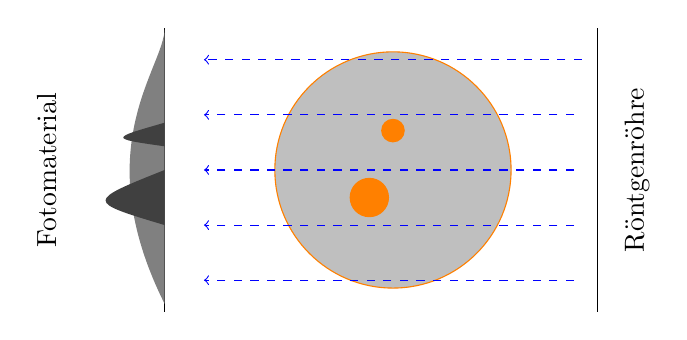
\begin{tikzpicture}[domain=3:3]  
	
	\fill[lightgray] (0.9,0.7) circle (1.5cm);
	
	\draw [rotate=90, yshift=2cm, -](-1.1,0) -- (2.5,0); % s-Achse
	
	\draw  (-0.5, 0.7) node [rotate=90, yshift=3cm] {Fotomaterial};
	
	\fill[gray] [rotate=90, yshift=2cm] (-1,0) .. controls (1,1) and (2,0) .. (2.5,0);
	\fill[darkgray] [rotate=90, yshift=2cm] (0,0) .. controls (0.3,1)  .. (0.7,0);
	\fill[darkgray] [rotate=90, yshift=2cm] (1,0) .. controls (1.1,0.7)  .. (1.3,0);
	
	\draw[orange] (0.9,0.7) circle (1.5cm);
	\fill[orange] (0.9,  1.2) circle (.15cm);
	\fill[orange] (0.6, 0.35) circle (.25cm);
	
	\draw [rotate=90, dashed, ->] [blue] (0,-3.2) -- (0,1.5); % strahl
	\draw [rotate=90, xshift=-0.7cm, dashed, ->] [blue] (0,-3.2) -- (0,1.5); % strahl
	\draw [rotate=90, xshift=0.7cm, dashed, ->] [blue] (0,-3.2) -- (0,1.5); % strahl
	\draw [rotate=90, xshift=1.4cm, dashed, ->] [blue] (0,-3.2) -- (0,1.5); % strahl
	\draw [rotate=90, xshift=2.1cm, dashed, ->] [blue] (0,-3.3) -- (0,1.5); % strahl
	
	\draw [rotate=90, yshift=-3.5cm, -](-1.1,0) -- (2.5,0); % Sensor-Achse
	\draw  (3, 0.7) node [rotate=90, yshift=-1cm, -] {Röntgenröhre};
	
	\begin{scope}[xshift=1cm]
	\end{scope}
	
	\end{tikzpicture}
	\caption{Schematischer Aufbau einer Röntgenaufnahme im Draufsicht. Links ist das Schwächungsprofil nach Durchgang der Röntgenstrahlen durch ein Medium mit verschiedenen Dichten zu sehen (mit der Annahme, dass orangene Kreise höhere Dichte haben, als die graue Fläche).}
	\label{fig:1.1}
\end{figure}
%----------------------------------------------------------------------------------------
%	Ende der Grafik
%----------------------------------------------------------------------------------------

Sicherlich wäre die Computertomographie ohne die Röntgenstrahlung nicht denkbar. Diese verdankt ihren Namen dem deutschen Physiker Wilhelm Conrad Röntgen (1845-1923). Im Jahre 1895 gelang es ihm zum ersten Mal eine elektromagnetische Strahlung zu erzeugen, deren Wellenlänge zwischen 10$nm$ und 1$pm$ lag. Solche kurze Wellenlängen haben nur energiereiche Strahlen. Das erlaubt ihnen die Durchdringung der Materie. Anzumerken ist, dass die Intensität hochenergetischer Strahlen beim Durchgehen der Materie mit der Eindringtiefe abfällt. Dies bedeutet, dass die Röntgenstrahlung beim Auftreffen auf ein Probestück eine höhere Intensität besitzt als beim Austreten. Bei den herkömmlichen Röntgenaufnahmen wurde diese Eigenschaft direkt ausgenutzt und man hat überlagerte Schatten von Objekten mit verschiedenen Dichten auf das Aufnahmematerial projiziert bekommen. Damit erschienen die dichteren Stellen des Objekts dunkler, weiche entsprechend heller. Für gewisse Situationen geben solche Projektionen genug Information her, jedoch nicht, wenn die räumliche Anordnung des Inneren eines Objekts diskutiert werden soll (Abb.\ref{fig:1.1}).

Um das Problem der räumlichen Anordnung der Objekte zu lösen, ist folgendes Vorgehen sehr nützlich. Würde man das Schattenbild aus der Abbildung \ref{fig:1.1} zurück in die Schnittebene des Objekts projizieren, so wie es in der Abbildung \ref{fig:1.2} (a) gezeigt ist, erhält man etwas Information über die gegebene Objekte. Projiziert man mehrere Schattenbilder, die aus verschiedenen Winkeln aufgenommen worden sind, so erhält man als Summe der Rückprojektionen, die sogenannte Rückprojektion(Abb. \ref{fig:1.2}(b)). Später werden wir sehen, welcher mathematischer Aufwand sich hinter dieser Idee verbirgt, bevor ein annehmbares Resultat zustande kommt.

%----------------------------------------------------------------------------------------
%	Beginn der Grafik
%----------------------------------------------------------------------------------------
\begin{figure}[!h]
	\centering\small
	\begin{tabular}{cc}
		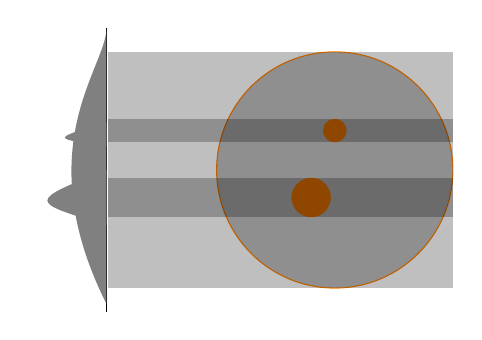
\begin{tikzpicture}[domain=3:3]  
		
		\fill[lightgray] (0.9,0.7) circle (1.5cm);
		
		\draw [rotate=90, yshift=2cm, - ](-1.1,0) -- (2.5,0); % s-Achse
		
		\fill[gray] [rotate=90, yshift=2cm] (-1,0) .. controls (1,1) and (2,0) .. (2.5,0);
		\fill[gray] [rotate=90, yshift=2cm] (0,0) .. controls (0.3,1)  .. (0.7,0);
		\fill[gray] [rotate=90, yshift=2cm] (1,0) .. controls (1.1,0.7)  .. (1.3,0);
		
		\draw[orange] (0.9,0.7) circle (1.5cm);
		\fill[orange] (0.9,  1.2) circle (.15cm);
		\fill[orange] (0.6, 0.35) circle (.25cm);
		
		\fill[nearly transparent] (-1.98,-0.8) rectangle (2.4,2.2);
		
		\fill[nearly transparent] (-1.98,0.1) rectangle (2.4,0.6);
		\fill[nearly transparent] (-1.98,1.05) rectangle (2.4,1.35);
		\begin{scope}[xshift=1cm]
		\end{scope}
		
		\end{tikzpicture} &	
		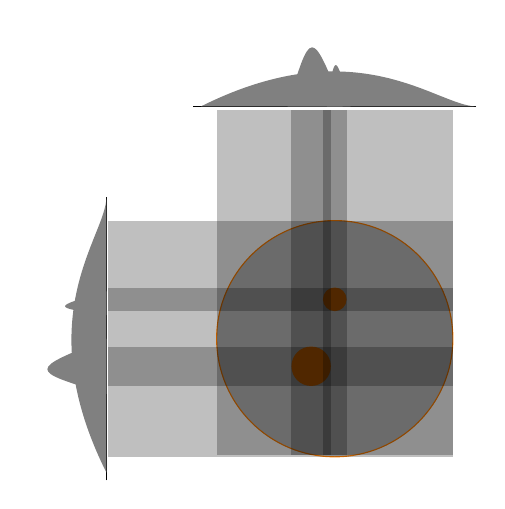
\begin{tikzpicture}[domain=3:3]  
		
		\fill[lightgray] (0.9,0.7) circle (1.5cm);
		
		\draw [rotate=90, yshift=2cm](-1.1,0) -- (2.5,0); % s-Achse
		
		\fill[gray] [rotate=90, yshift=2cm] (-1,0) .. controls (1,1) and (2,0) .. (2.5,0);
		\fill[gray] [rotate=90, yshift=2cm] (0,0) .. controls (0.3,1)  .. (0.7,0);
		\fill[gray] [rotate=90, yshift=2cm] (1,0) .. controls (1.1,0.7)  .. (1.3,0);
		
		\draw[orange] (0.9,0.7) circle (1.5cm);
		\fill[orange] (0.9,  1.2) circle (.15cm);
		\fill[orange] (0.6, 0.35) circle (.25cm);
		
		\fill[nearly transparent] (-1.98,-0.8) rectangle (2.4,2.2);
		
		\fill[nearly transparent] (-1.98,0.1) rectangle (2.4,0.6);
		\fill[nearly transparent] (-1.98,1.05) rectangle (2.4,1.35);
		\begin{scope}[xshift=1cm]
		\end{scope}
		
		\draw [rotate=0, yshift=3.65cm, xshift=0.2cm](-1.1,0) -- (2.5,0); % s-Achse
		
		\fill[gray] [rotate=0, yshift=3.65cm, xshift=0.2cm] (-1,0) .. controls (1,1) and (2,0) .. (2.5,0);
		\fill[gray] [rotate=0, yshift=3.65cm, xshift=0.3cm] (0,0) .. controls (0.3,1)  .. (0.7,0);
		\fill[gray] [rotate=0, yshift=3.65cm, xshift=-0.2cm] (1,0) .. controls (1.1,0.7)  .. (1.3,0);
		
		\fill[ nearly transparent] [rotate=90, xshift=1.1cm, yshift=-1.6cm] (-1.88,-0.8) rectangle (2.5,2.2);
		
		\fill[nearly transparent] [rotate=90, xshift=1.1cm, yshift=-0.95cm] (-1.88,0.1) rectangle (2.5,0.6);
		\fill[nearly transparent] [rotate=90, xshift=1.1cm, yshift=-2.1cm] (-1.88,1.05) rectangle (2.5,1.35);
		
		\end{tikzpicture}\\	
		(a) & (b) 
	\end{tabular}
	\caption{Das Prinzip der Bildrekonstruktion aus CT-Daten mit einer Rückprojektion~(a) und zwei Rückprojektionen~(b).} 
	\label{fig:1.2}
\end{figure}
%----------------------------------------------------------------------------------------
%	Ende der Grafik
%----------------------------------------------------------------------------------------

Ein Pionier der Tomographie, A. M. Cormack\footnote{\label{foot:1} Allan M. Cormack (1924-1998) südafrikanischer Physiker.}, veröffentlichte 1964 eine Arbeit über die mathematische Bestimmung der Dichten eines Objekts. Aus den Projektionsdaten konnte er die innere Dichteverteilung des Objekts bestimmen.

Der erste Prototyp eines CT-Scanners wurde vom G. N. Hounsfield\footnote{\label{foot:2} Godfrey N. Hounsfield (1919 - 2004) englischer Ingenieur.} im Jahr 1968 entwickelt. Seine Arbeit beruhte auf den Erkenntnissen von M. Cormack. Die Idee, der um das Objekt rotierenden Scanneinheit (Abb. \ref{fig:1.3}) findet man hier wieder. Vorerst konnten nur anatomische Präparate vermessen werden. Aber schon im Jahre 1972 entstehen erste klinische Untersuchungen mit einem Schädelscanner durch Hounsfield und Ambrose. 1973 werden Berichte über die Weichteildiagnostik des Gehirns mithilfe eines CT-Scanners veröffentlicht. Hinsichtlich der Nützlichkeit des CT-Verfahrens in der Medizin, wurden A. M. Cormack und G. N. Hounsfield im Jahre 1979 mit dem Nobelpreis für Medizin ausgezeichnet. 

In darauf folgenden Jahren entstand eine ganze Reihe von Generationen des CT-Scanners. Die Hauptunterschiede bestehen in der Komposition der Scanneinheit und dessen Technik, siehe auch \cite[Kap.\ 3]{Buzug04}. Heutzutage hat sich die dritte Genration am meisten durchgesetzt. Der prinzipielle Grundaufbau (Abb. \ref{fig:1.3}) dieses Scanners besteht darin, dass die Röntgenröhre und Detektor fest auf einem Ringkörper, einander gegenüber installiert sind. In der Mitte des Rings ist ein fest installierter Probetisch, sodass die Scanneinheit um diesen rotieren kann. Mittels dieser Konstruktion ist es möglich \textit{tomographische} Bilddaten aus allen Positionen um die Längsachse des Objekts aufzunehmen.
%----------------------------------------------------------------------------------------
%	Beginn der Grafik
%----------------------------------------------------------------------------------------
\begin{figure}[!h]
	
	\centering
	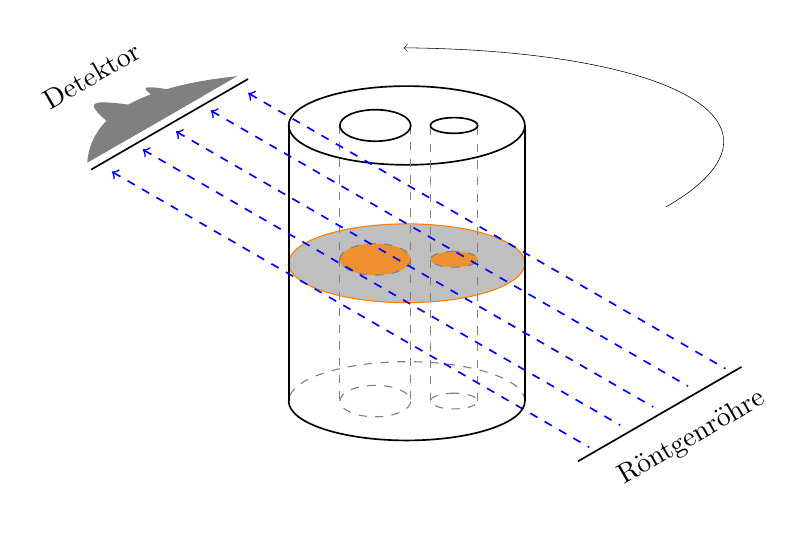
\begin{tikzpicture}
	%\draw[dashed,color=gray] [rotate=90, xshift=0cm, yshift=1.5cm] (-1,0) -- (4.4,0);% right line
	
	\draw[dashed,color=gray][rotate=90] (0,0) arc (-90:90:0.5 and 1.5);% top half of the bottom ellipse
	
	\draw[semithick][rotate=90] (4,1.5) arc (0:360:0.5 and 1.5);
	\draw[very thin, ->][rotate=95] (2.3,-2) arc (240:340:1.6 and 6);
	
	\fill[nearly transparent][rotate=90] (2.25,1.5) arc (0:360:0.5 and 1.5); % middle ellipse
	
	% inner lines
	\draw[dashed,color=gray] [rotate=90] (0,1.2) -- (3.5,1.2);% left line of inner small ellipse 
	\draw[dashed,color=gray] [rotate=90] (0,0.6) -- (3.5,0.6);% right line of the inner small ellipse
	
	\draw[dashed,color=gray] [rotate=90] (3.5, 2.35) -- (0, 2.35);% right line of the inner big ellipse
	\draw[dashed,color=gray] [rotate=90] (3.5, 1.45) -- (0, 1.45);% left line of the inner big ellipse
	
	% inner top ellipses
	\draw[semithick] [rotate=90] (3.5, .9) ellipse (0.1 and .3); % top small inner ellipse
	\draw[semithick] [rotate=90] (3.5, 1.9) ellipse (0.2 and .45); % top big inner ellipse
	
	% inner middle ellipses
	\fill[nearly opaque,color=orange] [rotate=90] (1.8, .9) ellipse (0.1 and .3);% middle small inner ellipse
	\fill[nearly opaque,color=orange] [rotate=90] (1.8, 1.9) ellipse (0.2 and .45); % middel big inner ellipse
	\draw[dashed,color=gray] [rotate=90] (1.8, .9) ellipse (0.1 and .3);% middle small inner ellipse
	\draw[dashed,color=gray] [rotate=90] (1.8, 1.9) ellipse (0.2 and .45); % middel big inner ellipse
	
	
	% inner bottom ellipses
	\draw[dashed,color=gray] [rotate=90] (0, .9) ellipse (0.1 and .3); % bottom small inner ellipse
	\draw[dashed,color=gray] [rotate=90] (0, 1.9) ellipse (0.2 and .45); % bottom big innerellipse
	
	\draw[color=orange][rotate=90] (2.25,1.5) arc (0:360:0.5 and 1.5); % middle ellipse
	
	%sids lines
	\draw[semithick] [rotate=90] (0,0) -- (3.5,0);% right line
	\draw[semithick] [rotate=90] (0,3) -- (3.5,3);% left line
	
	% Röntgenröhre
	\draw [semithick] [rotate=30, xshift=0.cm, yshift=-1.0cm](0.2,0) -- (2.6,0); % Röntgenröhre
	\draw  (1.5,-1.4) node [rotate=30, xshift=1.cm, yshift=0.5cm] { Röntgenröhre};
	
	\draw [semithick] [rotate=30, xshift=-3.5cm, yshift=5.3cm](0.2,0) -- (2.5,0); % Detektorachse
	\draw  (1.5,-1.4) node [rotate=30, xshift=-3.3cm, yshift=8.3cm] {Detektor};
	
	\draw [dashed, semithick, <-, blue] [rotate=150, , xshift=1.cm, yshift=0.1cm](5,0) -- (-2,0);
	\draw [dashed, semithick, <-, blue] [rotate=150, , xshift=0.8cm, yshift=-0.34cm](5,0) -- (-2,0);
	\draw [dashed, semithick, <-, blue] [rotate=150, , xshift=0.55cm, yshift=-0.75cm](5,0) -- (-2,0);
	\draw [dashed, semithick, <-, blue] [rotate=150, , xshift=0.3cm, yshift=-1.2cm](5,0) -- (-2,0);
	\draw [dashed, semithick, <-, blue] [rotate=150, , xshift=3.cm, yshift=-1.63cm](2,0) -- (-5,0);
	
	\fill[gray] [rotate=30, yshift=5.4cm, xshift=-3cm] (-0.3,0) .. controls (0.1,0.6) and (1,0.4) .. (1.9,0);
	\fill[gray] [rotate=30, yshift=5.4cm, xshift=-3cm] (0.3,0) .. controls (0,0.8)  .. (1,0);
	\fill[gray] [rotate=30, yshift=5.4cm, xshift=-3cm] (1,0) .. controls (0.7,0.6)  .. (1.4,0);
	
	\draw[semithick] [rotate=90] (0,0) arc (270:90:0.5 and 1.5);% bottom half of the bottom ellipse
	
	\end{tikzpicture}
	\caption{Prinzipieller Aufbau eines CT-Scanners der dritten Generation.}
	\label{fig:1.3}
\end{figure}
%----------------------------------------------------------------------------------------
%	Ende der Grafik
%----------------------------------------------------------------------------------------
Die oben beschriebene Rückprojektion aller tomographischen Daten (Projektionen) erzeugt ein Schnittbild. Erzeugt man mehrere Schnittbilder entlang der Längsachse des Objekts, so kann man diese der Reihe nach aufstellen und mithilfe programmiertechnischer Werkzeuge ein dreidimensionales Bild dieses Objekts gewinnen (Abb. \ref{fig:1.4}) .
%----------------------------------------------------------------------------------------
%	Beginn der Grafik
%----------------------------------------------------------------------------------------
\begin{figure}[h]
	\centering
	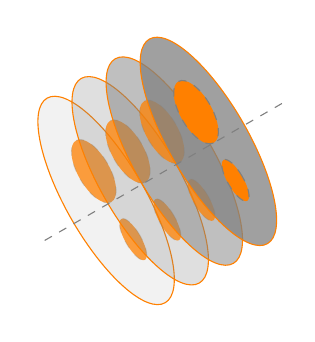
\begin{tikzpicture}
	
	\fill[very nearly transparent, color=gray][rotate=30] (2.25,1.5) arc (0:360:0.5 and 1.5); % middle ellipse
	
	% inner middle ellipses
	\fill[nearly opaque,color=orange] [rotate=30] (1.8, .9) ellipse (0.1 and .3);% middle small inner ellipse
	\fill[nearly opaque,color=orange] [rotate=30] (1.8, 1.9) ellipse (0.2 and .45); % middel big inner ellipse
	\draw[nearly transparent, dashed,color=gray] [rotate=30] (1.8, .9) ellipse (0.1 and .3);% middle small inner ellipse
	\draw[nearly transparent, dashed,color=gray] [rotate=30] (1.8, 1.9) ellipse (0.2 and .45); % middel big inner ellipse
	
	\draw[color=orange][rotate=30] (2.25,1.5) arc (0:360:0.5 and 1.5); % middle ellipse
	
	%--------- second slice
	
	\fill[nearly transparent, color=gray][rotate=30, xshift=0.5cm] (2.25,1.5) arc (0:360:0.5 and 1.5); % middle ellipse
	
	% inner middle ellipses
	\fill[nearly opaque,color=orange] [rotate=30, xshift=0.5cm] (1.8, .9) ellipse (0.1 and .3);% middle small inner ellipse
	\fill[nearly opaque,color=orange] [rotate=30, xshift=0.5cm] (1.8, 1.9) ellipse (0.2 and .45); % middel big inner ellipse
	\draw[nearly transparent, dashed,color=gray] [rotate=30, xshift=0.5cm] (1.8, .9) ellipse (0.1 and .3);% middle small inner ellipse
	\draw[nearly transparent, dashed,color=gray] [rotate=30, xshift=0.5cm] (1.8, 1.9) ellipse (0.2 and .45); % middel big inner ellipse
	
	\draw[color=orange][rotate=30, xshift=0.5cm] (2.25,1.5) arc (0:360:0.5 and 1.5); % middle ellipse
	
	%--------- third slice
	
	\fill[semitransparent, color=gray][rotate=30, xshift=1cm] (2.25,1.5) arc (0:360:0.5 and 1.5); % middle ellipse
	
	% inner middle ellipses
	\fill[nearly opaque, color=orange] [rotate=30, xshift=1cm] (1.8, .9) ellipse (0.1 and .3);% middle small inner ellipse
	\fill[nearly opaque, color=orange] [rotate=30, xshift=1cm] (1.8, 1.9) ellipse (0.2 and .45); % middel big inner ellipse
	\draw[nearly transparent, dashed,color=gray] [rotate=30, xshift=1cm] (1.8, .9) ellipse (0.1 and .3);% middle small inner ellipse
	\draw[nearly transparent, dashed,color=gray] [rotate=30, xshift=1cm] (1.8, 1.9) ellipse (0.2 and .45); % middel big inner ellipse
	
	\draw[color=orange][rotate=30, xshift=1cm] (2.25,1.5) arc (0:360:0.5 and 1.5); % middle ellipse
	
	%--------- fourd slice	
	
	\fill[nearly opaque, color=gray] [rotate=30, xshift=1.5cm] (2.25,1.5) arc (0:360:0.5 and 1.5); % middle ellipse
	
	% inner middle ellipses
	\fill[color=orange] [rotate=30, xshift=1.5cm] (1.8, .9) ellipse (0.1 and .3);% middle small inner ellipse
	\fill[color=orange] [rotate=30, xshift=1.5cm] (1.8, 1.9) ellipse (0.2 and .45); % middel big inner ellipse
	\draw[dashed,color=gray] [rotate=30, xshift=1.5cm] (1.8, .9) ellipse (0.1 and .3);% middle small inner ellipse
	\draw[dashed,color=gray] [rotate=30, xshift=1.5cm] (1.8, 1.9) ellipse (0.2 and .45); % middel big inner ellipse
	
	\draw[color=orange] [rotate=30, xshift=1.5cm] (2.25,1.5) arc (0:360:0.5 and 1.5); % middle ellipse
	
	\draw[dashed,color=gray] [rotate=30, xshift=0.8cm] (3.5, 1.45) -- (0, 1.45); % axisis
	
	\end{tikzpicture}
	\caption{Das Schichtmodell eines Objekts als Grundlage zur dreidimensionalen Rekonstruktion.}
	\label{fig:1.4}
\end{figure} 
%----------------------------------------------------------------------------------------
%	Ende der Grafik
%----------------------------------------------------------------------------------------

Im Folgenden gehen wir mehr auf die mathematisch-physikalischen Gegebenheiten der oben beschriebenen Situation ein. 

\section{Die Radon Transformation}
\label{cha:1.2}

Das Verständnis des mathematischen Problems der Bildrekonstruktion in der Computertomographie verlangt zunächst das Verständnis der Entstehung der tomographischen Bilddaten. Die Entstehung solcher Daten kann mithilfe eines mathematischen Modells nachvollzogen werden. Bekanntlich baut man das mathematische Modell auf physikalischen Annahmen auf. Die Abbildung \ref{fig:1.5} soll in diesem Fall als physikalisches Ausgangsmodell dienen. Wir nehmen an, dass der graue Kreis eine homogene Dichteverteilung besitzt. Unter weiteren Annahme sollen die Röntgenstrahlen sich geradlinig ohne Streuung in Richtung des Detektors ausbreiten.

Sei nun $f(x,y)$ die gesuchte Dichtefunktion, die auf einem Einheitskreis $\Omega = \{ (x,y) \in \R^2 \ | \ x^2 + y^2 \leq 1 \}$ definiert ist. Dass $f$ auf einem Kreis liegen soll, folgern wir aus der physikalischen Situation. Das Objekt wird aus einem bestimmten Radius um den Mittelpunkt der Scanneinheit gescannt, daher möchten wir, dass ein Objekt in die CT-Scanneinheit passt, gegebenenfalls muss die Scanneinheit skaliert werden.

Die blau gestrichelte Linie in Abbildung \ref{fig:1.5} stelle einen Röntgenstrahl dar. Wir möchten das Verhalten der Intensität entlang der Strahllinie an den Punkten $L_0$ und $L_0 + \Delta L$ beobachten. Wie schon erwähnt wurde, nimmt die Intensität $I$ der Röntgenstrahlen mit der Eindringtiefe in das Objekt ab. Das Verhalten ist in der Physik unter dem Namen \textit{Lambert-Beer’sches Gesetz} bekannt und besagt:
\begin{center}
	\textit{Die Intensitätsabnahme der Strahlung ist proportional zur Intensität. Der Proportionalitätsfaktor hängt von der Art der durchdrungenen Materie ab.}
\end{center}
\begin{equation}
	I(L_0 + \Delta L) - I(L_0) = - \alpha I(L_0).
	\label{equa:1.1}
\end{equation}
Der Proportionalitätsfaktor $\alpha$ ist durch das Produkt der Dichteverteilung entlang des Strahls, also $f(L)$ und seiner zurückgelegten Strecke $\parallel \Delta L\parallel$ gegeben. Hier wird angenommen, dass $f(L)$ die Eigenschaften des Materials in sich trägt. Insgesamt ergibt sich
\begin{equation}
	I(L_0 + \Delta L) - I(L_0) = -f(L) \parallel \Delta L \parallel I(L_0).
	\label{equa:1.2}
\end{equation}
Nimmt man an, dass die Gleichung (\ref{equa:1.2}) asymptotisch im Sinne $\parallel \Delta L \parallel \rightarrow 0$ verstanden werden kann, so kann die linke Seite von (\ref{equa:1.2}) als Ableitung von $I$ nach $L$ interpretiert werden und man schreibt:
\begin{equation}
	\lim_{\Delta L\rightarrow 0}\frac{I(L_0 + \Delta L) - I(L_0)}{\parallel \Delta L \parallel} = \frac{\partial I}{\partial L} = -f(L)I(L_0).
	\label{equa:1.3}
\end{equation}
Mit \ref{equa:1.3} liegt eine lineare Differentialgleichung (DGL) erster Ordnung vor. Diese DGL kann mithilfe einfacher analytischer Werkzeuge, wie Variablenseparation gelöst werden. 
%----------------------------------------------------------------------------------------
%	Beginn der Grafik
%----------------------------------------------------------------------------------------
\begin{figure}[!h]
	\centering
	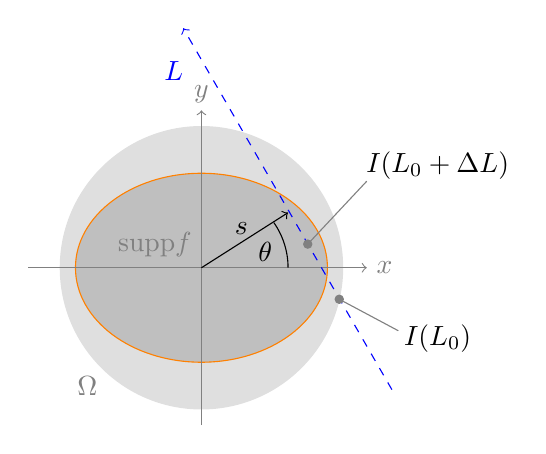
\begin{tikzpicture}

	\fill[nearly transparent, color=gray] (0.9,0) circle (1.8cm);
	
	\fill[lightgray] (0.9,0) ellipse (1.6cm and 1.2cm);	
	
	\draw[orange] (0.9,0) ellipse (1.6cm and 1.2cm);
	
	\draw [gray] [->](-1.3,0) -- (3,0); % x-Achse
	\draw [gray] (3, 0) node [right] {$x$};
	
	\draw [gray] [->](0.9,-2) -- (0.9,2); % y-Achse
	\draw [gray] (0.9, 2.2) node {$y$};
	
	\draw[gray](0.9, 0.3) node [left] {$\mbox{supp}f$};
	
	\draw[->] (0.9,0) -- (2, 0.7);
	\draw(1.2, 0.5)  node [right] {$s$};
	
	\draw [rotate=30, xshift=2.1cm, dashed, ->] [blue] (0,-3) -- (0,2.3); % strahl
	\draw [blue] (0.55, 2.5)  node {$L$};
	
	\draw(2,0) arc [start angle=0, end angle=35, radius=1cm];
	\draw(1.5, 0.2) node [right] {$\theta$};
	
	\draw [gray] (-0.8, -1.5) node [right] {$\Omega$};
	
	\draw(3.9, 1.3) node {$I(L_0 + \Delta L)$};
	\fill[gray](2.25, 0.3) circle [radius=0.06];
	\draw[-,thin,gray](2.25, 0.3) -- (3, 1.1);
	
	\draw(3.9, -0.9) node {$I(L_0)$};
	\fill[gray](2.65, -0.4) circle [radius=0.06];
	\draw[-,thin,gray](2.65, -0.4) -- (3.4, -0.8);
	
	\end{tikzpicture}	
	\caption{Intensitätsänderung der Röntgenstrahlung beim Passieren eines homogenen Objekts.}
	\label{fig:1.5}
\end{figure}
%----------------------------------------------------------------------------------------
%	Ende der Grafik
%----------------------------------------------------------------------------------------
Nach der Separation der Variablen in (\ref{equa:1.3}) und anschließender Integration bekommt man nun folgenden Ausdruck
\begin{equation}
	\ln(\frac{I_1}{I_0}) = -\int_{L_0}^{L_1} f(L) \mbox{d} L.
	\label{equa:1.4}
\end{equation}
Durch das Exponentieren von (\ref{equa:1.4}) gelangt man zu dem \textit{Lambert-Beer’schen Gesetz} $I(L_1) = I_0 e^{-\int_{L_0}^{L_1} f(L) \mbox{d} L}$. Jedoch für die Zwecke der Computertomographie interessiert man sich für etwas von (\ref{equa:1.4}) abgewandelte Darstellung
\begin{equation}
	\ln(\frac{I_0}{I_1}) = \int_{L_0}^{L_1} f(L) \mbox{d} L.
	\label{equa:1.5}
\end{equation} 
Die rechte Seite in (\ref{equa:1.5}) liefert einen Summenwert von $f$ entlang der Geraden $L$ (Abb. \ref{fig:1.6}), die wie folgt parametrisiert werden kann:
\begin{equation}
	\begin{matrix}
		L(s, \theta, t) & = & s\begin{pmatrix} \cos(\theta) \\ \sin(\theta) \end{pmatrix} & + & t\begin{pmatrix} -\sin(\theta) \\ \cos(\theta)  \end{pmatrix} \\ \\
		& = & s\omega(\theta) & + & t\omega^{\perp}(\theta)
	\end{matrix} \ , \ \ s, t \in \R; \ \theta \in [0,\pi].
	\label{equa:1.6}
\end{equation}
Betrachtet man alle Geraden, die den Einheitskreis schneiden, dann ergibt sich folgende Menge
\begin{equation}
	G = \{ L(s, \theta, t) \ | \ |s| \leq 1, \  \theta \in [0,\pi] \ t \in [-\gamma(s), \gamma(s)] \}.
	\label{equa:1.7}
\end{equation}
Wobei $\gamma(s)$ den Parameter $t$ für (\ref{equa:1.6}) festlegt und folgendermaßen definiert werden kann
\begin{equation}
	\gamma(s) = \left\{ \begin{matrix}
	\sqrt{1 - s^2} & : & |s| \leq 1 \\ 
	0 & : & \mbox{sonst}
	\end{matrix}.
	\right.
	\label{equa:1.8}
\end{equation}
Die Gleichung (\ref{equa:1.8}) liefert nun die Integrationsgrenzen für (\ref{equa:1.5}). Da die Werte von $\pm\gamma(s)$ genau die Schnittpunkte von $L$ mit $\Omega$ liefern und  $\mbox{supp} f$\footnote{\label{foot:3} Mit $\mbox{supp} f$ (Support) ist der Träger einer Funktion $f$ gemeint. Def.: $\mbox{supp} f := \overline{ \{ x \in \Omega | f(x) \neq 0 \} } $} $\subseteq \Omega$, heißt es insgesamt, dass nur die Werte von $L \subset \mbox{supp} f$ bei der Integration von (\ref{equa:1.5}) berücksichtigt werden.

Kehren wir zur Gleichung (\ref{equa:1.5}) zurück und betrachten die Abbildung \ref{fig:1.6}, werden wir feststellen, dass die Funktion $f$ über den Parameter $t$ integriert werden muss. Hierzu bedarf es einer Variablentransformation:
\begin{equation}
	\begin{matrix}
		|(J(L))| = \left|\begin{pmatrix} \cos(\theta) & \sin(\theta)\\ -\sin(\theta) & \cos(\theta) \end{pmatrix}\right| = 1 \\ \\
		\mbox{und} \\ \\
		\mbox{d}L = \mbox{det}(J(L)) \mbox{d}t .
	\end{matrix}
	\label{equa:1.9}
\end{equation}
%----------------------------------------------------------------------------------------
%	Beginn der Grafik
%----------------------------------------------------------------------------------------
\begin{figure}[!h]
	\centering
	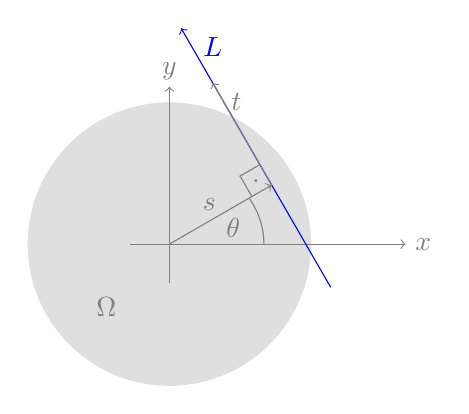
\begin{tikzpicture}
	
	\fill[nearly transparent, color=gray] (0,0) circle (1.8cm);
	
	\draw [gray] [->](-0.5,0) -- (3,0); % x-Achse
	\draw [gray] (3, 0) node [right] {$x$};
	
	\draw [gray] [->](0,-0.5) -- (0,2); % y-Achse
	\draw [gray] (0, 2.2) node {$y$};
	
	\draw [rotate=30, xshift=1.5cm, ->] [blue] (0,-1.5) -- (0,2.3); % strahl	
	\draw [blue] (0.55, 2.5)  node {$L$};%{$\omega^{\perp}$};
	
	\draw [rotate=30, xshift=1.5cm, ->] [gray ] (0,0) -- (0,1.5);
	\draw [gray] (0.85,1.8) node {$t$}; 
	
	\draw [xshift=1.05cm, yshift=0.6cm, rotate=120, - ] [gray] (0,0) -- (0.3,0);
	\draw [xshift=0.89cm, yshift=0.86cm, rotate=30, - ] [gray] (0,0) -- (0.3,0);
	\draw [gray] (1.1, 0.8)  node {$.$};
	
	\draw [rotate=30] [gray] [->] (0,0) -- (1.5, 0);
	\draw [gray] (0.3, 0.5)  node [right] {$s$};
	
	\draw [gray] (1.2,0) arc [start angle=0, end angle=35, radius=1cm];
	\draw [gray] (0.6, 0.2) node [right] {$\theta$};
	
	\draw [gray] (-0.8, -0.8) node {$\Omega$};
	
	\end{tikzpicture}
	\caption{Parametrisierung des Strahls $L$ auf dem Gebiet $\Omega$. }
	\label{fig:1.6}
\end{figure}
%----------------------------------------------------------------------------------------
%	Ende der Grafik
%----------------------------------------------------------------------------------------

Mit den obigen Abmachungen haben wir nun alles Nötige in der Hand, um die Radon\footnote{\label{foot:4} Johann Karl August Radon (1887-1956) österreichischer Mathematiker.} Transformation angeben zu können. 
\begin{Definition}
	Sei nun $f:\Omega \subseteq \R^2 \rightarrow \R$ eine integrierbare Funktion, dann ist ihre Radon Transformation durch
	\begin{equation}
		\mathcal{R}f(s,\theta) := \int\limits_{-\gamma(s)}^{\gamma(s)} f(s\omega(\theta) + t\omega^{\perp}(\theta)) \mbox{d}t
		\label{equa:1.10}
	\end{equation}
	definiert. Hier ist $\Omega = \{ (x,y) \in \R^2 \ | \ x^2 + y^2 \leq 1 \}$.
	\label{def.1}
\end{Definition}

\begin{Bemerkung}
	$\mathcal{R}$ wird als Integraloperator oder einfach als Operator bezeichnet.
	\label{bem:1} 
\end{Bemerkung}

Die Gleichung (\ref{equa:1.10}) trägt das Wesen der Computertomographie in sich und gehört in den Bereich der Integraltransformationen. In der Tat ist man aber an der Inversion von $\mathcal{R}$ interessiert. Das wird klarer, wenn man (\ref{equa:1.10}) etwas anders auffasst:
\begin{equation}
	p(s,\theta) = \mathcal{R}f(s,\theta).
	\label{equa:1.11}
\end{equation}
Somit stellt $p(s,\theta)$ in (\ref{equa:1.11}) genau die Projektion einer unbekannten Dichteverteilung entlang eines Röntgenstrahls $L(s,\theta)$ dar. Da die Projektionen als Messwerte beim CT-Verfahren entstehen, möchte man $f$ folgendermaßen wiedergewinnen 
\begin{equation}
	f(x) = \mathcal{R}^{-1}p(x).
	\label{equa:1.12}
\end{equation}
Jedoch offenbaren sich einige mathematische Hürden bei der Inversion von (\ref{equa:1.10}), was die Rekonstruktion von $f$ aus den Projektionsdaten schwierig macht. Um die dahinterstehende Problematik besser verstehen zu können, untersuchen wir zunächst die Eigenschaften von (\ref{equa:1.10}).

\subsection{Kleiner Einschub über $L^2$-Raum}
\label{cha:1.2.1}

Um den Operator $\mathcal{R}$ untersuchen zu können, sollte man wissen auf welchen Räumen er operiert. Dieses Wissen erlaubt uns Aussagen über die Stetigkeit, Kompaktheit und auch über die Singulärwertzerlegung (SWZ) von $\mathcal{R}$ zu treffen. Besonders wichtig ist die SWZ, denn anhand dieser ergibt sich eine Möglichkeit den Operator $\mathcal{R}$ zu invertieren. Zudem wollen wir im nächsten Kapitel die Schlechtgestelltheit des computertomographischen Problems diskutieren, welche die Eigenschaften der SWZ benutzt.

In Bezug auf das hier vorgestellte Rekonstruktionsproblem der Computertomographie betrachten wir Funktionen auf dem Gebiet $\Omega \subset \R^2$. Wir setzen voraus, dass die Funktionen auf $\Omega$ integrierbar sind. Wie dieser Sachverhalt zu verstehen ist, wollen wir kurz und grob andeuten.

Zunächst klären wir den Begriff der Integrierbarkeit einer Funktion im Sinne von Lebesgue\footnote{Henri Léon Lebesgue (1875-1941) französischer Mathematiker.}. Das Lebesgue-Integral wird für Funktionen auf einem geeigneten Maßraum definiert. Ein Maßraum ist durch ein Tripel $( \Omega, \mathcal{A}, \lambda)$ gegeben.

Eine sogenannte $\sigma$-\textit{Algebra} $\mathcal{A} \subset \mathcal{P}(\Omega)$ auf $\Omega$ ist ein Mengensystem bestehend aus Teilmengen von $\Omega$. $\mathcal{A}$ besitzt folgende Eigenschaften: (\lowroman{1}). Jede endliche oder abzählbar unendliche Vereinigung oder jeder Durchschnitt der Elemente aus $\mathcal{A}$ liegen wieder in $\mathcal{A}$, sowie $\Omega$ und $\emptyset$. (\lowroman{2}). Die Komplemente der Elemente aus $\mathcal{A}$, also $\forall A \in \mathcal{A} : \Omega \setminus A = A^\mathrm{C} \in \mathcal{A}$ , liegen auch in $\mathcal{A}$.

Nun suchen wir eine Funktion, die allen Elementen $A$ aus $\mathcal{A}$ eine positive Zahl zuordnet, also $\lambda(A) \in [0, \infty]$. Somit beschreibt $\lambda$ das Maß einer Menge in $\mathcal{A}$. Im Falle $\Omega \subset \R^2$ ordnet $\lambda$ den Flächeninhalt einer Teilmenge von $\Omega$ zu. Des Weiteren hat $\lambda$ folgende Eigenschaften: (\lowroman{1}): $\lambda(\emptyset) = 0$ und (\lowroman{2}): die $\sigma$-\textit{Additivität}, das heißt für paarweise disjunkte Mengen $(A_n)_{n \in \N}$ aus $\mathcal{A}$ gilt
 
\[ \lambda \left(  \bigcup\limits_{n=1}^{\infty} A_n \right) = \sum\limits_{n = 1}^{\infty} \lambda(A_n).\]  

Nun gilt per Definition \textit{messbarer Abbildungen} zwischen zwei Maßräumen, dass die Urbilder messbarer Mengen messbar sind. Das heißt $f:(X_1, \mathcal{A}_1) \rightarrow (X_2, \mathcal{A}_2)$ ist messbar, wenn für alle $A_{2_j} \in \mathcal{A}_2$ gilt $f^{-1}(A_{2_j}) \in \mathcal{A}_1$. 

Um den Begriff der Integrierbarkeit im Sinne von Lebesgue einführen zu können, fehlt uns noch der Begriff der Borel\footnote{Émile Borel (1871-1956)  französischer Mathematiker.}-$\sigma$-Algebra. Dazu benutzen wir für uns relevante mengen $\R$ und $\R^2$. Das ist insofern klar, weil die gesuchten Dichtefunktionen in einem Punkt $x \in \Omega \subset \R^2$ einen skalaren Wert $f(x) \in \R$ liefern. Noch legen wir fest, dass die Werte der Funktionen auf $\Omega$ immer positiv sind, also $f(x) \in \R^+$, denn es gibt keine negativen Dichten. Betrachten wir den topologischen Raum $(\R,\mathcal{T})$, hier stellt $\mathcal{T}$ \footnote{
Sei $X$ eine Menge, dann ist $\mathcal{T} \subset 2^{X}$ eine Topologie auf X, falls folgendes gilt:
\begin{itemize}
	\item[(i)] $\emptyset , X \subset \mathcal{T}$. 
	\item[(ii)] $ A,B \subset X \in \mathcal{T} \Rightarrow A \cap B \in \mathcal{T}$.
	\item[(iii)] $\{ A_{_i}\}_{_{i \in I}} \in \mathcal{T} \Rightarrow \bigcup\limits_{i \in I} A_{_i} \in \mathcal{T}$ 
\end{itemize}
So nennt man das Paar $(X, \mathcal{T})$ ein topologischer Raum. Alle Elemente von $\mathcal{T}$ sind offene Mengen.}
ein System von offenen Mengen von $\R$ dar, dann heißt $\mathcal{B}(\R)$ die von $\mathcal{T}$ erzeugte $\sigma$-Algebra auf $\R$, die Borel-$\sigma$-Algebra. $\mathcal{B}(\R)$ ist die kleinste Algebra, die $\mathcal{T}$ enthält. Das bringt uns ein Vorteil bezüglich der Messbarkeit, denn somit erhalten wir die größtmögliche Menge messbarer Mengen von $\R$. Für $\R^2$ gilt das Obere auch.

Im letzten Schritt definieren wir die sogenannten positiven Treppenfunktionen $h^+:(\Omega, \mathcal{B}(\Omega)) \rightarrow (\R, \mathcal{B}(\R))$, die endlich viele Werte $c_j \in \R_{0}^{+}, \ j \in [1,n], \ n \in \N$ auf $\Omega$ annehmen. Auf diese Weise ist es möglich das Integral über $h^+$ folgendermaßen anzugeben:

\[ \mathcal{I}(h^+) = \sum\limits_{j = 1}^{n} c_j \lambda({A_j}), \ \ \mbox{für } A_j \in \mathcal{B}(\Omega).\]

Jetzt können wir das Lebesgue-Integral einer messbaren Funktion $f: \Omega \rightarrow \R^+$ definieren, indem wir die Funktion $f$ `von unten' mit Treppenfunktionen approximieren:
\begin{Definition}
	Sei  $f: \Omega \rightarrow \R^+$ messbar, dann ist sie integrierbar im Sinne von Lebesgue, wenn gilt
	\[ \int\limits_{\Omega} f(x) = \sup\{ \mathcal{I}(h^+) | \forall x \in \Omega : h^+(x) \leq f(x) \} < \infty.\]
	\label{def.2}
\end{Definition}
\begin{Bemerkung}
	Im Falle einer Lebesgue-Integrierbarkeit spricht man meistens davon, dass eine Funktion Integrierbar ist. Streng genommen müsste man das Lebesgue-Integral für beliebige Funktionen $f:\Omega \rightarrow \R$ mit einer geeigneten Fortsetzung einführen, um dem Begriff der Integrierbarkeit gerecht zu werden. Aber die Definition \ref{def.2} reicht uns, um das Prinzip der Integration verstanden zu haben. 
	\label{bem:2}
\end{Bemerkung}
Nun sind wir im Stande den \textit{Raum der quadratintegrierbarer Funktionen} folgendermaßen zu definieren:
\begin{equation}
	\mathcal{L}^{2}(\Omega, \mathcal{A}, \lambda) = \{ f : \Omega \rightarrow \R \ | \ f \mbox{ ist integrierbar und } \int \limits_{\Omega} |f(x)|^2 \mbox{d}x \leq \infty \}.
	\label{equa:1.13}
\end{equation}
Versehen wir den Raum $\mathcal{L}^{2}(\Omega, \mathcal{A}, \lambda)$ mit einer Norm
\begin{equation}
	\Vert f \Vert_2 := \ < f, f >^{\frac{1}{2}} \ = \left( \int |f(x)|^2 \mbox{d}x \right)^{\frac{1}{2}}, \ \ x \in \Omega,
	\label{equa:1.14}
\end{equation}
so erhalten wir den Raum $L^2(\Omega, \mathcal{A}, \lambda)$ (einfach $L^2(\Omega)$), also den \textit{Hilbertraum der quadratintegrierbaren Funktionen}. 

Im Allgemeinen ist $L^2(\Omega)$ ein unendlichdimensionaler Vektorraum über dem Körper der komplexen Zahlen, der bezüglich der durch das Skalarprodukt induzierten Norm vollständig ist.

Kehren wir zurück, zu den gesuchten Funktionen auf einer Kreisscheibe $\Omega$, dann sei das Urbild des Operators $\mathcal{R}$ genau die Menge $L^2(\Omega)$. Das Bild von $\mathcal{R}$ liegt jedoch auf einem halben Zylinder $Z := [0, \pi] \times [-1,1]$. Der Grund hierfür ist ein technischer, denn bei Projektionen über den ganzen Durchmesser einer Kreisfläche auf einem Intervall von $0$ bis $2\pi$, entstehen redundante Daten, also reichen die Projektionen von $0$ bis $\pi$. 

Des Weiteren  wissen wir an dieser Stelle noch nicht wohin $\mathcal{R}$ den Raum $L^2(\Omega)$ abbildet. Aber wie oben schon erwähnt wurde, wollen wir später die SWZ von $\mathcal{R}$ angeben, dafür muss ein \textit{adjungierter} Operator $\mathcal{R^*}$ zu $\mathcal{R}$ existieren\footnote{\label{foot:5} Der Grund weshalb $\mathcal{R^*}$ existieren muss ist folgender: Es kann nicht vorausgesetzt werden, dass $\mathcal{R}$ selbstadjungiert ist, wonach der \textit{Spektralsatz für selbstadjungierte Operatoren} für $\mathcal{R}$ nicht gelten würde. Aber für $\mathcal{R}\mathcal{R^*}$ funktioniert der Satz schon, da $\mathcal{R}\mathcal{R^*} = (\mathcal{R}\mathcal{R^*})^* = \mathcal{R^*}\mathcal{R}$ gelte.}. Um das zu bewerkstelligen, muss man fordern, dass der Bildraum sowie der Kern von $\mathcal{R}$ Orthogonalbasen besitzen sollen, was auch einen Skalarprodukt impliziert. Hieraus kann eine Vermutung aufgestellt werden, dass $\mathcal{R}$ $L^2(\Omega)$ nach $L^2(Z)$ abbilden soll, weil eben $L^2$ Räume der Forderung gerecht sind. Somit erhalten wir insgesamt
\begin{equation}
	\mathcal{R} : L^2(\Omega) \rightarrow L^2(Z).
	\label{equa:1.15}
\end{equation}
Mit (\ref{equa:1.15}) kann man die Eigenschaften des Operators $\mathcal{R}$ gut untersuchen.

\subsection{Eigenschaften der Radon Transformation}
\label{cha:1.2.2}

In diesem Kapitel sollen einige Eigenschaften des Operators $\mathcal{R}$ erarbeitet werden. Anhand der Eigenschaften von $\mathcal{R}$ kann die Problematik der Gleichung (\ref{equa:1.12}) besser verstanden werden. Zunächst zeigen wir die Linearität von $\mathcal{R}$. 
\subsubsection{Linearität von $\mathcal{R}$}
$\mathcal{R}$ ist linear, denn für $f, g \in L^2(\Omega)$ beliebig,  ergibt sich 
\begin{equation}
	\begin{split}
		\mathcal{R}( \alpha f + \beta g) & \stackrel{\mbox{\scriptsize Def.}\ref{def.1}}{=}  \int\limits_{-\gamma(s)}^{\gamma(s)} \left( \alpha f + \beta g\right ) \mbox{d}t\\
		& \stackrel{\mbox{\scriptsize Lin.}}{=} \alpha \int\limits_{-\gamma(s)}^{\gamma(s)} f\mbox{d}t  +  \beta \int\limits_{-\gamma(s)}^{\gamma(s)} g \mbox{d}t\\
		& = \alpha \mathcal{R} f +  \beta \mathcal{R} g .
	\end{split}
	\label{equa:1.16}
\end{equation}
Der Übersichtlichkeit halber wurden in (\ref{equa:1.16}) die Argumente weggelassen, also für alle $f \in \Omega$ gilt $f = f(s\omega(\theta) + t\omega^{\perp}(\theta))$.

\subsubsection{Stetigkeit von $\mathcal{R}$}

Mit dem obigen Ergebnis kann man die Theorie der linearen Operatoren in normierten Räumen auf $\mathcal{R}$ anwenden. Nun wollen wir die Stetigkeit von $\mathcal{R}$ überprüfen.
\begin{lemma}
	Der Operator $R : L^2(\Omega) \rightarrow L^2(Z)$ ist stetig.
	\label{lemma:1}
\end{lemma}
\begin{proof}
	Das Ziel ist zu zeigen, dass das Bild von $\mathcal{R}$ beschränkt ist. Demnach ist jeder linearer beschränkter Operator stetig (s.a. \cite[S.82]{Burg91}). Wir führen den Beweis in zwei Schritten durch. Zuerst geben wir eine Abschätzung für $|\mathcal{R} f(s,\theta)|^2$ und dann für $\Vert \mathcal{R} \Vert_2$.
	\begin{enumerate}
		\item[\lowroman{1}.] Sei nun $f \in L^2(\Omega)$ beliebig, dann gilt mit Benutzung der Cauchy-Schwarzschen Ungleichung für Integrale
		\begin{equation}
			\begin{split}
				|\mathcal{R} f(s,\theta)|^2 & = \left| \ \int\limits_{-\gamma(s)}^{\gamma(s)} f(s\omega(\theta) + t\omega^{\perp}(\theta)) \mbox{d}t \ \right|^2 \\
				& \leq \int\limits_{-\gamma(s)}^{\gamma(s)} 1 \mbox{d}t \int\limits_{-\gamma(s)}^{\gamma(s)} |f(s\omega(\theta) + t\omega^{\perp}(\theta))|^2 \mbox{d}t\\
				& = 2 \gamma(s) \int\limits_{-\gamma(s)}^{\gamma(s)} |f(s\omega(\theta) + t\omega^{\perp}(\theta))|^2 \mbox{d}t.
			\end{split}
			\label{equa:1.17}
		\end{equation}
		Aus der Gleichung (\ref{equa:1.8}) wissen wir, dass $\gamma(s) \leq 1$ ist, damit können wir (\ref{equa:1.18}) weiter abschätzen
		\begin{equation}
			\begin{split}
				|\mathcal{R} f(s,\theta)|^2 & \leq \ 2 \gamma(s) \int\limits_{-\gamma(s)}^{\gamma(s)} |f(s\omega(\theta) + t\omega^{\perp}(\theta))|^2 \mbox{d}t \\
				& \stackrel{ ( \ref{equa:1.8} ) }{\leq} 2 \int\limits_{-\gamma(s)}^{\gamma(s)} |f(s\omega(\theta) + t\omega^{\perp}(\theta))|^2 \mbox{d}t.
			\end{split}
			\label{equa:1.18}
		\end{equation}
		\item[\lowroman{2}.] Mit (\ref{equa:1.18}) lässt sich das Skalarprodukt $\Vert \mathcal{R} f(s,\theta) \Vert_{L^2(Z)}^2$ abschätzen:
		\begin{equation}
			\begin{split}
				\Vert \mathcal{R} f(s,\theta) \Vert_{L^2(Z)}^2 & = \int\limits_{0}^{\pi} \int\limits_{-1}^{1} \ |\mathcal{R} f(s,\theta)|^2 \ \mbox{d}s \mbox{d}\theta \\
				& \stackrel{(\ref{equa:1.18})}{\leq} 2 \int\limits_{0}^{\pi} \int\limits_{-1}^{1} \left( \int\limits_{-\gamma(s)}^{\gamma(s)} |f(s\omega(\theta) + t\omega^{\perp}(\theta))|^2 \mbox{d}t \right) \mbox{d}s \ \mbox{d}\theta\\
				& = 2 \int\limits_{0}^{\pi} \left( \int\limits_{-1}^{1} \ \int\limits_{-\gamma(s)}^{\gamma(s)} |f(s\omega(\theta) + t\omega^{\perp}(\theta))|^2 \mbox{d}t \ \mbox{d}s \right) \mbox{d}\theta\\
				& = 2 \int\limits_{0}^{\pi} \left( \int\limits_{\Omega} \ |f(x)|^2 \mbox{d}x \right) \mbox{d}\theta\\
				& = 2\pi \Vert f \Vert_{L^2(\Omega)}^2.
			\end{split}
			\label{equa:1.19}
		\end{equation}
	\end{enumerate}	
	In der vorletzten Zeile von (\ref{equa:1.19}) wurde $s\omega(\theta) + t\omega^{\perp}(\theta) = x$ für ein festes $\theta$ gesetzt. Damit wurde der Integrationsbereich über $t$ und $s$ zu einem über $x$ gefasst, um insgesamt über ganz $\Omega$ integrieren zu können.  
	
	Nach dem Wurzelziehen aus (\ref{equa:1.19}), kommt man zur Erkenntnis, dass $\mathcal{R}$ beschränkt ist, nämlich $\Vert \mathcal{R} \Vert_2 \leq \sqrt{2\pi}$. Da $\mathcal{R}$ linear und beschränkt ist, dürfen wir auf seine Stetigkeit schließen.	
\end{proof}
Ist $\mathcal{R}$ linear und stetig so schreiben wir $\mathcal{R} \in  \mathscr{L}(L^2(\Omega), L^2(Z))$\footnote{\label{foot:6}$\mathscr{L}(X,Y)$ : Raum der stetigen linearen Abbildungen zwischen normierten Räumen $X$ und $Y$.}.

\subsubsection{Adjungierter Operator $\mathcal{R}$}

Da $\mathcal{R}$ stetig von $L^2(\Omega)$ nach $L^2(Z)$	abbildet, existiert zu $\mathcal{R}$ ein stetiger adjungierter Operator $\mathcal{R^*}$, d.h.
\begin{equation}
	\forall f \in L^2(\Omega) \wedge g \in L^2(Z) : \langle \mathcal{R}f, g \rangle_{L^2(\Z)} = \langle f, \mathcal{R^*}g \rangle_{L^2(\Omega)}.
	\label{equa:1.20}
\end{equation}
\begin{lemma}
	Der adjungierte Operator $\mathcal{R^*}$ zu $\mathcal{R}$ ist gegeben durch
	\begin{equation}
		\begin{split}
			& \mathcal{R^*} : L^2(Z) \rightarrow L^2(\Omega)\\
			& \mathcal{R^*} g(x) = \int\limits_{0}^{\pi} \ g(x^{T}\omega(\theta),\theta) \mbox{d}\theta.
		\end{split}
		\label{equa:1.21}
	\end{equation}
	\label{lemma:2}
\end{lemma}
\begin{Bemerkung}
	Bevor wir (\ref{equa:1.20}) für (\ref{equa:1.21}) zeigen, wollen wir die letztere Gleichung etwas besser in unsere Vorstellung einprägen. Sei dazu die Abb.\ref{fig:1.7} betrachtet. Wir wählen einen beliebigen Punkt $x = (\tilde{x}_1, \tilde{x}_2)^{T} \in \Omega$ und einen Wert $s \in [-1,1]$. So existiert folgende Beziehung zwischen $x$ und $s$
	\begin{equation}
		x^{T}\omega(\theta) = (s\cos(\theta), s\sin(\theta))\left( \begin{matrix} \cos(\theta) \\ \sin(\theta) \end{matrix}\right) = s(\cos^2(\theta) + \sin^2(\theta)) = s.
		\label{equa:1.22}
	\end{equation}
	Wobei wir gemäß der Abb.\ref{fig:1.7} für $x = (s\cos(\theta), s\sin(\theta))^T$ schreiben dürfen.
	
	(\ref{equa:1.21}) stellt eine Ungefilterte Rückprojektion dar. Man kann sich das folgendermaßen vorstellen. Für ein festes $x$ in der Ebene werden entsprechende Projektionen an der Stelle $s$ und Winkel $\theta$ zurück auf den Punkt $x$ projiziert. Nach der Addition der Projektionen auf $x$ über alle Winkel, bekommt man den Wert der ungefilterten Rückprojektion an dem Prunkt $x$.
	\label{bem:3}
\end{Bemerkung}
\begin{figure}[!h]
	\centering
	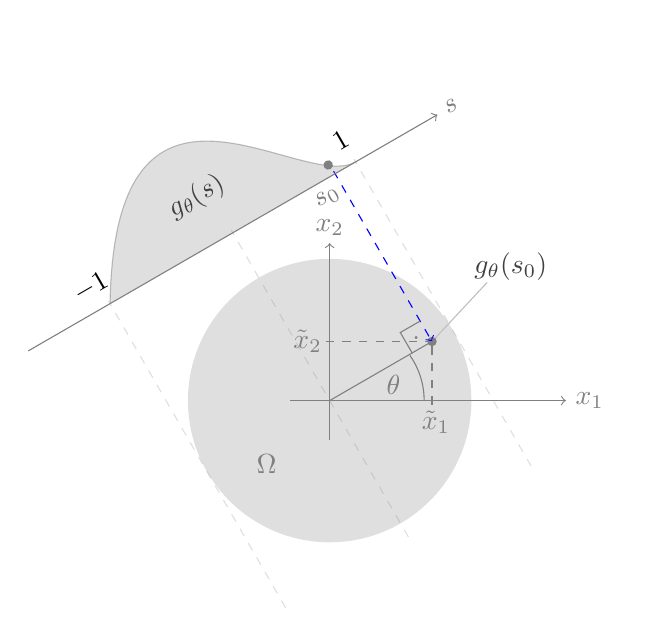
\begin{tikzpicture}	
	\fill[nearly transparent, color=gray] (0,0) circle (1.8cm);
	
	\draw [gray] [->](-0.5,0) -- (3,0); % x-Achse
	\draw [gray] (3, 0) node [right] {$x_1$};
	
	\draw [gray] [->](0,-0.5) -- (0,2); % y-Achse
	\draw [gray] (0, 2.2) node {$x_2$};
	
	\draw[lightgray](1.3,0.75) -- (2, 1.5);
	\fill[gray](1.3,0.75) circle [radius=0.06]; % ein Punkt		
	\draw [darkgray] (2.3, 1.7) node {$g_{\theta}(s_0)$};
	
	\draw [rotate=30, xshift=1.5cm, ->, dashed] [blue] (0,2.5) -- (0,0); % strahl
			
	
	\draw [xshift=1.05cm, yshift=0.6cm, rotate=120, - ] [gray] (0,0) -- (0.3,0);
	\draw [xshift=0.89cm, yshift=0.86cm, rotate=30, - ] [gray] (0,0) -- (0.3,0);
	\draw [gray] (1.1, 0.8)  node {$.$};
	
	\draw [rotate=30] [gray] [-] (0,0) -- (1.5, 0);
	
	\draw [dashed] [gray] (1.3,-0.05) -- (1.3,0.75); % x-Projektion
	\draw [gray] (1.35,-0.28)  node {$\tilde{x}_1$};
	
	\draw [dashed] [gray] (-0.05,0.75) -- (1.3,0.75); % y-Projektion		
	\draw [gray] (-0.28,0.75)  node {$\tilde{x}_2$};
	
	\draw [lightgray] [rotate=30, yshift=70] (-1.8,0) .. controls (0,3) and (1,0) .. (1.8,0);
	\fill [nearly transparent, color=gray] [rotate=30, yshift=70] (-1.8,0) .. controls (0,3) and (1,0) .. (1.8,0);

	\fill[ rotate=30, xshift=0.18cm, yshift=1.85cm, gray](1.3,0.75) circle [radius=0.06]; % ein Punkt
	
	\draw [rotate=30, xshift=0, yshift=70] [gray] [->] (-3,0) -- (3, 0);
	\draw [gray] (3.7, 0)  node [rotate=30, xshift=0, yshift=123] {$s$};
	
	\draw [gray] (0, 0)  node [rotate=30, xshift=1.55cm, yshift=2.25cm, left] {$s_0$};
	
	\draw [darkgray] (-0.2, 0)  node [rotate=30, yshift=85] {$g_{\theta}(s)$};		
	
	\draw [rotate=30, xshift=0cm, dashed] [nearly transparent, color=gray] (0,-2) -- (0,2.5); % punktiert Mitte
	\draw [rotate=30, xshift=1.8cm, dashed] [nearly transparent, color=gray] (0,-2) -- (0,2.5); % rechts punktiert
	\draw [rotate=30, xshift=-1.8cm, dashed] [nearly transparent, color=gray] (0,-2) -- (0,2.5); % links punktiert 
	
	\draw  (-1.8, 0) node [left, rotate=30, yshift=53]  {$-1$};
	\draw  (1.8, 0) node [right, rotate=30, yshift=105]  {$1$};
	
	\draw [gray] (1.2,0) arc [start angle=0, end angle=35, radius=1cm];
	\draw [gray] (0.6, 0.2) node [right] {$\theta$};
	
	\draw [gray] (-0.8, -0.8) node {$\Omega$};
	
	\end{tikzpicture}
	\caption{Ein Beispiel der Rückprojektion eines Projektionswerts $g_{\theta}(s_0)$ auf einen Punkt $x \in \Omega$. Mit $g_{\theta}(s)$ ist hier eine Projektion bei einem festen Winkel $\theta$ bezeichnet, also $g_{\theta}(s) = g(s,\theta)$.}
	\label{fig:1.7}
\end{figure}	  
\begin{proof}[Beweis von Lemma \ref{lemma:2}.]
Seien $f \in L^2(\Omega)$ und $g \in L^2(Z)$ beliebig, dann gilt
\begin{equation}
	\begin{split}
		\langle \mathcal{R} f, g \rangle_{L^2(Z)} & = \int\limits_{Z}^{} \left( \mathcal{R} f(s,\theta) \right) g(x^{T}\omega(\theta),\theta) \ \mbox{d}s \mbox{d}\theta \\
		& \stackrel{(\ref{equa:1.10})}{=} \int\limits_{0}^{\pi} \int\limits_{-1}^{1} \left( \int\limits_{-\gamma(s)}^{\gamma(s)}f(s\omega(\theta) + t\omega^{\perp}(\theta)) \mbox{d}t  \right) g(x^{T}\omega(\theta),\theta) \ \mbox{d}s \ \mbox{d}\theta.
		\end{split}
	\label{equa:1.23}
\end{equation}
An dieser Stelle machen wir eine Substitution in der rechten Seite von (\ref{equa:1.23}). Hier nutzen wir (\ref{equa:1.22}) aus und schreiben $x^T \omega(\theta) = \omega^T(\theta)x = s$. Dann bekommt man $g(x^{T}\omega(\theta),\theta) = g(\omega^T(\theta)x,\theta)$ und wir wollen die Funktion $f$ im Punkt $x$ betrachten, also $f(s\omega(\theta) + t\omega^{\perp}(\theta)) = f(x)$. Somit erhalten wir einen Integrationsbereich über $\Omega$. Nun führen wir (\ref{equa:1.24}) weiter:
\begin{equation}
	\begin{split}
		\langle \mathcal{R} f, g \rangle_{L^2(Z)} & = \int\limits_{0}^{\pi} \int\limits_{-1}^{1} \left( \int\limits_{-\gamma(s)}^{\gamma(s)}f(s\omega(\theta) + t\omega^{\perp}(\theta)) \mbox{d}t  \right) g(x^{T}\omega(\theta),\theta) \ \mbox{d}s \ \mbox{d}\theta \\
		& \stackrel{\mbox{\scriptsize Subst.}}{=}  \int\limits_{0}^{\pi} \left( \int\limits_{-1}^{1} \int\limits_{-\gamma(s)}^{\gamma(s)}f(x) g(\omega^T(\theta)x,\theta) \ \mbox{d}t \ \mbox{d}s \right) \mbox{d}\theta \\	
		& = \int\limits_{0}^{\pi} \int\limits_{\Omega} f(x) g(\omega^T(\theta)x,\theta) \ \mbox{d}x \ \mbox{d}\theta \\
		& = \int\limits_{\Omega} f(x) \left( \int\limits_{0}^{\pi} g(\omega^T(\theta)x,\theta) \ \mbox{d}\theta \right) \mbox{d}x  \\  
		& =\langle f, \mathcal{R^*} g \rangle_{L^2(\Omega)}.
	\end{split}
	\label{equa:1.24}
\end{equation}	 
Somit ist $\mathcal{R^*}$ adjungierter Operator der Radon Transformation und ist nach Satz von Schauder auch kompakt, wenn $\mathcal{R}$ kompakt ist. (\cite[S. 185]{Heuser75}).	 
\end{proof}

\subsubsection{Kompaktheit von $\mathcal{R}$}

Um die Kompaktheit von $\mathcal{R}$ zeigen zu können, werden wir an dieser Stelle einen Umweg einschlagen. Dafür ziehen wir ein Ergebnis aus \cite[S. 45]{Rieder03} heran. Es handelt sich um einen zu $\mathcal{R}$ adjungierten Operator $\tilde{\mathcal{R}}^*$ folgender Gestalt:
\begin{equation}
	\tilde{\mathcal{R}}^* : L^2(Z, \frac{1}{\gamma(s)}) \rightarrow L^2(\Omega).
	\label{equa:1.25}
\end{equation}
Hier wurde $\gamma(s)$ im Sinne der Gleichung (\ref{equa:1.8}) benutzt. Und der Raum $L^2(Z,\frac{1}{\gamma(s)})$ ist mit dem folgenden Skalarprodukt versehen
\begin{equation}
	\langle g,f \rangle = \int\limits_{Z} g \overline{f}\frac{1}{\gamma(s)}\mbox{d}s \mbox{d}\theta.
	\label{equa:1.26}
\end{equation}

Wir können festhalten dass der Operator $\mathcal{R'}:L^2(\Omega) \rightarrow  L^2(Z, \frac{1}{\gamma(s)})$ kompakt ist\footnote{Prinzipiell sind $\mathcal{R}$ und $\mathcal{R'}$ gleich, es ist derselbe Operator, der aber $L^2(\Omega)$ in einen anderen Raum abbildet. Die Bezeichnung $\mathcal{R}'$ führen wir ein, um uns Verwechslungen zu ersparen.}. Die Kompaktheit folgt eben aus der SWZ von $\mathcal{R}'$. Denn die Singulärwerte von $\mathcal{R}'$
\[
\sigma_j = 2\sqrt{\frac{\pi}{j + 1}}, \ \ j \in \N
\]
bilden eine Nullfolge, was nach einer längeren Rechnung aus \cite[S. 43]{Rieder03} folgt. Also schreiben wir $\mathcal{R}' \in \mathscr{K}(L^2(\Omega), L^2(Z,\frac{1}{\gamma(s)}))$\footnote{\label{foot:7}$\mathscr{K}(X,Y) = \{ A \in \mathscr{L}(X,Y) \ | \ A \mbox{ ist kompakt } \}$ }. 

Wir veranschaulichen die entstandene Situation in einem kommutativen Diagramm  
\begin{equation}
	\begin{xy}
	\xymatrix{
		L^2(\Omega) \ar[rr]^{\mathcal{R}} \ar@<2pt>[rd]^{\mathcal{R}'} &  & L^2(Z)\\
		&  L^2(Z, \frac{1}{\gamma(s)}) \ar@<2pt>[lu]^{\tilde{\mathcal{R}}^*} \ar[ru]_{\mbox{Id}}&
		}
	\end{xy}
	\label{equa:1.27}
\end{equation}
und stellen fest, dass $\mathcal{R}$ als eine Komposition zweier Abbildungen darstellbar ist. Hier bedeutet $\mbox{Id}$ die Identität auf $L^2(Z)$ dar. Der Unterschied zwischen $L^2(Z)$ und $L^2(Z,\frac{1}{\gamma(s)})$ besteht nur in der Definition des Skalarprodukts auf diesen beiden Räumen.

Insgesamt würde es heißen, dass wir die Komposition $\mbox{Id}\circ\mathcal{R}' = \mathcal{R}$ bezüglich der Kompaktheit beurteilen müssen. Dafür wird uns ein nützlicher Satz aus \cite[S. 27]{Rieder03} gute Dienste leisten (ohne Beweis) :
\begin{theorem}
	Seien $X, Y$ und $Z$ normierte Räume. Falls $A \in \mathscr{L}(X,Y)$ und $B \in \mathscr{K}(Y,Z)$ oder $A \in \mathscr{K}(X,Y)$ und $B \in \mathscr{L}(Y,Z)$, dann gilt $BA \in \mathscr{K}(X,Z)$.
	\label{satz:1}
\end{theorem}
Somit wollen wir zeigen, dass der Operator $\mbox{Id}:L^2(Z, \frac{1}{\gamma(s)}) \rightarrow L^2(Z)$ beschränkt ist, und somit auch stetig ist. Danach könnten wir den Satz \ref{satz:1} benutzen, um die Kompaktheit von $\mathcal{R}$ zu zeigen.

Sei nun $g(s,\theta) \in L^2(Z)$ beliebig, dann können wir folgende Abschätzung durchführen:
\begin{equation}
	\begin{split}
		\parallel \mbox{Id} \ g(s, \theta) \parallel_{L^2(Z)}^{2} & = \ \int \limits_{Z} |\mathcal{R}f(s, \theta)|^2 \mbox{d}s \mbox{d}\theta \\
		& \stackrel{(\ref{equa:1.26})}{\leq} \int \limits_{Z}  |\mathcal{R}f(s, \theta)|^2 \frac{1}{\gamma(s)} \ \mbox{d}s \ \mbox{d}\theta\\
		& = \ \parallel g(s, \theta) \parallel_{L^2(Z, \frac{1}{\gamma(s)})}^{2}.
	\end{split}
	\label{equa:1.28}
\end{equation}
Die letzte Abschätzung beruht auf der Kenntnis, dass  $\gamma(s) \leq 1$ für alle $s \in (-1,1)$, somit aber $\frac{1}{\gamma(s)} \geq 1$ gilt. Nun haben wir gezeigt, dass $\parallel \mbox{Id} \parallel_2 \leq 1$ beschränkt und demnach stetig ist. Also gilt $\mbox{Id} \in \mathscr{L}(L^2(Z, \frac{1}{\gamma(s)}), L^2(Z))$. Dieses Ergebnis ist für uns ausreichend um den Satz \ref{satz:1} benutzen zu können, d.h 
\begin{equation}
	\mathcal{R} \stackrel{(\ref{equa:1.27})}{=} \mbox{Id} \circ \mathcal{R}' \xLongrightarrow{\text{Satz \ref{satz:1}}} \mathcal{R} \in \mathscr{K}(L^2(\Omega), L^2(Z)).
	\label{equa:1.29}
\end{equation}

Nun sind wir am Ende dieses Kapitels angelangt und nach einigen Untersuchungen können wir festhalten, dass der lineare stetige Operator $\mathcal{R} : L^2(\Omega) \rightarrow L^2(Z)$ kompakt ist und einen kompakten adjungierten Operator $\mathcal{R^*}$ hat. Diese Ergebnisse spielen eine zentrale Rolle bei der Singulärwertzerlegung (SWZ) eines kompakten Operators und beleuchten das Problem der Invertierung solcher Operatoren sehr gut.

\subsubsection{Die Singulärwertzerlegung (SWZ) von $\mathcal{R}$}

Im Folgenden wird die allgemeine Form der SWZ des Operators $\mathcal{R}$ angegeben, eine konkrete wird in \cite[Kap. 2.5]{Rieder03} hergeleitet, jedoch aber nur für $\mathcal{R}'$. Um zu SWZ von $\mathcal{R}$ zu gelangen, ermittelt man zuerst die Eigenwerte und Eigenvektoren von $\mathcal{R}\mathcal{R^*} : L^2(Z) \rightarrow L^2(Z)$, die als Komposition kompakter Operatoren kompakt ist. Demnach gilt der \textit{Spektralsatz für selbstadjungierte kompakte Operatoren} \cite[S. 30]{Rieder03} und man bekommt 
\begin{equation}
	\mathcal{R}\mathcal{R^*}g = \sum\limits_{j=1}^{\infty} \lambda_j \langle g, v_j \rangle_{L^2(Z)} v_j, \ \ \mbox{für alle} \ \ g \in L^2(Z).
	\label{equa:1.30}
\end{equation}
Hier bildet $\{ \lambda_j \}_{j \in \N} \in \R$ eine Folge mit der absteigenden Anordnung der Eigenwerte $|\lambda_1| \geq |\lambda_2| \geq ... > 0$ und $\{ v_j\}_{j \in \N} \in L^2(Z)$ ein Orthonormalsystem in $\mbox{Kern}(\mathcal{R})^{\perp}$. Eine wichtige Tatsache ist, dass die Folge $\{\lambda_j\}_{j \in \N}$ entweder abbricht oder gegen Null konvergiert.

Die Singulärwerte und das Orthonormalsystem $\{u_j\}_{j \in \N}$ des Bildes von $\mathcal{R}$ bekommen wir aus
\begin{equation}
	\begin{split}
		(i). \ \sigma_j &:= \sqrt{\lambda_j}\\ 
		(ii). \ u_j	&:= \sigma_j^{-1}\mathcal{R}v_j
	\end{split}
	 , \ \  j \in \N.
	 \label{equa:1.31}
\end{equation}
Mit den Ergebnissen aus (\ref{equa:1.30}) und (\ref{equa:1.31}) kann nun die SWZ der Radon Transformation angegeben werden
\begin{equation}
	\mathcal{R}f = \sum\limits_{j = 1}^{\infty} \sigma_j \langle f, v_j\rangle_{L^2(\Omega)} u_j.
	\label{equa:1.32}
\end{equation}
Das Tripel $\{(\sigma_j, v_j, u_j)\}$ nennt man \textit{Singulärsystem} eines kompakten Operators und die Folgen $\{u_j\}_{j \in \N}$ und $\{ v_j\}_{j \in \N}$ bilden folgende Orthonormalsysteme
\begin{equation}
	\overline{\mbox{Span}\{u_j | j \in \N \} } = \overline{\mbox{Bild}(\mathcal{R})} \ \ \mbox{und} \ \ \overline{\mbox{Span}\{v_j | j \in \N \} } = \mbox{Kern}(\mathcal{R})^{\perp}.
	\label{equa:1.33}
\end{equation}

Die Gleichung (\ref{equa:1.32}) wird im nächsten Kapitel bei der Klärung des Begriffs \textit{schlecht gestellter Probleme} sehr hilfreich sein. 








%\chapter{Das inverse Problem}
\label{cha:2}

In diesem Abschnitt soll der Bezug der Bildrekonstruktion aus CT-Daten zum Begriff \textit{inverser Probleme} hergestellt und der Frage nachgegangen werden, warum inverse Probleme meist schlecht gestellt seien. 

Zunächst können wir festhalten, dass in allen naturwissenschaftlichen Fragestellungen, die Wirkungen von den Ursachen herbei geführt werden. Dies ist eine Kausalität, welche sich in einem mathematischen Modell beschreiben lässt. Anlehnend an \cite[S. 14]{Rieder03} definieren wir ein mathematisches Modell, wie folgt

\begin{Definition}
	Ein \textbf{mathematisches Modell} ist eine Abbildung
	\[A: X \rightarrow Y\]
	von der Menge der Ursachen (Parameter) $X$ in die Menge der Wirkungen (Daten) $Y$. Im Falle des \textbf{inversen Problems} wird zu einer Wirkung $y \in Y$ die Ursache $x \in X$ gesucht, sodass $Ax = y$ erfüllt ist. Umgekehrt liegt ein \textbf{direktes Problem} vor.
	\label{def:3}
\end{Definition}
Jetzt ist es klar, warum Bildrekonstruktion aus CT-Daten zu den inversen Problemen gehört. Man möchte aus der Menge der Projektionsdaten $(Y)$ die unbekannte Dichteverteilung $(X)$ des bestrahlten Materials berechnen.

Im nächsten Schritt soll geklärt werden, was ein \textit{schlecht gestelltes} Problem ist. Dazu betrachten wir die Definition aus \cite[S. 24]{Rieder03}
\begin{Definition}
	Sei $A:X \rightarrow Y$ eine Abbildung zwischen Hilberträumen $X$ und $Y$. Das Problem $(A, X, Y)$ heißt \textbf{schlecht gestellt nach Nashed}\cite{Nashed} (ill-posed), wenn das Bild von $A$ nicht abgeschlossen ist. Ansonsten heißt das Problem $(A,X,Y)$ \textbf{gut gestellt nach Nashed}.	
	\label{def.4}
\end{Definition}
Nun ist es an der Zeit, die erarbeiteten Ergebnisse aus dem Kapitel (\ref{cha:1.1}) heranzuziehen. Entsprechend der Definition \ref{def.4}. schreiben wir den Ausdruck (\ref{equa:1.10}) als $(\mathcal{R}, L^2(\Omega), L^2(Z))$ um. Somit ist ein schlecht gestelltes Problem gegeben, welches durch die SWZ (\ref{equa:1.32}) des Operators $\mathcal{R}$
 
\[ \mathcal{R}f = \sum\limits_{j = 1}^{\infty} \sigma_j \langle f, v_j\rangle_{L^2(\Omega)} u_j. \]  

einzusehen ist. Man erkennt, dass das Bild des Operators $\mathcal{R}$ nicht abgeschlossen ist.

Wir wollen nun den Operator $\mathcal{R}$ invertieren. Aus dem \textit{Spektralsatz für selbstadjungierte kompakte Operatoren} \cite[S. 30]{Rieder03} folgt, dass die Eigenwerte von $\mathcal{R}\mathcal{R^*}$ der Bedingung

\[ \forall j \in \N : \lambda_j > 0 \ \ \mbox{und} \ \ \lambda_j \xrightarrow[{j \rightarrow \infty}]{} 0 \]

genügen. Entsprechend (\ref{equa:1.31}, $(i)$) sind die Singulärwerte von $\mathcal{R}$ alle größer Null. Dies erlaubt die Invertierung der Gleichung (\ref{equa:1.32}) und wir schreiben
\begin{equation}
	\mathcal{R}^{+}g = \sum\limits_{j = 1}^{\infty} \sigma_j^{-1} \langle g, u_j \rangle_{L^2(Z)} v_j \ \ \mbox{für} \ \ g \in \mbox{Bild}(\mathcal{R}).
	\label{equa:2.1}
\end{equation}
Aus der Gleichung (\ref{equa:2.1}) ist zu erkennen, dass der Ausdruck $\sigma_j^{-1}$ für  $j \rightarrow \infty$ gegen Unendlich läuft und somit ist $\mathcal{R}^{+}$ nicht beschränkt, was also die Nichtstetigkeit bedeutet. 

Die Bezeichnung $\mathcal{R}^{+}$ nennt man \textit{verallgemeinerte Inverse} des kompakten Operators $\mathcal{R}$ und wir bestätigen die obige Überlegung mit folgendem Satz, dessen Beweis in \cite[S. 32]{Rieder03} nachgelesen werden kann.
\begin{theorem}
	Sei $A : X \rightarrow Y$ ein kompakter Operator mit einem Singulärsystem $\{(\sigma_j, v_j, u_j)\}$. Dann ist die verallgemeinerte Inverse durch
	\[ A^{+} g  = \sum\limits_{j = 1}^{\infty} \sigma_j^{-1} \langle g, u_j \rangle_Y v_j \ \ \ f\ddot{u}r \ \ g \in \mathcal{D}_A \footnote{\label{foot:8}$\mathcal{D}_A$ : Definitionsbereich der Abbildung $A : X \rightarrow Y$.} \]
	gegeben. Hat $A$ ein endlichdimensionales Bild, dann ist $A^+$ stetig.   
	\label{satz:2}
\end{theorem}
Im Falle des Operators $\mathcal{R} : L^2(\Omega) \rightarrow L^2(Z)$ ist das Bild \textit{unendlichdimensional}, was auch dem Ausdruck (\ref{equa:1.32}) anzusehen ist. 

Gemäß obigen Überlegungen ist das Problem rein theoretisch. In der Praxis hängt die Radon Transformation nur von endlich vielen Argumenten ab, also von $s_i$ mit $i \in [1,k], \ k \in \N$ und  von $\theta_l$ mit $l \in [1,q], \ q \in \N$. Damit ist gemeint, dass man gerade $n = kq$ Projektionen erzeugen kann. Somit bekommen wir
\begin{equation}
	\mathcal{R}f = \sum\limits_{j = 1}^{n} \sigma_j \langle f, v_j\rangle_{L^2(\Omega)} u_j, \ \ n \in \N.
	\label{equa:2.2}
\end{equation}
\begin{Bemerkung}
	An dieser Stelle lassen wir die Diskretisierungstheorie unendlichdimensionaler Operatoren bei Seite. Wir verweisen hier auf \cite[S. 153]{Rieder03}. Zu erwähnen ist, dass $n \in \N$ in (\ref{equa:2.2}) nicht die ersten $n$ Eigenvektoren bezeichnet, sondern, dass die unendliche Dimension von $\mathcal{R}$ auf $n$-Dimensionalität interpoliert wurde.
	\label{bem:4}
\end{Bemerkung}
\begin{Bemerkung}
	Die Elemente $\mathcal{R}$, $f$, $\sigma_j$, $v_j$ und $u_j$ in (\ref{equa:2.2}) sind nicht mit denen aus (\ref{equa:1.32}) zu verwechseln. In diesem Falle sind es die diskretisierte Elemente.
	\label{bem:5}
\end{Bemerkung}
Wir bilden zuerst die Inverse $\mathcal{R}^{+}$ von $\mathcal{R}$ und diskutieren das Verhalten einzelner Summenglieder von
\begin{equation}
	\mathcal{R}^{+} g  = \sum\limits_{j = 1}^{n} \sigma_j^{-1} \langle g, u_j \rangle_{L^2(Z)} v_j.
	\label{equa:2.3}
\end{equation}
Hier stellt $g$ eine reale Messung der Projektionen dar, bei der gewisse Messungenauigkeiten anzunehmen sind. Diese Messungenauigkeiten werden mit steigendem $j$ um dem Faktor $\sigma_j^{-1}$ in Richtung des Eigenvektors $u_j$ verstärkt. Anderes ausgedrückt, wird auf diese Weise rekonstruierte Lösung $\mathcal{R}^{+} g$ immer verschwommener, was auf die Oszillation der Eigenvektoren zurückzuführen ist.

Im Allgemeinen bedarf es einer Bedingung an die Koeffizienten $\langle g, u_j \rangle_{L^2(Z)}$, die besagt, dass sie schnell genug abfallen müssen, um nicht von $\sigma_j^{-1}$ ins Unendliche geschickt zu werden. Genau das besagt die \textit{Picard-Bedingung} (s.a. \cite[S. 31]{Rieder03}).
\begin{theorem}[\textit{\textbf{Picard-Bedingung}}]
	Seien $X, Y$ Hilberträume und $A : X \rightarrow Y$ ein kompakter Operator mit einem singulärem System $\{(\sigma_j, v_j, u_j)\}$. Die Reihe 
	\begin{equation}
		\sum\limits_{j=1}^{\infty} \frac{|\langle g, u_j \rangle_Y|^2}{\sigma_j^2}
		\label{equa:2.4}
	\end{equation}
	konvergiert genau dann, wenn $g \in \mbox{Bild}(A)$.
	\label{satz:3}
\end{theorem}
Die verrauschten Messdaten liegen nie in dem Bild der Radon Transformation. Deshalb werden die Anteile der Lösung mit kleinen Singulärwerten (oder hochfrequente Anteile) mit speziellen Techniken \textit{gedämpft}, so dass die Reihe (\ref{equa:2.4}) konvergiert. Die Dämpfung hochfrequenter Anteile nennt man im Allgemeinen Regularisierung eines schlecht gestellten Problems. Die Art der Regularisierung unterliegt dem Rekonstruktionsverfahren. Das aber, wird das Hauptthema des nächsten Kapitels sein. 






%\chapter{Rekonstruktionsverfahren und ihre Implementierung}
\label{cha:3}

In diesem Kapitel werden wir die praktische Vorgehensweise einiger Bildrekonstruktionstechniken in der Computertomographie diskutieren. Den Stützpunkt folgender Diskussion werden wir zuerst hier festigen. Dazu schauen wir uns nochmal das diskrete Modell (\ref{equa:2.2}) an:

\[\mathcal{R}f = \sum\limits_{j = 1}^{n} \sigma_j \langle f, v_j\rangle_{L^2(\Omega)} u_j, \ \ n \in \N.\] 

Die obige Gleichung stellt genau $n$ Projektionen $p \in \R^n$ einer unbekannten Dichtefunktion $f \in \R^m$ dar. Die Anzahl der Projektionen $n$ setzt sich aus der Anzahl der Detektorzellen $k \in  \N$ im Detektorband und der Anzahl der Winkel $q \in \N$ zu denen die Projektionen erzeugt worden sind zusammen. Insgesamt ergibt sich
\begin{equation}
	n = kq \ \ \mbox{für} \ n,k,q \in \N.
	\label{equa:3.1}
\end{equation}
\begin{figure}[H]
	\centering
	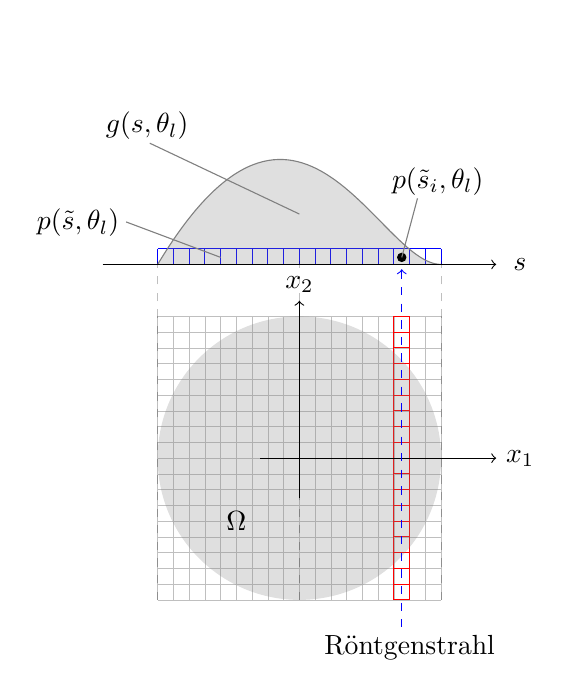
\begin{tikzpicture}
	
	\draw [step=0.2,blue, thin, rotate=0, xshift=0, yshift=70] (-1.8,0) grid (1.8,0.2); % detector grid
	
	\draw [step=0.2, lightgray, very thin] (-1.8,-1.8) grid (1.8,1.8); % picture grid
	
	\draw [step=0.2, red, thin, rotate=0, xshift=1.2cm, yshift=0] (0,-1.8) grid (0.2,1.8);
	
	\fill[nearly transparent, color=gray] (0,0) circle (1.8cm);
	
	\draw [black] [->](-0.5,0) -- (2.5,0); % x-Achse
	\draw [black] (2.5, 0) node [right] {$x_1$};
	
	\draw [black] [->](0,-0.5) -- (0,2); % y-Achse
	\draw [black] (0, 2.2) node {$x_2$};
	
	\draw [rotate=0, xshift=1.3cm, <-, dashed] [blue] (0,2.4) -- (0,-2.2); % strahl
	\draw [black] (1.4, -2.4) node {Röntgenstrahl};
	
	\draw [gray] [rotate=0, yshift=70] (-1.8,0) .. controls (0,3) and (1,0) .. (1.8,0);
	\fill [nearly transparent, color=gray] [rotate=0, yshift=70] (-1.8,0) .. controls (0,3) and (1,0) .. (1.8,0);
	
	\fill[ rotate=0, xshift=0cm, yshift=1.8cm, black](1.3,0.75) circle [radius=0.06]; % ein Punkt
	
	\draw [rotate=0, xshift=0, yshift=70] [black] [->] (-2.5,0) -- (2.5, 0);
	\draw [black] (2.8, 0)  node [rotate=0, xshift=0, yshift=70] {$s$};
	
	\draw [black] (0, 0)  node [rotate=0, xshift=-80, yshift=85] {$p(\tilde{s}, \theta_l)$};
	\draw[gray,  yshift=1.8cm](-1,0.75) -- (-2.2, 1.2);	
	
	\draw [black] (0, 0)  node [rotate=0, xshift=50, yshift=100] {$p(\tilde{s}_i, \theta_l)$};
	\draw[gray,  yshift=1.8cm](1.3,0.75) -- (1.5, 1.5);		
	
	\draw [black] (0, 0)  node [rotate=0, xshift=-55, yshift=120] {$g(s, \theta_l)$};
	\draw[gray,  yshift=1.8cm](0,1.3) -- (-1.9, 2.2);		
	
	\draw [rotate=0, xshift=0cm, dashed] [nearly transparent, color=black] (0,-1.8) -- (0,2.5); % punktiert Mitte
	\draw [rotate=0, xshift=1.8cm, dashed] [nearly transparent, color=black] (0,-1.8) -- (0,2.5); % rechts punktiert
	\draw [rotate=0, xshift=-1.8cm, dashed] [nearly transparent, color=black] (0,-1.8) -- (0,2.5); % links punktiert 
	
	\draw [black] (-0.8, -0.8) node {$\Omega$};
	
	\end{tikzpicture}
	\caption{Anschauliche Darstellung der Diskretisierung der Dichtefunktion $f$. Entlang des Röntgenstrahls (alle rot umrandeten Pixel) an der Stelle $s_i$ und zu einem festen Winkel $\theta_l = 0$, werden die Werte von $f$ zu dem Wert $p(\tilde{s}_i, \theta_l)$ aufsummiert. $p(\tilde{s}, \theta_l)$ ist der Vektor zu allen Strahlen an den Stellen $\tilde{s}_i$ und somit die Diskretisierung von $g(s,\theta_l)$.}
	\label{fig:3.1}
\end{figure}
Die Diskretisierung von $f$ hängt hingegen nur von der Anzahl der Detektorzellen $k \in \N$ im Detektorband ab. Betrachtet man die Abbildung \ref{fig:3.1}, dann wird man erkennen, dass die $k$ Detektorzellen die Breite und die Höhe des zu rekonstruierenden Bildes $f$ festlegen, demnach ergibt sich
\begin{equation}
	m = k^2 \ \ \mbox{für} \ k, m \in \N.
	\label{equa:3.2}
\end{equation}
\begin{Bemerkung}
	Praktisch gesehen, stellt $k$ die Anzahl der digitalen Pixel in der Breite und Tiefe eines digitalen Bildes $f$ dar.
	\label{bem:6}
\end{Bemerkung}
Bevor wir im nächsten Schritt zur Bildrekonstruktion übergehen, schauen wir uns zuerst die Entstehung der Projektionsdaten aus der Radon Transformation etwas genauer an. Betrachten wir dazu die Gleichung (\ref{equa:1.10}) und die Abbildung \ref{fig:1.6}.
\[ \mathcal{R}f(s,\theta) = \int\limits_{-\gamma(s)}^{\gamma(s)} f(s\omega(\theta) + t\omega^{\perp}(\theta))\mbox{d}t. \]
Im diskreten Fall $\tilde{f} \in \R^{k \times k}$ wird man feststellen, dass (\ref{equa:1.10}) die Summe aller Werte von $\tilde{f}$ entlang einer Geraden $G$, den Projektionswert $p(\tilde{s}_i, \theta_l)$ an der Stelle $\tilde{s}_i, i \in [1,k]$, entsprechend dem Winkel $\theta_l, \ l \in [1,q] $, liefert. Damit kann (\ref{equa:1.10}) für die Transformation eines digitalen Bildes folgendermaßen interpretiert werden
\begin{equation}
	\begin{split}
		p(\tilde{s}_i, \theta_l) & = \sum \limits_{j = 1}^{m} \mu_j \Delta\tilde{t}, \ \mbox{mit} \ m = k^2, \\
		\mbox{für} \ \mu_j & = \left\{ \begin{matrix}
							\tilde{f}_j & : & \mbox{falls } \tilde{f}_j\cap G \neq \emptyset \\ 
							0 & : & \mbox{sonst}
						\end{matrix}.\right.
	\end{split}
	\label{equa:3.3}
\end{equation}

Fasst man auf diese Weise zu jedem $\tilde{s}_i$ (wobei $\Delta\tilde{t} = 1$) die entsprechende Werte von $\tilde{f}$ zusammen, so entsteht der Projektionsvektor $p(\tilde{s},\theta_l)$ (Abb. \ref{fig:3.1}). Stellt man alle Projektionen $p(\tilde{s}, \theta_l)$ entsprechend der Winkelreihenfolge $\theta_l, \ l \in [1,q]$ auf, so entsteht ein digitales Bild der Projektionsdaten der diskreten Radon Transformation.
\begin{Bemerkung}
	Die Gleichung (\ref{equa:3.3}) entspricht der Parallelstrahlengeometrie. Das bedeutet, dass alle Geraden $G$, die das Objekt durchdringen, parallel zueinander sind. Um (\ref{equa:3.3}) in die Fächerstrahlengeometrie zu überführen, müssen entsprechende geometrische Transformationen durchgeführt werden.
	\label{bem:7}
\end{Bemerkung}

Schauen wir uns ein konkretes Beispiel einer Radon Transformation an. Sei dazu die Abbildung \ref{fig:3.2} betrachtet. In Abb. \ref{fig:3.2.b} ist die Radontransformierte oder \textit{das Sinogramm} von Abb. \ref{fig:3.2.a} gemäß (\ref{equa:3.3}) zu sehen. Der Aufbau des Sinogramms entspricht dem oben beschriebenen Prinzip. Fasst man also das Sinogramm in Abb. \ref{fig:3.2.b} als eine Matrix auf, so ist jede Spalte der Matrix gleich einer Projektion $g(\tilde{s}, \theta_l)$ zu einem festem Winkel $\theta_l$. Die Implementierung der (diskreten) Radon Transformation ist im Abschnitt \ref{cha:A.1} kurz erläutert.
\begin{figure}[H]
	\begin{center}
		\subfloat[\label{fig:3.2.a}Phantombild]{{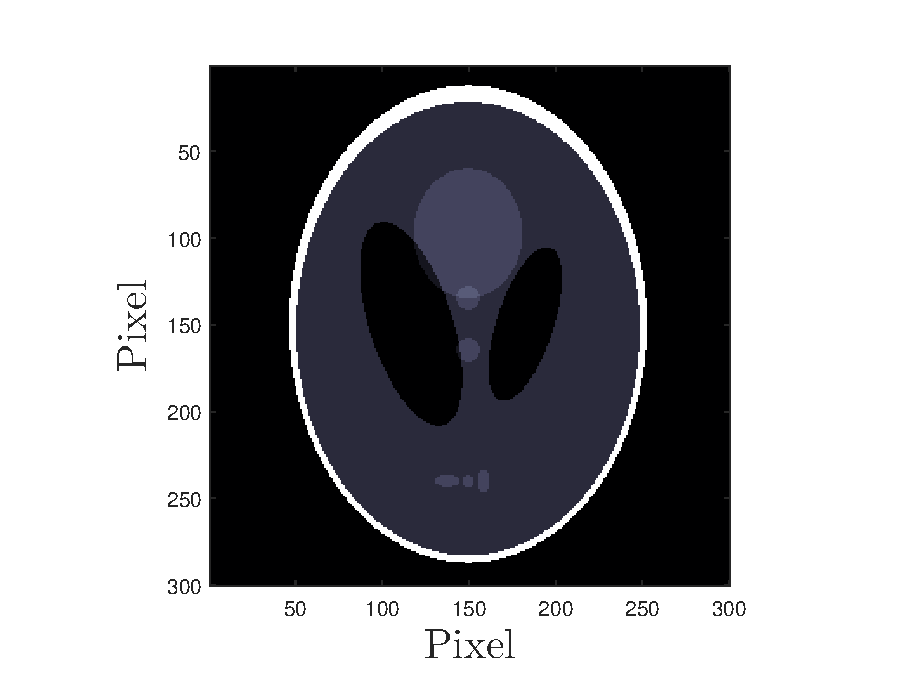
\includegraphics[width=0.5\textwidth]{phantom.eps} }}
		\subfloat[\label{fig:3.2.b}Die Radon Transformation des Phantombildes]{{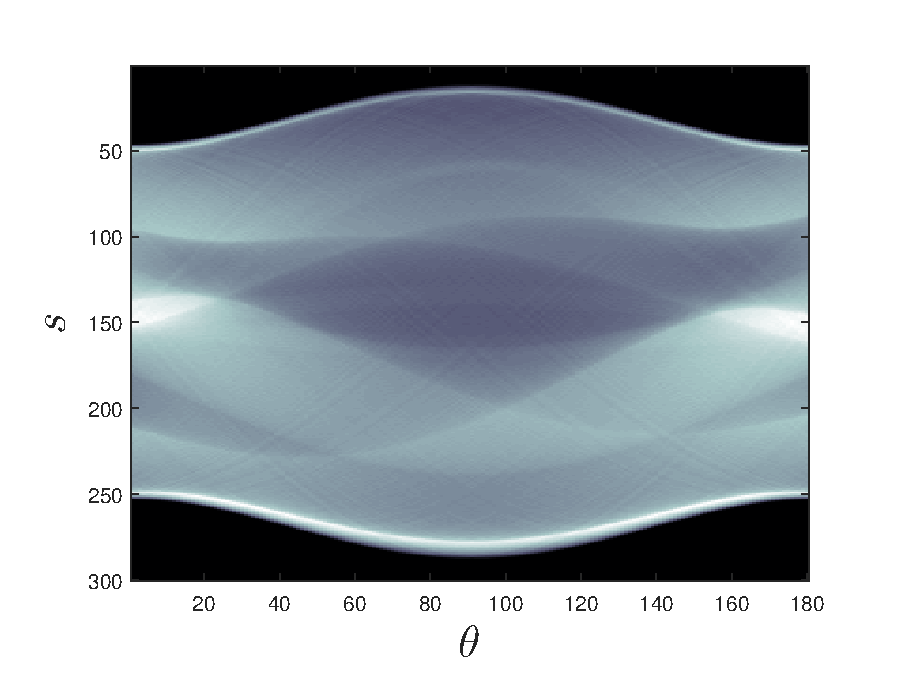
\includegraphics[width=0.5\textwidth]{rt_phantom.eps} }}
	\end{center}
	\caption{ Links (a) ist ein Phantombild (Quelle: \MATLAB, \texttt{\captionstring phantom(300)}) zu sehen, welches wir für alle Testzwecke in diesem Kapitel benutzen werden. Rechts (b) ist die Radontransformierte von (a) abgebildet. Die Transformation wurde über $\theta \in [0^{\circ}, 180^{\circ}]$ mit einer Schrittweite von $1^{\circ}$ durchgeführt. Das Detektorband hat eine Länge von $k = 300$, wobei $k$ gleich der Anzahl der Tiefenpixel von (a) ist. Somit bestimmt $k$ auch die Anzahl der Strahlen, die durch das Phantombild geschickt worden sind.}
	\label{fig:3.2}
\end{figure}

Sinogramme sind in der Praxis der computertomographischen Bildrekonstruktion genau die gemessenen Daten. Somit ist die Aufgabe das Bild des Ursprungsobjekts aus einem Sinogramm zu rekonstruieren. In folgenden Abschnitten werden wir uns vier solcher Rekonstruktionsverfahren anschauen. Dabei unterscheiden wir zwischen \textit{analytischen} und \textit{algebraischen} Verfahren. Als Nächstes wollen wir den Begriff der analytischen Rekonstruktion klären.

\section{Analytische Rekonstruktionsverfahren}
\label{cha:3.1}

Der Begriff der \textit{analytischen Rekonstruktion} bedeutet in diesem Fall, dass die Algorithmen der CT-Bildrekonstruktion direkt aus den analytischen Formeln hergeleitet werden. Solche Verfahren nutzen die Projektionsdaten zur Rekonstruktion des Bildes direkt aus. Zuerst schauen wir uns das einfachste davon an.

\subsection{Ungefilterte Rückprojektion}
\label{cha:3.1.1}

Den Ausgangspunkt dieses Abschnitts liefert uns der Adjungierte Operator (\ref{equa:1.21}). Schauen wir uns die Gleichung des Operators $\mathcal{R}^*$ noch einmal an: 

\[ \mathcal{R^*} g(x) = \int\limits_{0}^{\pi} \ g(x^{T}\omega(\theta),\theta) \mbox{d}\theta. \]  

Aus der Bemerkung \ref{bem:3} wissen wir bereits, dass (\ref{equa:1.21}) die ungefilterte Rückprojektion darstellt. Das Argument des Integranden in der obigen Gleichung ist ein fester Punkt $x$ der Kreisscheibe $\Omega$. Auf diesen Punkt $x$ wird aus allen Winkeln zurück projiziert. Führt man das für alle $x \in \Omega$ durch, so entsteht ein verschwommenes Bild des Originals, wie es die Abbildung \ref{fig:3.3.b} zeigt.
\begin{figure}[!h]
	\begin{center}
		\subfloat[\label{fig:3.3.a}Die Radon Transformation des Phantombildes aus Abb. \ref{fig:3.2.a}.]{{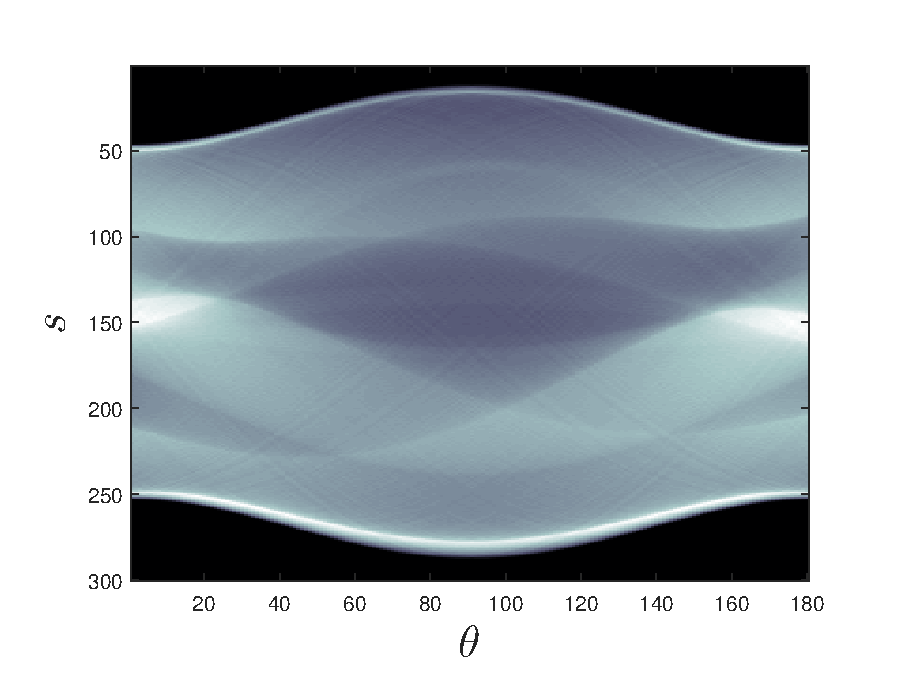
\includegraphics[width=0.5\textwidth]{rt_phantom.eps} }}
 		\subfloat[\label{fig:3.3.b}Ungefilterte Rückprojektion]{{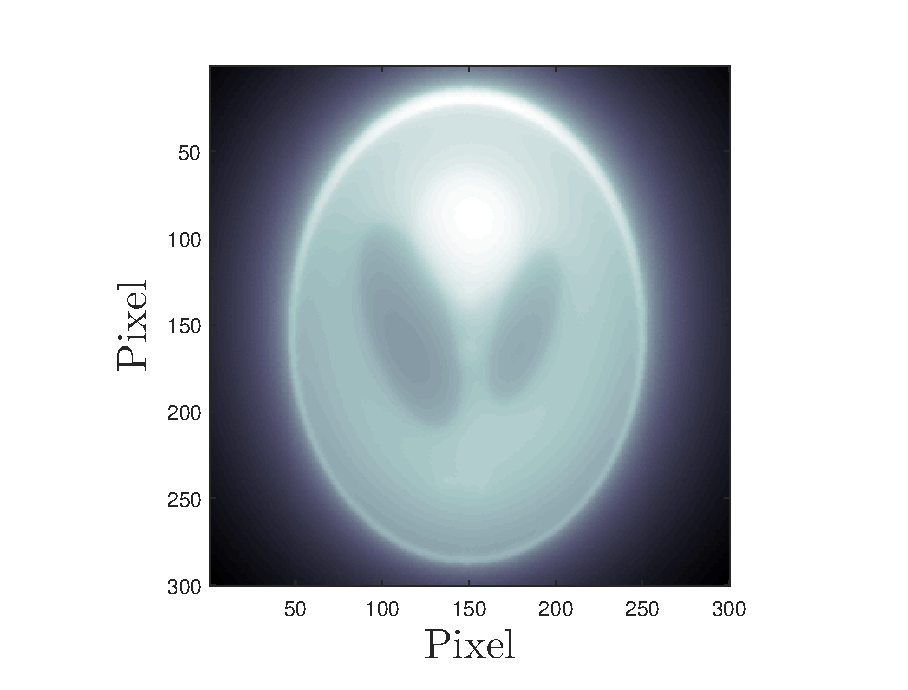
\includegraphics[width=0.5\textwidth]{backProjection.eps} }}
	\end{center}
	\caption{ Links (a) ist die Radontransformierte wie in der Abb. \ref{fig:3.2.b}. Rechts (b) ist die ungefilterte Rückprojektion von (b).}
	\label{fig:3.3}
\end{figure}

Jetzt wollen wir nachvollziehen, warum der Effekt der Verschwommenheit bei der ungefilterten Rückprojektion auftritt. Dazu sei zunächst die Abbildung \ref{fig:3.4} betrachtet, denn mit ihrer Hilfe können wir den Zusammenhang zweier Punkte in der Ebene $\Omega$ nachvollziehen.
\begin{figure}[H]
	\begin{minipage}[t]{0.4\textwidth}
		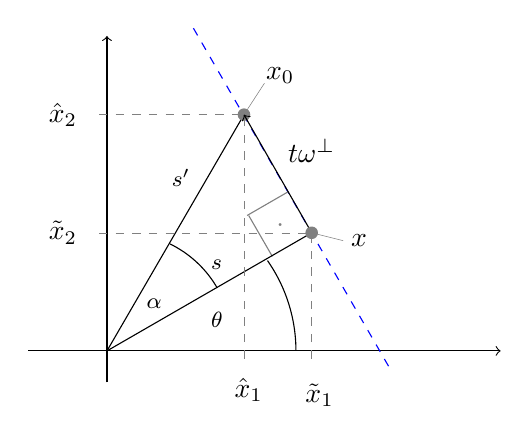
\begin{tikzpicture}[scale=2]		
			\draw [black] [->](-0.5,0) -- (2.5,0); % x-Achse
			\draw [black] [->](0,-0.2) -- (0,2); % y-Achse
			
			\draw [rotate=30, xshift=1.5cm, dashed] [blue] (0,1.5) -- (0,-1); % strahl
			
			\draw [xshift=1.05cm, yshift=0.6cm, rotate=120, - ] [gray] (0,0) -- (0.3,0);
			\draw [xshift=0.89cm, yshift=0.86cm, rotate=30, - ] [gray] (0,0) -- (0.3,0);
			\draw [gray] (1.1, 0.8)  node {$.$};
			
			\draw [black] [-] (0,0) -- (1.3,0.75); % s line
			\draw [black] (0.35, 1.1) node [right] {\footnotesize$s'$}; % s'
			\draw [dashed, very thin] [gray] (0.87,-0.05) -- (0.87,1.5); % \hat{x1} Projektion
			\draw [black] (0.9,-0.25)  node {$\hat{x}_1$};
			
			\draw [black] [-] (0,0) -- (0.87,1.5); % s' line
			\draw [black] (0.6, 0.55) node [right] {\footnotesize$s$}; % s
			\draw [dashed, very thin] [gray] (-0.05,1.5) -- (0.87,1.5); % \hat{x2} Projektion
			\draw [black] (-0.28,1.5)  node {$\hat{x}_2$};
			
			\fill[gray](0.87,1.5) circle [radius=0.04]; %x point 
			\draw[gray, very thin](0.87,1.5) -- (1, 1.7);
			\draw [black] (1.1, 1.75) node {$x_0$};
			
			\draw [black] [->] (1.3,0.75) -- (0.87,1.5); % t line
			\draw [black] (1.3,1.27) node {$t\omega^{\perp}$};	
			
			\fill[gray](1.3,0.75) circle [radius=0.04];
			\draw[gray, very thin](1.3,0.75) -- (1.5, 0.7);
			\draw [black] (1.6, 0.7) node {$x$};
			
			\draw [dashed, very thin] [gray] (1.3,-0.05) -- (1.3,0.75); % x-Projektion
			\draw [black] (1.35,-0.28)  node {$\tilde{x}_1$}; %\tilde{x1}
			
			\draw [dashed, very thin] [gray] (-0.05,0.75) -- (1.3,0.75); % y-Projektion		
			\draw [black] (-0.28,0.75)  node {$\tilde{x}_2$}; % \tilde{x2}
			
			\draw [black] (1.2,0) arc [start angle=0, end angle=35, radius=1cm]; % angle \theta
			\draw [black] (0.6, 0.2) node [right] {\footnotesize$\theta$};
			
			\draw [black] (0.7,0.4) arc [start angle=30, end angle=64, radius=0.7cm];
			\draw [black] (0.3, 0.3) node {\footnotesize$\alpha$};
		
		\end{tikzpicture}		
	\end{minipage}
	\begin{minipage}[b][5cm][t]{0.6\textwidth}
		\begin{align}
			& \beta = \alpha + \theta \label{equa:3.4}\\
			& x = \left(\begin{array}{c} \tilde{x_1} \\ \tilde{x_2} \end{array}\right) = s \left(\begin{array}{c} \cos(\theta) \\ \sin(\theta) \end{array}\right) = s\omega(\theta) \label{equa:3.5}\\
			& x_0 = \left(\begin{array}{c} \hat{x_1} \\ \hat{x_2} \end{array}\right) = s' \left(\begin{array}{c} \cos(\beta) \\ \sin(\beta) \end{array}\right) = s'\omega(\beta) \label{equa:3.6}\\
			& s'\omega(\beta) = s\omega(\theta) + t\omega^{\perp}(\theta)
			\label{equa:3.7}
		\end{align}
	\end{minipage}
	\caption{Eine Skizze (links) zur Verdeutlichung der Beziehung zweier Punkte $x_, x_0 \in \Omega$ bezüglich ihrer kartesischen- und Polar-Koordinaten. Die dazugehörige Nebenrechnung (rechts) zeigt deren formelmäßigen Zusammenhang auf.}
	\label{fig:3.4}
\end{figure}

Hier ist das Ziel zu zeigen dass, dass die ungefilterte Rückprojektion eine Faltung von $f(x) , \ x \in \Omega$ mit einer noch näher zu bestimmenden Funktion $h(x), \ x \in \Omega$ darstellt. Dazu formulieren wir folgendes Lemma:
\begin{lemma}
	Sei $f(x) \in L^2(\Omega)$ beliebig und $h(x) \in L^2(\Omega)$ speziell, dann kann die ungefilterte Rückprojektion als Faltung zweier Funktionen als
	\[ \mathcal{R^*} g(x_0) = \int \limits_{\R^2} f(x)h(x-x_0) \mbox{d}x = f(x)*h(x).\]	
	geschrieben werden. Da $\mbox{supp}f \subset \Omega$ betrachten wir das obige Integral nur auf $\Omega$.
	\label{lemma:3}
\end{lemma}
\begin{Bemerkung}
	Bevor wir zum Beweis übergehen, führen wir die dafür benötigte $\delta$-Distribution und einige für uns nützliche Eigenschaften ein. Seien $x, x_0 \in \R^2$, dann gilt:
	\begin{align}
	   	&  \ \  \delta(x-x_0) = \left\{ \begin{matrix} 0 & : &  x \neq x_0 \\ \infty & : & x = x_0 \end{matrix}\right. \label{equa:3.8}
   	\end{align}
	Eigenschaften :
	\begin{align}
		(\lowroman{1}).  &  \ \ \langle \delta(x-x_0), f(x)\rangle = \int \limits_{-\infty}^{\infty} f(x)\delta(x-x_0)\mbox{d}x = f(x_0) \label{equa:3.9}\\
		(\lowroman{2}). &  \ \  \delta(ax) = \frac{1}{|a|}\delta(x) \label{equa:3.10} \\
		(\lowroman{3}). &  \ \  \int \limits_{-\infty}^{-\infty}\delta(x-x_0) \mbox{d}x = 1 \label{equa:3.11}
	\end{align}
	\label{bem:8}
\end{Bemerkung}
\begin{proof}
	Wir Beginen mit der Definition der ungefilterten Rückprojektion (\ref{equa:1.21}) und benutzen dabei die Nebenrechnung zu Abb. \ref{fig:3.4} sowie die eingeführten Eigenschaften der $\delta$-Distribution aus der Bemerkung \ref{bem:8}.
	\begin{equation}
	\begin{split}
		\mathcal{R^*} g(x_0) & = \int\limits_{0}^{\pi} \ g(x_{0}^{T}\omega(\theta),\theta) \ \mbox{d}\theta  \ \  \stackrel{(\ref{equa:1.10}, \ \ref{equa:3.7})}{=} \ \ \int\limits_{0}^{\pi} \left( \int\limits_{-\gamma(s)}^{\gamma(s)} f(s'\omega(\beta)) \ \mbox{d}t \right) \mbox{d}\theta \\
		& \stackrel{(\ref{equa:3.9})}{=} \int\limits_{0}^{\pi} \left( \int\limits_{-\gamma(s)}^{\gamma(s)} \int\limits_{-1}^{1} f(s\omega(\theta)) \delta(s\omega(\theta) - s'\omega(\beta)) \ \mbox{d}s \ \mbox{d}t \right) \mbox{d}\theta \\
		& \stackrel{(\ref{equa:3.7})}{=} \int\limits_{0}^{\pi} \left( \int\limits_{\Omega} f(x) \delta(t\omega^{\perp}(\theta)) \ \mbox{d}x \right) \mbox{d}\theta \stackrel{(\ref{equa:3.10})}{=} \int\limits_{\Omega} f(x) \frac{\int\limits_{0}^{\pi}\delta(\beta - \alpha)\mbox{d}\beta}{|t\frac{\partial \omega^{\perp}(\theta)}{\partial \theta}|} \mbox{d}x \\
		& \stackrel{(\ref{equa:3.11})}{=} \int\limits_{\Omega} f(x) \frac{1}{|x - x_0|} \mbox{d}x = f(x)*h(x).
	\end{split}
	\label{equa:3.12}
	\end{equation}
	In der letzten Zeile wurde $|t\frac{\partial \omega^{\perp}(\theta)}{\partial \theta}| = |t||\left(\begin{array}{c} -\cos(\theta) \\ -\sin(\theta) \end{array}\right)| = |t| = |x -x_0|$ benutzt.
\end{proof}
Somit haben wir auch die spezielle Funktion $h(x) = \frac{1}{|x|}$ gefunden. Die Funktion $h$ heißt \textit{Point-Spread-Function}. Anschaulich kann $f$ in jedem Punkt als $\delta$-Distribution verstanden werden. Das heißt, setzt man $f$ auf ganz $\Omega$ Null, außer im Punkt $x_0 \in \Omega$ und faltet mit $h(x)$, so wird das Ergebnis $\tilde{f}$ um den Punkt $x_0$ nach außen radial abfallen. Führt man die Faltung von $f$ für jeden Punkt in $\Omega$ und setzt auf diese Weise entstandene Faltungsbilder zusammen führt das zu dem Effekt der Verschwommenheit. 

\subsection{Gefilterte Rückprojektion}
\label{cha:3.1.2}

Das in dem letzten Abschnitt erreichte Ergebnis ist für die Praxis unbrauchbar. Man kann an einem verschwommenen Bild keine qualitative Analyse durchführen. Deshalb werden wir in diesem Abschnitt eine Verbesserung des ersten Verfahrens suchen. Wie der Name schon verrät, bekommt man ein ungefiltertes Bild zurück. Wir wollen nun verstehen, wie man die Projektionsdaten filtert, bevor man sie zurück projiziert.

Um den Ausdruck der \textit{gefilterten Rückprojektion} zu bekommen, werden wir uns des sogenannten \textit{Fourier\footnote{Jean Baptiste Joseph Fourier (1768 - 1830) ein französischer Mathematiker und Physiker.}-Slice-Theorem} (FST) bedienen (siehe z.B. \cite[S. 120]{Buzug04}). Das Schema des Theorems kann nun folgendermaßen wiedergegeben werden:
\begin{enumerate}
	\item Berechne für einen festen Winkel $\theta$ die Fouriertransformierte\footnote{
		\label{foot:14}\textbf{Definition }\textit{Fourier-Transformation}. Sei $f(x) \in L^2(\Omega)$, dann ist ihre Fourier-Transformation durch
			\begin{equation}
				(\mathcal{F}f)(x) = \int \limits_{\Omega} f(x) e^{-2\pi i \langle x^T, u \rangle} \mbox{d}x = F(u), \ \ u \in \mathbb{C}^2
				\label{equa:3.13}
			\end{equation}
		gegeben.} (FT) einer Projektion $\mathcal{R}f(s,\theta) = g(s,\theta)$
	\[(\mathcal{F}g)(s,\theta) = G(q, \theta). \]
	\item Konstruiere die Fouriertransformierte $F(u,v)$ von $f(x)$ aus $G(q,\theta)$
	\[G(q,\theta) \leadsto F(u).\]
	\item Berechne die inverse Fouriertransformierte von $F$
	\[(\mathcal{F}^{-1}F)(u) = \tilde{f}(x). \]
\end{enumerate}

Wir werden den Punkt 2 des FST vom Punkt 1 und dann vom Punkt 3 aus schrittweise annähern. Bevor wir die Herleitung der gefilterten Rückprojektion angehen, machen wir uns die vorliegende Situation an einer Skizze (Abb. \ref{fig:3.5}) klar. 

In der Abbildung \ref{fig:3.5} ist schematisch wiedergegeben, dass die Fourier-Transformation an der Natur der Koordinatensysteme nichts ändert. Diese Tatsache wird in dem \textit{Plancherel-Theorem} bewiesen, welches unter anderem besagt, dass die die FT ein \text{unitärer} Operator für Funktionen aus $L^2$ ist. Das heißt, die FT ist linear, isometrisch und bijektiv. Das weiteren beweist der Satz die Invertierbarkeit von $\mathcal{F}$ für $L^2$ Funktionen. 
\begin{figure}[!h]
	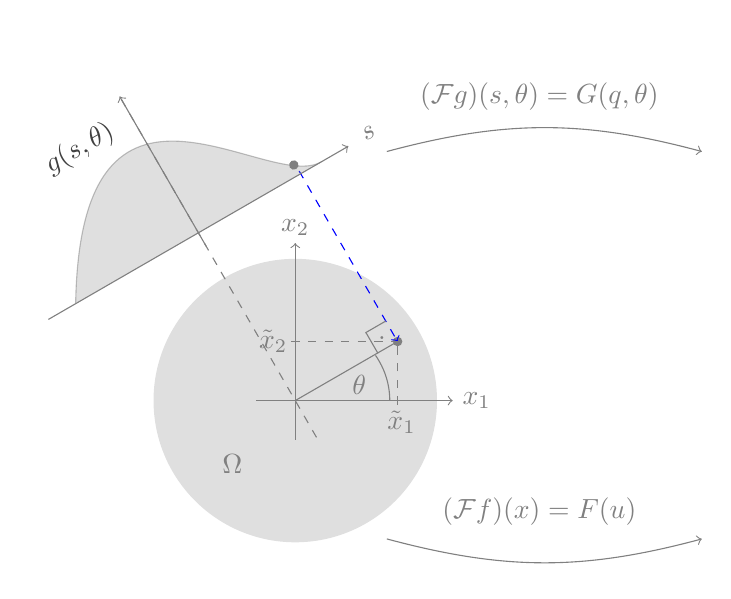
\begin{tikzpicture}[xshift=-100]%, scale=0.75]
		\fill[nearly transparent, color=gray] (0,0) circle (1.8cm);
		\draw [gray] [->](-0.5,0) -- (2,0); % x-Achse
		\draw [gray] (2, 0) node [right] {$x_1$};
		
		\draw [gray] [->](0,-0.5) -- (0,2); % y-Achse
		\draw [gray] (0, 2.2) node {$x_2$};
	
		\fill[gray](1.3,0.75) circle [radius=0.06]; % ein Punkt		
	
		\draw [rotate=30, xshift=1.5cm, ->, dashed] [blue] (0,2.5) -- (0,0); % strahl		
		
		\draw [xshift=1.05cm, yshift=0.6cm, rotate=120, - ] [gray] (0,0) -- (0.3,0);
		\draw [xshift=0.89cm, yshift=0.86cm, rotate=30, - ] [gray] (0,0) -- (0.3,0);
		\draw [gray] (1.1, 0.8)  node {$.$};
		
		\draw [rotate=30] [gray] [-] (0,0) -- (1.5, 0);
		
		\draw [dashed] [gray] (1.3,-0.05) -- (1.3,0.75); % x-Projektion
		\draw [gray] (1.35,-0.28)  node {$\tilde{x}_1$};
		
		\draw [dashed] [gray] (-0.05,0.75) -- (1.3,0.75); % y-Projektion		
		\draw [gray] (-0.28,0.75)  node {$\tilde{x}_2$};
		
		\draw [lightgray] [rotate=30, yshift=70] (-1.8,0) .. controls (0,3) and (1,0) .. (1.8,0);
		\fill [nearly transparent, color=gray] [rotate=30, yshift=70] (-1.8,0) .. controls (0,3) and (1,0) .. (1.8,0);
		
		\fill[ rotate=30, xshift=0.18cm, yshift=1.85cm, gray](1.3,0.75) circle [radius=0.06]; % ein Punkt
		
		\draw [rotate=30, xshift=0, yshift=70] [gray] [->] (-2.2,0) -- (2.2, 0); % s line
		\draw [gray] (3.7, 0)  node [rotate=30, xshift=-20, yshift=123] {$s$};
		
		\draw [rotate=120, xshift=70 ] [gray] [->] (-0.2,0) -- (2, 0);	% g(s, \theta) line	
		\draw [rotate=120, xshift=70 ] [gray, dashed] [-] (-3,0) -- (2, 0);		
		\draw [darkgray] (-0.2, 0)  node [left, rotate=30, yshift=115] {$g(s, \theta)$};		
		
		\draw [gray] (1.2,0) arc [start angle=0, end angle=35, radius=1cm];
		\draw [gray] (0.6, 0.2) node [right] {$\theta$};
		
		\draw [gray] (-0.8, -0.8) node {$\Omega$};
		
		\draw [gray] (3.1, 0) [rotate=0, xshift=0, yshift=110] node {$(\mathcal{F}g)(s,\theta) = G(q, \theta)$};
		\draw[->, gray] [rotate=0, xshift=90, yshift=90] (-2,0) to[out=15, in=165] (2,0);
		
		\draw [gray] (3.1, 0) [rotate=0, xshift=0, yshift=-40] node {$(\mathcal{F}f)(x) = F(u)$};
		\draw[->, gray] [rotate=0, xshift=90, yshift=-50] (-2,0) to[out=-15, in=195] (2,0);	
	\end{tikzpicture}
	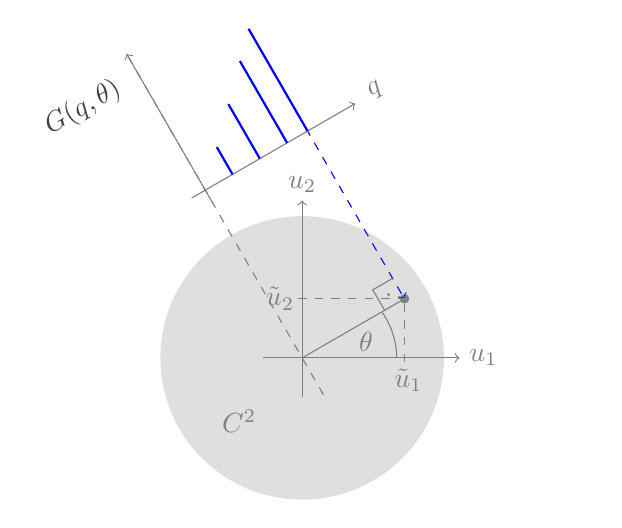
\begin{tikzpicture}[xshift=50]	
		\fill[nearly transparent, color=gray] (0,0) circle (1.8cm);
		\draw [gray] [->](-0.5,0) -- (2,0); % x-Achse
		\draw [gray] (2, 0) node [right] {$u_1$};
		
		\draw [gray] [->](0,-0.5) -- (0,2); % y-Achse
		\draw [gray] (0, 2.2) node {$u_2$};
		
		\fill[gray](1.3,0.75) circle [radius=0.06]; % ein Punkt		
		
		\draw [rotate=30, xshift=1.5cm, ->, dashed] [blue] (0,2.5) -- (0,0); % strahl		
		
		\draw [xshift=1.05cm, yshift=0.6cm, rotate=120, - ] [gray] (0,0) -- (0.3,0);
		\draw [xshift=0.89cm, yshift=0.86cm, rotate=30, - ] [gray] (0,0) -- (0.3,0);
		\draw [gray] (1.1, 0.8)  node {$.$};
		
		\draw [rotate=30] [gray] [-] (0,0) -- (1.5, 0);
		
		\draw [dashed] [gray] (1.3,-0.05) -- (1.3,0.75); % x-Projektion
		\draw [gray] (1.35,-0.28)  node {$\tilde{u}_1$};
		
		\draw [dashed] [gray] (-0.05,0.75) -- (1.3,0.75); % y-Projektion		
		\draw [gray] (-0.28,0.75)  node {$\tilde{u}_2$};
	
		\draw [rotate=30, xshift=0, yshift=70] [gray] [->] (-0.2,0) -- (2.2, 0);
		\draw [gray] (3.7, 0)  node [rotate=30, xshift=-20, yshift=123] {$q$};
		
		\draw [rotate=120, xshift=70 ] [gray] [->] (-0.2,0) -- (2, 0);	% g(s, \theta) line	
		\draw [rotate=120, xshift=70 ] [gray, dashed] [-] (-3,0) -- (2, 0);		
		\draw [darkgray] (-0.2, 0)  node [left, rotate=30, yshift=115] {$G(q, \theta)$};			
		
		\draw [gray] (1.2,0) arc [start angle=0, end angle=35, radius=1cm];
		\draw [gray] (0.6, 0.2) node [right] {$\theta$};
		
		\draw [gray] (-0.8, -0.8) node {$\mathbb{C}^2$};
		
		\foreach \x in {0, 0.4, 0.8, 1.2, 1.5}
		{
			\draw[rotate=30, xshift=0, yshift=70][blue, thick] (\x,\x) -- (\x,0); 
		}
	\end{tikzpicture}
	\caption{Eine Veranschaulichung des Fourier-Slice-Theorems. Links ist der Vorgang der Radon Transformation abgebildet, rechts seine Fouriertransformierte.}
	\label{fig:3.5}
\end{figure}

Jetzt haben wir genug Argumente gesammelt, um die gefilterte Rückprojektion herzuleiten. Dafür beginnen wir mit dem Punkt 1 des FST: wir bilden die Fouriertransformierte (Fußnote \ref{foot:14}) einer Projektion $p(s, \theta)$:
\begin{equation}
	\begin{split}
		P(q, \theta) & = \int \limits_{-1}^{1} p(s, \theta) e^{-2\pi i qs} \mbox{d}s \\
		&  \stackrel{(\ref{equa:1.10})}{=} \int \limits_{-1}^{1} \left( \int\limits_{-\gamma(s)}^{\gamma(s)} f(s\omega(\theta) + t\omega^{\perp}(\theta)) \mbox{d}t \right) e^{-2\pi i qs} \mbox{d}s \\
		& \stackrel{(\ref{equa:1.22})}{=} \int \limits_{\Omega} f(x) e^{-2\pi i q x^T\omega(\theta)}\mbox{d}x.	
	\end{split}
	\label{equa:3.14}
\end{equation}	
An dem Punkt 3 des FST ist nicht viel zu tun, deshalb geben wir hier direkt die Fouriertransformierte von $f$ an. Bei der Wahl der Koordinaten für $\mathcal{F}f$ und ihre Umrechnung stützen wir uns auf die rechte Seite der Abbildung \ref{fig:3.5}. Dann gilt 
\begin{equation}
	 F(q\cos(\theta), q\sin(\theta)) = \int \limits_{\Omega}^{} f(x)e^{-2\pi i qx^T\omega(\theta)} \mbox{d}x.
	\label{equa:3.15}
\end{equation}
Aus den Gleichungen (\ref{equa:3.14}) und (\ref{equa:3.15}) können wir festhalten, dass die Fouriertransformierten von $f$ und $p$ im folgenden Bezug zueinander stehen
\begin{equation}
	F(q\cos(\theta), q\sin(\theta)) =  P(q, \theta).
	\label{equa:3.16}
\end{equation}   
Das heißt (\ref{equa:3.16}) soll eine Koordinatentransformation zwischen $\mathcal{F}f$ und $\mathcal{F}p$ darstellen. Somit ist der Punkt 2 des FST auch erledigt.

Im zweiten Schritt invertieren wir die Gleichung (\ref{equa:3.15}) und führen eine Variablensubstitution\footnote{Für die Substitution von $\mbox{d}u_1\mbox{d}u_2$ berechnen wir die Jacobi-Determinante von $ |J(\left(\begin{array}{c} u_1 \\ u_2 \end{array}\right)) = \left| \left(\begin{pmatrix}{c} \cos(\theta) & \sin(\theta) \\ -q\sin(\theta) & q\cos(\theta) \end{pmatrix}\right)\right| = q$, somit erhalten wir $\mbox{d}u_1\mbox{d}u_2 = q\mbox{d}q\mbox{d}\theta$.} durch, sodass man zu der Gleichung  
\begin{equation}
	f(x) = \int \limits_{0}^{\pi} \int \limits_{-1}^{1}F(q\cos(\theta), q\sin(\theta))e^{2\pi i qx^T\omega(\theta)} q \ \mbox{d}q \ \mbox{d}\theta
	\label{equa:3.17}
\end{equation}
gelangt. Die Symmetriebetrachtungen, wie in \cite[S. 135]{Buzug04} und die Tatsache, dass man nur reelle Funktionen auf $\Omega$ betrachtet, führen zu folgendem Ausdruck
\begin{equation}
	\begin{split}
		f(x) & = \int \limits_{0}^{\pi} \int \limits_{-1}^{1}F(q\cos(\theta), q\sin(\theta))e^{2\pi i qx^T\omega(\theta)} |q| \ \mbox{d}q \ \mbox{d}\theta \\
		& \stackrel{(\ref{equa:3.16})}{=} \int \limits_{0}^{\pi} \left( \int \limits_{-1}^{1} \left( \ P(q, \theta)|q| \ \right) e^{2\pi i qx^T\omega(\theta)} \ \mbox{d}q \right) \mbox{d}\theta.
	\end{split}
	\label{equa:3.18}
\end{equation}

Mit der Gleichung (\ref{equa:3.18}) haben wir die gefilterte Rückprojektion erhalten. Es bleibt noch das Gefilterte darin zu entdecken. Beginnen wir mit der inneren Klammerung von (\ref{equa:3.18}). $P(q, \theta)$ ist die Fouriertransformierte $\mathcal{F}p$ von $p(s,\theta)$, die punktweise mit einer Betragsfunktion $b(q) = |q|$ multipliziert wird. Da wir jetzt $p(s, \theta)$ im Frequenzraum betrachten und die Funktion $b(q)$ über das gleiche Frequenzband, wie $P(q,\theta)$ läuft, werden durch punktweise Multiplikation kleinfrequente Anteile von $P(q,\theta)$ von $b(q)$ unterdrückt und die hochfrequente im Gegensatz sehr verstärkt. Dieses Vorgehen wird im Allgemeinen \textit{Hochpassfilterung} genannt. Die Funktion $b(q) = |q|$ bezeichnet man als Rampenfilter. Im Folgenden bezeichnen wir einen Filter mit $h_{\xi}(q)$ und wir schreiben $h_{b}(q) = b(q) = |q|$. Für die Filterung der Projektionen führen wir die Bezeichnung $P_{h_{\xi}}(q, \theta) = P(q, \theta)h_{\xi}(q)$ ein.

Nach dem die Filterung der Projektion durchgeführt wurde, wird diese mittels der inversen FT zurück in den Ortsrum der Projektionen überführt. Was durch das innere Integral von (\ref{equa:3.18}) dargestellt wird. Anschließend projiziert man die gefilterte Projektion in den Ortsraum von $f$ zurück, dies ist das äußere Integral von (\ref{equa:3.18}). 

Wir fassen die nötigen Schritte der gefilterten Rückprojektion zu einem Algorithmus zusammen
\begin{algorithm}
	\caption{Gefilterte Rückprojektion (Filtered Back Projection, FBP)}
	\begin{algorithmic}[1]	
		\State Berechne die FT von $(\mathcal{F}p)(s, \theta) = P(s, \theta)$.
		\State Führe die Fiterung $P_{h_{\xi}}(q, \theta) = P(q, \theta)h_{\xi}(q)$ durch.
		\State Berechne die inverse FT $(\mathcal{F}^{-1}P_{h_{\xi}})(q, \theta) = \tilde{p}(s,\theta)$.
		\State Projiziere $\tilde{p}(s,\theta)$ auf $\Omega$ zurück. 
	\end{algorithmic}
	\label{alg:3.1}
\end{algorithm}

In der Abbildung \ref{fig:3.6.b} ist das erste Ergebnis der gefilterten Rückprojektion, gefiltert mit einem Rampenfilter zu sehen. 

Wenn man das Sinogramm (Abb. \ref{fig:3.2.b}) betrachtet, so stellt man fest, dass das Sinogramm keine Störungen aufweist. Das würde eine perfekte Messung bedeuten. Dies ist aber bei den realen Messungen nie der Fall. Deshalb wollen wir uns die Rekonstruktion von gestörten Daten anschauen. Dafür soll das Phantom Bild (Abb. \ref{fig:3.2.a}) mit einem Salzstreuer-Effekt (Quelle: \MATLAB) beaufschlagt werden. Das soll die Homogenität einiger Pixelbereiche von der Abbildung \ref{fig:3.2.a} aufheben, was eine kleine Annäherung zur Realität widerspiegelt (Abb. \ref{fig:3.7.a}).  
\begin{figure}[!h]
	\begin{center}
		\subfloat[\label{fig:3.6.a}Das Rampenfilter.]{{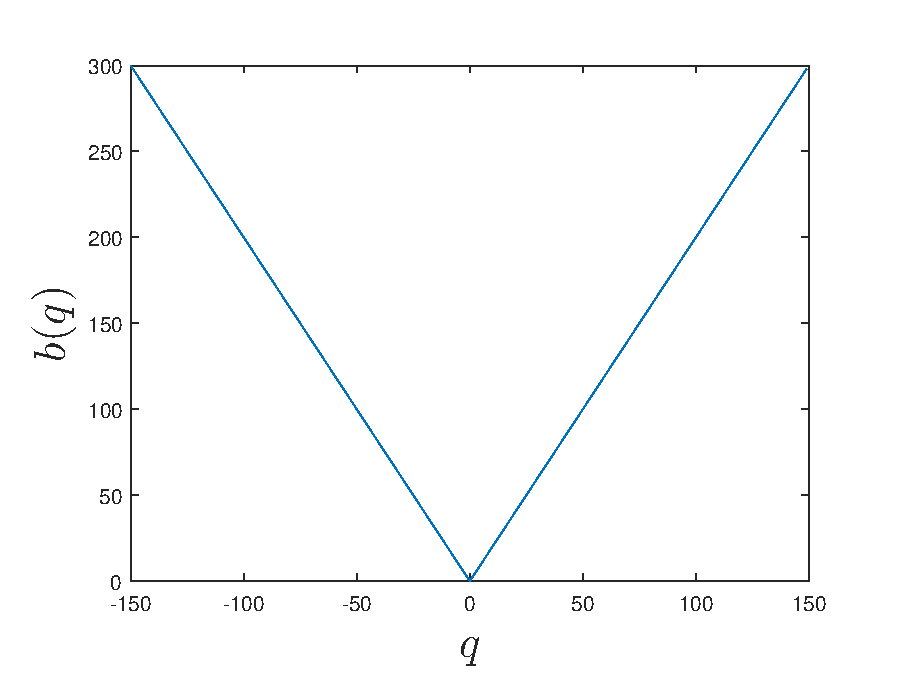
\includegraphics[width=0.5\textwidth]{rampFilter.eps} }}
		\subfloat[\label{fig:3.6.b}Eine mit Rampenfilter gefilterte Rückprojektion.]{{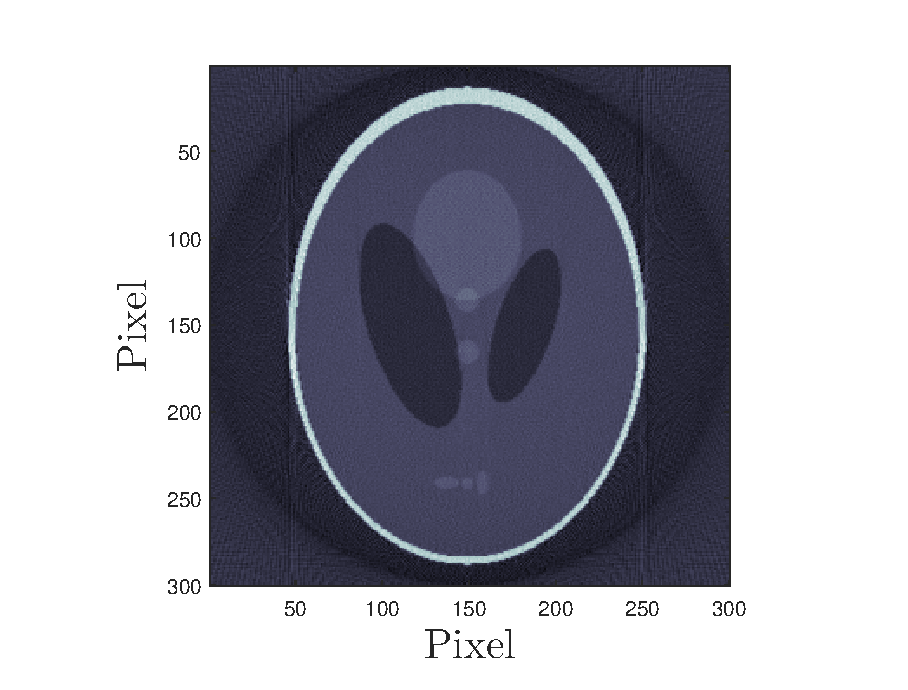
\includegraphics[width=0.5\textwidth]{rampFiltered.eps} }}
	\end{center}
	\caption{ Links (a) das Rampenfilter, konstruiert passend zu dem Sinogramm aus \ref{fig:3.2.b}. Das Frequenzband des Filters ist durch die isometrische Eigenschaften der FT gleich der Detektorbreite, also ist auch gleich der Tiefe des Sinogramms. Rechts (b) ist die gefilterte Rückprojektion von \ref{fig:3.2.b}, durchgeführt unter der Einwirkung des Rampenfilters aus (a).}
	\label{fig:3.6}
\end{figure} 

Die Radon Transformation von der Abbildung \ref{fig:3.7.a} ohne zusätzliche Störung würde nicht die Messfehler repräsentieren, höchstens Rundungsfehler, die bei der Integration entstehen, hier aber nicht wesentlich sind. Deshalb stören wir die Projektionsdaten zusätzlich mit dem Salzstreuer-Effekt (Abb. \ref{fig:3.7.b}).
\begin{figure}[!h]
	\begin{center}
		\subfloat[\label{fig:3.7.a}Ein verrauschtes Phantombild.]{{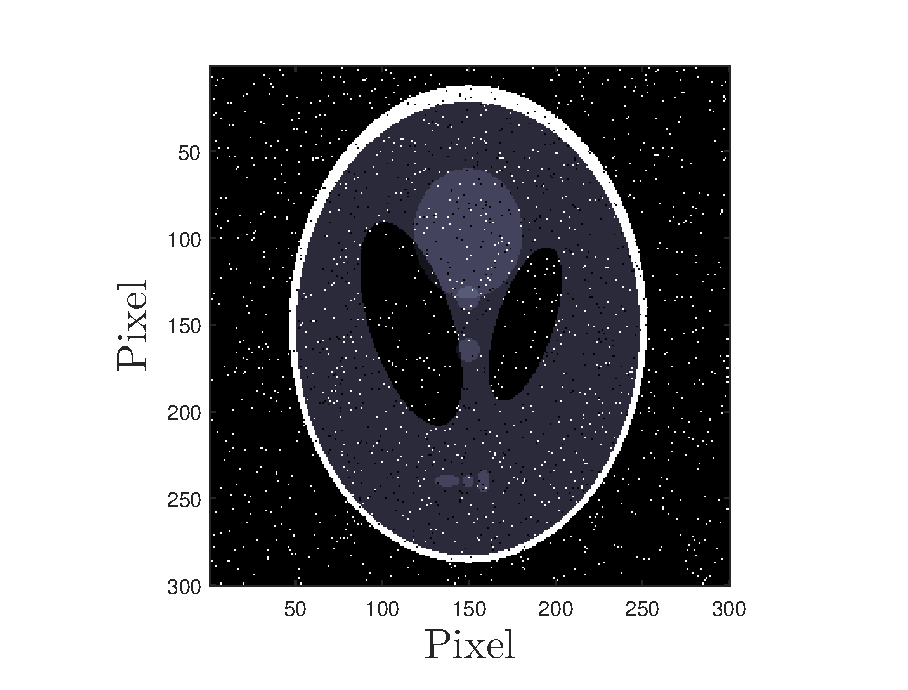
\includegraphics[width=0.5\textwidth]{noisedPhantom.eps} }}
		\subfloat[\label{fig:3.7.b}Die Radontransformierte von (a) und einem zusätzlichem Rauschen.]{{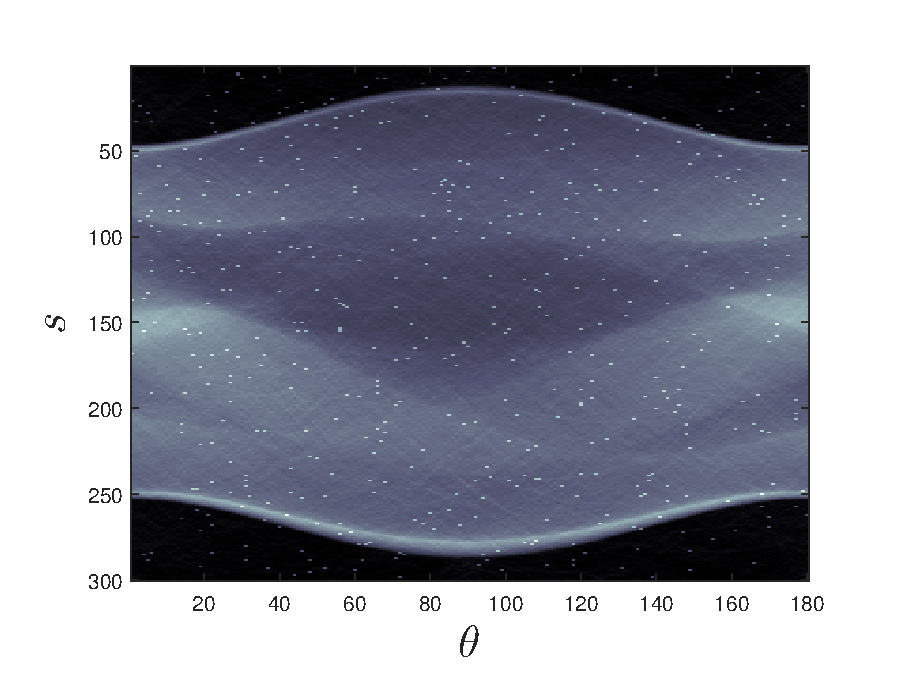
\includegraphics[width=0.5\textwidth]{rt_noised.eps} }}
	\end{center}
	\caption{ Links (a) ist ein Phantombild verrauscht mit einem Salzstreuer-Effekt (Quelle: \MATLAB) dargestellt. Rechts (b) ist Die Radontransformierte von (a) und zusätzlich mit einem Salzstreuer-Effekt verrauscht.}
	\label{fig:3.7}
\end{figure} 

Wir erinnern uns an die Ergebnisse des zweiten Kapitels. Insbesondere daran, dass der Operator $\mathcal{R}$ schlecht gestellt ist. Dazu sei die Gleichung (\ref{equa:2.3}) nochmal betrachtet
\[\mathcal{R}^{+} g  = \sum\limits_{j = 1}^{n} \sigma_j^{-1} \langle g, u_j \rangle_{L^2(Z)} v_j.\]
Wir wissen, dass $g$ die Projektionen in (\ref{equa:2.3}) darstellt. Sei nun $p_{\epsilon}$ unsere gestörte Projektion. Des Weiteren betrachten wir den Schritt 2,3 des Algorithmus \ref{alg:3.1} und schreiben ihn, wie folgt auf
\begin{eqnarray}
	\tilde{p}_{\epsilon} = \int \limits_{-1}^{1} P(q, \theta)h_{\xi}(q) e^{2\pi i qx^T\omega(\theta)} \ \mbox{d}q.
	\label{equa:3.19}
\end{eqnarray}
Wir wollen nun $\tilde{p}_{\epsilon}$ als eine Linearkombination oder auch als verallgemeinerte Fourierreihe angeben. Das tun wir direkt für den diskreten Fall unter Beachtung der Bemerkung \ref{bem:5}. Somit bekommen wir
\begin{equation}
	\tilde{p}_{\epsilon} \approx \sum \limits_{i = 1}^{n} c_ih_{\xi}(q_i)u_i, \ \ \mbox{mit} \  c_i = \langle \tilde{P}, u_i \rangle.
	\label{equa:3.20}
\end{equation} 
Diese Gleichung werden wir nicht beweisen, aber praktisch bedeutet das, wenn man $h_{\xi}(q) = 1$ setzt und es dem FBP Algorithmus übergibt, kommt genau die ungefilterte Projektion dabei raus.
\begin{figure}[!h]
	\centering
	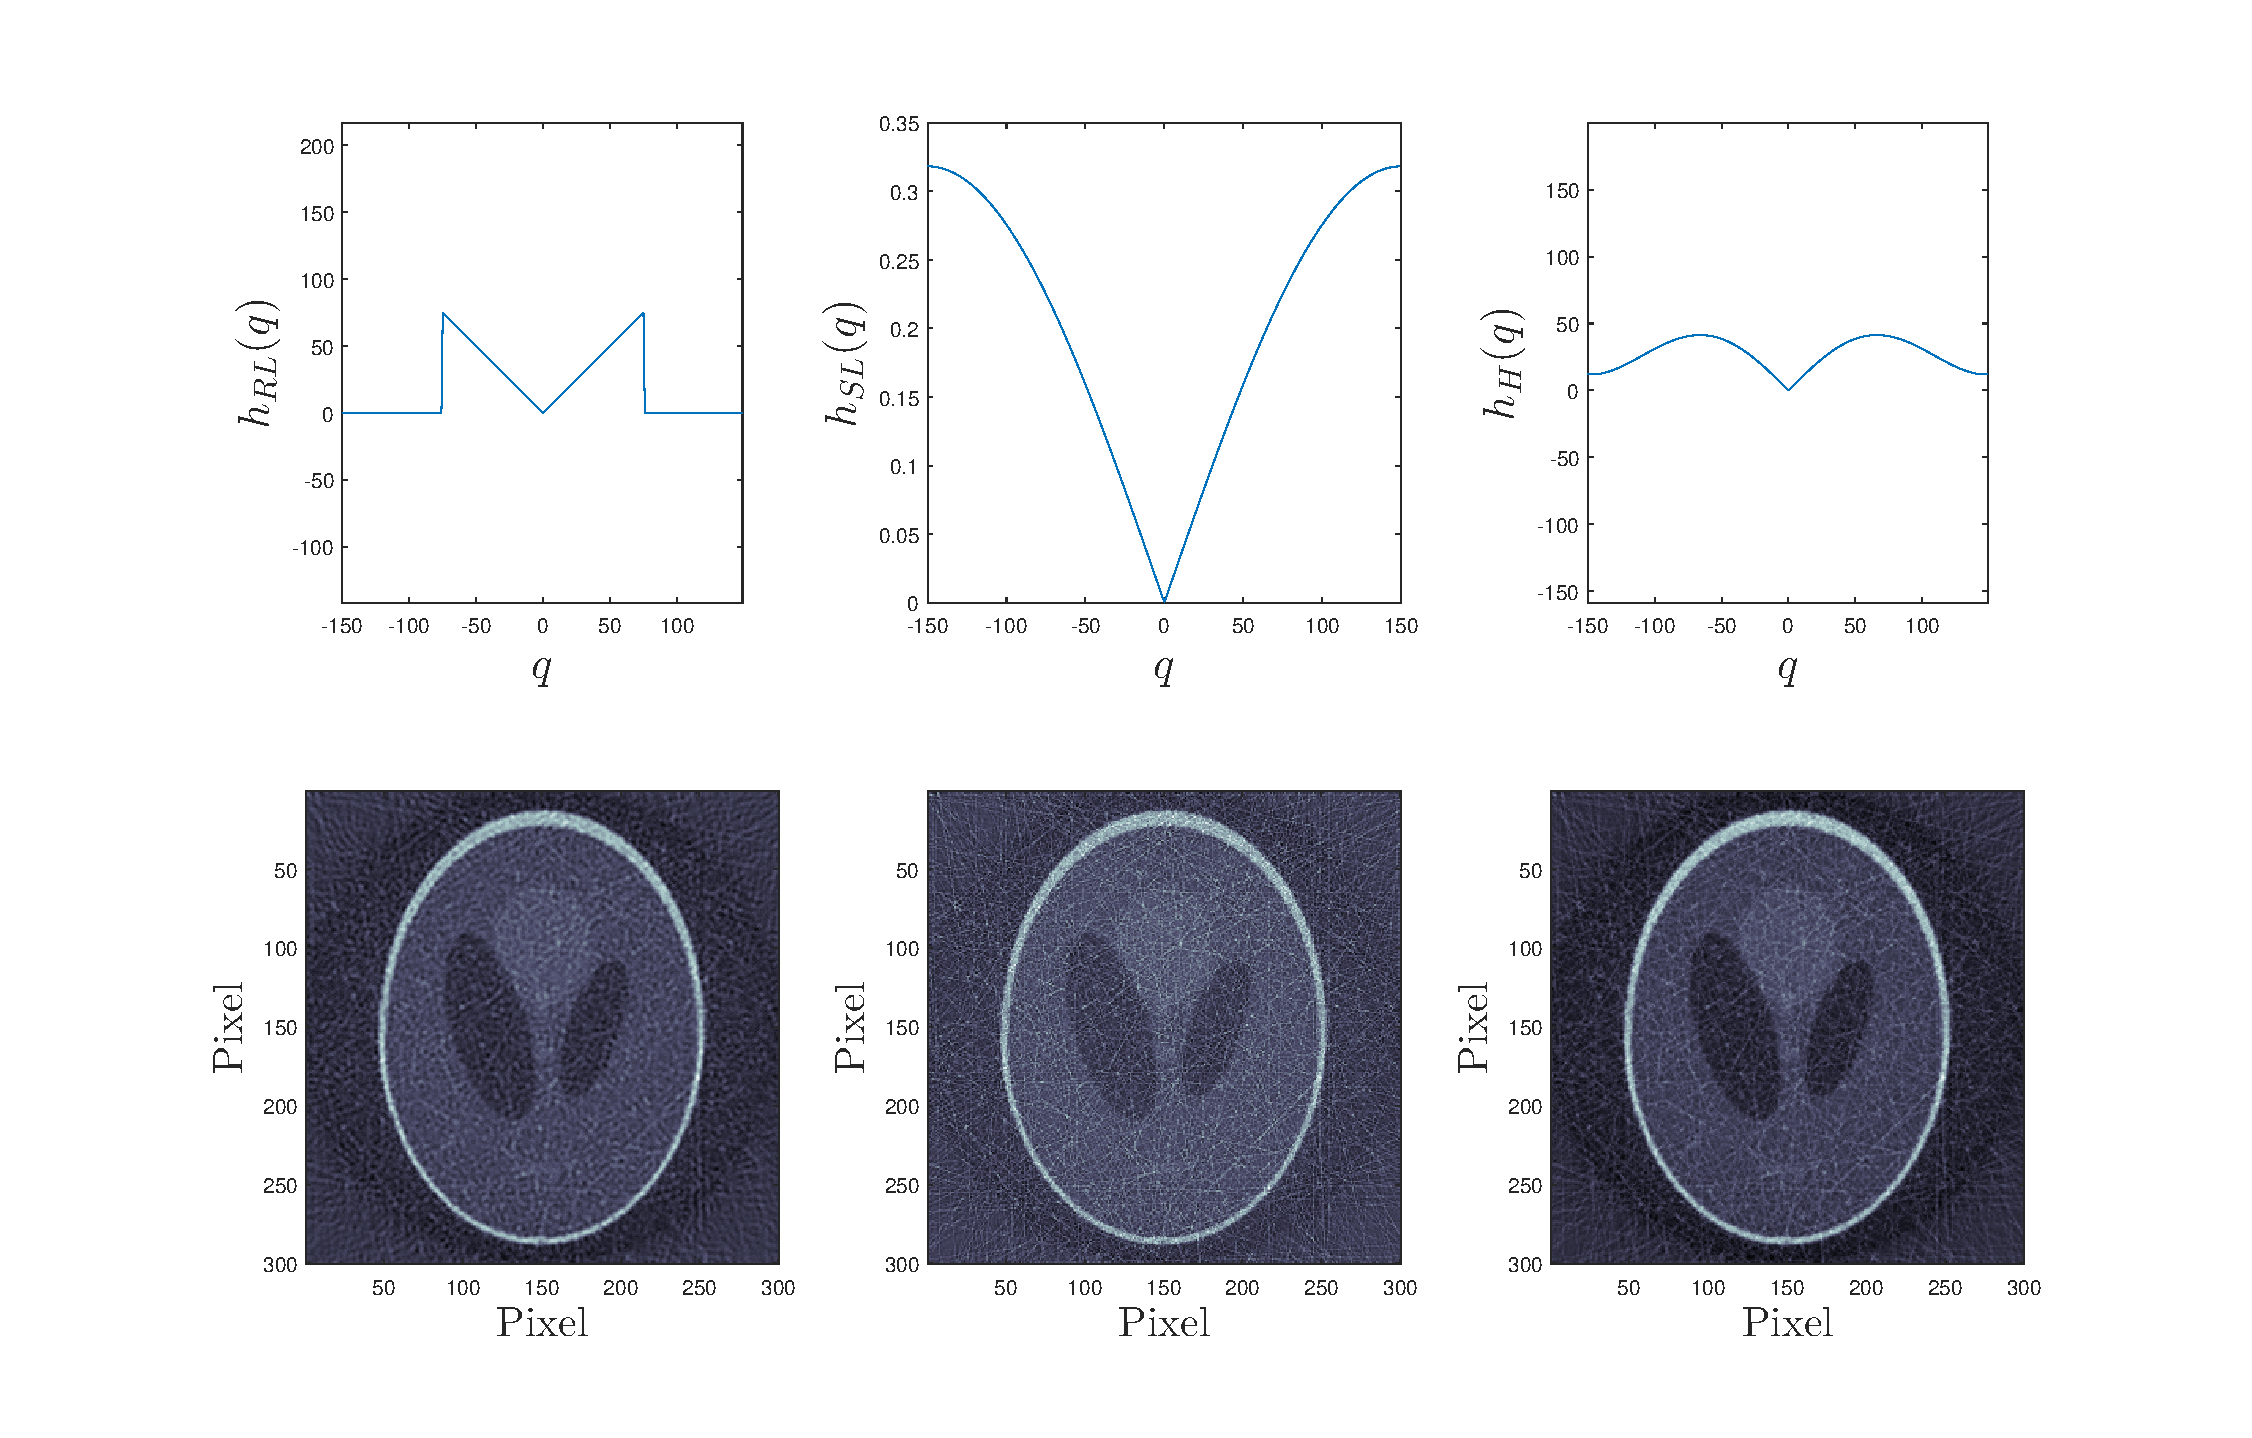
\includegraphics[width=1\textwidth]{diffFilter.eps}
	\caption{Eine Rekonstruktion aus den Daten \ref{fig:3.7.b} unter der Einwirkung von drei verschiedenen Filtern. Unten links ist die Filterung mit dem \textit{Ramachandran-Lakshminarayanan-Filter}, mittig mit dem \textit{Shepp-Logan-Filter} und rechts mit dem \textit{Hamming-Fiter} dargestellt.}  
	\label{fig:3.8}
\end{figure}

Nun setzen wir unsere gestört-gefilterte Projektion (\ref{equa:3.20}) in (\ref{equa:2.3}) ein und bekommen einen Ausdruck
\begin{equation}
	\begin{split}
		\mathcal{R}^{+} g & = \sum\limits_{j = 1}^{n} \sigma_j^{-1} \langle \left( \sum \limits_{i = 1}^{n} c_i h_{\xi}(q_i) u_i \right), u_j \rangle_{L^2(Z)} v_j \\
		& = \sum\limits_{j,i = 1}^{n} ( \sigma_j^{-1} h_{\xi}(q_j) ) c_i \delta_{ij} v_j = \sum\limits_{j = 1}^{n} ( \sigma_j^{-1} h_{\xi}(q_j) ) c_i v_j,
	\end{split}
	\label{equa:3.21}
\end{equation}
der uns prinzipiell keine neue Erkenntnis liefert, aber offensichtlich macht, wie die hochfrequenten Anteile bei der Rekonstruktion von dem Filter beeinflusst werden können. Das heißt, das Design des Filters kann die Rückprojektion in verschiedenen Frequenzbereichen dämpfen und somit ihre Oszillation bis zu einem gewissen Grade beschränken. Anders gesagt, wir beschleunigen somit die Konvergenz der Reihe (\ref{equa:3.21}) zu unseren Gunsten. 

In der Abbildung \ref{fig:3.8} sind drei Ergebnisse mit drei verschiedenen Filtern dargestellt. Zum Aufbau verschiedener Filterkerne sei man hier auf \cite[S. 191]{Buzug04} verwiesen. In der Abbildung \ref{fig:3.8} links unten, ist zu erkennen, dass ein \textit{Ramachandran-Lakshminarayanan-Filter} die hohen Frequenzen abschneidet, wodurch das Bild insgesamt an Kontrast verliert. Das untere Ergebnis in der Mitte zeigt, dass das \textit{Shepp-Logan-Filter} die mittleren Frequenzen anhebt, was die Helligkeit des Ergebnisses etwas erhöht. Das untere rechte Bild hat durch das \textit{Hamming-Fiter} volles Frequenzband erhalten, allerdings sind die hohen Frequenzen stark gedämpft worden.

Insgesamt existiert ein Dutzend Filter, die bei der CT-Bildrekonstruktion eingesetzt werden können. Dieses Vorgehen nennt man \textit{Regularisierung} des Rückprojektionsproblems mit Filtern.  

\section{Algebraische Rekonstruktionsverfahren}
\label{cha:3.2}

Algebraische Verfahren basieren auf der Auffassung des Operators $\mathcal{R}$ als eine Matrix. Das hat zu Folge, dass man die Wirkung von $\mathcal{R}$ auf $f$ in Form eines linearen Gleichungssystems auffassen kann. Somit bekommen wir
\begin{equation}
	\mathcal{R}f = Af = p.
	\label{equa:3.22}
\end{equation}
\begin{Bemerkung}
	Für den Rest dieses Kapitels vereinbaren wir nur diskretisierte Systeme zu betrachten. 
	\label{bem:9}
\end{Bemerkung}
Mit der Bemerkung \ref{bem:9} und den vereinbarten Größen $f \in \R^m$ (\ref{equa:3.2}) und $p \in \R^n$ (\ref{equa:3.1}) ist $A$ eine endliche Matrix. $A$ wird \textit{Systemmatrix} des Abbildungssystems von $\mathcal{R}$ genannt. Wir werden zunächst die Entstehung und den Aufbau von $A$ etwas genauer anschauen. 

\subsubsection{Aufbau der Systemmatrix $A$ von $\mathcal{R}$}

Da $f \in \R^m$ und $p \in \R^n$ sind bedeutet es, dass $A \in \R^{n\times m}$ ist. Das heißt, die Zeilen von $A$ laufen über die Indizierung der Projektionen $p$, also die Zeile $j$ ist die $j$-te Projektion. Die Spalten von $A$ laufen über die Indizierung von $f$.

$f$ wird durch die Anzahl der Detektoren $k$ im Detektorband diskretisiert (Abb. \ref{fig:3.9}). Man kann also hypothetisch $f \in \R^{k\times k}$ annehmen. Lassen wir die Indizierung von $f$ Zeilenweise durchlaufen, so kommen wir genau auf $f \in \R^{k^2}$. Wobei nach (\ref{equa:3.2}) $k^2= m$ gilt.

Aus der Gleichung (\ref{equa:3.22}) können wir folgern, dass für $j$-te Projektion
\begin{equation}
	\sum \limits_{i = 1}^{m} a_{ji}f_i = p_j
	\label{equa:3:23}
\end{equation}
gelten muss. Beachtet man, dass nur die $f_j$ die vom Strahl getroffen worden sind zur Summe (\ref{equa:3:23}) beitragen, ergibt sich die Gleichung (\ref{equa:3.3}).
\begin{figure}[!h]
	\centering
	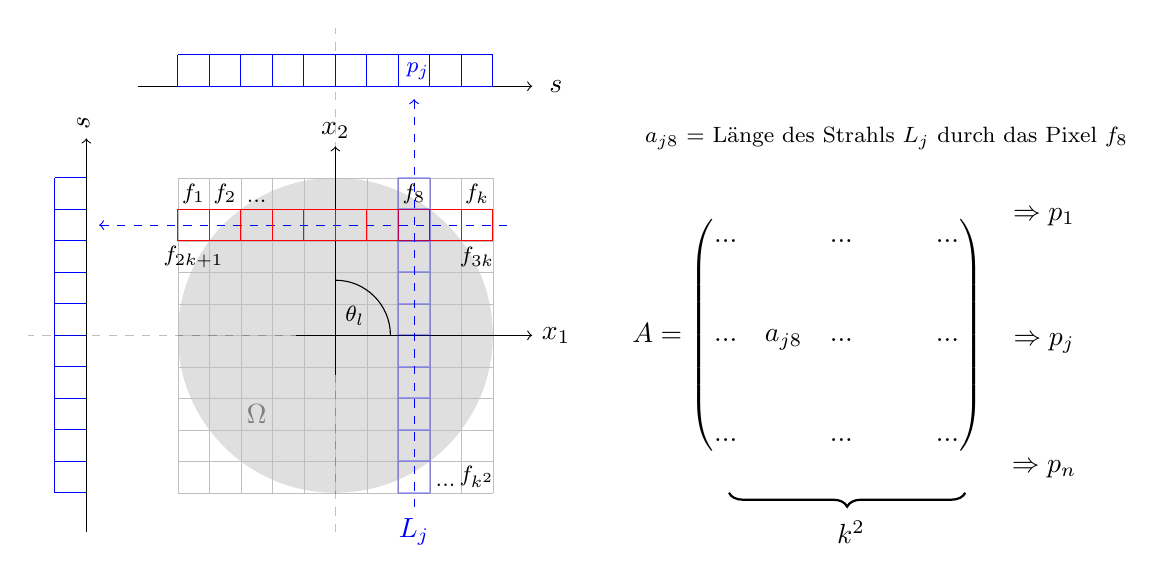
\begin{tikzpicture}
	\fill[nearly transparent, color=gray] (0,0) circle (2cm);
	\draw [gray] (-1, -1) node {$\Omega$};
	\draw [step=0.4,blue, thin, rotate=90, xshift=0, yshift=90] (-2,0) grid (2,0.4); % detector grid
	
	\draw [step=0.4, lightgray, very thin] (-2,-2) grid (2,2); % picture grid
	
	\draw [black] [->](-0.5,0) -- (2.5,0); % x-Achse
	\draw [black] (2.5, 0) node [right] {$x_1$};
	
	\draw [black] [->](0,-0.5) -- (0,2.4); % y-Achse
	\draw [black] (0, 2.6) node {$x_2$};
	
	\draw [rotate=90, xshift=0cm, <-, dashed] [blue] (1.4,3) -- (1.4,-2.2); % strahl
	%\draw [rotate=30, xshift=1.3cm ] [black] (0,-2.2) node {Röntgenstrahl};
	
	\draw [rotate=90, xshift=0, yshift=90] [black] [->] (-2.5,0) -- (2.5, 0);
	\draw [black] (2.8, 0)  node [rotate=90, xshift=2.7cm, yshift=6cm] {$s$};
	
	
	\draw [rotate=90, xshift=0cm, dashed] [nearly transparent, color=black] (0,-2.5) -- (0,3.9); % punktiert Mitte
	\draw [rotate=0, xshift=0cm, dashed] [nearly transparent, color=black] (0,-2.5) -- (0,3.9); % punktiert Mitte
	
	\draw [black] (0.7,0) arc [start angle=0, end angle=90, radius=0.7cm]; % angle \theta
	\draw [black] (0.25, 0.25) node {\footnotesize$\theta_l$};
	
	\draw [step=0.4, red, thin, rotate=90, xshift=1.2cm, yshift=0] (0,-2) grid (0.4,2);

	
	\draw [black] (0, 0)  node [rotate=0, xshift=1.4cm, yshift=-1.9cm] {\footnotesize$...$};
	\draw [black] (0, 0)  node [rotate=0, xshift=1.8cm, yshift=-1.8cm] {\footnotesize$f_{k^2}$};
		
	\draw [rotate=0, xshift=0, yshift=90] [black] [->] (-2.5,0) -- (2.5, 0);
	\draw [black] (2.8, 0)  node [rotate=0, xshift=0, yshift=90] {$s$};
	\draw [step=0.4,blue, thin, rotate=0, xshift=0, yshift=90] (-2,0) grid (2,0.4); % detector grid
	\draw [rotate=0, xshift=0cm, <-, dashed] [blue] (1,3) -- (1,-2.2); % strahl
	\draw [blue] (1,-2.5)  node {$L_j$};
	\draw [blue] (1.05,3.35)  node {\footnotesize$p_j$};
	\draw [step=0.4, blue, thick, opacity=0.3, rotate=0, xshift=0.8cm, yshift=0cm] (0,-2) grid (0.4,2);	
	
	\draw [black] (0, 0)  node [rotate=0, xshift=6cm, yshift=0cm] {$A = \begin{pmatrix}
		... & \ \ \ & ...& \ \ \ &  ... \\
		\ \ \\
		\ \ \\
		... & a_{j8} & ... & \ \ \ &  ... \\
		\ \ \\
		\ \ \\
		... & \ \ \ & ...& \ \ \ &  ... 
		\end{pmatrix}$};
	
	\draw [black] (0, 0)  node [rotate=0, xshift=9cm, yshift=1.5cm] {$\Rightarrow p_1$};
	\draw [black] (0, 0)  node [rotate=0, xshift=9cm, yshift=-0.1cm] {$\Rightarrow p_j$};
	\draw [black] (0, 0)  node [rotate=0, xshift=9cm, yshift=-1.7cm] {$\Rightarrow p_n$};	
	 
	\draw [thick,black,decorate,decoration={brace,amplitude=5pt}, rotate = 180, xshift=-6.5cm, yshift=2cm] (-1.5,0) -- (1.5,0);
	
	\draw [black] (0, 0)  node [rotate=0, xshift=-1.8cm, yshift=1.8cm] {\footnotesize$f_1$};
	\draw [black] (0, 0)  node [rotate=0, xshift=-1.4cm, yshift=1.8cm] {\footnotesize$f_2$};
	\draw [black] (0, 0)  node [rotate=0, xshift=-1cm, yshift=1.7cm] {\footnotesize$...$};
	\draw [black] (0, 0)  node [rotate=0, xshift=1cm, yshift=1.8cm] {\footnotesize$f_8$};
	\draw [black] (0, 0)  node [rotate=0, xshift=1.8cm, yshift=1.8cm] {\footnotesize$f_k$};
	\draw [black] (0, 0)  node [rotate=0, xshift=-1.8cm, yshift=1cm] {\footnotesize$f_{2k+1}$};
	\draw [black] (0, 0)  node [rotate=0, xshift=1.8cm, yshift=1cm] {\footnotesize$f_{3k}$};
	\draw [black, xshift=6.55cm, yshift=-2.5cm] (0, 0)  node {$k^2$};
	
	\draw [black, xshift=7cm, yshift=2.5cm] (0, 0)  node {\footnotesize$a_{j8}$ = Länge des Strahls $L_j$ durch das Pixel $f_8$};
	
	\end{tikzpicture}
	\caption{Eine Skizze zur Veranschaulichung des Aufbauprinzips der Abbildungsmatrix $A$ von $\mathcal{R}$.}
	\label{fig:3.9}
\end{figure}

Jetzt bleibt noch zu klären, wie das Systemmatrix $A$ initialisiert wird. In der Abbildung \ref{fig:3.9} sehen wir den Strahl $L_j$, der zu den Projektionen unter dem Winkel $\theta_1 = 0^{\circ}$ gehört. Der Strahl trifft unter anderen auch das Bildpixel $f_8$. Berechnet man die Länge des Strahls durch dieses Pixel, so kann man die errechnete Größe an der Stelle des Gewichts $a_{j8}$ in $A$ eintragen. Dementsprechend gilt es für alle betroffenen Pixel pro Strahl. 

Für jeden Winkel werden immer $k \in \N$ Projektionen erzeugt, so ergibt sich aus der Anzahl der Winkel $q \in \N$ die Anzahl der Projektionen $n = kq$, was dem Ausdruck (\ref{equa:3.1}) entspricht.   

Zu bemerken ist noch, dass die Matrix $A$ eine \textit{dünnbesetzte} Matrix ist. Mann kann leicht einsehen, dass auf der Diagonalen von $f$ maximal $\lfloor\sqrt{2}\rfloor k$ Pixel liegen. Wenn der Strahl etwas neben der Diagonalen parallel verläuft, trifft er höchstens $2\lfloor\sqrt{2}\rfloor k - 1$ Pixel von $f$; dies ist auch die maximale Anzahl der Einträge von $A$ in einer Zeile.

\begin{Bemerkung}
	Die Längen des Strahls pro Pixel zu berechnen, ist nicht die einzige Möglichkeit $A$ zu modellieren. Die Gewichte $a_{ji}$ können auch als Verhältnis der Fläche des Strahls zu der Pixelfläche aufgestellt werden. Das modelliert zwar das Abbildungssystem von $\mathcal{R}$ besser, ist aber viel rechenaufwendiger, als die hier betrachtete Vorgehensweise \cite[S. 141]{Zeng09}.
\end{Bemerkung}
Die Implementierung der Funktion zur Erstellung der Systemmatrix ist in \ref{cha:A.4} kommentiert und ist auf der beigelegten CD-ROM einzusehen.\\\\

Nachdem die Konstruktion der Systemmatrix etwas erhellt wurde, wollen wir zu der Diskussion der darauf aufbauenden Rekonstruktionsverfahren übergehen. Die sogenannten \textit{algebraische Rekonstruktionstechniken} (eng. \textit{algebraic reconstruction technique, ART}) beruhen auf der Kenntnis von $A$. Als erstes würde man wahrscheinlich auf die Idee kommen, die Gleichung $Af = p$ zu invertieren. Nun in der Regel ist $A$ sehr groß und hat keine einfache Struktur, sodass keine schnelle Inversion gefunden werden kann und wenn, dann ist es sehr zeit- und speicherintensiv (vergl. \cite[S. 157]{Burg91}). Zudem kann es vorkommen, dass $m > n$ ist, was heißen würde, dass das System unterbesetzt ist und dadurch keine eindeutige oder gar keine Lösung haben kann. Deshalb sucht man nach anderen Techniken $f$ zu rekonstruieren.

\subsection{Iterative Rekonstruktion nach Kaczmarz}
\label{cha:3.2.1}

In diesem Abschnitt wollen wir ein iteratives Verfahren zur Lösung des Gleichungssystems (\ref{equa:3.22}) nach Kaczmarz\footnote{Stefan Kaczmarz (1895-1939) polnischer Mathematiker.} anschauen. Das Verfahren kann folgendermaßen hergeleitet werden. Dafür betrachten wir (\ref{equa:3.22}) in expandierter Form
\begin{equation}
	\begin{split}
		a_{11}f_1 + \ \ \dots \ \ + a_{1m}f_m & = p_1 \\
		& \ \ \vdots\\
		a_{j1}f_1 + \ \ \dots \ \ + a_{jm}f_m & = p_j \\
	    & \ \ \vdots\\
		a_{n1}f_1 + \ \ \dots \ \ + a_{nm}f_m & = p_n.
	\end{split}
	\label{equa:3.24}
\end{equation}
So stellt jede der obigen Gleichungen eine Hyperebene $H_j = \{ f \in \R^m | \langle a_j , f \rangle = p_j, \ j \in [1,n], n \in \N  \}$ dar. Hier ist $a_j$ die $j$-te Zeile von $A$. Damit liegt die Lösung von (\ref{equa:3.24}) genau in dem Schnittpunkt aller Ebenen, was in diesem Falle $f \in \R^m$ bedeuten würde. 

Zum Suchen von $f$ bietet sich die Methode der Lotprojektion an. Dafür wählt man einen beliebigen Punkt $f_0$ und projiziert einen Lot von $f$ aus auf eine beliebige Hyperebene $H_j$. Der Schnittpunkt des Lots mit $H_j$ ist dann $f_1$. Von $f_1$ aus projiziert man auf die nächste Hyperebene, so initialisiert man $f_2$ und so weiter, bis man an dem Schnittpunkt $f$ angekommen ist (Abb. \ref{fig:3.10}). 

Dieses Vorgehen beschreibt genau die Arbeitsweise des Algorithmus, also das Kaczmarz-Verfahren. Man unterscheidet zwischen dem vorwärts projektiven Verfahren und dem randomisierten. Der Unterschied besteht nur darin, dass bei dem ersten Verfahren die Projektionen auf die Ebenen der Reihe nach berechnet werden und in dem zweiten Verfahren werden die Ebenen zufällig ausgewählt.
\begin{figure}[H]
	\centering
	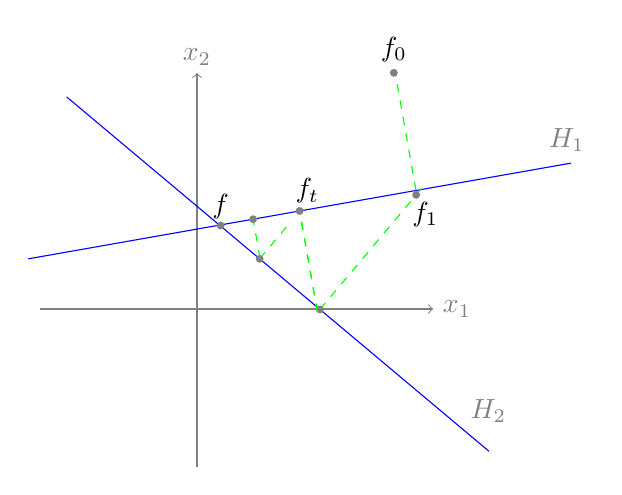
\begin{tikzpicture}
	
	\draw [gray] [->](-2,0) -- (3,0); % x-Achse
	\draw [gray] (3, 0) node [right] {$x_1$};
	
	\draw [gray] [->](0,-2) -- (0,3); % y-Achse
	\draw [gray] (0, 3.2) node {$x_2$};
	
	\draw [rotate=-40, xshift=1cm, yshift=1cm] [blue] (3,0) -- (-4,0); % blue ray	
	\draw [gray, xshift=3.7cm, yshift=-1.3cm] (0,0) node {$H_2$};
	
	\draw [rotate=10, xshift=1cm, yshift=1cm] [blue] (4,0) -- (-3,0); % blue ray
	\draw [gray, rotate=10, xshift=5cm, yshift=1.3cm] (0,0) node {$H_1$};
	
	\draw [rotate=100, xshift=1cm, yshift=-3cm, dashed] [green] (0,0) -- (1.5,0); % green from strat
	\fill[color=gray, xshift=1cm, yshift=3cm] (1.5,0) circle (0.05cm); % f point
	\draw [color=black, xshift=1cm, yshift=3cm] (1.5,0.3) node {$f_0$};
	
	\draw [rotate=50, xshift=1cm, yshift=-1.2cm, dashed] [green] (0,0) -- (2,0); % green from strat
	\fill[color=gray,rotate=50, xshift=1.4cm, yshift=-1.2cm] (1.5,0) circle (0.05cm); % f 1 point
	\draw [color=black,xshift=1.4cm, yshift=1.2cm] (1.5,0) node {$f_1$};
		
	\draw [rotate=100, xshift=-0.3cm, yshift=-1.5cm, dashed] [green] (0,0) -- (1.3,0); % green from strat	
	\fill[color=gray,rotate=50, xshift=1cm, yshift=-1.2cm] (0,0) circle (0.05cm); % f 2 point
	%\draw [color=black, xshift=1.45cm, yshift=-0.2cm] (0,0) node {$f_2$};
		
	\draw [rotate=100, xshift=-0.3cm, yshift=-1.5cm, dashed] [green] (0,0) -- (1.3,0); % green from strat	
	\fill[color=gray,rotate=100, xshift=-0.3cm, yshift=-1.5cm] (1.3,0) circle (0.05cm); % f 3 point
	\draw [color=black, xshift=0.1cm, yshift=1.5cm] (1.3,0) node {$f_t$};
	
	\draw [rotate=50, xshift=0.3cm, yshift=-0.2cm, dashed] [green] (0.7,0) -- (1.3,0); % green from strat		
	\fill[color=gray, rotate=50, xshift=0.3cm, yshift=-0.2cm] (0.7,0) circle (0.05cm); % f 4 point
	%\draw [color=black, xshift=0.1cm, yshift=0.3cm] (0.7,0) node {$f_4$};
	
	\draw [rotate=100, xshift=-0.2cm, yshift=-0.9cm, dashed] [green] (0.7,0) -- (1.3,0); % green from strat	
	\fill[color=gray, rotate=100, xshift=-0.2cm, yshift=-0.9cm] (1.2,0) circle (0.05cm); % f point
	
	\fill[color=gray, xshift=0.3cm, yshift=1.06cm] (0,0) circle (0.05cm); % f point
	\draw [color=black, xshift=0.3cm, yshift=1.3cm] (0,0) node {$f$};	
	
	\end{tikzpicture}
	\caption{Eine Veranschaulichung der Arbeitweise des Kaczmarz-Verfahrens in $\R^2$.}
	\label{fig:3.10}
\end{figure}

\begin{Bemerkung}
	Die Abbildung \ref{fig:3.10} zeigt ein Fall, wo die Lösung immer gefunden werden kann, denn der Schnittpunkt zweier Geraden ist immer exakt bestimmbar. Schon ab $\R^n$ für $n \geq 2$ ändert sich die Situation in den realen Fällen drastisch. Der Grund dafür ist, dass man ein mit Rauschen behaftetes System $Af \approx p + \epsilon$ hat. Somit ist jede Hyperebene $H_j$ um ein $\epsilon_j, \ j \in [1, n], \ n \in \N$ von dem Schnittpunkt verschoben. Das heißt, dass die Lösung $\tilde{f} \approx f$ in einem kleinem Toleranzvolumen $\prod \limits_{j=1}^{n}\epsilon_j$ liegt und daher nur annähernd angebbar ist.
	\label{be.:11}
\end{Bemerkung}

In \cite{Neufeld15} wird gezeigt, dass das randomisierte Verfahren eine schnellere Konvergenz nachweist. Aus diesem Grund werden wir dieses Vorgehen in Betracht ziehen. 
\begin{Definition}[Randomisierter Kaczmarz-Algorithmus]
	Sei $Af = p$ ein konsistentes, lineares Gleichungssystem. Sei $f_0 \in \R^m$ ein beliebiger Startwert. Für $t = 0, 1, 2, ...$ ist der Randomisierte Kaczmarz-Algorithmus definiert als
	\begin{equation}
			f_{t+1} = f_t + \frac{p_j - \langle a_j, f_t \rangle}{\parallel a_j \parallel_{2}^{2}}a_j,
			\label{equa:3.25}
	\end{equation}
	wobei $a_j$ die $j$-te Zeile von $A$ ist und $p_j$ die dazugehörige Projektion. $j$ wird zufällig ausgewählt.
	\label{def:5}	
\end{Definition} 
Wir wollen nun (\ref{equa:3.25}) etwas besser verstehen. Dafür formen wir diese Gleichung etwas um und bekommen

\[f_{t+1} = f_t + \left( \frac{p_j}{\parallel a_j \parallel_{2}} - \langle \frac{a_j}{\parallel a_j \parallel_{2}}, f_t \rangle \right) \frac{a_j}{\parallel a_j \parallel_{2}}.\]

Der eingeklammerte Teil der Gleichung stellt den Abstand von $f_t$ zu der $j$-ten Hyperebene $H_j$ in der Hesseschen Normalform Darstellung dar. Die Multiplikation mit $\frac{a_j}{\parallel a_j \parallel_{2}}$ liefert die Orthogonalität zu der $H_j$. Somit haben wir die oben beschriebene Lotprojektion, oder auch orthogonale Projektion auf $H_j$ genannt. 

Nun wollen wir uns von der Qualität des Verfahrens überzeugen, dessen genaue Implementierung in \ref{cha:A.5} (insbesondere die Abbruchbedingung (\ref{equa:A.1}) des Verfahrens) erläutert ist. Dazu sei die Abbildung \ref{fig:3.11} betrachtet. Die Ergebnisse in der Abbildung \ref{fig:3.11} wurden unter den gleichen Bedingungen, wie für die gefilterte Rückprojektion in den Abbildungen \ref{fig:3.6} für ungestörte und \ref{fig:3.8} (mittig) für gestörte Daten erzeugt. 

Man erkennt, dass die Ergebnisse der iterativen Rekonstruktion optisch gleichviel (oder sogar mehr) Informationsgehalt bieten, wie die der gefilterten Rückprojektion.
\begin{figure}[!h]
	\begin{center}
		\subfloat[\label{fig:3.11.a}Iterative Rekonstruktion aus nicht verrauschten Daten von \ref{fig:3.2.b}.]{{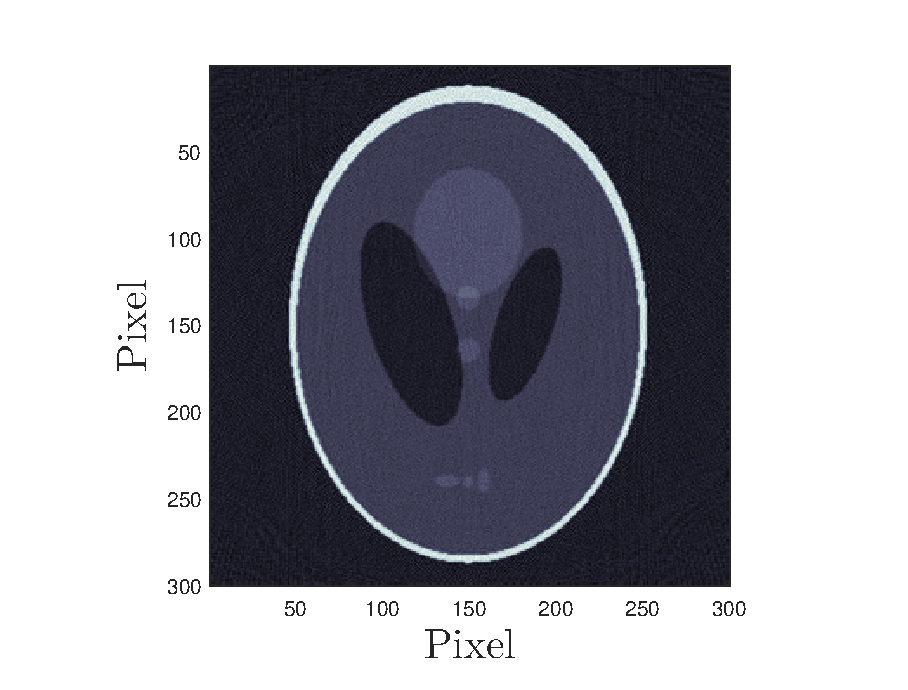
\includegraphics[width=0.5\textwidth]{iter.eps} }}
		\subfloat[\label{fig:3.11.b}Iterative Rekonstruktion aus verrauschten Daten von \ref{fig:3.7.b}]{{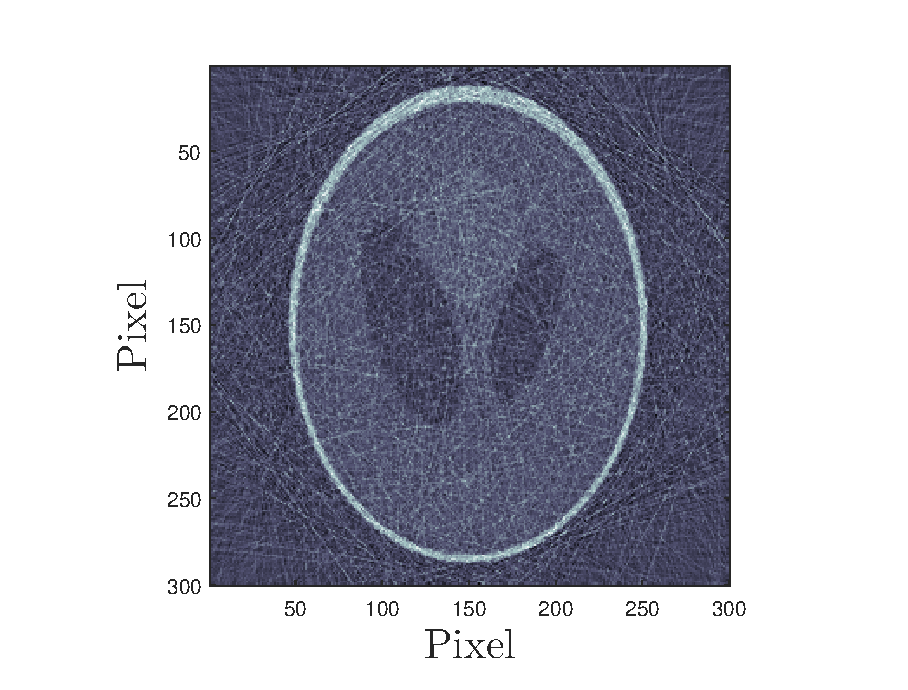
\includegraphics[width=0.5\textwidth]{iterNoised.eps} }}
	\end{center}
	\caption{Randomisierte iterative Rekonstruktionen (a) nicht verrauscht, (b) verrauscht. Die Projektionen in Beiden Fällen wurden für alle Winkel $\theta$ von $1^{\circ}$ bis $180^{\circ}$ mit der Schrittweite von $1^{\circ}$ berechnet. Detektorbreite ist $k=300$.}
	\label{fig:3.11}
\end{figure}

Jetzt wollen wir experimentell an einem Beispiel nachweisen, dass das randomisierte Verfahren in der Tat schneller konvergiert als das vorwärts projektive. Für unsere Testzwecke wählen wir ein Phantombild mit der Größe $50\times50$ Pixel (\MATLAB, \verb|phantom(50)|). Die kleine Größe des Phantombildes soll die Größe der Systemmatrix in annehmbaren Rahmen halten, da sonst zu große Matrizen entstehen, die sehr lange Rechenzeiten brauchen werden. Schließlich wollen wir nur die Konvergenz des Verfahrens untersuchen.
\begin{figure}[!h]
	\begin{center}
		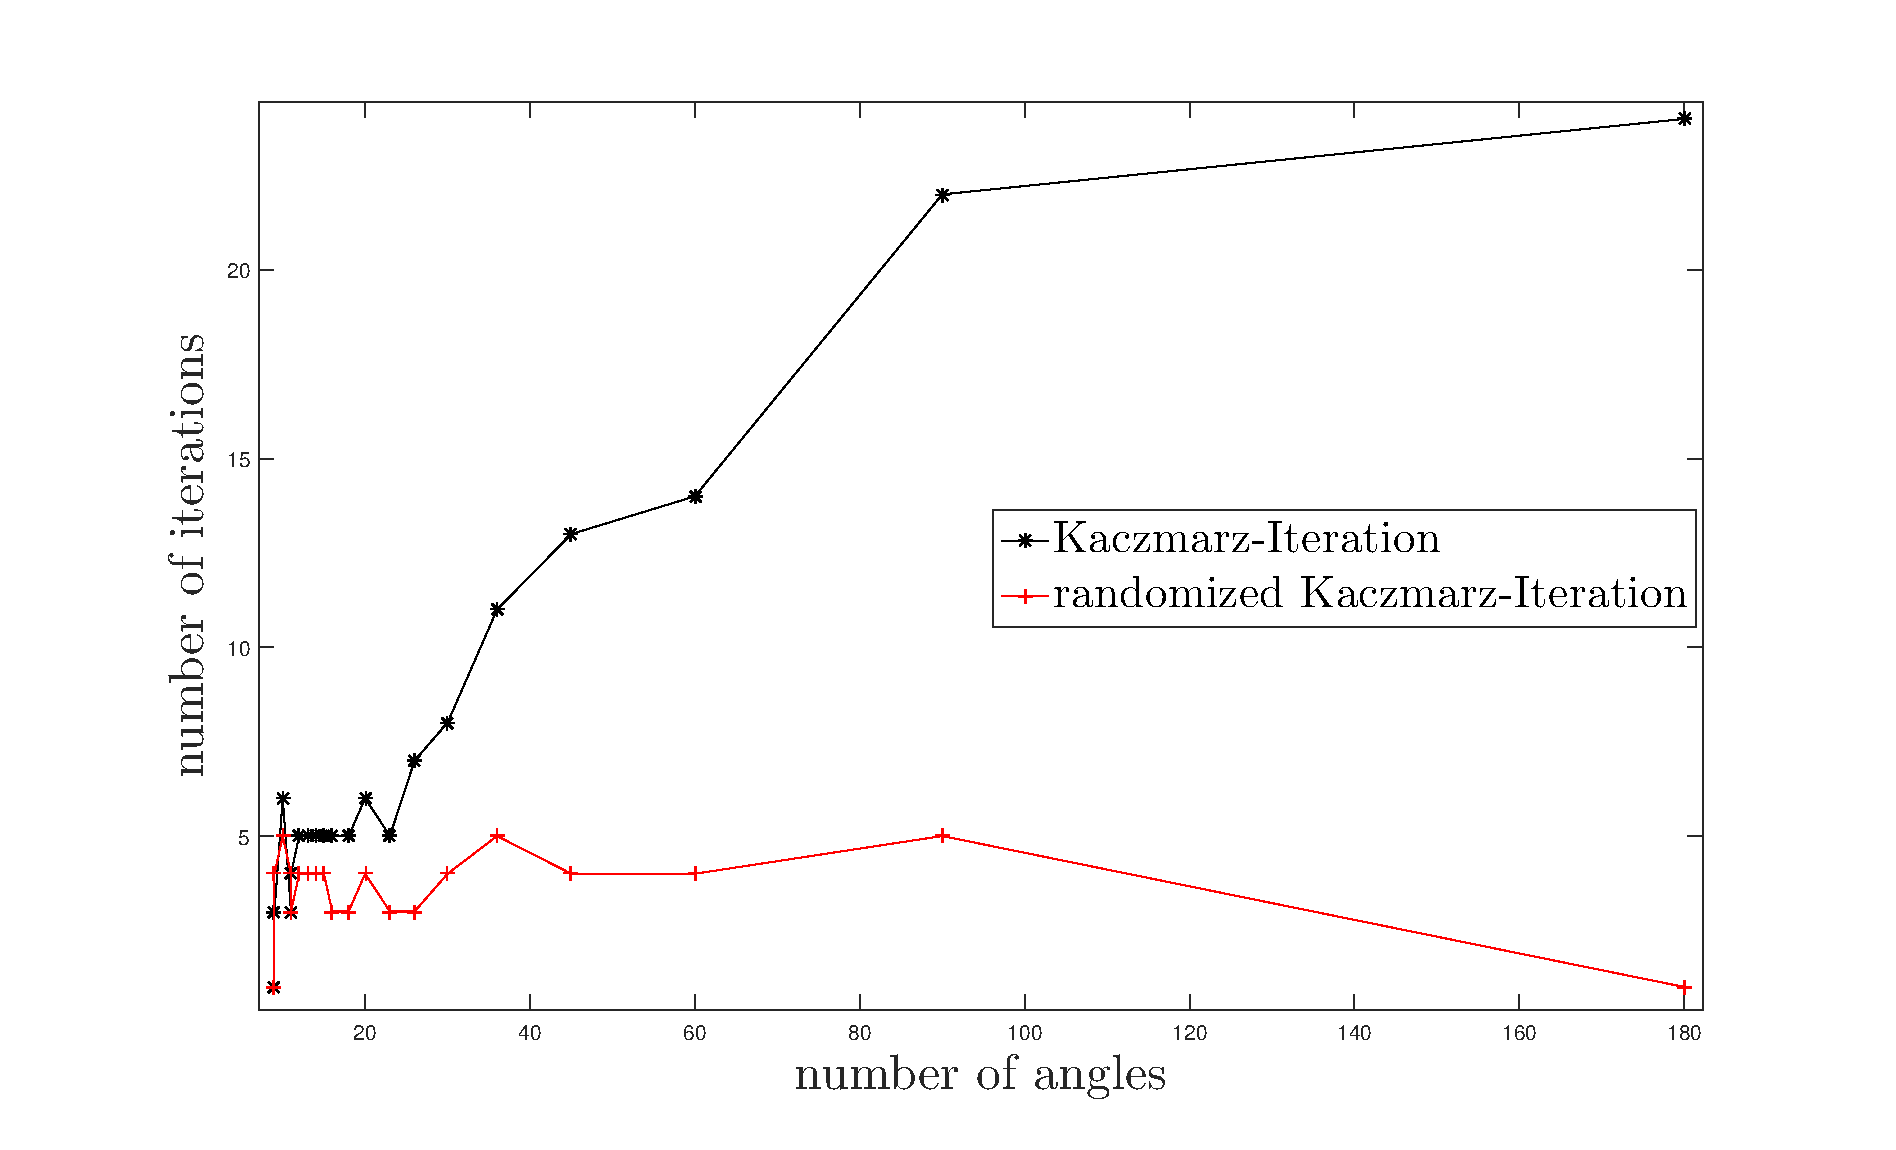
\includegraphics[width=\textwidth]{iterVSforward.eps}
	\end{center}
	\caption{Ein Vergleich des randomisierten und vorwärts projektiven Kaczmarz-Verfahrens. Der Test wurde für die Rekonstruktion eines $50 \times 50$ Pixel großen Bildes durchgeführt. In jedem Testschritt wurde die Winkelanzahl erhöht, sodass die Systemmatrix immer größer wurde.}
	\label{fig:3.12}
\end{figure}

In der Abbildung \ref{fig:3.12} ist das Ergebnis des Tests aus verrauschten (Salzstreuer-Effekt) Daten zu sehen. Dabei wurde die Systemmatrix in jedem Testschritt vergrößert, indem sich die Winkelanzahl und somit die Projektionsanzahl erhöhten. Der erste Testschritt wurde mit einer Winkelschrittweite von 20°, also für $q = 9$ Winkelpositionen durchgeführt. Die Detektorbreite wurde mit $k = 50$ initialisiert, was insgesamt für $A \in \R^{450\times2500}$ im erstem Testschritt ergeben hat. Der Test wurde bis $q = 180^{\circ}$ mit der Winkelschrittweite von 1°, das heißt bis $A \in \R^{9000 \times 2500}$ durchgeführt.

Die Abbruchbedingung musste für jeden Testschritt angepasst werden, da die Größe von $A$ schrittweise erhöht wurde und damit auch die Fehleranfälligkeit des Verfahrens. Aus (\ref{equa:A.1}) folgt $\delta = \alpha\epsilon$, wo $\epsilon = ||p - \tilde{p}||_2$ der Norm des Fehlers. $\alpha$ wurde als Verhältnis der Zeilenanzahl von $A$ im jetzt-Schritt zu davor-Schritt multipliziert mit dem Verhältnis der Winkelanzahl im jetzt-Schritt zu davor-Schritt aufgefasst. Da die Abbruchbedingung für beide Verfahren gleich war, kann man den Test als fair annehmen.

\subsection{Rekonstruktion durch SWZ}
\label{cha:3.2.2}

Das letzte Verfahren, das wir uns anschauen werden beruht auf der Singulärwertzerlegung einer Matrix. Bekanntlich besitzt jede Matrix $A \in \R^{n\times}$ (wir beschränken uns hier auf reelle Matrizen) mindestens eine SWZ, sodass $A = U\Sigma V^{*}$ geschrieben werden kann. $U \in \R^{m\times m}$ ist die \textit{unitäre} Matrix des Bildes von $A$, $\Sigma \in \R^{m \times n}$ beinhaltet die Singulärwerte von $A$ auf der Diagonale sonst überall Null und $V^*$ ist die adjungierte der unitären Matrix des Kerns von $A$. Somit lässt sich die Gleichung (\ref{equa:3.22}) in der Form 
\begin{equation}
	Af = (U\Sigma V^*)f = p
	\label{equa:3.26}
\end{equation}
schreiben. Aus der Definition der unitären Matrizen folgt $U^{-1} = U^*$ und $(V^*)^{-1} = (V^*)^* = V$. Da $\Sigma$ eine Diagonalmatrix mit Singulärwerten größer Null ist, kann $\Sigma$ wie folgt invertiert werden
\begin{equation}
	\Sigma^+ = \left\{ \begin{matrix} \frac{1}{\sigma_{ji}} & : & \mbox{falls} \ j = i \\ 0 & : & \mbox{sonst} \end{matrix}\right. .
	\label{equa:3.27}
\end{equation}
Somit kann die Gleichung (\ref{equa:3.26}) invertiert werden, also
\begin{equation}
	f = (V\Sigma^+ U^*)p.
	\label{equa:3.28}
\end{equation}
Schreibt man die Gleichung \ref{equa:3.28} in expandierter Form auf
\begin{equation}
	f_i = \sum\limits_{i = 1}^{m}[\Sigma^+]_{ii} \langle p, u_i \rangle v_i,
	\label{equa:3.29}
\end{equation}
was mit $[\Sigma^+]_{ii} = \sigma^{-1}_{i}$ genau (\ref{equa:2.3}) entspricht. 

Mit den Ergebnissen aus dem Kapitel \ref{cha:2} wissen wir, dass bereits kleine Fehler in dem Messprozess stark oszillierend auf die Lösung (\ref{equa:3.29}) wirken können. Somit bedarf es einer Regularisierung in der Rekonstruktion. Wir werden die \textit{Tikhonov\footnote{Andrei Nikolajewitsch Tichonow (1906-1993) russischer Mathematiker.}-Regularisierung} benutzen, die wie folgt aufgeschrieben werden kann:
\begin{equation}
	d_i = \frac{\sigma_i}{\lambda^2 + \sigma_i^2}.
	\label{equa:3.30}
\end{equation}
Man erkennt, dass die Regularisierung für $\lambda = 0$ keine Wirkung ergibt. Ist $\lambda \geq 0$ so wirkt die Regularisierung dämpfend auf $\sigma_i$ und verhindert bei großen Werten die Oszillation der Lösung. Wir ersetzen die Elemente auf der Diagonale von $\Sigma^+$ mit (\ref{equa:3.30}) und benennen die Matrix mit $D$
\begin{equation}
	\tilde{f}_i = \sum\limits_{i = 1}^{m}[D]_{ii} \langle p, u_i \rangle v_i.
	\label{equa:3.31}
\end{equation} 

Wir wollen unsere Untersuchungen an dem Phantom-Beispiel (\verb|phantom(50)|) weiterführen. Wie in dem vorherigen Abschnitt werden die Daten mit dem Salzstreuer-Effekt beaufschlagt, sowie anschließend auch die Messdaten. Dabei wurden die Projektionen für 50 Winkel mit der Schrittweite von 3.6° aufgenommen. Folglich bekommt man eine Systemmatrix $A \in \R^{2500 \times 2500}$.

Nun wollen wir die Wirkung der Regularisierung (\ref{equa:3.31}) auf die Reihe (\ref{equa:2.4}) aus dem Satz \ref{satz:3} an unserem Beispiel verifizieren. Zunächst lassen wir das Verfahren (\ref{cha:A.6}) für verschiedene $\lambda$ das Phantombild rekonstruieren und tragen den entstandenen Rekonstruktionsfehler $||A\tilde{f} - p ||_2$ gegen $\lambda$ in einem Diagramm auf. Das Ergebnis ist in der Abbildung \ref{fig:3.13.a} zu sehen. Zu erkennen ist, dass der minimale Fehler etwa bei $\lambda_{min} = 5.5$ liegt (Abb. \ref{fig:3.13.a}). Anschließend lassen wir die Reihe (\ref{equa:2.4}) für zwei Parameter laufen, also $\lambda = 0$ und $\lambda_{min} = 5.5$. In der Abbildung \ref{fig:3.13.b} ist deutlich zu erkennen, dass die Reihe mit regularisierten Singulärwerten schneller konvergiert als die ohne Regularisierung.
\begin{figure}[!h]
	\begin{center}
		\subfloat[\label{fig:3.13.a}Der Fehler bei der Lösung durch SWZ in abhängigkeit von dem Regularisierungsparameter $\lambda$.]{{\includegraphics[width=0.5\textwidth]{svdErr.eps} }}
		\subfloat[\label{fig:3.13.b}Veranschaulichung der Konvergenz der Reihe (\ref{equa:2.4})]{{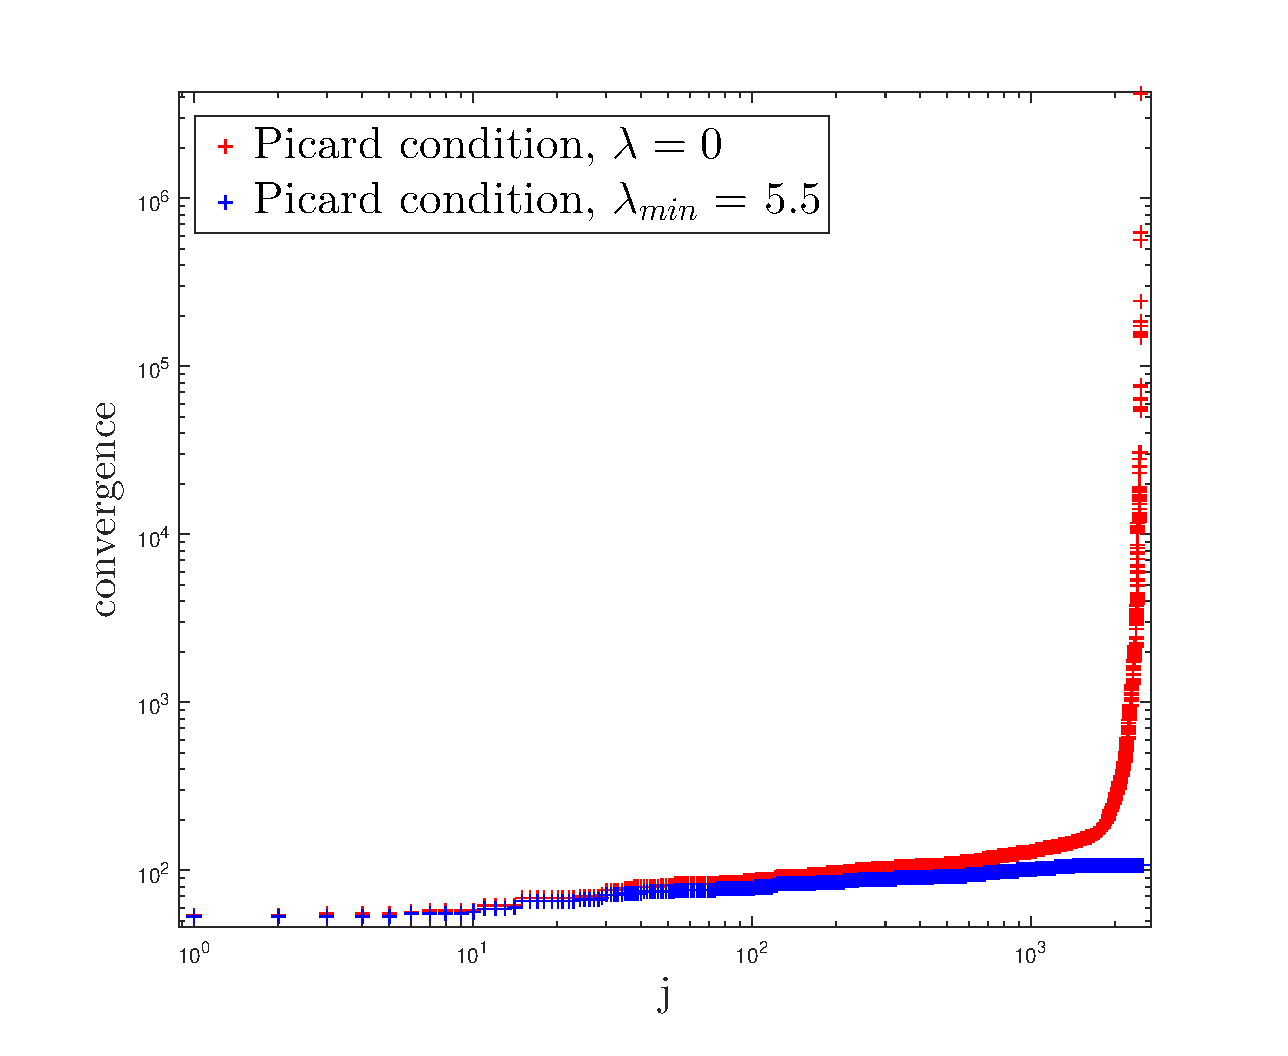
\includegraphics[width=0.5\textwidth]{picardIter.eps} }}
	\end{center}
	\caption{(a) Rekonstruktion durch SWZ, für ein Phantombild $(50\times50)$, Mit der Detektorbreite $k = 50$ und Winkelanzahl $q = 50$. (b) die  Konvergenz der Reihe (\ref{equa:2.4}) blau mit Regularisierung $\lambda_{min} = 5.5$ (das Minimum aus (a)), rot ohne Regularisierung.}
	\label{fig:3.13}
\end{figure}

\begin{figure}[!h]
	\centering
	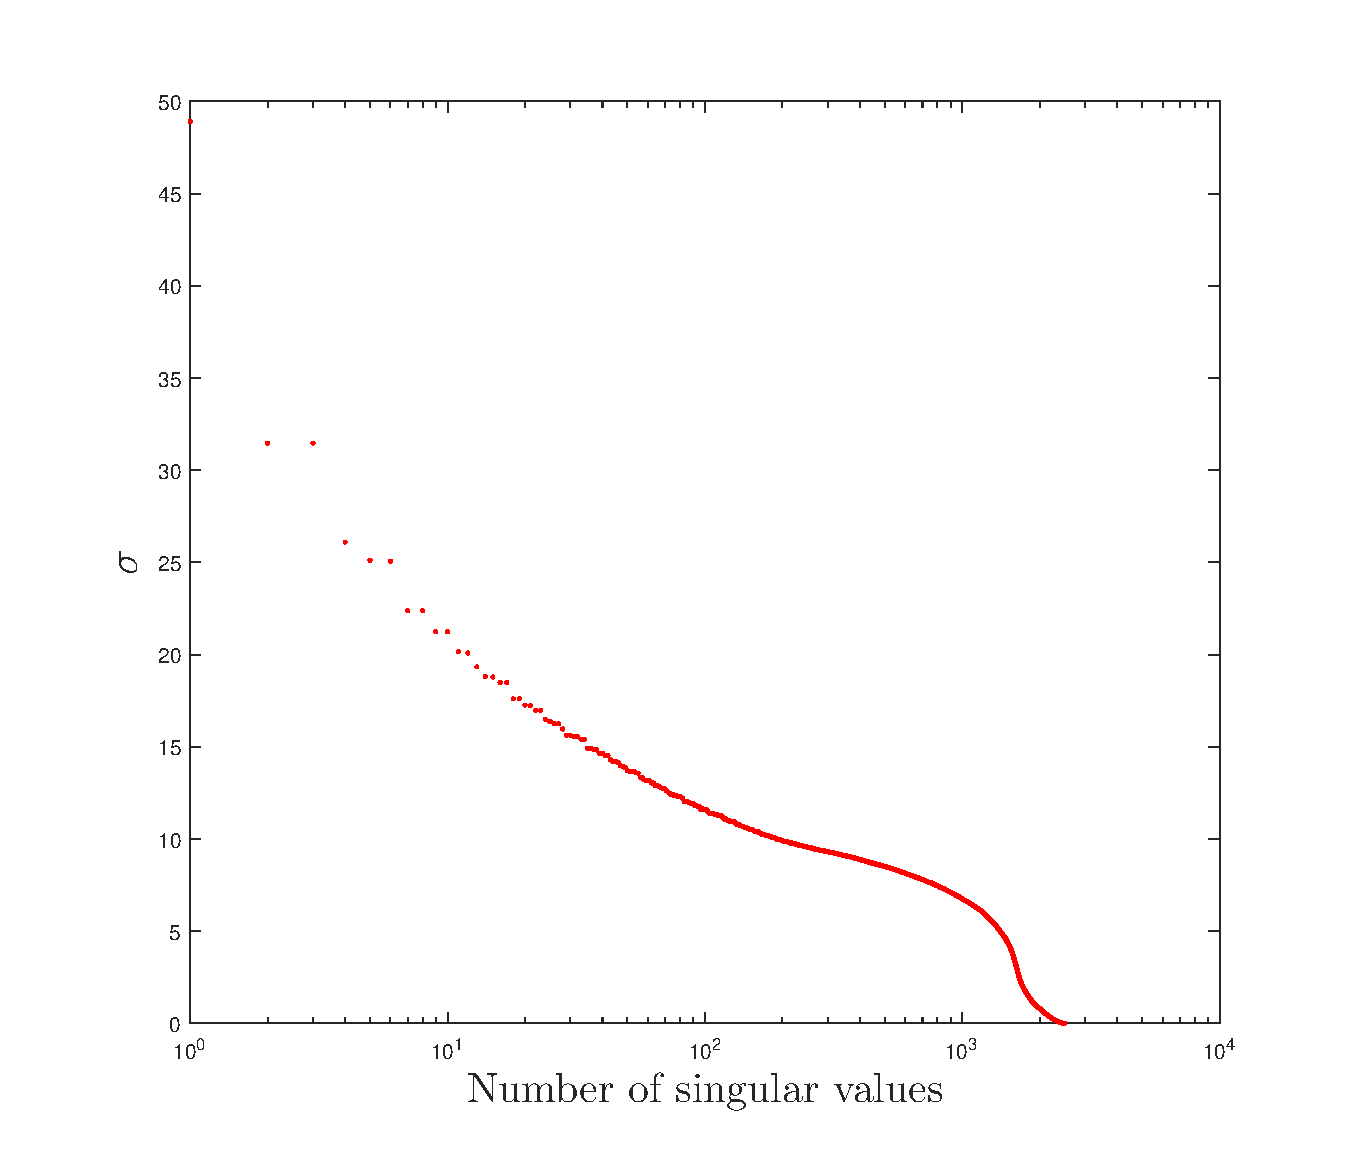
\includegraphics[width=0.5\textwidth]{singVal.eps}
	\caption{Die Folge der Singulärwerte für $A$ aus \ref{fig:3.13.a}}
	\label{fig:3.14}
\end{figure}

Insgesamt zeigt die Abbildung \ref{fig:3.13.b} die Schlechtgestelltheit des hier betrachten Problems $Af = p$ an einem konkreten Beispiel auf. Wir wissen, dass die Pcard-Bedingung (\ref{satz:3}) einen schnellen Abfall der Fourier-Koeffizienten $\langle p, u_i \rangle$ fordert, was eine stabile Lösung garantieren würde. Jedoch ist das bei Kompakten Operatoren, wie $\mathcal{R}$ ist es nie der Fall. Der Grund ist die SWZ, bei der die Singulärwerte eine abfallende Folge bilden (Abb. \ref{fig:3.14}). Was natürlich bei sehr kleinen Singulärwerten die Konvergenz der Reihe nicht fördert. Konvergiert die Reihe nicht, heißt das, dass die gemessenen Projektionen nicht in dem Bild der Operators $\mathcal{R}$ liegen. Was im Falle der verrauschten Daten garantiert ist. Durch eine passende Regularisierung ($\lambda = 5.5$) verschiebt man die verfälschten Fourier-Koeffizienten in die richtige Richtung und bekommt damit eine Minimum-Norm-Lösung. Was hier wieder zu der Abbildung \ref{fig:3.13.a} führt. Die Wirkung der Regularisierung ist in der Abbildung \ref{fig:3.15} offensichtlich.
\begin{figure}[!h]
	\centering
	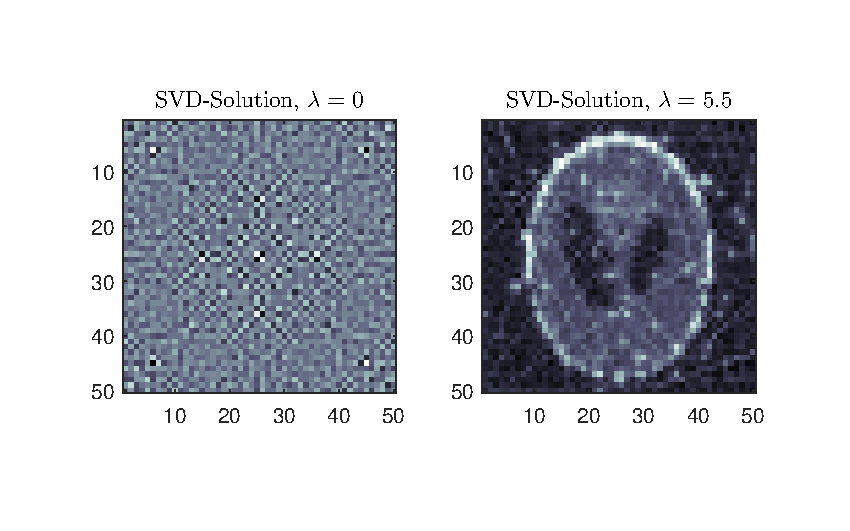
\includegraphics[width=\textwidth]{svdRedANDnotReg.eps}
	\caption{Die Rekonstruktion des Phantombildes mit der Größe $50\times50$ Pixel. Links nicht regularisiert $\lambda = 0$, recht Regularisierung mit $\lambda=5.5$.}
	\label{fig:3.15}
\end{figure}

Es ist natürlich sehr aufwendig, das Verfahren für verschiedene $\lambda$ rechnen zu lassen, um eine Minimum-Norm-Lösung zu bekommen. In der Praxis gibt es ein heuristisches Verfahren mit dem man ein optimales $\lambda_{opt}$ bestimmen kann. In der Abbildung (\ref{fig:3.14}) sehen wir, dass die Folge des Singulärwerte etwa bei $10^3$ einen Knick nach unten macht, die Singulärwerte in diesem Bereich haben den Wert zwischen 4-6. Setzt man diese Werte für $\lambda$ zu Regularisierung ein, so liefert das Verfahren die Minimum-Norm-Lösung.

%\chapter{Ausblick}
\label{cha:4}

Nach der separaten Diskussion der drei letzten Verfahren werden sie einmal miteinander verglichen. An dieser Stelle wollen wir nun auf die einzelne Vor- und Nachteile eingehen. Was für alle Verfahren zur Verbesserung vorzuschlagen ist, ist die Umstellung von Parallelstrahlgeometrie auf die Fächerstrahlgeometrie. Das würde die physikalische Eigenschaften der Röntgenstrahlen besser wiedergeben, somit würde man die sogenannte Beugung der elektromagnetischen Strahlen berücksichtigen.
\begin{figure}[!h]
	\centering
	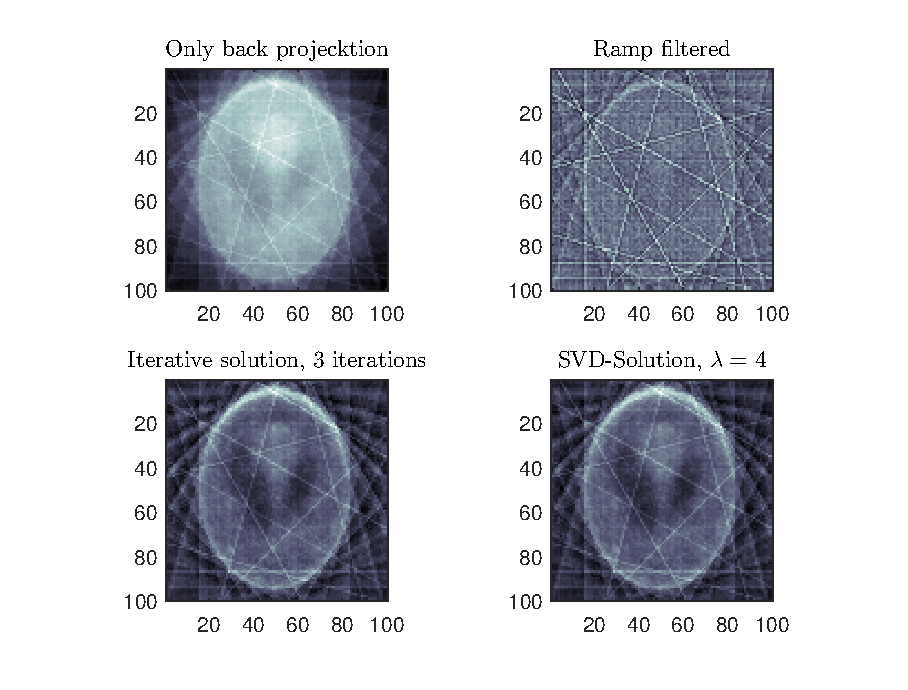
\includegraphics[width=\textwidth]{ALL.eps}
	\caption{Rekonstruktion des Phantombildes $50\times50$ Pixel. Eine Gegenüberstellung aller Verfahren in Bezug auf die Projektionsreduktion. Die Projektionen wurden nur aus 12 Winkel aufgenommen, was insgesamt $p = 1200$ ergibt.}
	\label{fig:3.16}
\end{figure}

In der Abbildung \ref{fig:3.16} ist die Empfindlichkeit der Verfahren gegenüber reduzierter Projektionenanzahl dargestellt. Dieser Aspekt ist in der medizinischen CT- Rekonstruktion von besonderem Interesse. Eine Rekonstruktion mit weniger Projektionen trägt zu einer geringeren Bestrahlungsdosis der Patienten bei. Offensichtlich sind algebraischen Verfahren in dieser Hinsicht die bessere Methoden. Allerdings sind diese für größere Auflösungen im Rekonstruktionsergebnis sehr zeit- und rechenintensiv. Somit sind es die iterativen Verfahren, die sich in der modernen medizinischen CT-Technik immer mehr durchsetzen.

Gegenüber den algebraischen Verfahren ist die gefilterte Rückprojektion sehr schnell und robust. Robust ist sie vor allem deshalb, weil sie alles filtert und zurück projiziert, was im Input reinkommt. Zudem finden dort keine Iterationen statt und es entstehen keine all zu großen Matrizen. Aber, wie die Abbildung (\ref{fig:3.16}) zeigt, ist das Verfahren für kleine Projektionenzahl sehr anfällig. Die gefilterte Rückprojektion wird heutzutage eher in der Materialforschung eingesetzt, weil dort die Strahlenbelastung der untersuchten Objekte keine große Rolle spielt und somit hohe Projektionszahlen erlaubt sind.

Zusammenfassend kann man sagen, dass für die gefilterte Rückprojektion noch mehr Filterkerne implementiert und untersucht werden könnten. Bei der Implementierung des iterativen Verfahrens, könnte noch ein 'klügerer' Fehlerschätzer überlegt werden sowie die Einführung eines Relaxationsparameters, welcher die Konvergenz des Verfahrens steigern könnte. Bei der Rekonstruktion durch SWZ wäre noch zu überlegen, wie die Singulärwerte besser gewichtet werden könnten.

%\chapter{Some More Stuff}
\label{cha:radon_trafo}




\begin{figure}[!h]
	\centering
	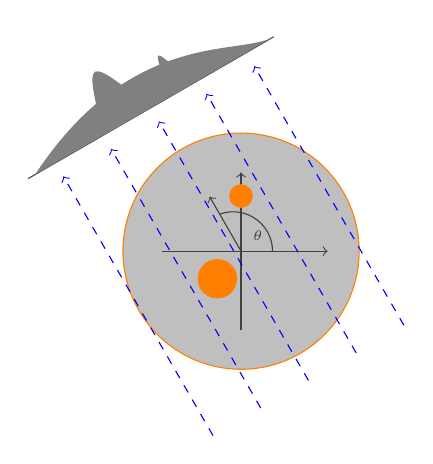
\begin{tikzpicture}[domain=3:3]  
	
	\fill[lightgray] (0.9,0) circle (1.5cm);
	
	\draw [darkgray] [->](-0.1,0) -- (2,0); % x-Achse
	%\draw (3, 0) node [right] {$x$};
	
	\draw [darkgray] [->](0.9,-1) -- (0.9,1); % y-Achse
	%\draw (0, 1.5) node [left] {$y$};
	
	%\draw (0.7, 0.2) node [right] {$\theta$};
	
	\draw [darkgray] [rotate=30, yshift=1.7cm](-1.1,0) -- (2.5,0); % s-Achse
	\draw [darkgray] [rotate=120, xshift=-1.45cm, yshift=-.78cm][->](1,0) -- (1.8,0); % s-Achse
	%\draw (1.4, 0)  node [yshift=3.7cm, right]    {$s$};
	%\draw  (0, 1.3) node [rotate=30, yshift=1.7cm] { Detektor};
	
	\draw [darkgray] (1.3,0) arc [start angle=0, end angle=110, radius=.5cm];
	\draw [darkgray](1.3, 0.2) node [left] {\tiny $\theta$};
	
	\fill[gray] [rotate=30, yshift=1.7cm] (-1,0) .. controls (1,1) and (2,0) .. (2.5,0);
	\fill[gray] [rotate=30, yshift=1.7cm] (0,0) .. controls (0.3,1)  .. (0.7,0);
	\fill[gray] [rotate=30, yshift=1.7cm] (1,0) .. controls (1.1,0.7)  .. (1.3,0);
	
	\draw[orange] (0.9,0) circle (1.5cm);
	\fill[orange] (0.9,  0.7) circle (.15cm);
	\fill[orange] (0.6, -0.35) circle (.25cm);
	%\draw (3.5, 1.1) node [left] {$f(x,y)$};
	
	%\draw[->] (0,0) -- (1.5, 0.7);
	%\draw (1.5, 0.7)  node [right] {$s$};
	
	\draw [rotate=30, dashed, ->] [blue] (0,-2.3) -- (0,1.5); % strahl
	\draw [rotate=30, xshift=-0.7cm, dashed, ->] [blue] (0,-2.3) -- (0,1.5); % strahl
	\draw [rotate=30, xshift=0.7cm, dashed, ->] [blue] (0,-2.3) -- (0,1.5); % strahl
	\draw [rotate=30, xshift=1.4cm, dashed, ->] [blue] (0,-2.3) -- (0,1.5); % strahl
	\draw [rotate=30, xshift=2.1cm, dashed, ->] [blue] (0,-2.3) -- (0,1.5); % strahl
	
	%\draw  (1.5,-1.4) node [rotate=30, yshift=-1cm, -] { Röntgenröhre};
	
	%\draw (1.55, -1.5)  node [right] {$I(s)$};
	%\draw (0.6, 1.7)  node [right] {$I(s + \Delta s)$};
	
	\begin{scope}[xshift=1cm]
	\end{scope}
	
	\end{tikzpicture}
	\caption{Schematischer Aufbau eines Computertomographen}
	\label{fig:5}
\end{figure}


\begin{figure}[!h]
	\centering
	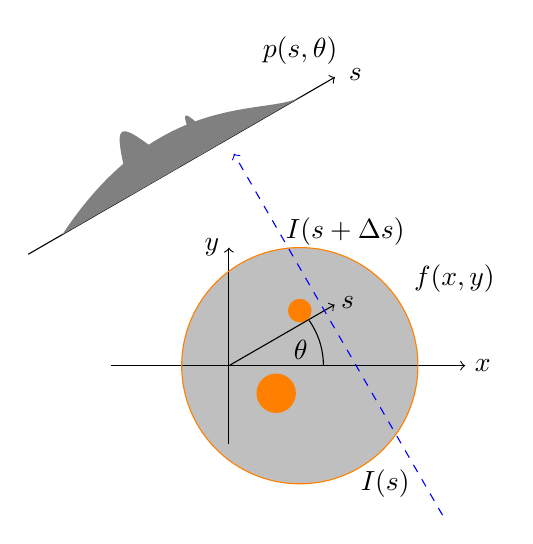
\begin{tikzpicture}[domain=3:3]  
	
	\fill[lightgray] (0.9,0) circle (1.5cm);
	
	
	\draw [->](-1.5,0) -- (3,0); % x-Achse
	\draw (3, 0) node [right] {$x$};
	
	\draw [->](0,-1) -- (0,1.5); % y-Achse
	\draw (0, 1.5) node [left] {$y$};
	
	\draw (0.7, 0.2) node [right] {$\theta$};
	
	\draw [rotate=30, yshift=2.5cm, ->](-1.5,0) -- (3,0); % s-Achse
	\draw (1.4, 0)  node [yshift=3.7cm, right]    {$s$};
	
	\draw (1.2,0) arc [start angle=0, end angle=35, radius=1cm];
	\draw (1.5, 4) node [left] {$p(s, \theta)$};
	
	\fill[gray] [rotate=30, yshift=2.5cm] (-1,0) .. controls (1,1) and (2,0) .. (2.5,0);
	\fill[gray] [rotate=30, yshift=2.5cm] (0,0) .. controls (0.3,1)  .. (0.7,0);
	\fill[gray] [rotate=30, yshift=2.5cm] (1,0) .. controls (1.1,0.7)  .. (1.3,0);
	
	\draw[orange] (0.9,0) circle (1.5cm);
	\fill[orange] (0.9,  0.7) circle (.15cm);
	\fill[orange] (0.6, -0.35) circle (.25cm);
	\draw (3.5, 1.1) node [left] {$f(x,y)$};
	
	\draw[rotate=30, ->] (0,0) -- (1.55, 0);
	\draw (1.3, 0.8)  node [right] {$s$};
	
	%\draw [rotate=30, dashed, ->] [blue] (0,-3) -- (0,2.3); % strahl
	%\draw [rotate=30, xshift=-0.7cm, dashed, ->] [blue] (0,-3) -- (0,2.3); % strahl
	%\draw [rotate=30, xshift=0.7cm, dashed, ->] [blue] (0,-3) -- (0,2.3); % strahl
	\draw [rotate=30, xshift=1.4cm, dashed, ->] [blue] (0,-3) -- (0,2.3); % strahl
	%\draw [rotate=30, xshift=2.1cm, dashed, ->] [blue] (0,-3) -- (0,2.3); % strahl
	
	\draw (1.55, -1.5)  node [right] {$I(s)$};
	\draw (0.6, 1.7)  node [right] {$I(s + \Delta s)$};
	
	
	\end{tikzpicture}
	
	\caption{Schematischer Aufbau eines Computertomographen}
	\label{fig:510}
\end{figure}

Radon\footnote{\label{foot:20} Johann Karl August Radon (1887-1956) österreichischer Mathematiker.}


\begin{equation}
	\begin{xy}
	\xymatrix{
		& L^2(\Omega) \ar@<2pt>[dl]_{\tilde{\mathcal{R}^*}} \ar@<2pt>[rd]^{\mathcal{R}} & \\
		L^2(Z, \frac{1}{\gamma(s)}) \ar@<2pt>[ru]_{\tilde{\mathcal{R}}} \ar@<2pt>[rr]^{\psi} &    & L^2(Z) \ar@<2pt>[lu]^{\mathcal{R}^*} \ar@<2pt>[ll]^{\psi^{-1}}
	}
	\end{xy}
\end{equation}




\newpage
\section{Anhang}

\begin{theorem}
	Der Satz von foo!
\end{theorem}
\begin{theorem}
	Der Satz von bar!
	\label{thm:foo}
\end{theorem}
\begin{proof}
	Beweis fertig.
\end{proof}
\begin{proof}[Beweis von Satz~\ref{thm:foo}]
	Beweis erbracht.
\end{proof}


\begin{Bemerkung}
	Der Satz von foo!
	
\end{Bemerkung}






%\chapter{Die Abschlussarbeit}
\label{cha:Diplomschrift}

Jede Abschlussarbeit%
\footnote{Die meisten der folgenden Bemerkungen gelten gleichsam für Bachelor-, Master- und Diplomarbeiten.} 
ist anders und dennoch sind sich gute
Arbeiten in ihrer Struktur meist sehr ähnlich, \va\ bei
technisch-natur\-wissen\-schaft\-lichen Themen. 

\section{Elemente der Abschlussarbeit}

Als Startpunkt bewährt hat sich die folgender
einfacher Grundaufbau, den man natürlich vari\-ieren und beliebig
verfeinern kann:
%
\begin{enumerate}
\item \textbf{Einführung und Motivation}: Was ist die Problem- oder Aufgabenstellung und
warum sollte man sich dafür interessieren?
\item \textbf{Präzisierung des Themas}: Hier beschreibt man den aktuellen Stand der Technik
oder Wissenschaft ("`State-Of-The-Art"'), zeigt bestehende
Defizite oder offene Fragen auf und entwickelt daraus die
Stoßrichtung der eigenen Arbeit.
\item \textbf{Eigener Ansatz}: Das ist natürlich der Kern der Arbeit. Hier
wird gezeigt, wie man die vorher beschriebene Aufgabenstellung löst und --
häufig in Form eines Programms%
\footnote{\emph{Prototyp} ist in diesem Zusammenhang ein gerne benutzter Begriff, der im Deutschen
allerdings oft unrichtig dekliniert wird. Richtig ist: der \emph{Prototyp}, des \emph{Prototyps}, dem/den \emph{Protototyp} -- falsch hingegen \zB: des \emph{Prototyp\underline{en}}!
} --
realisiert, ergänzt durch illustrative Beispiele.
\item \textbf{Zusammenfassung}: Was wurde erreicht und welche Ziele sind
noch offen geblieben, wo könnte man weiter arbeiten?
\end{enumerate}
%
Natürlich ist auch ein gewisser dramaturgischer Aufbau der Arbeit
wichtig, wobei man bedenken muss, dass der Leser in der Regel nur
wenig Zeit hat und -- anders als etwa bei einem Roman -- seine
Geduld nicht auf die lange Folter gespannt werden darf. Erklären
Sie bereits in der Einführung (und nicht erst im letzten Kapitel),
wie Sie an die Sache herangehen, welche Lösungen Sie vorschlagen
und wie erfolgreich Sie damit waren.

Übrigens, auch Fehler und Sackgassen darf (und sollte) man
beschreiben; ihre Kenntnis hilft oft doppelte Experimente und
weitere Fehler zu vermeiden und ist damit sicher nützlicher als
jede Schönfärberei.
Und natürlich ist es auch nicht verboten, seine eigene Meinung 
in sachlicher Form zu äußern.


\section{Arbeiten in Englisch}
\label{sec:englisch}

Diese Vorlage ist zunächst darauf abgestellt, dass die
Diplomschrift in deutscher Sprache erstellt wird. Vor allem bei
Diplomarbeiten, die in Zusammenarbeit mit größeren Firmen oder
internationalen Instituten entstehen, ist es häufig erwünscht,
dass die Diplomschrift zu besseren Nutzbarkeit in englischer
Sprache verfasst wird, und viele Hochschulen%
\footnote{Die FH Hagenberg macht hier keine Ausnahme. 
Der Begriff "`Fachhochschule"' wird dabei entweder gar nicht
übersetzt oder -- wie im deutschsprachigen Raum mittlerweile üblich -- 
mit \emph{University of Applied Sciences}.
%Die offizielle englische Übersetzung von "`Medientechnik und -design"'
%ist übrigens \emph{Media Technology and Design}.
} 
lassen dies in
der Regel auch zu.

Beachten sollte man allerdings, dass das Schreiben dadurch nicht
einfacher wird, auch wenn einem Worte und Sätze im Englischen
scheinbar leichter "`aus der Feder"' fließen. Gerade im Bereich
der Informatik erscheint durch die Dominanz englischer
Fachausdrücke das Schreiben im Deutschen mühsam und das Ausweichen
ins Englische daher besonders attraktiv. Das ist jedoch
trügerisch, da man die eigene Fertigkeit in der Fremdsprache
(trotz der meist langjährigen Schulbildung) häufig überschätzt.
Prägnanz und Klarheit gehen leicht verloren und bisweilen ist das
Resultat ein peinliches Gefasel ohne Zusammenhang und soliden
Inhalt. Sofern man das Englische nicht wirklich gut beherrscht, ist
es ratsam, zumindest die wichtigsten Teile der Arbeit zunächst in
Deutsch zu verfassen und erst nachträglich zu übersetzen.
Besonders vorsichtig sollte man bei der Übersetzung von scheinbar
vertrauten Fachausdrücken sein. Zusätzlich ist es immer zu
empfehlen, die fertige Arbeit von einem "`native speaker"'
korrigieren zu lassen.



Technisch ist, außer der Spracheinstellung und den
unterschiedlichen Anführungszeichen (s.\
Abschn.~\ref{sec:anfuehrungszeichen}), für eine englische Arbeit
nicht viel zu ändern, allerdings sollte man folgendes beachten:
%
\begin{itemize}
\item  Die Titelseite (mit der Bezeichnung "`Diplomarbeit"' oder "`Masterarbeit"') 
ist für die einzureichenden Exemplare jedenfalls in \emph{deutsch} zu halten,
auch wenn der Titel englisch ist. 
\item Ebenso muss neben dem
englischen \emph{Abstract} auch eine deutsche \emph{Kurzfassung}
enthalten sein. %
\item Akademische Titel von Personen haben im Englischen offenbar
weniger Bedeutung als im Deutschen und werden daher meist
weggelassen.
\end{itemize}

%\chapter{Zum Arbeiten mit \latex}
\label{cha:ArbeitenMitLatex}



\section{Start}
\label{sec:latex}



\latex ist eine in den Naturwissenschaften sehr verbreitete
und mittlerweile klassische Textverarbeitungssoftware für das Erstellen
großer und komplizierter Dokumente mit professionellem Anspruch.
Das Arbeiten mit \latex erscheint -- zumindest für den ungeübten Benutzer -- %
zunächst schwieriger als mit herkömmlichen Werkzeugen für die
Textverarbeitung.

Zum Ersten ist -- im Unterschied zu den meisten gängigen
Text\-ver\-arbei\-tungs\-prog\-ram\-men -- \latex nicht \textsc{Wysiwyg}%
\footnote{"`What You See Is What You Get."' Es gibt auch 
\textsc{Wysiwyg}-Implementierungen für \latex, 
\zB\ \emph{Scientific WorkPlace} (\url{www.mackichan.com}) oder
\emph{LyX} (\url{www.lyx.org}), 
die aber teuer \bzw\ relativ langsam sind.},
sondern es handelt sich um eine \emph{Markup Lang\-uage} (wie HTML) -- noch dazu
eine für den Anfänger recht komplizierte -- und zugehörige Werkzeuge.
Ungewohnt erscheinen sicher auch die vermeintlich starken
Einschränkungen von \latex,
insbesondere in Bezug auf die Wahl der Schriften und das
Layout. Während man anfangs meint, dass diese Rigidität
die eigene Kreativität beschränkt, bemerkt man mit der Zeit, dass es gerade
dadurch gelingt, sich stärker auf die Inhalte der Arbeit zu
konzentrieren als auf deren äußere Form. Dass am Ende die Form dennoch stimmt,
ist allerdings nur dann gewährleistet, wenn man sich bei den eigenen Modifikationen
der Formate und Parameter äußerste Zurückhaltung auferlegt, es sei denn,
man ist in der Zwischenzeit bereits selbst zum \latex-\emph{Guru} avanciert.

Insgesamt lohnt sich der Aufwand, wie viele meinen, zumal die Diplomarbeit
in jedem Fall (mit oder ohne \latex) ein substantielles Stück Arbeit ist.
Allerdings sollte mithilfe von \latex ein professionell aussehendes
Ergebnis einfacher zu erreichen sein und man wird sich wohl auch einigen
Ärger mit Fehlern und Einschränkungen gängiger Software ersparen.
Zudem könnte es durchaus sein, dass man nebenbei auch sein Auge für
die Feinheiten des Buchsatzes (weiter-){\optbreaknh}entwickelt.%
\footnote{Dieses abschließende Textelement wurde übrigens zur Ermöglichung eines 
Zeilenumbruchs nach der Klammer so gesetzt: \texttt{\ldots (weiter-)\{{\bs}optbreaknh\}entwickelt.}
Das Makro \texttt{{\bs}optbreaknh} ("`optional break with no hyphen"') ist in 
\texttt{hgb.sty} definiert.}


\subsection{Software}

Zum Arbeiten mit \latex benötigt man -- neben einem Computer -- natürlich Software. Musste man sich früher oft die einzelnen Komponenten von \latex mühevoll zusammensuchen und für die eigene Umgebung konfigurieren, gibt es mittlerweile für die wichtigsten Plattformen (Windows, Mac~Os, Linux) fertige \latex-Installationen, die ohne weiteres Zutun laufen. Die aktuelle Version von \latex\ ist \LaTeXe\ (sprich "`LaTeX zwei e"'). 
Zum Arbeiten mit \latex\ benötigt man zwei Dinge:
%
\begin{itemize}
\item \latex-Installation (Distribution)
\item Texteditor oder Autorenumgebung (Frontend)
%\item PostScript/PDF-Software 
\end{itemize}
%
Sämtliche Komponenten sind kostenlos und für alle gängigen Plattformen verfügbar.


\subsubsection{Windows}
\label{sec:Windows}

Unter \emph{Windows} (XP, Win7) hat sich folgendes Setup bewährt,
mit dem \ua auch dieses Dokument erstellt wurde:
%
\begin{itemize}
\item \textbf{\latex-Distribution}: \emph{MikTeX 2.9} oder höher.
MikTeX%
\footnote{\url{www.miktex.org}}
enthält auch alle notwendigen Hilfsprogramme, wie beispielsweise {\tt bibtex}.

\item \textbf{PDF-Viewer}: \emph{SumatraPDF}%
\footnote{\url{http://blog.kowalczyk.info/software/sumatrapdf/}}

\item \textbf{Frontend}: \emph{TeXnicCenter}.%
\footnote{\url{www.texniccenter.org}}
Grundsätzlich kann man jeden Text-Edi\-tor%
\footnote{Unter Windows \zB\ \emph{Ultra\-Edit} (\url{www.ultraedit.com}) oder \emph{WinEdit} (\url{www.winedit.com}).}
verwenden, praktischer ist jedoch eine integrierte \latex-Um\-geb\-ung wie TeXnicCenter, die einen auch bei 
der Dateiverwaltung, der Verarbeitung der Dokumente und der Fehlerbehandlung unterstützt.
Eine interessante Alternative ist die Verwendung von \emph{Eclipse}\footnote{\url{www.eclipse.org}}
als plattformunabhängiges Frontend 
(mit dem \emph{TeXlipse}\footnote{\url{http://texlipse.sourceforge.net/}} Plugin).
\end{itemize}
%
Beim erstem Mal sollten \emph{MikTeX}, \emph{SumatraPDF} und \emph{TeXnicCenter} in genau dieser Reihenfolge installiert werden.


\subsubsection{Mac~OS}
\label{sec:MacOs}

Unter Mac~OS~X ist die Referenzdistribution \emph{MacTeX}.%
\footnote{\url{http://www.tug.org/mactex}} 
Sie enthält neben der TeX-Distribution \emph{TeX Live} auch gängige Editoren wie \emph{TeXWorks} oder \emph{TeXshop}. Mit dem \emph{TeX Live Utility} können Pakete verwaltet und die Distribution auf den neuesten Stand gebracht werden. Als Alternative zu den beiden genannten Editoren steht \emph{TeXnicle}%
\footnote{\url{http://www.bobsoft-mac.de/texnicle/texnicle.html}} zur Verfügung. Er bietet -- ähnlich wie \emph{TeXnicCenter} unter Windows -- einen projektbasierten Workflow an.
Ein PDF-Viewer muss unter Mac~OS~X übrigens nicht extra installiert werden. Alle genannten Editoren beinhalten eine eigene PDF-Vorschau.

%ALT:
%Bewährte und weit verbreitete Frontends für den Mac sind \emph{MacTeX}%
%\footnote{\url{www.tug.org/mactex} -- enthält eine komplette und fertig konfigurierte LaTeX-Installation 
%für Mac~OS (ca.\ 1.15 GB download).}
%und \emph{TeXShop},%
%\footnote{\url{www.uoregon.edu/~koch/texshop/}}
%das üblicherweise zusammen mit der TeX-Distribution \emph{TeX Live} verwendet wird. 
%Weit verbreitet ist auch der \emph{TeXworks} Editor, der ebenfalls im MacTeX Package enthalten ist und auch MiKTeX unter Windows beigefügt ist.


\subsubsection{Linux}

Auch unter Linux ist \emph{TeX Live} (\so) eine häufig verwendete TeX-Distri\-bution. 
Als Frontend sind beispielsweise
\emph{Lyx}\footnote{\url{www.lyx.org}},
\emph{Kile}\footnote{\url{http://kile.sourceforge.net}} und
\emph{Texmaker}\footnote{\url{www.xm1math.net/texmaker/}} 
verbreitet.
In manchen gängigen Linux-Versionen ist bereits eine komplette \latex-Distribution enthalten, sodass im besten Fall überhaupt keine zusätzliche Installation notwendig ist.  


\subsection{Literatur}
\label{sec:literatur}

Es ist müßig, ohne geeignete Literatur mit \latex zu beginnen, selbst
als fortgeschrittener Benutzer wird man immer wieder auf Hilfe angewiesen
sein. Erfreulicherweise ist sehr viel Nützliches auch online verfügbar.
Gute Startpunkte sind \zB
%
\begin{itemize}
\item \emph{{\rm\LaTeXe}-Kurzbeschreibung} von Schmidt et al.\ \cite{Schmidt01}
\item \emph{The Not So Short Introduction to {\rm \LaTeXe}}
            von Oetiker et al.\ \cite{Oetiker01}
\end{itemize}
%
\noindent
Als mittlerweile bereits klassisches Handbuch zu \latex ist
%
\begin{itemize}
  \item \emph{A Guide to {\rm\LaTeXe}} von H.~Kopka und P.~Daly \cite{Kopka98}
\end{itemize}
%
zu empfehlen, zu dem es für Interessierte auch zwei vertiefende
Zusatzbände in Deutsch gibt. Zahlreiche weitere Dokumente zu
\latex und verwandten Themen finden sich \ua im Rahmen des {\em
Comprehensive TeX Archive Network} (CTAN) auf
\begin{quote}
	\url{www.ctan.org}%
	\footnote{\url{www.ctan.org/tex-archive/help/Catalogue/bytopic.html}}\newline
	\url{http://dante.ctan.org}%
	\footnote{\url{http://dante.ctan.org/tex-archive/help/Catalogue/bytopic.html}}\newline
	\url{www.tex.ac.uk}
\end{quote}
%
Besonders nützlich sind auch die
\emph{Comprehensive List of {\rm \latex} Symbols} \cite{Pakin01}
und die Beschreibungen wichtiger \latex-Pakete, wie
%
\begin{quote}
	\texttt{babel} \cite{Braams2008},\newline
% \texttt{german}, \texttt{ngerman} \cite{Raichle98},\newline
  \texttt{grahics}, \texttt{graphicx} \cite{Carlisle99},\newline
  \texttt{fancyhdr} \cite{Oostrum97},\newline
  \texttt{caption} \cite{Sommerfeldt07},\newline
  \texttt{subfigure} \cite{Cochran95}.
\end{quote}





\section{Schrift}

\subsection{Schriftarten}

\latex verwendet normalerweise die Schriften der \emph{Computer
Modern}
(CM) Serie, die so wie die \emph{TeX}-Software selbst von Donald Knuth%
\footnote{\url{www-cs-staff.stanford.edu/~knuth/}} entwickelt
wurden. Die drei Basis-Schrifttypen der CM-Serie in \latex sind
%
\begin{quote}
\begin{tabular}{lcl}
\textrm{Roman}      & & \verb!\textrm{Roman}!\\
\textsf{Sans Serif} & & \verb!\textsf{Sans Serif}!\\
\texttt{Typewriter} & & \verb!\texttt{Typewriter}!\\
\end{tabular}
\end{quote}
%
\noindent In den Augen vieler Benutzer ist allein die Qualität und
Zeitlosigkeit dieser Schriften ein Grund, \latex für seriöse
Zwecke zu verwenden. Ein weiterer Vorteil der \emph{TeX}-Schriften
ist, dass die unterschiedlichen Schriftfamilien und Schnitte
bezüglich der Größe sehr gut aufeinander abgestimmt sind.

Darüber hinaus können aber in \latex auch beliebige 
\emph{PostScript}-Schrif\-ten (Type 1) verwendet werden, was allerdings in
der Praxis einiges an "`Tuning"'-Arbeit verlangt. Häufig verwendet
werden \zB\ \emph{Times} und \emph{Palatino}, derzeit ist aber ein Trend 
zurück zu den klassischen CM-Schriften zu beobachten.



\subsection{Texte hervorheben}

Texte können auf unterschiedliche Weise aus dem Fließtext hervorgehoben werden.
\begin{itemize}
%
\item Die Auszeichnung in \textit{Kursivschrift} oder "`italic"' (\verb!\textit{..}!) ist \va\ zum Hervorheben von
Betonungen und Zitaten geeignet, aber auch für
Produktbezeichnungen, Fremdwörter und Variablen im Text, \zB
%
\begin{quote}
\verb!\textit{Variable}! $\rightarrow$ \textit{Variable}
\end{quote}
%
\item {\sl Slanted} %
(\verb!\textsl{..}!) bedeutet eine geneigte Schrift und
unterscheidet sich damit deutlich von \textit{Italic}. Wird
beispielsweise verwendet für die laufenden Kopfzeilen,
Produktbezeichnungen und Markennamen -- zum Vergleich:
%
\begin{quote}
\verb!\textrm{Daimler-Chrysler}! $\rightarrow$ \textrm{Daimler-Chrysler} \newline%
\verb!\textsl{Daimler-Chrysler}! $\rightarrow$ \textsl{Daimler-Chrysler} \newline%
\verb!\textit{Daimler-Chrysler}! $\rightarrow$ \textit{Daimler-Chrysler}
\end{quote}
%
\item \textbf{Boldface} (\verb!\textbf{..}!) wird \ia\ verwendet für 
\textbf{Überschriften}, Bezeichnungen von \textbf{Abbildungen} und 
\textbf{Tabellen}, im Fließtext aber selten:
%
\begin{quote}
\verb!\textbf{Überschriften}! $\rightarrow$ \textbf{Überschriften}
\end{quote}
%
\item \emph{Emphasize} (\verb!\emph!) %
ist normalerweise gleichbedeutend mit \verb!\textit!, wobei
\verb!\emph{..}! allerdings auch bei geschachtelten
Hervorhebungen und im Bereich anderer Schriftschnitte das
"`Richtige"' tut: 
%
\begin{quote}
\setlength{\tabcolsep}{0pt}%
\begin{tabular}{lcl}
\verb!\textrm{Du \emph{auch} hier?}! & $\;\rightarrow\;$ &
    \textrm{Du \emph{auch} hier?}
\\
\verb!\textit{Du \emph{auch} hier?}! & $\;\rightarrow\;$ &
    \textit{Du \emph{auch} hier?} 
\\
\verb!\textsl{Du \emph{auch} hier?}! & $\;\rightarrow\;$ & 
    \textsl{Du \emph{auch} hier?}
\\
\verb!\textbf{Du \emph{auch} hier?}! & $\;\rightarrow\;$ & 
    \textbf{Du \emph{auch} hier?}
\\
\verb!\texttt{Du \emph{auch} hier?}! & $\;\rightarrow\;$ & 
    \texttt{Du \emph{auch} hier?}
\end{tabular}
\end{quote}
%
\item \underline{Unterstreichungen} sind ein Relikt aus der 
Schreibmaschinenära und im modernen Schriftsatz
eigentlich \underline{überflüssig}. Sie sollten daher nur in
Ausnahmefällen verwendet werden, \zB
%
\begin{quote}
\verb!\underline{überflüssig}!%
\footnote{Unterstrichene Texte werden zudem nicht automatisch abgeteilt.}
\end{quote}
%
\end{itemize}



\section{Textstruktur}

\subsection{Absatztrennung}

Absätze werden in {\latex}-Quelltext ausschließlich durch das
Einfügen einer oder mehrerer \textbf{Leerzeilen} voneinander
getrennt, es sind also \emph{keinerlei sonstige Steueranweisungen}
notwendig!
%
\begin{center}
\setlength{\fboxrule}{0.2mm}
\setlength{\fboxsep}{2mm}
\fbox{%
\begin{minipage}{0.9\textwidth}
Besonders die Verwendung von \texttt{\textbackslash\textbackslash} und 
 \texttt{\textbackslash{newline}}
Anweisungen zur Absatztrennung ist ein häufig zu beobachtender \textbf{Fehler}. 
Vor normalen Absätzen auch \emph{nichts} verloren hat die
Anweisung \texttt{\textbackslash{paragraph}\{\}}
-- sie ist in \latex\ (im Unterschied zu HTML)
eine Markierung für Überschriften mit Titel (\su)!
\end{minipage}}
\end{center}

Üblicherweise wird durch {\latex} zwischen aufeinanderfolgenden 
Ab\-sätzen \emph{kein} zusätzlicher vertikaler Abstand eingefügt.%
\footnote{Das ist die Standardeinstellung in {\latex} und
natürlich abhängig von der verwendeten Dokumentenklasse, Style
etc.} 
Allerdings wird die
\emph{erste} Zeile jedes Absatzes (mit Ausnahme des ersten Absatzes
eines Abschnitts) eingerückt, um so die Absatzgrenzen deutlich zu
machen. Dieses Schema hat sich nicht nur im traditionellen
Buchsatz bewährt%
\footnote{Wer es nicht glaubt, sollte sein Bücherregal (oder notfalls das seiner Eltern) nach Gegenbeispielen durchsuchen.}
und sollte auch beibehalten werden, es sei denn
man hat wirklich \emph{sehr} gute Gründe dagegen.
Für alle übrigen Gliederungen im vertikalen Textfluss sind Überschriften (s.\ unten) vorgesehen.

\SuperPar 
Manchmal besteht allerdings der Wunsch, etwa zur Verdeutlichung eines inhaltlichen Sprungs \emph{zwischen} zwei Absätzen einen zusätzlichen Abstand einzufügen, ohne dabei eine neue Überschrift zu setzen. Das kann man gegebenenfalls (wie vor dem aktuellen Absatz passiert) durch 
%
\begin{quote}
\texttt{{\bs}SuperPar} \emph{Manchmal besteht allerdings der Wunsch, \ldots}
\end{quote}
%
erreichen, sollte jedoch sehr sparsam und wirklich \textbf{nur in begründbaren Einzelfällen} verwendet werden.%
\footnote{Das Makro \texttt{{\bs}SuperPar} ist in \texttt{hgb.sty} definiert.}




\subsection{Überschriften}
\label{sec:ueberschriften}

\latex\ bietet -- abhängig von der verwendeten Dokumentenklasse --
einen Satz vordefinierter Überschriftformate in folgender Ordnung:
%
\begin{quote}
\verb!\part{!\texttt{\em Titel}\verb!}!%
\footnote{\texttt{part} ist für die Gliederung eines
größeren Werks in mehrere Teile vorgesehen und wird üblicherweise
bei einer Diplomarbeit (und auch in diesem Dokument) nicht
verwendet.}
\newline%
\verb!\chapter{!\texttt{\em Titel}\verb!}! \newline%
\verb!\section{!\texttt{\em Titel}\verb!}! \newline%
\verb!\subsection{!\texttt{\em Titel}\verb!}! \newline%
\verb!\subsubsection{!\texttt{\em Titel}\verb!}! \newline%
\verb!\paragraph{!\texttt{\em Titel}\verb!}! \newline%
\verb!\subparagraph{!\texttt{\em Titel}\verb!}!
\end{quote}
%

\paragraph{Häufiger Fehler:} Bei \verb!\paragraph{}! und
\verb!\subparagraph{}! läuft -- wie in diesem Absatz zu sehen --
der dem Titel folgende Text ohne Umbruch in der selben Zeile
weiter, weshalb man im Titel auf eine passende Punktuation (hier
\zB\ \underline{\texttt{:}}) achten sollte. Der horizontale Abstand
nach dem Titel allein würde diesen als Überschrift nicht erkennbar
machen.


\subsection{Listen}

Listen sind ein beliebtes Mittel zur Textstrukturierung. In
\latex\ sind -- ähnlich wie in HTML -- drei Arten von formatierten
Listen verfügbar: ungeordnete Auflistung ("`Knödelliste"'),
geordnete Auflistung (Aufzählung) und Beschreibungsliste
(Description):
%
\begin{verbatim}
    \begin{itemize}     ... \end{itemize}
    \begin{enumerate}   ... \end{enumerate}
    \begin{description} ... \end{description}
\end{verbatim}
%
Listeneinträge werden jeweils mit \verb!\item! markiert, bei {\tt
description}-Listen mit \verb!\item[!\texttt{\em titel}\verb!]!. Listen
können ineinander verschachtelt werden, wobei sich bei {\tt
itemize}- und \texttt{enumerate}-Listen die Aufzählungszeichen mit
der Schachtelungstiefe ändern (Details dazu in der
\latex-Dokumentation).


\subsection{Absatzformatierung und Zeilenabstand}

Diplomarbeiten werden -- wie Bücher -- in der Regel einspaltig und
im Blocksatz formatiert, was für den Fließtext wegen der großen
Zeilenlänge vorteilhaft ist. Innerhalb von Tabellen kommt es
wegen der geringen Spaltenbreite jedoch häufig zu Problemen mit
Abteilungen und Blocksatz, weshalb man dort ohne schlechtes
Gewissen zum Flattersatz ("`ragged right"') greifen sollte (wie
\zB\ in Tab.~\ref{tab:synthesis-techniques} auf Seite
\pageref{tab:synthesis-techniques}).

%Bei Diplomarbeiten und Dissertationen wird in der Erstellungsphase
%bisweilen ein gegenüber dem Buchsatz vergrößerter Zeilenabstand (\zB
%$1\fraction1/2$\,-fach) verwendet, um das Korrekturlesen zu
%erleichtern. In der endgültigen Version sollte jedoch -- wie in
%diesem Dokument -- ein einfacher Zeilenabstand verwendet werden.




\subsection{Fußnoten}
Fußnoten können in \latex\ an beinahe jeder beliebigen Stelle,
jedenfalls aber in normalen Absätzen, durch die Anweisung
%
\begin{quote}
\verb!\footnote{!\texttt{\em Fußnotentext}\verb!}!
\end{quote}
%
gesetzt werden. Zwischen der \verb!\footnote!-Marke und dem davor
liegenden Text sollte grundsätzlich \emph{kein Leerzeichen} entstehen (eventuelle
Zeilen\-um\-brüche mit \verb!%! auskommentieren).
Die Nummerierung und Platzierung der Fußnoten
erfolgt automatisch, sehr große Fußnoten werden notfalls sogar auf
zwei aufeinanderfolgende Seiten umgebrochen.


\subsubsection{Fußnoten in Überschriften}

Auch das braucht man ab und zu, ist aber \va\ deshalb kein so
einfacher Fall, weil die Fußnote in einer Überschrift nur an Ort
und Stelle aufscheinen darf, nicht aber im \emph{Inhaltsverzeichnis}! Ein
konkretes Beispiel dafür ist die Überschrift zu
Kapitel~\ref{cha:Schluss}, die folgendermaßen definiert ist:
%
\begin{quote}
\begin{verbatim}
\chapter[Schlussbemerkungen]%
        {Schlussbemerkungen%
        \protect\footnote{Diese Anmerkung ....}}%
\end{verbatim}
\end{quote}
%
Dabei ist der erste (optionale) Titel \verb![Schlussbemerkungen]!
der Eintrag im Inhaltsverzeichnis und im Seitenkopf. 
Der zweite (identische) Titel
\texttt{\{Hinweise für ...\}} erscheint auf der aktuellen Seite und
enthält auch den \verb!\footnote{}! Eintrag, der allerdings an
dieser Stelle durch die Direktive \verb!\protect! "`geschützt"'
werden muss. Die \verb!%!-Zeichen sind hier übrigens notwendig,
um eventuelle Leerzeichen, die durch Zeilenumbrüche im Quelltext
entstehen, zu eliminieren (diesen Trick braucht man 
in \latex\ häufig, s.\ Abschn.~\ref{sec:kommentare}). 
Ziemlich kompliziert also, und damit 
ein weiterer Grund, Fußnoten an solchen Stellen überhaupt zu vermeiden.

Generell sollte man mit Fußnoten sparsam umgehen, da sie den
Textfluss unterbrechen und den Leser ablenken. Insbesondere
sollten Fußnoten nicht (wie \va\ in manchen
sozialwissenschaftlichen Werken gepflegt) derart lang werden, dass
sie einen Großteil der Seite einnehmen und damit praktisch ein
zweites Dokument bilden.%
\footnote{Das führt bei Dokumenten mit vielen Fußnoten bei manchen Lesern angeblich so weit, dass sie aus Neugier (oder Versehen) regelmäßig bei den Fußnoten zu lesen beginnen und dann mühevoll die zugehörigen, kleingedruckten Verweise im Fließtext suchen.}


\subsection{Querverweise}
\label{sec:querverweise}

Zur Verwaltung von Querverweisen innerhalb eines Dokuments stellt
\latex\ einen sehr einfachen Mechanismus zur Verfügung. Zunächst
muss jede Stelle (Kapitel, Abschnitt, Abbildung, Tabelle etc.)
durch
%
\begin{quote}
\verb!\label{!\texttt{\em key}\verb!}!
\end{quote}
%
markiert werden, wobei \texttt{\em key} ein gültiges \latex-Symbol sein
muss. Damit Labels (die nur Zahlen sind) nicht verwechselt werden,
ist es üblich, sie je nach Bedeutung mit einer unterschiedlichen
Prefix zu versehen, \zB\
%
\begin{quote}
\tabcolsep0pt
\begin{tabular}{ll}
\verb!cha:!\texttt{\em kapitel}   & \ \ldots\ für Kapitel  \\
\verb!sec:!\texttt{\em abschnitt} & \ \ldots\ für Abschnitte (Sections) und Unterabschnitte \\
\verb!fig:!\texttt{\em abbildung} & \ \ldots\ für Abbildungen \\
\verb!tab:!\texttt{\em tabelle}   & \ \ldots\ für Tabellen \\
\verb!equ:!\texttt{\em gleichung} & \ \ldots\ für Formeln und Gleichungen\\
\end{tabular}
\end{quote}
%
\noindent Beispiele:\ \verb!\label{cha:Einleitung}! oder
\verb!\label{fig:Screen-1}!. Mit den Anweisungen
%
\begin{quote}
\verb!\ref{!\texttt{\em key}\verb!}! 
\hspace{1em} oder \hspace{1em} 
\verb!\pageref{!\texttt{\em key}\verb!}!
\end{quote}
%
kann an beliebiger Stelle im Dokument die zu \texttt{\em key} gehörige
Nummer bzw.\ Seitennummer eingesetzt werden, \zB\
%
\begin{quote}
\verb!.. wie in Kap.~\ref{cha:Einleitung} erwähnt ..!\\
\verb!.. der Screenshot auf Seite \pageref{fig:Screen-1} ..!
\end{quote}
%
Übrigens werden die Bezeichnungen \emph{Kapitel} und {\em
Abschnitt} auffallend oft falsch verwendet -- Kapitel haben
ausschließlich "`ungebrochene"' Nummern:
%
\begin{quote}
\begin{tabular}{ll}
   \textrm{Richtig:\ } & Kapitel 7 oder Abschnitt 2.3.4\\
   \textbf{Falsch:\ }  & Kapitel 7.2 oder Abschnitt 5
\end{tabular}
\end{quote}


\section{Wortabstand und Punktuation}

\subsection{\emph{French Spacing}}
Im englischsprachigen Schriftsatz ist es üblich, nach jedem
Satzende einen gegenüber dem normalen Wortzwischenraum
vergrößerten Abstand einzusetzen. Obwohl dies im Deutschen und
Französischen traditionell nicht so ist, wird es wegen der
verbesserten Lesbarkeit auch hier manchmal verwendet (nicht in diesem
Dokument). Falls man die englische ("`nicht-französische"') Satztrennung mit
zusätzlichem Abstand bevorzugt, ist lediglich die Zeile
%
\begin{quote}
\verb!\nonfrenchspacing!
\end{quote}
%
am Beginn des Dokuments einzusetzen. 
In diesem Fall sollte man 
aber die Interpunktion innerhalb von
Sätzen (nach .\ und :) sorgfältig beachten. Beispielsweise
schreibt man "`Dr.\ Mabuse"' in der Form
%
\begin{quote}
\verb!Dr.\ Mabuse! oder \verb!Dr.~Mabuse!
\end{quote}
%
Im zweiten Beispiel wird mit dem \verb!~! Zeichen zudem ein Zeilenumbruch am Leerzeichen verhindert.


\subsection{Gedanken- und Bindestriche}
\label{sec:gedankenstrich}

Die Verwendung der falschen Strichlängen (mit und ohne
Zwischenraum) ist ganz allgemein eine häufige Fehlerquelle.
Bewusst unterscheiden sollte man zwischen
%
\begin{itemize}
\item kurzen Bindestrichen (wie in "`Wagner-Jauregg"'), %
\item Minus-Zeichen, \zB\ $-7$ (erzeugt mit \verb!$-7$!), und %
\item echten Gedankenstrichen -- wie hier (erzeugt mit \verb!--!).
\end{itemize}
%
\noindent Für das Setzen von Gedankenstrichen\footnote{Für alle
drei gibt es übrigens auch in \emph{Word} entsprechende
Sonderzeichen.} gibt es eindeutige Konventionen:
%
\begin{enumerate}
\item Im \emph{Deutschen} setzt man üblicherweise einen von zwei
Leerzeichen umgebenen Gedankenstrich%
\footnote{Halbgeviertstrich (\emph{En Dash}).} -- wie hier (in
\latex\ mit {\verb*! -- !}). Dieser wird auch für die Angabe von
Zahlenintervallen (Seiten 12--19) benutzt. 
%
\item In \emph{englischen} Texten verwendet man einen noch längeren
Gedankenstrich\footnote{Geviertstrich (\emph{Em Dash}).} \emph{ohne}
zusätzliche Leerzeichen---\emph{as we should be knowing by now}
(in \latex\ mit {\verb*!---!}).
%
\end{enumerate}




\subsection{Kommentare}
\label{sec:kommentare}


Textteile können in \latex\ zeilenweise mit \verb!%! auskommentiert werden. Der einem 
\verb!%!-Zeichen nachfolgenden Text wird bis zum nächsten Zeilenende überlesen:
%
\begin{quote}
\verb!Das wird gedruckt. %Dieser Text wird ignoriert.!
\end{quote}
%
Häufig verwendet werden Kommentarzeichen aber auch zum Ausblenden von 
\emph{white space}, also Leerzeichen und Zeilenumbrüchen.
Folgendes Beispiel zeigt etwa, wie man mit \verb!%! am Zeilendende das Entstehen
eines Leerzeichens vor einer nachfolgenden Fußnotenmarke vermeiden kann:
%
\begin{quote}
\begin{verbatim}
In Österreich isst man sonntags Schnitzel.%
\footnote{Was die allgemein gute Kondition erklärt.}
\end{verbatim}
\end{quote}
%

\begin{sloppypar}
\noindent
Auf ähnliche Weise kann man das Entstehen von ungewolltem Absatz\-zwischenraum durch 
gezielten Einsatz von Kommentarzeilen vermeiden, \zB\ vor und nach einem zentrierten
Textabschnitt:
\end{sloppypar}
%
\begin{quote}
\begin{verbatim}
... normaler Text.
%
\begin{center}
   Dieser Test ist zentriert.
\end{center}
%
Und jetzt geht es normal weiter ...
\end{verbatim}
\end{quote}
%
Darüber hinaus bietet die \verb!comment!-Umgebung die Möglichkeit, größere Text\-blöcke
in einem Stück auszublenden:
%
\begin{quote}
\begin{verbatim}
\begin{comment}
Dieser Text ...
   ... wird ignoriert.
\end{comment}
\end{verbatim}
\end{quote}




\subsection{Anführungszeichen}
\label{sec:anfuehrungszeichen}

Mit Anführungszeichen geht man aus Gewohnheit meist etwas
nachlässig um; auch dabei sind aber die Unterschiede zwischen Deutsch
und Englisch zu beachten. Hier die richtige \latex-Notation für
beide Sprachen:
%
\begin{quote}
\verb!``English''! $\rightarrow$ ``English'' \\
\verb!"`Deutsch"'! $\rightarrow$ "`Deutsch"' 
\end{quote}
%
Bei richtiger Einstellung werden beispielsweise im TeXnicCenter-Editor
die entsprechenden Zeichenfolgen automatisch eingesetzt.
\emph{Einfache} Anführungszeichen erzeugt man im Englischen analog, im Deutschen benötigt man dafür die Makros \verb!\glq! \bzw\ \verb!\grq! (German left/right quote):
\begin{quote}
\verb!`English'! $\rightarrow$ `English' \\
\verb!{\glq}Deutsch{\grq}! $\rightarrow$ {\glq}Deutsch{\grq} 
\end{quote}





\section{Abteilen}
\label{subsec:layout-abteilen}

Um ein sauberes Schriftbild zu erreichen sind -- speziell im
Deutschen wegen der großen Wortlängen -- Abteilungen
(Silbentrennung, Hyphenation) unerlässlich, entweder manuell durch
Einfügen von optionalen Trennzeichen oder automatisch. In \latex
wird grundsätzlich automatisch abgeteilt, wobei die Sprache am
Beginn des Dokuments festgelegt und entsprechende Abteilungsregeln
für den gesamten Text verwendet werden.

Besonders bei schmalen Textspalten kann es vorkommen, dass \latex
keine geeignete Stelle für den Zeilenumbruch findet und den Text
über den rechten Rand hinaus laufen lässt. Das ist durchaus
beabsichtigt und soll anzeigen, dass an dieser Stelle ein Problem
besteht, das man durch manuelles Eingreifen reparieren muss.

Generell sollte man gegenüber der automatischen Abteilung
misstrauisch sein und das Endergebnis stets sorgfältig überprüfen.
Vor allem Wörter mit Umlauten oder Bindestrichen werden in \latex\ 
oft unrichtig abgeteilt.
Bei Bedarf kann man mit \verb!\-! gezielt zulässige Abteilungspunkte 
definieren, wie \zB\ in
%
\begin{quote}
\verb!Fach\-hoch\-schul\-kon\-fe\-renz!.
\end{quote}
%
In echten Problemfällen -- etwa bei Schwierigkeiten mit Textelementen, die nicht umgebrochen 
werden dürfen oder können -- kann man \latex\ dazu veranlassen, in einzelnen Absätzen
etwas weniger pingelig zu formatieren. Das erreicht man durch
%
\begin{quote}
\begin{verbatim}
\begin{sloppypar}
    Dieser Absatz wird ``schlampig'' (sloppy) gesetzt ...
\end{sloppypar}
\end{verbatim}
\end{quote}
%
Der letzte Rettungsanker ist, den betreffenden Absatz so umzuschreiben, dass sich ein passabler Zeilenumbruch ergibt (schließlich ist man ja selbst der Autor und niemandem eine
Rechtfertigung schuldig).%
\footnote{Angeblich waren eigenständige Textänderungen in solchen Fällen auch beim früheren Bleisatz durchaus üblich.}



\section{Das {\tt hagenberg}-Paket}

Diesem Dokument angeschlossen sind zwei Dateien, die beide zum Erstellen dieses Dokuments erforderlich sind:
%
\begin{description}
\item[\nolinkurl{hgbthesis.cls} (class file):] definiert die 
		Dokumentenstruktur, Layout und den gesamten Vorspann des Dokuments (Titelseite etc.).
\item[\nolinkurl{hgb.sty} (style file):] enthält nützliche 
		Definitionen. Diese Datei wird von \nolinkurl{hgbthesis.cls} automatisch geladen, kann 
		aber grundsätzlich auch für andere Dokumente verwendet werden.
\end{description}


\subsection{Einstellungen}
\label{sec:HagenbergEinstellungen}


Alle (\verb!.tex!) Dokumente dieser Klasse beginnen mit der Anweisung
%
\begin{itemize}
\item[] \verb!\documentclass[!\texttt{\emph{type}},\texttt{\emph{language}}\verb!]{hgbthesis}! 
\end{itemize}
%
Dabei sind die möglichen Optionen für \texttt{\emph{type}} 
%
\begin{itemize}
\item[] \verb!master! (Masterarbeit = \emph{default})
\item[] \verb!diplom! (Diplomarbeit)
\item[] \verb!bachelor! (Bachelorarbeit)
\item[] \verb!praktikum! (Praktikumsbericht)
\end{itemize}
%
Mit der Option \texttt{\emph{language}} kann die Hauptsprache des Dokuments spezifiziert werden, 
die möglichen Werte dafür sind
%
\begin{itemize}
\item[] \verb!german! (\emph{default})
\item[] \verb!english!
\end{itemize}
%
Wird überhaupt keine Option angegeben, dann wird als Default-Einstellung 
\texttt{[diplom, german]}
verwendet.
Der vollständige Quelltext für eine entsprechende \verb!.tex! Hauptdatei ist in Anhang \ref{app:latex} 
gelistet.


\subsubsection{Angaben zur Arbeit}

Die Dokumentenklasse ist für verschiedene Arten von Arbeiten vorgesehen, die sich nur im Aufbau 
der Titelseiten unterscheiden. 
Abhängig vom gewählten Dokumententyp sind unterschiedliche Elemente für die Titelseiten erforderlich (siehe Tabelle \ref{tab:TitelElemente}).
Folgende Basisangaben sind für \textbf{alle} Arten von Arbeiten
erforderlich:
%
\begin{itemize}
\item[] %
\verb!\title{!\texttt{\em Titel der Arbeit}\verb!}! \newline%
\verb!\author{!\texttt{\em Autor}\verb!}! \newline%
\verb!\studiengang{!\texttt{\em Studiengang}\verb!}! \newline%
\verb!\studienort{!\texttt{\em Studienort}\verb!}! \newline%
%\verb!\abgabemonat{!\texttt{\em Monat der Abgabe}\verb!}! \newline%
%\verb!\abgabejahr{!\texttt{\em Jahr der Abgabe}\verb!}! \newline%
\verb!\abgabedatum{!\texttt{\em yyyy}\verb!}{!\texttt{\em mm}\verb!}{!\texttt{\em dd}\verb!}!
\end{itemize}
%
\noindent Für \textbf{Bachelorarbeiten} werden zusätzlich zu den Basisangaben folgende Elemente verwendet (bei Diplom- und Masterarbeiten nicht relevant):
%
\begin{itemize}
\item[] \verb!\nummer{!\texttt{\em laufende Nummer der Arbeit}\verb!}!%
\footnote{Wird normalerweise von der Institution vergeben. An der
FH-Hagenberg ist dies bei einer Bachelorarbeit die (10-stellige) Studenten-ID 
des Autors,
\zB\ \textsf{0310238045-A} für die erste Bachelorarbeit.} \newline%
\verb!\gegenstand{!\texttt{\em Gegenstand oder Projektlehrveranstaltung}\verb!}! \newline%
\verb!\semester{!\texttt{\em Semester der Lehrveranstaltung}\verb!}! \newline%
\verb!\betreuer{!\texttt{\em Name}\verb!}! \textbf{oder}
\verb!\betreuerin{..}!
\end{itemize}

\noindent Für \textbf{Praktikumsberichte} werden zusätzlich zu den Basisangaben folgende
Elemente berücksichtigt:
%
\begin{itemize}
\item[] %
\verb!\nummer{!\texttt{\em laufende Nummer der Arbeit}\verb!}!%
%\footnote{Wird normalerweise von der Institution vergeben. An der
%FH-Hagenberg ist dies bei einer Bachelorarbeit üblicherweise die Matrikelnummer 
%des Autors,
%gefolgt von der Kennzeichnung \textbf{A} (fachbezogene Arbeit) 
%oder \textbf{B} (Praktikumsbericht),
%\zB\ \textsf{238-003-045}.} 
\newline%
\verb!\betreuer{!\texttt{\em Betreuer im Unternehmen}\verb!}! 
\textbf{oder}
\verb!\betreuerin{..}! \newline%
\verb!\firma{!\texttt{\em name und Adresse der Firma}\verb!}! \newline%
\verb!\firmenTel{!\texttt{\em Telefonnummer der Firma}\verb!}! \newline%
\verb!\firmenUrl{!\texttt{\em Web-Site der Firma}\verb!}!
\end{itemize}

\begin{table}
\caption{Elemente in Titelseiten für verschiedene Dokumentenoptionen.}
\label{tab:TitelElemente}
\centering\small
\begin{tabular}{lcccc}
\emph{Element} & 
\texttt{diplom} &
\texttt{master} &
\texttt{bachelor} & 
\texttt{praktikum} 
\\
\hline
\verb!\title! 			& $+$ & $+$ & $+$ & $+$ \\
\verb!\author! 			& $+$ & $+$ & $+$ & $+$ \\
\verb!\studiengang! & $+$ & $+$ & $+$ & $+$ \\
\verb!\studienort! 	& $+$ & $+$ & $+$ & $+$ \\
%\verb!\abgabemonat! & $+$ & $+$ & $+$ & $+$ \\
%\verb!\abgabejahr! 	& $+$ & $+$ & $+$ & $+$ \\
\verb!\abgabedatum! 	& $+$ & $+$ & $+$ & $+$ \\
\verb!\nummer! 			& $-$ & $-$ & $+$ & $+$ \\
\verb!\gegenstand! 	& $-$ & $-$ & $+$ & $-$ \\
\verb!\betreuer! 		& $-$ & $-$ & $+$ & $+$ \\
\verb!\firma! 			& $-$ & $-$ & $-$ & $+$ \\
\verb!\firmenTel! 	& $-$ & $-$ & $-$ & $+$ \\
\verb!\firmenUrl! 	& $-$ & $-$ & $-$ & $+$ \\
\hline
\end{tabular}
\end{table}



\subsubsection{Titelseiten}

Die ersten Seiten der Arbeit, einschließlich der Titelseite,
werden durch die Anweisung
\begin{itemize}
\item[] \verb!\maketitle!  
\end{itemize}
automatisch generiert, abhängig vom Typ der Arbeit und den obigen
Einstellungen:
%
\begin{center}
\begin{tabular}{cll}
\emph{Seite} & \emph{Master-/Diplomarbeit} & \emph{Bachelorarbeit} \\
  \hline
  {\rm i} & Titelseite & Titelseite \\
  {\rm ii} & Copyright-Seite & Betreuerseite \\
  {\rm iii} & Eidesstattliche Erklärung & Eidesstattliche Erklärung \\
  \hline
\end{tabular}
\end{center}
%
Auf der Copyright-Seite werden auch die Bedingungen für die Nutzung 
und Weitergabe der Arbeit vermerkt. Der zugehörige Text kann durch
folgenden Einstellungen am Beginn des Dokuments bestimmt werden:
%
\begin{description}
\item[\normalfont\texttt{{\bs}cclicense}] ~ \newline
	Veröffentlichung unter einer Creative Commons%
	\footnote{\url{http://creativecommons.org/licenses/by-nc-nd/3.0/}}
	Lizenz, die die freie Weitergabe der Arbeit unter Nennung des Autors, jedoch
	keine kommerzielle Nutzung oder Bearbeitung erlaubt
	(Standardeinstellung).
\item[\normalfont\texttt{{\bs}strictlicense}] ~ \newline 
	Traditionelle Einschränkung der Nutzungsrechte 
	(\emph{Alle Rechte vorbehalten} \bzw\ \emph{All Rights Reserved}).
\item[\normalfont\texttt{{\bs}license\{\emph{Lizenztext}\}}] ~ \newline
	Damit kann alternativ ein eigener \texttt{\emph{Lizenztext}} angegeben werden, 
	falls notwendig. Solche Änderungen sollte man natürlich unbedingt mit seiner 
	Hochschule abstimmen.
\end{description}





\subsection{Definierte Abkürzungen}

Es wird im \texttt{hagenberg}-Paket weiters eine Reihe von Abkürzungsmakros%
\footnote{In Anlehnung an den \texttt{jkthesis}-Style von Jochen
Küpper (\url{www.jochen-kuepper.de}).} definiert, die das
Schreiben vereinfachen und für konsistente
Zwisch\-en\-ab\-stän\-de sorgen (Tab.~\ref{tab:abkuerzungen}).
Bei der Verwendung von Makros ist allgemein zu beachten, dass sie nachfolgende Leerzeichen bisweilen "`auffressen"', sodass vor dem nachfolgenden Text kein Abstand erzeugt wird.%
\footnote{Bei den meisten der in \texttt{hgb.sty} definierten Makros wird dies allerdings durch den Einsatz von \texttt{\textbackslash xspace} verhindert.} 
Dagegen kann man sich mit \verb!\!-Zeichen oder \verb!{}! behelfen, wie in folgendem 
(nicht sehr schönen) Beispiel:
%
\begin{itemize}
\item[] \verb!Mopeds und Autos haben \ia\ zwei {\bzw} vier Räder.!\\
      Mopeds und Autos haben \ia\ zwei {\bzw} vier Räder.
\end{itemize}


\begin{table}
\caption{In \texttt{hgb.sty} definierte Abkürzungsmakros.}
\label{tab:abkuerzungen}
\centering
\begin{tabular}{llp{2cm}ll}
\hline
    \verb+\bzw+        & \bzw   & &  \verb+\ua+         & \ua \\
    \verb+\bzgl+       & \bzgl  & &  \verb+\Ua+         & \Ua \\
    \verb+\ca+         & \ca    & &  \verb+\uae+        & \uae \\
    \verb+\dah+        & \dah   & &  \verb+\usw+        & \usw \\
    \verb+\Dah+        & \Dah   & &  \verb+\uva+        & \uva \\
    \verb+\ds+         & \ds    & &  \verb+\uvm+        & \uvm \\
    \verb+\evtl+       & \evtl  & &  \verb+\va+         & \va \\
    \verb+\ia+         & \ia    & &  \verb+\vgl+        & \vgl \\
    \verb+\sa+         & \sa    & &  \verb+\zB+         & \zB \\
    \verb+\so+         & \so    & &  \verb+\ZB+         & \ZB \\
    \verb+\su+         & \su    & &                     &     \\
\hline
\end{tabular}
\end{table}




\subsection{Sprachumschaltung}
\label{sec:sprachumschaltung}

Für englischsprachige Abschnitte (\zB\ das Abstract oder englische
Zitate) sollte die \emph{Sprache} von Deutsch auf Englisch
umgeschaltet werden, um die richtige Form der Silbentrennung zu
erhalten. Damit man nicht versehentlich auf das Rückstellen der
Sprache vergisst, sind dafür im \texttt{hagenberg}-Paket zwei
spezielle \emph{Environments} vorgesehen:
%
\begin{itemize}
\item[] 
\verb!\begin{english}!\\
\verb!    This is a 1-page (maximum) summary!\\
\verb!    of your work in English.!\\
\verb!\end{english}!
\end{itemize}

\begin{itemize}
\item[] 
\verb!\begin{german}!\\
\verb!    Text in Deutsch (wenn die Hauptsprache!\\
\verb!    auf Englisch gesetzt ist).!\\
\verb!\end{german}!
\end{itemize}
%
Zur Kontrolle lässt sich aktuelle Spracheinstellung übrigens mit dem Makro \verb!\languagename!
anzeigen. An dieser Stelle ergibt das beispielsweise "`\texttt{\languagename}"' (\emph{new german}, \dah\ neue deutsche Rechtschreibung).


\subsection{Zusätzliche {\latex}-Pakete}

Für die Verwendung dieses Dokuments ist eine Reihe von
zusätzlichen \latex-Paketen erforderlich
(Tab.~\ref{tab:packages}). Diese Pakete werden am Anfang
durch das \texttt{hagenberg}-Paket automatisch geladen. 
Alle verwendeten Pakete sind
Teil der \latex\ Standard-Installation, wie \zB in MikTeX, wo
man auch entsprechende Dokumentation findet (meist als DVI-Dateien).
Die aktuellen Versionen der Pakete sind online verfügbar, \ua\ auf den
in Abschn.~\ref{sec:literatur} angegebenen CTAN-Sites.

\begin{table}
\caption{Im \texttt{hagenberg}-Paket verwendeten \latex-Ergänzungen. Alle sind in gängigen \latex\ Standardinstallationen (\zB MikTeX) bereits enthalten.}
\label{tab:packages}
\centering\small
\tabcolsep2pt
\begin{tabular}{ll}
%\hline
\emph{Paket} &  \emph{Funktion} \\
\hline
\texttt{algorithmicx} & Beschreibung von Algorithmen \\ 
\texttt{amsfonts}, \texttt{amsbsy}   &  Mathematische Symbole \\ 
\texttt{amsmath}  &  Mathematischer Schriftsatz \\ 
\texttt{babel}  	&  Sprachumschaltung \\ 
%\texttt{babelbib} &  Mehrsprachige Literaturverwaltung \\ 
\texttt{biblatex} &  Literaturverwaltung \\ 
\texttt{caption}  &  Flexiblere Captions \\ 
\texttt{cite}     &  Sortierte Literaturverweise \\ 
\texttt{color}    &  Farbige Textelemente und Hintergrundfarben \\ 
%\texttt{eurosym}  &  {\euro}-Symbol (\verb!\euro!)\\ 
\texttt{marvosym}  &  {\euro}-Symbol (\verb!\euro!)\\ 
\texttt{exscale}  &  Korrekte Schriftgrößen im Math-Modus \\ 
\texttt{fancyhdr} &  zur Gestaltung Kopfzeilen (header) \\ 
\texttt{float}    &  Verbessertes Float-Handling \\ 
\texttt{fontenc}  &  zur Verwendung der cm-super Type1 Postscript Schriften \\ 
\texttt{graphicx} &  Einbindung von EPS-Grafiken \\ 
\texttt{hyperref} &  erzeugt aktive Querverweise im PDF-Dokument \\ 
\texttt{ifthen}   &  für logische Entscheidungen in \latex\\
\texttt{inputenc} &  Erweiterter Eingabezeichensatz \\ 
%\texttt{latin1}   &  T1-Schriften, \ua zur besseren Silbentrennung \\ 
\texttt{listings} &  Auflistung von Programmcode \\ 
%\texttt{ngerman}  &  Neue deutsche Rechtschreibung \\ 
\texttt{upquote}  &  Gerade Hochkommas in \texttt{verbatim}-Texten \\ 
\texttt{url}      &  Behandlung von URLs im Text \\ 
\texttt{verbatim} &  Verbesserte \texttt{verbatim}-Umgebung \\
\hline
\end{tabular}
\end{table}





\section{\latex-Fehlermeldungen und Warnungen}

Während des Durchlaufs gibt \latex\ Unmengen von
Meldungen aus, die einen in ihrer Fülle zunächst nicht verwirren
sollten, \zB:

\begin{scriptsize}
\begin{verbatim}
...
Overfull \hbox (14.43593pt too wide) in paragraph at lines 105--109
\OT1/cmr/m/n/10.95 F[]ur die Ein-bin-dung von Gra-phi-ken in L[]T[]X wird die V
er-wen-dung des Standard-
[10] [11]
Overfull \hbox (5.01222pt too wide) in paragraph at lines 148--154
\OT1/cmr/m/n/10.95 wen-di-gen Ras-te-rung kei-nen Sinn, auch bei 1200 dpi-Druck
ern. Spe-zi-ell \OT1/cmr/m/it/10.95 Screen-
...
\end{verbatim}
\end{scriptsize}
%
\emph{Errors} (Fehler) müssen korrigiert werden, wobei einem \latex\ diese Arbeit 
nicht leicht macht, da manchmal (\zB\ wenn eine schließende Klammer \verb!}! 
vergessen wurde) das Problem erst viel später im Text lokalisiert wird.
In solchen Fällen kann es nützlich sein, das erzeugte Ausgabedokument
zu inspizieren um festzustellen, ab welcher Stelle die Ergebnisse
aus dem Ruder laufen.  
Bei kapitalen Fehlern bleibt der \latex-Prozessor überhaupt stehen und 
erzeugt keine Ausgabe (in Verbindung mit einer meist kryptischen
Fehlermeldung) -- hier hilft meist nur eine genaue
Analyse des Quelltexts oder der gerade zuvor durchgeführten Schritte.
Ein ausführliches Fehlerprotokoll findet man jeweils in der \verb!.log!-Datei 
des Hauptdokuments.

Falls keine Fehler mehr angezeigt werden, ist zumindest die syntaktische Struktur
des Dokuments in Ordnung.
Genauer ansehen sollte man sich die Liste von Meldungen jedoch
spätestens beim Abschluss der Arbeit, um übrig gebliebene Probleme, wie
überlange Textzeilen, unaufgelöste Verweise und ähnliche zu
beseitigen.
Am Ende sollte das Ergebnis jedenfalls so ausehen:
%
\begin{quote}
\verb!LaTeX-Result: 0 Error(s), 0 Warning(s), ...!
\end{quote}
%\chapter{Abbildungen, Tabellen, Quellcode}
\label{chap:Abbildungen}

\section{Allgemeines}

Abbildungen (\emph{figures}) und Tabellen (\emph{tables}) werden üblicherweise
zusammen mit einem nummerierten Titel (\emph{caption}) zentriert
angeordnet (siehe Abb.~\ref{fig:CocaCola}).
Im Text \emph{muss} es zu jeder Abbildung einen Verweis geben und die eigentliche Abbildung
sollte erst \emph{nach} dem ersten Verweis platziert werden.

\begin{figure}
\centering
\includegraphics[width=.95\textwidth]{cola-public-domain-photo-p} %{CS0031}
\caption{Coca-Cola Werbung 1940 \cite{CocaCola1940}.}
\label{fig:CocaCola}
\end{figure}



\section{\emph{Let Them Float!}}

Das Platzieren von Abbildungen und Tabellen gehört zu den
schwierigsten Aufgaben im Schriftsatz, weil diese meist viel Platz
benötigen und häufig nicht auf der aktuellen Seite im laufenden
Text untergebracht werden können. Diese Elemente müssen daher an
eine geeignete Stelle auf nachfolgenden Seiten verschoben werden,
was manuell sehr mühsam (jedoch in \emph{Word} beispielsweise unerlässlich) ist.

In \latex funktioniert das weitgehend automatisch, indem
Abbildungen, Tabellen und ähnliche als "`Floating Bodies"'
behandelt werden. Bei der Positionierung dieser Elemente wird
versucht, einerseits im Textfluss möglichst wenig Leer\-raum
entstehen zu lassen und andererseits die Abbildungen und Tabellen
nicht zu weit von der ursprünglichen Textstelle zu entfernen.

Der Gedanke, dass etwa Abbildungen kaum jemals genau an der
ge\-wünsch\-ten Stelle und möglicherweise nicht einmal auf
derselben Seite Platz finden, ist für viele Anfänger aber offenbar sehr
ungewohnt oder sogar beängstigend. Dennoch sollte man zunächst einmal
getrost \latex\ diese Arbeit überlassen und \emph{nicht} manuell
eingreifen. Erst am Ende, wenn das gesamte Dokument "`steht"' und
man mit der automatischen Platzierung wirklich nicht zurande
kommt, sollte man (durch gezielte Platzierungsanweisungen
\cite[S.~33]{Oetiker01}) \textbf{in Einzelfällen} eingreifen.



\section{Captions}

Bei Abbildungen steht der Titel üblicherweise \emph{unten}, bei
Tabellen hingegen -- je nach Konvention -- \emph{oben} (wie in diesem Dokument) 
oder ebenfalls \emph{unten}. In \latex\ erfolgt
auch die Nummerierung der Abbildungen automatisch, ebenso der
Eintrag in das (optionale)
Abbildungsverzeichnis%
\footnote{Ein eigenes Verzeichnis der Abbildungen am Anfang des Dokuments
ist zwar leicht erstellt, in einer Diplomarbeit aber (und eigentlich
überall sonst auch) überflüssig. Man sollte es daher weglassen.}
am Beginn des Dokuments.

Die Markierung der Captions%
\footnote{Ausnahmsweise wird das Wort "`Caption"' im Folgenden
ohne deutsche Übersetzung verwendet.} erfolgt in \latex mithilfe
der \verb!\label{}! Anweisung, die unmittelbar auf die
\verb!\caption{}! Anweisung folgen muss:
%
\begin{LaTeXCode}
\begin{figure}
\centering
\includegraphics[width=.95\textwidth]{cola-public-domain-photo-p}
\caption{Coca-Cola Werbung 1940 \cite{CocaCola1940}.}
\label{fig:CocaCola}
\end{figure}
\end{LaTeXCode}
%
Der Name des Labels (\texttt{fig:CocaCola}) kann beliebig gewählt werden. 
Die Kennzeichnung \texttt{fig:} ist (wie in Abschn.\ \ref{sec:querverweise} 
erwähnt) nur eine nützliche Hilfe, um beim Schreiben verschiedene Arten 
von Labels besser unterscheiden zu können.

Die Länge der Captions kann dabei sehr unterschiedlich sein. Je
nach Anwendung und Stil ergibt sich manchmal eine sehr kurze
Caption (Abb.~\ref{fig:CocaCola}) oder eine längere
(Abb.~\ref{fig:ibm360}).
Man beachte, wie bei kurzen Captions ein
zentrierter Satz und bei langen Captions ein Blocksatz verwendet
wird (\latex macht das automatisch).
Captions sollten \emph{immer} mit einem Punkt abgeschlossen sein.%
\footnote{Kurioserweise verlangen manche Anleitungen
genau das Gegenteil, angeblich, weil beim klassischen Bleisatz 
die abschließenden Punkte im Druck häufig "`weggebrochen"' sind. 
Das kann man glauben oder nicht, im Digitaldruck 
spielt es jedenfalls keine Rolle.}

\begin{figure}
\centering
\FramePic{\includegraphics[width=.85\textwidth]{ibm-360-color}}  %{CS1065}}
\caption{Beispiel für einen langen Caption-Text. \textsc{Univac}
brachte 1961 mit dem Modell 751 den ersten Hochleistungsrechner
mit Halbleiterspeicher auf den Markt. Von diesem Computer wurden
in den U.S.A.\ bereits im ersten Produktionsjahr über fünfzig
Exemplare verkauft, vorwiegend an militärische Dienststellen,
Versicherungen und Großbanken. Die Ablöse erfolgte zwei Jahre
später durch das zusammen mit \textsc{Sperry} entwickelte Modell 820.
Das klingt vielleicht plausibel, ist aber völliger Unsinn, denn das
Bild zeigt in Wirklichkeit eine System/360 Anlage von IBM. 
Bildquelle~\cite{IBM360}.} 
\label{fig:ibm360}
\end{figure}





\section{Abbildungen}

Für die Einbindung von Grafiken in \latex wird die Verwendung des Stan\-dard-Pakets
\texttt{graphicx} \cite{Carlisle99} empfohlen 
(wird durch das \texttt{hagenberg}-Paket bereits eingebunden). 
Mit dem aktuell verwendeten Workflow (\texttt{pdflatex})
können Bild- bzw.\ Gradikformate ausschließlich 
in folgenden Formaten einbunden werden:
%
\begin{itemize}
	\item \textbf{PNG}: für Grau-, S/W- und Farb-Rasterbilder (bevorzugt),
	\item \textbf{JPEG}: für Fotos (wenn nicht anders vorhanden),
	\item \textbf{PDF}: für Vektorgrafiken (Illustrationen, Strichzeichnungen etc.).
\end{itemize}
%
Bei Rasterbildern sollte wenn möglich PNG verwendet werden, weil die darin 
enthaltenen Bilder verlustfrei komprimierzt sind und daher keine sichtaren Kompressionsartefakte
aufweisen. Im Gegensatz dazu sollte man JPEG nur dann verwenden, wenn das Originalmaterial
(Foto) bereits in dieser Form vorliegt.


\subsection{Wo liegen die Grafikdateien?} 

Die Bilder werden üblicherweise in einem Unterverzeichnis (oder in mehreren Unterverzeichnissen) abgelegt,
im Fall dieses Dokuments in \nolinkurl{images/}.
Dazu dient die folgende Anweisung
am Beginn des Hauptdokuments \nolinkurl{_DaBa.tex} (\sa\ Anhang \ref{app:latex}):
%
\begin{quote}
\verb!\graphicspath{{images/}}!
\end{quote}
%
Der (zum Hauptdokument relative) Pfad \texttt{graphicspath} kann innerhalb des
Dokuments jederzeit geändert werden, was durchaus nützlich ist, wenn man
\zB\ die Grafiken einzelner Kapitel getrennt in entsprechenden Verzeichnissen
ablegen möchte.
Die Größe der Abbildung im Druck kann durch Vorgabe einer bestimmten
Breite oder Höhe oder eines Skalierungsfaktors gesteuert werden, {\zB}:
%
\begin{quote}
\verb!\includegraphics[width=.85\textwidth]{ibm-360-color}! \\
\verb!\includegraphics[scale=1.5]{ibm-360-color}!
\end{quote}
%
Man beachte, dass dabei die Dateiendung nicht explizit angegeben werden muss. 
Das ist \va\ dann praktisch, wenn man verschiedene Workflows mit jeweils
unterschiedlichen Dateitypen verwendet.


\subsection{Grafiken einrahmen} 

Mit dem Makro \verb!\FramePic{}! (definiert in \texttt{hgb.sty}) kann man optional einen dünnen 
Rahmen rund um die Grafik erzeugen, \zB:
%
\begin{quote}
\verb!\FramePic{\includegraphics[height=50mm]{ibm-360-color}}!
\end{quote}
%
Das wird man üblicherweise nur bei Rasterbildern tun, insbesondere wenn sie zum Rand hin sehr hell sind
und ohne Rahmen nicht vom Hintergrund abgrenzbar wären.

\subsection{Rasterbilder (Pixelgrafiken)}

Generell sollte man Bilder bereits vorher so aufbereiten,
dass sie später beim Druck möglichst wenig an Qualität verlieren.
Es empfiehlt sich daher, die Bildgröße (Auflösung) bereits im Vorhinein
(\zB mit \emph{Photoshop})
richtig einzustellen.
Brauchbare Auflösungen bezogen auf die endgültige Bildgröße sind:
%
\begin{itemize}
  \item \textbf{Farb- und Grauwertbilder:} 150--300 dpi
  \item \textbf{Binärbilder (Schwarz/Weiß):} 300--600 dpi
\end{itemize}
%
Eine wesentlich höhere Auflösung macht aufgrund der beim Laserdruck notwendigen
Rasterung keinen Sinn, auch bei 1200 dpi-Druckern.
Speziell \emph{Screen\-shots} sollte man nicht zu klein darstellen,
da sie sonst schlecht lesbar sind (max.\ 200 dpi, besser 150 dpi).
Dabei ist zu bedenken, dass die Arbeit auch als Kopie in allen
Details noch gut lesbar sein sollte.

\subsubsection{JPEG-Problematik}

In der Regel sollte man Bilder, die für den Einsatz in
Druckdokumenten gedacht sind, nicht mit verlustbehafteten
Kompressionsverfahren abspeichern. Insbesondere sollte man die Verwendung
von JPEG möglichst vermeiden, auch wenn viele Dateien dadurch
wesentlich kleiner werden. 
Eine Ausnahme ist, wenn die Originaldaten nur in JPEG vorliegen und für die 
Einbindung nicht bearbeitet oder verkleinert wurden. Ansonsten sollte man immer
PNG verwenden.

Besonders gerne werden farbige \textbf{Screenshots} einer JPEG-Kompression%
\footnote{Das JPEG-Verfahren ist für natürliche Fotos konzipiert und dafür auch gut geeignet,
seine undifferenzierte Verwendung ist aber zu einer globalen Plage geworden.}
unterzogen, obwohl deren verheerende Folgen auch für jeden Laien sichtbar sein sollten
(Abb.~\ref{fig:jpeg-pfusch}).

\begin{figure}
\centering\small
\begin{tabular}{cc}
\FramePic{\includegraphics[width=0.45\textwidth]{screenshot-dirty}} &		% JPEG file
\FramePic{\includegraphics[width=0.45\textwidth]{screenshot-clean}} \\	% PNG file
(a) & (b) 
\end{tabular}
\caption{Typischer JPEG-Pfusch. Screenshots und ähnliche im Original
verfügbare Rasterbilder sollten für Druckdokumente \emph{keinesfalls} mit
JPEG komprimiert werden. Das Ergebnis~(a) sieht gegenüber dem
unkomprimierten Original~(b) nicht nur schmutzig aus, sondern wird
im Druck auch schnell unleserlich.} 
\label{fig:jpeg-pfusch}
\end{figure}






\subsection{Vektorgrafiken}

Für schematische Abbildungen (\zB Flussdiagramme, Entity-Relationship-Diagramme
oder sonstige strukturelle Darstellungen) sollte man unbedingt
Vektorgrafiken (PDF) verwenden. % (\zB Abb.~\ref{fig:latex-pdf-workflow}).
Gerasterte Grafiken, wie man sie üblicherweise als GIF- oder PNG-Dateien
auf Webseiten findet, haben in einem Druckdokument nichts zu suchen, notfalls
muss man sie mit einem entsprechenden Werkzeug \emph{neu} zeichnen (natürlich
unter Angabe der ursprünglichen Quelle).

In diesem Fall kommt als Datenformat nur PDF %(oder EPS im DVI-PS-Workflow) 
in Frage,
dieses bietet sich aber auch in anderen Umgebungen als universelles
Vektor-Format an.
Zur Erstellung von PDF-Vektorgrafiken benötigt man ein geeignetes
Grafikprogramm, \zB\ \emph{Freehand} %von \emph{Macromedia}
oder \emph{Illustrator} von \emph{Adobe}.
Manche gängige Grafikprogramme 
unterstützen allerdings keinen direkten Export von PDF-Dateien
oder erzeugen unsaubere Dateien. Vor der Entscheidung
für eine bestimmte Zeichensoftware sollte man das im Zweifelsfall
ausprobieren.
PDF kann im Notfall über einen entsprechenden Druckertreiber erzeugt werden.




\subsubsection{Einbettung von Schriften}

Die Wiedergabe von Textelementen ist abhängig von der auf dem
Computer (oder Drucker) installierten Schriften und der Form der
Schrifteinbettung im Quelldokument. Die korrekte Darstellung am
Bildschirm eines Computers bedeutet nicht, dass dasselbe Dokument
auf einem anderen Computer oder Drucker genau so dargestellt wird.
Dieser Umstand ist besonders wichtig, wenn Druckdokumente online
zur Verfügung gestellt werden. Kontrollieren Sie daher genau, ob
die innerhalb Ihrer Grafiken verwendeten Schriften auch exakt wie
beabsichtigt im Ausdruck aufscheinen.


\subsubsection{Strichstärken -- \emph{Hairlines} vermeiden!}

In Grafik-Programmen wie \emph{Freehand} und \emph{Illustrator},
die sich im Wesentlichen an der \emph{PostScript}-Funktionalität
orientieren, ist es möglich, Linien bzgl.\ ihrer Stärke als
"`Hairline"' zu definieren. Im zugehörigen \emph{PostScript}-Code
wird dies als \texttt{linewidth} mit dem Wert \texttt{0} ausgedrückt und
sollte am Ausgabegerät "`möglichst dünne"' Linien ergeben. Das
Ergebnis ist ausschließlich vom jeweiligen Drucker
abhängig und somit kaum verhersagbar.
\textbf{Fazit:} Hairlines vermeiden und stattdessen immer konkrete
Strichstärken ($\geq 0.25\,\mathrm{pt}$) einstellen!


\begin{comment}

\subsection{Erzeugung von EPS-Dateien (nur im DVI-PS-Work\-flow relevant)}

\subsubsection{EPS-Bilder }

Im DVI-PS-Workflow können -- wie oben erwähnt -- nur
EPS-Grafi\-ken eingebunden werden. Da EPS für \emph{Photoshop} ein
Standardformat ist, lässt sich damit besonders einfach arbeiten.
Dabei ist allerdings zu beachten, dass zur Verwendung in \latex
die Bilder \emph{ohne} Voransicht (\emph{Preview}) gespeichert
werden müssen (Abb.~\ref{fig:photoshop-eps-screen}). 
%
\begin{figure}
\centering
\includegraphics[scale=1.5]{photoshop-eps-screen}
\caption{Speichern von Bildern als EPS-Dateien in \emph{Photoshop}.
Dabei ist unbedingt zu beachten, dass ohne Preview
(\emph{Preview-None}) gespeichert wird.
Sowohl ASCII- wie auch Binärkodierung funktionieren mit \latex.
%, die Anzeige der EPS-Grafiken im DVI-Viewer (mit \emph{GhostScript}) funktioniert aber nur bei ASCII-Kodierung!
}
\label{fig:photoshop-eps-screen}
\end{figure}
%
Binärkodierte
EPS-Dateien sind normalerweise kein Problem. Nicht alle
Bildbearbeitungsprogramme bieten allerdings die Möglichkeit,
direkt im EPS-Format zu exportieren.


\subsubsection{EPS-Export aus \emph{Adobe Illustrator} oder \emph{Freehand}}

Auch mit professioneller Software ergeben sich in diesem
Zusammenhang -- zum Teil wegen der Vielzahl an
Einstellmöglichkeiten -- immer wieder Probleme. Speziell daher zum
Export von EPS-Grafiken aus \emph{Freehand} einige Tips %
(\sa\ Abb.~\ref{fig:freehand-export-screen-setup}):
%
\begin{itemize}
\item Exportieren Sie nur die ausgewählten Grafik-Elemente
("`Selected objects only"'). %
\item Exportieren Sie \emph{ohne} Vorschau ("`Preview None"'). %
\item Vermeiden Sie die Farbkonvertierung auf CMYK -- sie kann beim
Druck zu störender Rasterung und ungenügenden Schwarzwerten füh\-ren.
\item Binden Sie die Schriften der Grafik in das EPS-Dokument ein
("`Include Fonts in EPS"' im Setup-Menü). Falls das nicht möglich
ist (bestimmte Schriften sind aus rechtlichen Gründen gesperrt),
sollten alle Texte vor dem Export in Zeichenpfade aufgelöst werden
("`Convert text to paths"').
\end{itemize}
%
Ähnliches gilt auch für den EPS-Export aus \emph{Adobe Illustrator}.

\begin{figure}
\centering
\includegraphics[scale=1.5]{freehand-export-screen-setup}
\caption{Exportieren von Vektor-Grafik als EPS-Datei in {\em
Freehand}. Das kleinere Fenster zeigt das geöffnete Setup-Menü.
Wichtig ist, dass beim Export sicherheitshalber die Schriften in
das EPS-Dokument eingebunden werden (\emph{Include Fonts in
EPS})! Die Ausgabe in RGB-Farben widerspricht zwar der üblichen Konvention, 
ist aber dennoch zu empfehlen, da bei CMYK-Konversion ungenügende Schwarzwerte 
beim S/W-Druck auftreten können.} \label{fig:freehand-export-screen-setup}
\end{figure}

\end{comment}


\subsection{\tex-Schriften auch in Grafiken?}
\label{sec:tex-schriften-in-grafiken}

Während man sich bei Abbildungen, die mit externen
Grafik-Programmen erzeugt werden, meist mit ähnlich aussehenden
Schriften (wie \emph{Times-Roman} oder \emph{Garamond}) abhilft,
besteht bei Puristen oft der verständliche Wunsch, die 
\emph{Computer-Modern} (CM) Schriftfamilie von {\tex}/{\latex} auch
innerhalb von eingebetteten Grafiken einzusetzen.

\subsubsection{\emph{BaKoMa}-Schriften (TrueType)}

Glücklicherweise stehen einige Portierungen von CM als {\em
TrueType}-Schriften zur Verfügung, die man auch in herkömmlichen
DTP-Anwendungen unter \emph{Windows} und \emph{Mac~OS} verwenden
kann. Empfehlenswert ist \zB\ die \emph{BaKoMa Fonts
Collection}\footnote{Von Basil K.\ Malyshev -- die BaKoMa-Fonts
liegen dieser Vorlage bei, ansonsten findet man sie \zB\ unter
\url{www.ctan.org/tex-archive/fonts/cm/ps-type1/bakoma/}.}, die
neben den CM-Standardschriften auch die mathematischen Schriften
der AMS-Familie ent\-hält und zudem kostenfrei ist. Natürlich
müssen die TrueType Schriften vor der Verwendung zunächst auf dem
eigenen PC installiert werden. 
%Ein Beispiel für eine in {\em
%Freehand} erzeugte Grafik mit CM-Schriften findet sich in
%Abb.~\ref{fig:latex-pdf-workflow} (Seite
%\pageref{fig:latex-pdf-workflow}).

\subsubsection{\emph{Latin Modern Roman} Fonts (OpenType)}

Eine Alternative dazu sind die  "`LM-Roman"'%
\footnote{\url{http://www.gust.org.pl/projects/e-foundry/latin-modern}}
 Open-Type Schriften, die speziell für die Verwendung im Umfeld von \latex\ entwickelt wurden.
Sie sind auch Teil der MikTeX-Installation.%
\footnote{\url{C:/Program Files (x86)/MikTeX 2.9/fonts/opentype/public/lm/}}
Diese Schriften enthalten \ua\ Zeichen mit Umlauten und sind daher auch für deutsche Texte recht
bequem zu verwenden.

\begin{comment}

\subsubsection{Für Gourmets: Ersetzung von Symbolen mit dem \texttt{psfrag}-Paket}
\label{sec:psfrag}

Eine interessante Alternative zur Verwendung gesonderter Schriften ist die Verwendung des \texttt{psfrag}-Paket,
mit dem Zeichenketten in EPS-Dateien \emph{nachträglich} durch beliebige \latex-Elemente ersetzt werden können. 
Das ist allerdings \textbf{nur im DVI-PS-Workflow} möglich!
Auf diesem Weg kann das Schriftbild in Abbildungen perfekt dem übrigen Text angepasst werden, was besonders für Illustrationen und Diagramme mit mathematischen Beschriftungen interessant ist. Ein Beispiel dazu ist in 
Abb.~\ref{fig:psfrag-example} gezeigt, Details finden sich im zugehörigen \latex-Code.

\texttt{psfrag} funktioniert allerdings nicht mit allen EPS-Dateien. Weitgehend problemlos sind Dateien, die aus \emph{Macromedia Freehand}, \emph{Adobe Illustrator} oder \emph{Mathematica} exportiert wurden. Schwierig\-keiten gibt es hingegen erfahrungsgemäß mit \emph{Microsoft Visio}, \emph{PowerPoint} und \emph{Excel}, aber auch mit Grafiken aus \emph{Canvas}.

%
%\begin{quote}
%\begin{sloppypar}
%\textbf{Achtung:} Die Ersetzung mit \texttt{psfrag} \textbf{funktioniert nicht} mit \texttt{pdflatex} 
%(Ausgabeprofil \verb!LaTeX => PDF!), da hier keine PostScript-Zwischendatei mehr erzeugt wird. 
%Um \texttt{psfrag} zu verwenden, muss man zumindest beim finalen Durchlauf das Ausgabeprofil auf 
%\verb!LaTeX => PS! oder \verb!LaTeX => PS => PDF! ändern.
%\end{sloppypar}
%\end{quote}

\begin{figure}
\centering\small
\begin{tabular}{cc}
\includegraphics[width=0.45\textwidth]{ellipse-parameters-1}
&
%\begin{psfrags} %ACHTUNG: Ersetzung funktioniert NUR im klassischen DVI-PS-Workflow!
%\small
%\psfrag{xc}[Bl]{$x_c$}	% Bl.. align on baseline (vert.) and left (horiz.) 
%\psfrag{yc}[Bl]{$y_c$}
%\psfrag{p}[Bl]{$\mathbf{p}=(u,v)$}
%\psfrag{p}[Bl]{$\boldsymbol{p}=(u,v)$}
%\psfrag{a}[Bl]{$\alpha$}
%\psfrag{b}[Bl]{$\beta$}
%\psfrag{w}[Bl]{$\varphi$}
%verwendet die PNG-Screenshot im PDF-workflow, EPS-Version (Vektorgrafik) im DVI-PS-Workflow:
\includegraphics[width=0.45\textwidth]{ellipse-parameters-2}
%\end{psfrags}
\\
(a) & (b)
\end{tabular}
\caption{Beispiel für die Textersetzung in EPS-Grafiken mit dem \texttt{psfrag}-Paket. Original-Vektorgrafik, erstellt in Freehand (a); dieselbe Grafik mit Textelementen ersetzt durch mathematische Symbole oder Ausdrücke (b). 
\textbf{Achtung:} Die tatsächliche Ersetzung funktioniert nur bei Verarbeitung im klassischen 
DVI-PS-Workflow -- im PDF-Workflow wird in (b) nur ein Screenshot angezeigt.}
\label{fig:psfrag-example}
\end{figure}

\end{comment}


\begin{comment} % dieses Thema ist unter PDF-LaTeX kaum mehr relevant

\subsection{Probleme mit EPS-Dateien}

Obwohl EPS im Grunde ein einfaches und wohldefiniertes Datenformat
ist, produzieren leider viele Programme unsauberen EPS-Code, der
sich entweder überhaupt nicht einbinden lässt oder später, \zB auf
dem Drucker, zu Fehlern führt. Typische Probleme sind etwa das
Auftreten unbekannter PostScript-Befehle, fehlende
Schriftdefinitionen, falsch angegebene oder fehlende
\emph{Boun\-ding-Box\-es} und binär kodierte \emph{Preview}-Daten.


\subsubsection{EPS-Dateien überprüfen}

Einige dieser Probleme kann man bereits im Vorfeld erkennen, in
dem man die betroffenen EPS-Dateien einfach mit einem Texteditor,
der auch große Dateien darstellen kann (beispielsweise mit \emph{TeXnicCenter}, \emph{Ultra\-Edit}, 
{\em Win\-Edt} oder \emph{Emacs}),%
\footnote{Dazu zählt auch der in der
Unix-Welt beliebte \texttt{vi}-Editor, in dem allerdings auch
abgehärtete Benutzer ein gewisses masochistisches Element zu
erkennen glauben.}
öffnet. Eine reguläre EPS-Datei muss jedenfalls mit der Zeichenfolge 
\begin{center}
\verb|%!PS-Adobe|
\end{center}
beginnen,
wie das Beispiel in Abb.~\ref{fig:eps-source} zeigt.
%
\begin{figure}
\centering
\begin{GenericCode}
%!PS-Adobe-2.0 EPSF-1.2
%%Title: workflow.fh8
%%Creator: FreeHand 8.0
%%CreationDate: Mon Jul 16 20:04:10 2001
%%BoundingBox: 0 0 420 138
...
end
%%Trailer
\end{GenericCode}
%
\caption{Inhalt einer typischen EPS-Datei.
Wichtig für die Einbindung in \latex ist v.a., dass keinerlei
Zeichen \emph{vor} dem "`\texttt{\%!}"' erscheinen und dass
im Kopf ein korrekter Eintrag für die \emph{Bounding Box} enthalten ist.
Die Maßeinheit für die Größe der \emph{Bounding Box} ist übrigens
$\frac{1}{72}$ Zoll.}
\label{fig:eps-source}
\end{figure}
%
Durch das Öffnen mit Adobe \emph{Photoshop} (in den ein
vollständiger \emph{Post\-Script}-Interpreter eingebaut ist) lässt
sich übrigens leicht feststellen, wie eine EPS-Datei in einer
beliebigen Auflösung "`rendert"'. Probleme mit fehlenden Schriften
können dabei allerdings unbemerkt bleiben, \va\ dann, wenn die
ursprüngliche Grafik auf dem selben Computer erstellt wurde.


\subsubsection{EPS-Grafiken über PDF generieren}

Falls man Grafiken aus einer Applikation übernehmen möchte, die
keine Möglichkeit zum EPS-Export anbietet (\zB\ {\em
PowerPoint}) oder unbrauchbare EPS-Dateien erzeugt, kann man
auch den Umweg
über eine PDF-Datei nehmen: 
%
\begin{itemize}
\item Dazu erzeugt man zunächst mit Adobe \emph{Distiller} (als
virtueller Drucker) eine PDF-Datei. %
\item Dann öffnet man die PDF-Datei mit \emph{Acrobat}, schneidet
diese (mit dem \emph{Crop Tool}) auf das richtige Format und %
\item speichert schließlich die Datei (mit \emph{Save As}) im
\texttt{eps}-Format, natürlich wiederum \emph{ohne} Preview
(in \emph{Settings} einstellbar). %
\end{itemize}
Das ist zwar etwas mühsamer als auf dem direkten Weg, aber im
Notfall meist einfacher als ein Grafik ganz neu zu machen. 
Eventuelle Probleme bei \texttt{psfrag}-Ersetzungen (siehe Abschn.\ \ref{sec:tex-schriften-in-grafiken}) sind dabei 
allerdings nicht auszuschließen.

\end{comment}


\subsection{Abbildungen mit mehreren Elementen}

Werden mehrere Bilder oder Grafiken zu einer Abbildung zusammengefasst, 
verwendet man üblicherweise eine gemeinsame Caption, wie in Abb.~\ref{fig:Bearings}
dargestellt. Im Text könnte ein Verweis auf einen einzelnen Teil der Abbildung, etwa das 
einreihige Rollenlager in Abb.~\ref{fig:Bearings}\,(c), so aussehen:
%
\begin{itemize}
\item[] \verb!Abb.~\ref{fig:Bearings}\,(c)! 
\end{itemize}
%
Für kompliziertere Abbildungen sollte man die Verwendung des 
\texttt{subfigure}-Pakets \cite{Cochran95} in Betracht ziehen.


\subsection{Quellenangaben in Captions}
\label{sec:QuellenangabenInCaptions}

Wenn Bilder, Grafiken oder Tabellen aus anderen Quellen verwendet werden, dann 
muss ihre Herkunft in jedem Fall klar ersichtlich gemacht werden, und zwar am 
besten direkt in der Caption.
Verwendet man beispielsweise eine Grafik aus einem Buch oder einer sonstigen 
zitierfähigen Publikation, dann sollte man diese in das Literaturverzeichnis 
aufnehmen und wie üblich mit
\verb!\cite{..}! zitieren, wie in Abb.\ \ref{fig:Bearings} demonstriert. 
Weitere Details zu dieser Art von Quellenangaben finden sich in 
Kap.\ \ref{cha:Literatur} (insbes.\ Abschnitt \ref{sec:KategorieOnline}).

\begin{figure}
\centering\small
\setlength{\tabcolsep}{0mm}	% alle Spaltenränder auf 0mm
\begin{tabular}{c@{\hspace{12mm}}c} % mittlerer Abstand = 12mm
  \includegraphics[width=.45\textwidth]{overhang-mounting} &
  \includegraphics[width=.45\textwidth]{straddle-mounting} \\
  (a) & (b)
\\[4pt]	%vertical extra spacing (4 points)
  \includegraphics[width=.45\textwidth]{ball-bearing-1} &
  \includegraphics[width=.45\textwidth]{ball-bearing-2} \\
  (c) & (d)
\end{tabular}
%
\caption{Diverse Maschinenelemente als Beispiel für eine
Abbildung mit mehreren Elementen.
Overhang Mounting (a), Straddle Mounting (b),
einreihiges Rollenlager (c), Schmierung von Rollenlagern (d).
Die Abbildung verwendet im oberen Teile eine $2 \times 2$
Tabelle (\texttt{tabular}), in der die Breite der Spaltenränder 
gesondert spezifiziert ist (Details finden sich im Quelltext).
Bildquelle~\cite{Faires34}.
}
\label{fig:Bearings}
\end{figure}




\section{Tabellen}

Tabellen werden häufig eingesetzt um numerische Zusammenhänge, Testergebnisse
etc.\ in übersichtlicher Form darzustellen.
Ein einfaches Beispiel ist Tab.~\ref{tab:processors}, der \latex-Quelltext dazu
findet sich in Prog.~\ref{prog:processors-source}.


\begin{table}
\caption{Prozessor-Familien im Überblick.}
\label{tab:processors}
\centering
\setlength{\tabcolsep}{5mm}	% separator between columns
\def\arraystretch{1.25}			% vertical stretch factor (Standard = 1.0)
\begin{tabular}{|r||c|c|c|} \hline
& \emph{PowerPC} & \emph{Pentium} & \emph{Athlon} \\
\hline\hline
Manufacturer & Motorola & Intel & AMD \\
\hline
Speed & high & medium & high   \\
\hline
Price & high & high   & medium \\
\hline
\end{tabular}
\end{table}

\begin{program}
% place caption consistently either at the top or bottom:
\caption{\latex\ Quelltext zu Tab.~\ref{tab:processors}.
Die Erzeugung des dargestellten Listings selbst ist in Abschn.\ \ref{sec:programmtexte} beschrieben.}
\label{prog:processors-source}
%
\begin{LaTeXCode}[numbers=none]
\begin{table}
	\caption{Prozessor-Familien im Überblick.}
	\label{tab:processors}
	\centering
	\setlength{\tabcolsep}{5mm}	% separator between columns
	\def\arraystretch{1.25}		% vertical stretch factor
	\begin{tabular}{|r||c|c|c|} 
		\hline
		& \emph{PowerPC} & \emph{Pentium} & \emph{Athlon} \\
		\hline
		\hline
		Manufacturer & Motorola & Intel & AMD \\
		\hline
		Speed & high & medium & high   \\
		\hline
		Price & high & high   & medium \\
		\hline
	\end{tabular}
\end{table}
\end{LaTeXCode}
%
\end{program}

Manchmal ist es notwendig, in Tabellen relativ viel Text in engen Spalten
unter zu bringen, wie in Tab.~\ref{tab:synthesis-techniques}. In diesem Fall
ist es sinnvoll, auf den Blocksatz zu verzichten und gleichzeit die
strengen Abteilungsregeln zu lockern. Details dazu finden sich im zugehörigen
\latex-Quelltext.


%--------------------------------------------------------------------------------
% Table with narrow columns
%--------------------------------------------------------------------------------
\begin{table}
\caption{Beispiel für eine Tabelle mit mehrzeiligem Text in engen Spalten.
Hier werden die Zeilen für den Blocksatz zu kurz, daher wird linksbündig
gesetzt (im "`Flattersatz"').}
\label{tab:synthesis-techniques}
\centering
\def\rr{\rightskip=0pt plus1em \spaceskip=.3333em \xspaceskip=.5em\relax}
\setlength{\tabcolsep}{1ex}
\def\arraystretch{1.20}
\setlength{\tabcolsep}{1ex}
\small
\begin{english}
\begin{tabular}{|p{0.2\textwidth}|c|p{0.3\textwidth}|p{0.2\textwidth}|}
\hline
   \multicolumn{1}{|c}{\emph{Method}} &
   \multicolumn{1}{|c}{\emph{Implem.}} &
   \multicolumn{1}{|c}{\emph{Features}} &
   \multicolumn{1}{|c|}{\emph{Status}} \\
\hline\hline
   {\rr polygon shading} &
   SW/HW &
   {\rr flat-shaded polygons} &
   \\
\hline
  {\rr flat shading with z-buffer} &
  SW/HW &
  {\rr depth values} &
  \\
\hline
  {\rr goraud shading with z-buffer} &
  SW/HW &
  {\rr smooth shading, simple fog, point light sources} &
  {\rr SGI entry models} \\
\hline
  {\rr phong shading with z-buffer} &
  SW/HW &
  {\rr highlights} &
  \\
\hline
  {\rr texture mapping with z-buffer} &
  SW/HW &
  {\rr surface textures, simple shadows} &
  {\rr SGI high end, flight simulators} \\
\hline
%  {\rr reflection mapping with z-buffer} &
%  SW/HW &
%  {\rr reflections} &
%  {\rr SGI next generation} \\
%\hline
%  {\rr raytracing} &
%  SW &
%  {\rr refraction, real camera model, area light sources with penumbra, realistic material models} &
%  {\rr common ray\-tracers} \\
%\hline
%  {\rr raytracing + global illumination simulation} &
%  SW &
%  {\rr indirect illumination} &
%  \textit{Radiance} \\
%\hline
%  {\rr raytracing + global illumination simulation + dissipating media} &
%  none &
%  {\rr realistic clouds, scattering, ...} &
%  {\rr research} \\
%\hline
\end{tabular}
\end{english}
\end{table}

%--------------------------------------------------------------------------------



\section{Programmtexte}
\label{sec:programmtexte}

Die Einbindung von Programmtexten (source code) ist eine häufige Notwendigkeit,
\va natürlich bei Arbeiten im Bereich der Informatik.

\subsection{Formatierung von Programmcode}
\label{sec:FormatierungVonProgrammcode}

Es gibt für \latex\ spezielle Pakete zur Darstellung von Programmen, die \ua\ auch die automatische Nummerierung der Zeilen vornehmen, insbesondere das \texttt{listings}-Package.%
\footnote{\url{http://www.ctan.org/tex-archive/macros/latex/contrib/listings/}}
Damit sind auch die in Tabelle~\ref{tab:CodeUmgebungen} aufgelisteten Code-Umgebungen 
realisiert.
%
\begin{table}
\caption{In \nolinkurl{hgb.sty} vordefinierte Code-Umgebungen.}
\label{tab:CodeUmgebungen}
\centering
\begin{tabular}{llll}
	\hline
	C (ANSI):   & \verb!\begin{CCode}! & \verb!...! \verb!\end{CCode}! \\
	C++ (ISO):  & \verb!\begin{CppCode}! & \verb!...! \verb!\end{CppCode}! \\
	Java:       & \verb!\begin{JavaCode}! & \verb!...! \verb!\end{JavaCode}! \\
	JavaScript:  			& \verb!\begin{JsCode}! & \verb!...! \verb!\end{JsCode}! \\
	PHP:  			& \verb!\begin{PhpCode}! & \verb!...! \verb!\end{PhpCode}! \\
	HTML:  			& \verb!\begin{HtmlCode}! & \verb!...! \verb!\end{HtmlCode}! \\
	CSS:  			& \verb!\begin{CssCode}! & \verb!...! \verb!\end{CssCode}! \\
	XML:  			& \verb!\begin{XmlCode}! & \verb!...! \verb!\end{XmlCode}! \\
	\latex:     & \verb!\begin{LaTeXCode}! & \verb!...! \verb!\end{LaTeXCode}! \\
	Generisch:  & \verb!\begin{GenericCode}! & \verb!...! \verb!\end{GenericCode}! \\
	\hline
\end{tabular}
\end{table}
%
Die Verwendung ist äußerst einfach, \zB\ für Quellcode in der Programmiersprache C schreibt man
%
\begin{quote}
\begin{verbatim}
\begin{CCode}
    ... 
\end{CCode}
\end{verbatim}
\end{quote}
%
Der Quellcode innerhalb dieser Umgebungen wird in der jeweiligen Programmiersprache interpretiert, wobei Kommentare erhalten bleiben. Diese Umgebungen können sowohl alleinstehend (im Fließtext) oder innerhalb von Float-Umgebungen (insbes.\ \texttt{program}) verwendet werden. Im ersten Fall wird der Quelltext auch über Seitengrenzen umgebrochen. Mit \verb!/+! ... \verb!+/! ist eine Escape-Möglichkeit nach \latex\ vorgesehen, die \va\ zum Setzen von Labels für Verweise auf einzelne Programmzeilen nützlich ist, \zB\ mit
%
\begin{quote}
\verb!/+\label{ExampleCodeLabel}+/!
\end{quote}
%
Ein Beispiel mit Java ist in Prog.~\ref{prog:CodeExample} gezeigt, wobei der oben angeführte Label in Zeile \ref{ExampleCodeLabel} steht.
Man beachte, dass innerhalb der Kommentare auch mathematischer Text (wie etwa in Zeile \ref{MathInCode} von Prog.~\ref{prog:CodeExample}) stehen kann.


\subsubsection{Nummerierung der Code-Zeilen}

Alle in Tabelle~\ref{tab:CodeUmgebungen} angeführten Code-Umgebungen können
mit optionalen Argumenten verwendet werden, die insbesondere zur Steuerung der
Zeilennummerierung hilfreich. 
Im Normalfall (also ohne zusätzliche Angabe) mit
%
\begin{quote}
\verb!\begin{!\texttt{\emph{some}Code}\verb!} ... !
\end{quote}
%
werden alle Code-Zeilen (einschließlich der Leerzeilen) bei 1 beginnend und 
fortlaufend nummeriert.
%
Bei aufeinanderfolgenden Codesegmenten ist es oft hilfreich, die Nummerierung 
aus dem vorherigen Abschnitt kontinuierlich weiter laufen zu lassen,
ermöglicht durch die Angabe des optionalen Arguments 
\texttt{firstnumber={\optbreaknh}last}:
%
\begin{quote}
\verb!\begin{!\texttt{\emph{some}Code}\verb!}[firstnumber=last] ... !
\end{quote}
%
Um die Nummerierung der Codezeilen gänzlich zu unterbinden genügt die Angabe
des optionalen Arguments
\texttt{numbers={\optbreaknh}none}:
%
\begin{quote}
\verb!\begin{!\texttt{\emph{some}Code}\verb!}[numbers=none] ... !
\end{quote}
%
In diesem Fall ist natürlich die Verwendung von Zeilenlabels im Code nicht
sinnvoll.



\subsection{Platzierung von Programmcode}

Da Quelltexte sehr umfangreich werden können, ist diese Aufgabe nicht
immer leicht zu lösen. Abhängig vom Umfang und vom Bezug zum Haupttext
gibt es grundsätzlich drei Möglichkeiten zur Einbindung von Programmtext:
%
\begin{itemize}
\item[a)] im laufenden Text für kurze Programmstücke,
\item[b)] als Float-Element (\texttt{program}) für mittlere Programmtexte bis max.\ eine Seite oder
\item[c)] im Anhang (für lange Programmtexte).
\end{itemize}

\subsubsection{Programmtext im laufenden Text}

Kurze Codesequenzen kann man ohne weiteres im laufenden Text
einbetten, sofern sie an den gegebenen Stellen von unmittelbarer
Bedeutung sind. Die folgende (rudimentäre) Java-Methode {\tt
extractEmail} sucht nach einer E-Mail Adresse in der Zeichenkette
\texttt{line}:
%
\begin{JavaCode}[numbers=none]
static String extractEmail(String line) {
    line = line.trim(); // find the first blank
    int i = line.indexOf(' '); 
    if (i > 0)
        return line.substring(i).trim();
    else
        return null;
}
\end{JavaCode}
\medskip

\noindent
Dieses Codestück wurde mit 
%
\begin{quote}
\begin{verbatim}
\begin{JavaCode}[numbers=none]
static String extractEmail(String line) {
    line = line.trim(); // find the first blank
    ...
}
\end{JavaCode}
\end{verbatim}
\end{quote}
%
erstellt (siehe Abschn.\ \ref{sec:FormatierungVonProgrammcode}). 
In-line Programmstücke sollten maximal einige Zeilen lang sein und 
nach Möglichkeit nicht durch Seitenumbrüche geteilt werden.
%Um auch längere Programmzeilen unterzubringen, empfiehlt es sich, dafür
%eine entsprechend kleine Schriftgröße zu wählen (als Standardgröße ist
%\texttt{footnotesize} eingestellt). 


\subsubsection{Programmtexte als Float-Elemente}
Sind längere Codesequenzen notwendig, die in unmittelbarer Nähe des laufenden Texts
stehen müssen, sollte man diese genauso wie andere Abbildungen als Float-Elemente
behandeln. Diese Programmtexte sollten den Umfang von einer Seite nicht übersteigen.
Im Notfall kann man auch bis zu zwei Seiten in aufeinanderfolgende Abbildungen packen,
jeweils mit eigener Caption. In \texttt{hgb.sty} ist eine neue Float-Umgebung \texttt{program} definiert, die analog zu \texttt{table} verwendet wird:
%
\begin{quote}
\begin{verbatim}
\begin{program}
\caption{Der Titel zu diesem Programmstück.}
\label{prog:xyz}
\begin{JavaCode}
  class IrgendWas {
    ...
  }
\end{JavaCode}
\end{program}
\end{verbatim}
\end{quote}
%
Wenn man möchte, kann man in diesem Fall die Caption auch unten anbringen 
(jedenfalls aber konsistent und nicht gemischt).
Natürlich darf man auch hier  nicht mit einer linearen  Abfolge im fertigen
Druckbild rechnen, daher sind Wendungen wie
"`... im  folgenden Programmstück ..."' zu vermeiden und entsprechende Verweise
einzusetzen. Beispiele dafür sind die Programme \ref{prog:processors-source} und \ref{prog:CodeExample}.

\begin{program}
% place caption consistently either at the top or bottom:
\caption{Beispiel für die Auflistung von Programmcode als Float-Element.}
\label{prog:CodeExample}
\begin{JavaCode}
import ij.ImagePlus;
import ij.plugin.filter.PlugInFilter;
import ij.process.ImageProcessor;

public class My_Inverter implements PlugInFilter {
	int agent_velocity;
  String title = ""; // just to test printing of double quotes

	public int setup (String arg, ImagePlus im) {
		return DOES_8G;	// this plugin accepts 8-bit grayscale images \label{pr:IjSamplePlugin10}
	}

	public void run (ImageProcessor ip) {
		int w = ip.getWidth();	/+\label{ExampleCodeLabel}+/
		int h = ip.getHeight(); 
		
		/* iterate over all image coordinates */
		for (int u = 0; u < w; u++) { 
			for (int v = 0; v < h; v++) {
				int p = ip.getPixel(u, v); 
				ip.putPixel(u, v, 255-p); // invert: $I'(u,v) \leftarrow 255 - I(u,v)$\label{MathInCode}
			}
		}
	}
			
} // end of class {\tt My\_Inverter}
\end{JavaCode}
%
\end{program}


\subsubsection{Programmtext im Anhang}

Für längere Programmtexte, speziell wenn sie vollständige
Implementierungen umfassen und im aktuellen Kontext nicht
unmittelbar relevant sind, muss man zur Ablage in einem getrennten
Anhang am Ende des Dokuments greifen. Für Hinweise auf bestimmte
Details kann man entweder kurze Ausschnitte in den laufenden Text
stellen oder mit entsprechenden Seitenverweisen arbeiten. Ein
solches Beispiel ist der \latex-Quellcode in Anhang
\ref{app:latex} (Seite \pageref{app:latex}).%
\footnote{%
Grundsätzlich ist zu überlegen, ob die gedruckte Einbindung der gesamten
Programmtexte einer Implementierung für den Leser überhaupt sinnvoll ist, oder
ob man diese nicht besser elektronisch (auf CD-ROM) beifügt und nur exemplarisch
beschreibt.}


%\chapter[Mathem.\ Formeln etc.]{Mathematische Formeln, Gleichungen und Algorithmen}
\label{chap:Mathematik}



Das Formatieren von mathematischen Elementen gehört sicher zu den
Stär\-ken von \latex. Man unterscheidet zwischen mathematischen Elementen
im Fließtext und freistehenden Gleichungen, die in der Regel
fortlaufend nummeriert werden. Analog zu Abbildungen und Tabellen sind dadurch
Querverweise zu Gleichungen leicht zu realisieren.
Hier nur einige Beispiele und spezielle Themen, vieles weitere dazu findet sich \zB in
\cite[Kap.\ 5]{Kopka98} und~\cite{mathmode09}.


\section{Mathematische Elemente im Fließtext}

Mathematische Symbole, Ausdrücke, Gleichungen etc.\ werden im Fließtext durch paarweise \verb!$! \ldots \verb!$! markiert. Hier ein Beispiel:
%
\begin{quote}
Der Nah-Unendlichkeitspunkt liegt bei
$\bar{a} = f' \cdot \bigl( \frac{f'}{K \cdot u_{\max}} + 1 \bigr)$,
sodass bei einem auf $\infty$ eingestellten Objektiv von der Entfernung
$\bar{a}$ an alles scharf ist. Fokussiert man das
Objektiv auf die Entfernung $\bar{a}$ (\dah, $a_0 = \bar{a}$), dann wird
im Bereich $[\frac{\bar{a}}{2}, \infty]$ alles scharf.
\end{quote}
%
Dabei sollte man unbedingt darauf achten, dass die Höhe der einzelnen Elemente im Text nicht zu groß wird. 

\paragraph{Häufiger Fehler:} 
Im Fließtext wird bei einfachen Variablen oft auf die Verwendung der richtigen, mathematischen Zeichen vergessen, wie etwa in 
"`X-Achse"' anstelle von "`$X$-Achse"' (\verb!$X$-Achse!).



\section{Freigestellte Ausdrücke}

Freigestellte mathematische Ausdrücke können in \latex\ im einfachsten Fall durch paarweise \verb!$$! \ldots \verb!$$! erzeugt werden. Das Ergebnis wird zentriert, erhält jedoch keine Numerierung. So ist \zB\ $$ y = 4 x^2 $$ das Ergebnis von \verb!$$ y = 4 x^2 $$!.

\subsection{Einfache Gleichungen} 

Meistens verwendet man in solchen Fällen jedoch die \texttt{equation}-Umgebung zur Herstellung numerierter Gleichungen, auf die man im Text jederzeit verweisen kann. Zum Beispiel erzeugt
%
\begin{LaTeXCode}[numbers=none]
\begin{equation}
  f(k) = \frac{1}{N} \sum_{i=0}^{k-1} i^2 . 
  \label{eq:MyFirstEquation}
\end{equation}
\end{LaTeXCode}
%
die Gleichung
%
\begin{equation}
  f(k) = \frac{1}{N} \sum_{i=0}^{k-1} i^2 . 
\label{eq:MyFirstEquation}
\end{equation}
%
Mit \verb!\ref{eq:MyFirstEquation}! erhält man wie üblich die Nummer (\ref{eq:MyFirstEquation}) dieser Gleichung (siehe dazu auch Abschn.\ \ref{sec:VerweiseAufGleichungen}). 
Dieselbe Gleichung \emph{ohne} Numerierung kann man übrigens mit der \texttt{equation*}-Umgebung erzeugen.



\begin{center}
\setlength{\fboxrule}{0.2mm}
\setlength{\fboxsep}{2mm}
\fbox{%
\begin{minipage}{0.9\textwidth}
Man beachte, dass \textbf{Gleichungen} inhaltlich ein \textbf{Teil des Texts} sind und daher neben der sprachliche \textbf{Überleitung} auch die \textbf{Punktuation} (wie in Gl.\ \ref{eq:MyFirstEquation} gezeigt) beachtet werden muss. Bei Unsicherheiten sollte man sich passende Beispiele in einem guten Mathematik\-buch ansehen.
\end{minipage}}
\end{center}
%
Für Interessierte findet sich mehr zum Thema Mathematik und Prosa in \cite{Mermin89} und \cite{Higham98}.

\subsection{Mehrzeilige Gleichungen}

Für mehrzeilige Gleichungen bietet \latex\ die 
\verb!eqnarray!-Umgebung, die allerdings etwas eigenwillige Zwischenräume erzeugt.
Es empfiehlt sich, dafür gleich auf die erweiterten Möglichkeiten des \texttt{amsmath}-Pakets%
\footnote{American Mathematical Society (AMS). \texttt{amsmath} ist Teil der \latex\ Standardinstallation und wird von \texttt{hgb.sty} bereits importiert.}
\cite{amsldoc02} zurückzugreifen.
Hier ein Beispiel mit zwei am $=$ Zeichen ausgerichteten Gleichungen,
%
\begin{align}
f_1 (x,y) &= \frac{1}{1-x} + y , \label{eq:f1} \\
f_2 (x,y) &= \frac{1}{1+y} - x , \label{eq:f2}
\end{align}
%
erzeugt mit der \texttt{align}-Umgebung aus dem \texttt{amsmath}-Paket:
%
\begin{LaTeXCode}[numbers=none]
\begin{align}
  f_1 (x,y) &= \frac{1}{1-x} + y , \label{eq:f1} \\
  f_2 (x,y) &= \frac{1}{1+y} - x , \label{eq:f2}
\end{align}
\end{LaTeXCode}


\subsection{Fallunterscheidungen}

Mit der \texttt{cases}-Umgebung aus \texttt{amsmath} sind Fallunterscheidungen, \ua\ innerhalb von Funktionsdefinitionen, sehr einfach zu bewerkstelligen. Beispielsweise wurde die rekursive Definition
%
\begin{equation}
	f(i) =
	\begin{cases}
	  0             & \text{für $i = 0$},\\
	  f(i-1) + f(i) & \text{für $i > 0$}.
	\end{cases}
\end{equation}
mit folgenden Anweisungen erzeugt:
%
\begin{LaTeXCode}[numbers=none]
\begin{equation}
	f(i) =
	\begin{cases}
	  0             & \text{für $i = 0$},\\
	  f(i-1) + f(i) & \text{für $i > 0$}.
	\end{cases}
\end{equation}
\end{LaTeXCode}
%
Man beachte dabei die Verwendung des sehr praktischen \verb!\text{..}!-Makros, mit dem im Mathematik-Modus gewöhnlicher Text eingefügt werden kann, sowie wiederum die Punktuation innerhalb der Gleichung.

\subsection{Gleichungen mit Matrizen}

Auch hier bietet \texttt{amsmath} einige Vorteile gegenüber der Verwendung der \latex\ Standardkonstrukte. Dazu ein einfaches Beispiel für die Verwendung der \texttt{pmatrix}-Umgebung für Vektoren und Matrizen,
%
\begin{equation}
	\begin{pmatrix} x' \\ y' \end{pmatrix}
	= 
	\begin{pmatrix}
	  \cos \phi & -\sin \phi \\
	  \sin \phi & \phantom{-}\cos \phi
	\end{pmatrix} 
	\cdot
	\begin{pmatrix}	x \\ y \end{pmatrix} ,
\end{equation}
%
das mit den folgenden Anweisungen erzeugt wurde:
%
\begin{LaTeXCode}[numbers=none]
\begin{equation}
	\begin{pmatrix} 
			x' \\ 
			y' 
	\end{pmatrix}
	= 
	\begin{pmatrix}
		  \cos \phi & -\sin \phi \\
		  \sin \phi & \phantom{-}\cos \phi /+ \label{lin:phantom} +/
	\end{pmatrix} 
	\cdot
	\begin{pmatrix} 
			x \\ 
			y 
	\end{pmatrix} ,
\end{equation}
\end{LaTeXCode}
%
Ein nützliches Detail darin ist das \tex-Makro \verb!\phantom{..}! (in Zeile \ref{lin:phantom}), das sein Argument unsichtbar einfügt und hier als Platzhalter für das darüberliegende Minuszeichen verwendet wird. Alternativ zu \texttt{pmatrix} kann man mit der \texttt{bmatrix}-Umgebung Matrizen
und Vektoren mit eckigen Klammern erzeugen.
Zahlreiche weitere mathematische Konstrukte des \texttt{amsmath}-Pakets sind in \cite{amsldoc02} beschrieben.

\begin{comment}
% Umsetzung ohne amsmath:
\begin{equation}
\left[ \begin{array}{c}
  x' \\ y'
\end{array} \right] 
= 
\left[ \begin{array}{rr}
	 \cos \phi & \sin \phi \\
	-\sin \phi & \cos \phi
\end{array} \right] 
\cdot
\left[ \begin{array}{c}
	x \\ y
\end{array}
\right] 
.
\end{equation}
\end{comment}



\subsection{Verweise auf Gleichungen}
\label{sec:VerweiseAufGleichungen}

Beim Verweis auf nummerierte Formeln und Gleichungen genügt grundsätzlich die Angabe 
der entsprechenden Nummer in runden Klammern,
\zB\
\begin{center}
%"`\ldots\ wie aus (\ref{eq:f1}) abgeleitet werden kann \ldots"'
"`\ldots\ wie aus (\ref{eq:f1}) abgeleitet werden kann \ldots"'
\end{center}
Um Missverständnisse zu vermeiden, sollte man aber -- \va\ in Texten mit
nur wenigen mathematischen Elementen -- "`Gleichung \ref{eq:f1}"', "`Gl.~\ref{eq:f1}"' 
oder "`Gl.~(\ref{eq:f1})"' schreiben (natürlich konsistent). 
%\emph{Falsch} wäre hingegen "`Gleichung (\ref{eqn:zerstreuungskreis})"'.

\begin{center}
\setlength{\fboxrule}{0.2mm}
\setlength{\fboxsep}{2mm}
\fbox{%
\begin{minipage}{0.9\textwidth}
\textbf{Achtung:} Vorwärtsverweise auf (im Text weiter hinten liegende) Gleichungen sind \textbf{äußerst ungewöhnlich} 
und sollten vermieden werden! Glaubt man dennoch so etwas zu benötigen, dann wurde
meistens ein Fehler in der Anordnung gemacht.
\end{minipage}}
\end{center}


\section{Spezielle Symbole}

\subsection{Zahlenmengen}
Einige häufig verwendete Symbole sind leider im ursprünglichen
mathematischen Zeichensatz von \latex nicht enthalten, \zB die
Symbole für die reellen und natürlichen Zahlen. Im {\tt
hagenberg}-Paket sind diese Symbole als Makros 
%\verb!\R! ($\R$), \verb!\Z! ($\Z$), \verb!\N! ($\N$), \verb!\C! ($\C$) und \verb!\Q! ($\Q$)
\verb!\R!, \verb!\Z!, \verb!\N!, \verb!\Cpx!, \verb!\Q!
($\R, \Z, \N, \Cpx, \Q$)
mithilfe der \emph{AMS Blackboard Fonts} definiert, \zB:
\begin{center}
$x \in \R$ , $k \in \N_0$, $z = (a + \mathrm{i} \cdot b) \in \Cpx$.
\end{center}


\subsection{Operatoren}

In \latex\ sind Dutzende von mathematischen Operatoren für spezielle Anwendungen definiert. Am häufigsten werden natürlich die arithmetischen Operatoren $+$, $-$, $\cdot$ und $/$ benötigt. Ein dabei oft beobachteter Fehler (der wohl aus der Programmierpraxis resultiert) ist die Verwendung von $*$ für die einfache Multiplikation -- richtig ist $\cdot$ (\verb!\cdot!).%
\footnote{Das Zeichen $*$ wird üblicherweise für den Faltungsoperator verwendet.}
%
Für Angaben wie \zB\ "`ein Feld mit $25 \times 70$ Metern"' (aber auch fast \emph{nur} dafür) verwendet man sinnvollerweise den $\times$ (\verb!\times!) Operator und \emph{nicht} einfach das Textzeichen~"`x"'!


\subsection{Variable (Symbole) mit mehreren Zeichen}
Vor allem bei der mathematischen Spezifikation von Algorithmen und Programmen
ist es häufig notwendig, Symbole (Variablennamen) mit mehr als einem Zeichen
zu verwenden, \zB
%
$$Scalefactor\leftarrow Scalefactor^2 \cdot 1.5 \; ,$$
%
\textbf{fälschlicherweise} erzeugt durch 
\begin{quote}
	\verb!$Scalefactor \leftarrow Scalefactor^2! \verb!\cdot 1.5$!.
\end{quote}
Dabei interpretiert \latex allerdings die Zeichenkette "`Scalefactor"' als 11 einzelne,
aufeinanderfolgende Symbole $S$, $c$, $a$, $l$, $e$, \ldots und setzt dazwischen
entsprechende Abstände.
\textbf{Richtig} ist, diese Buchstaben mit
\verb!\mathit{..}! zu \emph{einem} Symbol zusammenzufassen.
Der Unterschied ist in diesem Fall deutlich sichtbar:
%
\begin{center}
\setlength{\tabcolsep}{4pt}
\begin{tabular}{llll}
\text{Falsch:}   & $Scalefactor^2$ & $\leftarrow$ & \verb!$Scalefactor^2$! \\
\text{Richtig:}  & $\mathit{Scalefactor}^2$ & $\leftarrow$ & \verb!$\mathit{Scalefactor}^2$!
\end{tabular}
\end{center}
%
Grundsätzlich sollte man aber derart lange Symbolnamen aber ohnehin vermeiden und stattdessen 
möglichst kurze (gängige) Symbole verwenden
(\zB\ Brennweite $f = 50 \, \mathrm{mm}$ statt $\mathit{Brennweite} = 50 \, \mathrm{mm}$).

\subsection{Funktionen}

Während Symbole für Variablen traditionell (und in \latex\ automatisch) \emph{italic} gesetzt werden, verwendet man für die Namen von Funktionen und Operatoren üblicherweise
\emph{roman} als Schrifttyp, wie \zB in
\begin{center}
\begin{tabular}{lcl}
	$\sin \theta = \sin(\theta + 2 \pi)$ & 
	$\leftarrow$ & \verb!$\sin \theta = \sin(\theta + 2 \pi)$! \\
	\end{tabular}
\end{center}
Das ist bei den bereits vordefinierten Standardfunktionen (wie
\verb!\sin!,
\verb!\cos!,
\verb!\tan!,
\verb!\log!,
\verb!\max!
\uva) automatisch der Fall.
Diese Konvention sollte man auch bei selbstdefinierten Funktionen befolgen,
wie etwa in
\begin{center}
	\begin{tabular}{lcl}
	$\mathrm{Distance}(A,B) = |A-B|$ & $\leftarrow$ & \verb!$\mathrm{Distance}(A,B) = |A-B|$! \\
	\end{tabular}
\end{center}


\subsection{Maßeinheiten und Währungen}

Bei der Angabe von Maßeinheiten wird üblicherweise Normalschrift
(keine Italics) verwendet, \zB:
\begin{quote}
Die Höchstgeschwindigkeit der \textit{Bell XS-1} beträgt 345~m/s
bei einem Startgewicht von 15~t. 
Der Prototyp kostete über 25.000.000 US\$, also ca.\ 19.200.000 \euro\ nach heutiger Umrechnung.
\end{quote}
Der Abstand zwischen der Zahl und der Maßeinheit ist dabei
gewollt.
Das \$-Zeichen erzeugt man mit \verb!\$! und
das Euro-Symbol (\euro) mit dem Makro \verb!\euro!.%
\footnote{Das \euro\ Zeichen ist nicht im ursprünglichen \latex-Zeichensatz enthalten
sondern wird mit dem \texttt{eurosym}-Paket erzeugt.}


\subsection{Kommas in Dezimalzahlen (Mathematik-Modus)}

\latex\ setzt im Mathematik-Modus (also innerhalb von \verb!$$! oder in Gleichungen) nach dem angloamerikanischen Stil in Dezimalzahlen grundsätzlich den \emph{Punkt} (\verb!.!) als Trennsymbol voraus. So wird etwa mit \verb!$3.141$! normalerweise die Ausgabe "`3.141"' erzeugt. Um das in Europa übliche Komma in Dezimalzahlen zu verwenden, genügt es \emph{nicht}, einfach \verb!.! durch \verb!,! zu ersetzen. Das Komma wird in diesem Fall
als \textbf{Satzzeichen} interpretiert und sieht dann so aus:
\begin{quote}
\verb!$3,141$!	$\quad \rightarrow \quad 3,141$ 
\end{quote}
(man beachte den Leerraum nach dem Komma). Dieses Verhalten lässt sich in \latex\ zwar global umdefinieren, was aber wiederum zu einer Reihe unangenehmer Nebeneffekte führt. Eine einfache (wenn auch nicht sehr elegante) Lösung ist, Kommazahlen im Mathematik-Modus so zu schreiben:
\begin{quote}
\verb!$3{,}141$!	$\quad \rightarrow \quad 3{,}141$
\end{quote}



\subsection{Mathematische Werkzeuge}

Für die Erstellung komplizierter Gleichungen ist es mitunter
hilfreich, auf spezielle Software zurückzugreifen. Unter anderem kann man
aus dem Microsoft \emph{Equation Editor} und aus {\em
Mathematica} auf relativ einfache Weise \latex-An\-wei\-sun\-gen
für mathematische Gleichungen exportieren und direkt (mit etwas
manueller Nacharbeit) in das eigene \latex-Dokument übernehmen.


\section{Algorithmen}

Für die Beschreibung von Algorithmen in mathematischer Form oder
Pseudo\-code ist in \latex selbst keine spezielle Unterstützung vorgesehen.
Dazu gibt es jedoch eine Reihe von \latex-Paketen (\zB\ \texttt{algorithms}, 
\texttt{algorithmicx}, \texttt{algorithm2e}).
Das Beispiel in Alg.~\ref{alg:Example} wurde mit der Float-Umgebung \texttt{algorithm} 
und dem \texttt{algorithmicx}-Paket ausgeführt
(Quellcode in Prog.~\ref{prog:AlgExample}).

\begin{algorithm}[tbp]
\caption{Bikubische Interpolation in 2D.
	$w_{\mathrm{cub}}()$ in Zeile \ref{alg:wcub} bezeichnet die 
	eindimensionale kubische Interpolationsfunktion.}
\label{alg:Example}

\begin{algorithmic}[1]% [1] heißt alle Zeilen werden numeriert
\Procedure{BicubicInterpolation}{$I, x, y$} \Comment{$x,y \in \R$}
	\Statex Returns the interpolated value of the image $I$ 
					at the continuous position $(x, y)$.
	
	\State $\mathit{val} \gets 0$
	
	\For{$j \gets 0, \ldots, 3$} \Comment{iterate over 4 lines}
		\State $v \gets \lfloor y \rfloor - 1 + j$
		\State $p \gets 0$
		
		\For{$i \gets 0, \ldots, 3$} \Comment{iterate over 4 columns}
			\State $u \gets \lfloor x \rfloor - 1 + i$
			\State $p \gets p + I(u,v) \cdot w_{\mathrm{cub}}(x - u )$
					\label{alg:wcub}
		\EndFor
		
		\State $\mathit{val} \gets \mathit{val} + p \cdot w_{\mathrm{cub}}(y - v)$
	\EndFor
	
	\State\Return $\mathit{val}$
	
\EndProcedure
\end{algorithmic}
\end{algorithm}

Weitere Details finden sich im Quelltext und natürlich in der Dokumentation der verwendeten Pakete.
Umfangreichere Beispiele für Algorithmen mit diesem Setup findet man \ua\ in \cite{BurgerBurge06}.

\begin{program}
\begin{LaTeXCode}[numbers=none]
\begin{algorithm}
\caption{Bikubische Interpolation in 2D.
	$w_{\mathrm{cub}}()$ in Zeile \ref{alg:wcub} bezeichnet die 
	eindimensionale kubische Interpolationsfunktion.}
\label{alg:Example}

\begin{algorithmic}[1]% [1] heißt alle Zeilen werden numeriert
\Procedure{BicubicInterpolation}{$I, x, y$} \Comment{$x,y \in \R$}
	\Statex Returns the interpolated value of the image $I$ 
					at the continuous position $(x, y)$.
	
	\State $\mathit{val} \gets 0$
	
	\For{$j \gets 0, \ldots, 3$} \Comment{iterate over 4 lines}
		\State $v \gets \lfloor y \rfloor - 1 + j$
		\State $p \gets 0$
		
		\For{$i \gets 0, \ldots, 3$} \Comment{iterate over 4 columns}
			\State $u \gets \lfloor x \rfloor - 1 + i$
			\State $p \gets p + I(u,v) \cdot w_{\mathrm{cub}}(x - u )$
					\label{alg:wcub}
		\EndFor
		
		\State $\mathit{val} \gets 
								\mathit{val} + p \cdot w_{\mathrm{cub}}(y - v)$
	\EndFor
	
	\State\Return $\mathit{val}$
	
\EndProcedure
\end{algorithmic}
\end{algorithm}
\end{LaTeXCode}
\caption{Quellcode zu Algorithmus \ref{alg:Example} (mit \texttt{algorithmicx}).
Wie man sieht, kann man hier auch beliebig Leerzeilen verwenden, was die
Lesbarkeit deutlich verbessert.}
\label{prog:AlgExample}
\end{program}


%\chapter[Umgang mit Literatur]{Umgang mit Literatur und anderen Quellen}
\label{cha:Literatur}

\paragraph{Anmerkung:}
Der Titel dieses Kapitels ist absichtlich so
lang geraten, dass er nicht mehr in die Kopfzeile der Seiten passt. 
In diesem Fall kann man in der \verb!\chapter!-Anweisung 
als optionales Argument \verb![..]! einen verkürzten Text für die
Kopfzeile (und das Inhaltsverzeichnis) angeben:
%
\begin{LaTeXCode}[numbers=none]
\chapter[Umgang mit Literatur]{Umgang mit Literatur und anderen Quellen}
\end{LaTeXCode}

\section{Allgemeines}

Der richtige Umgang mit Quellen ist ein wesentliches Element bei der Erstellung
wissenschaftlicher Arbeiten im Allgemeinen (\sa\ Abschnitt \ref{sec:Plagiarismus}).
Für die Gestaltung von Quellenangaben sind unterschiedlichste Richtlinien in
Gebrauch, bestimmt \ua\ vom jeweiligen Fachgebiet oder Richtlinien von Verlagen und Hochschulen.
Diese Vorlage sieht ein Schema vor, das in den natur\-wissen\-schaftlich-technischen 
Disziplinen üblich ist.%
\footnote{Anpassungen an andere Formen sind relativ leicht möglich.}
Technisch basiert dieser Teil auf \texttt{BibTeX} \cite{Patashnik88}
\bzw\ \texttt{Biber}%
\footnote{Wird seit Version 2013/02/19 anstelle von \texttt{bibtex} verwendet 
	(s.\ \url{http://biblatex-biber.sourceforge.net/}),}
in Kombination mit dem Paket \texttt{biblatex} \cite{Lehman2011}.


Die Verwaltung von Quellen besteht grundsätzlich aus zwei Elementen: 
\emph{Quellenverweise} im Text beziehen sich auf Einträge im \emph{Quellenverzeichnis}
(oder in mehreren Quellenverzeichnissen).
Das Quellenverzeichnis ist eine
Zusammenstellung aller verwendeten Quellen, typischerweise ganz am Ende des Dokuments.
Wichtig ist, dass jeder Quellenverweis einen zugehörigen, eindeutigen
Eintrag im Quellenverzeichnis aufweist und jedes Element im Quellenverzeichnis auch
im Text referenziert wird.



\section{Quellenverweise}

\subsection{Das {\tt {\bs}cite} Makro}

Für Quellenverweise im laufenden Text verwendet man die Anweisung
\begin{itemize}
\item[] \verb!\cite{!\textit{Verweise}\verb!}! 
				\quad oder \quad
        \verb!\cite[!\textit{Zusatztext}\verb!]{!\textit{Verweise}\verb!}!.
\end{itemize}

\noindent%
\textit{Verweise} ist eine durch Kommas getrennte Auflistung von Quellen-\emph{Schlüsseln}
zur Identifikation der entsprechenden Einträge im Quellenverzeichnis.
Mit \textit{Zusatztext} können Ergänzungstexte zum aktuellen Quellenverweis angegeben
werden, wie \zB Kapitel- oder Seitenangaben bei Büchern.
Einige Beispiele dazu:
\begin{itemize}
\item[] \verb!Mehr dazu findet sich in \cite{Kopka98}.! \newline
      $\rightarrow$ Mehr dazu findet sich in \cite{Kopka98}.
\item[] \verb!Mehr über \emph{Styles} in \cite[Kap.\ 3]{Kopka98}.! \newline
      $\rightarrow$ Mehr über \emph{Styles} in \cite[Kap.\ 3]{Kopka98}.
\item[] \verb!Die Angaben in \cite[S.\ 274--277]{Ears99} sind falsch.! \newline
      $\rightarrow$ Die Angaben in \cite[S.\ 274--277]{Rieder03} sind aus meiner Sicht falsch.
\item[] \verb!Die Angaben in \cite[S.\ 274--277]{Ears99} sind falsch.! \newline
	  $\rightarrow$ MEIN ERSTER BUCHVERWEIS \cite{Rieder03} hats geklappt!!!
\item[] \verb!Überholt sind auch \cite{Ears99,Patashnik88,Duden97}.! \newline
      $\rightarrow$ Überholt sind auch \cite{Ears99,Patashnik88,Duden97}.
\end{itemize}
Die Sortierung der Angaben im letzten Beispiel erfolgt automatisch.



\subsection{Häufige Fehler}

\subsubsection{Verweise außerhalb des Satzes}
Quellenverweise sollten innerhalb oder am Ende eines Satzes (vor
dem Punkt) stehen, nicht \emph{außerhalb}:
%
\begin{center}
\begin{tabular}{rl}
 \textbf{Falsch:}  & \ldots hier ist der Satz aus. \cite{Oetiker01} Und jetzt geht es weiter \ldots \\
 \textbf{Richtig:} & \ldots hier ist der Satz aus \cite{Oetiker01}. Und jetzt geht es weiter \ldots
\end{tabular}
\end{center}

\subsubsection{Zitate}
Falls ein ganzer Absatz (oder mehr) aus einer Quelle zitiert wird,
sollte man den Verweis im vorlaufenden Text platzieren und nicht
\emph{innerhalb} des Zitats selbst. Als Beispiel die folgende Passage
aus \cite{Oetiker01}:
\begin{quote}
Typographical design is a craft. Unskilled authors often commit
serious formatting errors by assuming that book design is mostly a
question of aesthetics---``If a document looks good artistically,
it is well designed.'' But as a document has to be read and not
hung up in a picture gallery, the readability and
understandability is of much greater importance than the beautiful
look of it.%
\footnote{Man beachte die Verwendung von englischen Hochkommas innerhalb dieses
Zitats.}
\end{quote}
Für das Zitat selbst sollte man übrigens das dafür vorgesehene Umgebung
%
\begin{itemize}
 \item[] \verb!\begin{quote}! \emph{Zitierter Text ...} \verb!\end{quote}!
\end{itemize}
%
verwenden, die durch beidseitige Einrückungen das
Zitat vom eigenen Text klar abgrenzt und damit die Gefahr von
Unklarheiten (wo ist das Ende des Zitats?) mindert.
Wenn man möchte, kann man das Innere des Zitats auch in Hochkommas verpacken 
\emph{oder} kursiv setzen -- aber nicht beides!





\section{Quellenverzeichnis}

Für die Erstellung des Quellenverzeichnisses gibt es in \latex zwei
Möglichkeiten:
\begin{enumerate}
\item Das Quellenverzeichnis manuell zu formatieren (s.\ \cite[S.\ 56--57]{Kopka98}).
\item Die Verwendung von \texttt{BibTeX}/\texttt{Biber} und einer zugehörigen 
Literaturdatenbank
(s.\ \cite[S.\ 245--255]{Kopka98}).
\end{enumerate}
Tatsächlich ist die erste Variante nur bei sehr wenigen Literaturangaben interessant.
Die Arbeit mit \texttt{BibTeX} macht sich hingegen schnell bezahlt und ist zudem wesentlich
flexibler.

\subsection{Literaturdaten in BibTeX}
\label{sec:bibtex}

BibTeX ist ein eigenständiges Programm, das aus einer "`Literaturdatenbank"' (eine oder mehrere
Textdateien von vorgegebener Struktur) ein für \latex geeignetes Quellenverzeichnis
erzeugt. Literatur zur Verwendung von BibTeX findet man online, \zB \cite{Taylor96,Patashnik88}.
Die BibTeX-Datei zu dieser Vorlage ist \nolinkurl{literatur.bib} (im Hauptverzeichnis).

Man kann BibTeX-Dateien natürlich mit einem Texteditor manuell erstellen und für
viele Literaturquellen sind bereits fertige BibTeX-Einträge online verfügbar.
Dabei sollte man allerdings vorsichtig sein, denn diese Einträge sind (auch bei großen
Institutionen und Verlagen) \textbf{häufig falsch oder syntaktisch fehlerhaft}!
Man sollte sie daher nicht ungeprüft übernehmen und insbesondere die Endergebnisse genau kontrollieren.
Darüber hinaus gibt es eigenständige Anwendungen zur Wartung von
BibTeX-Verzeichnissen, wie beispielsweise
\emph{JabRef}.%
\footnote{\url{http://jabref.sourceforge.net}}

Dieses Dokument verwendet \texttt{biblatex} (Version 1.4 oder höher) in Verbindung
mit dem Programm \texttt{biber}, 
das viele Unzulänglichkeiten des traditionellen BibTeX-Work\-flows behebt und dessen Möglichkeiten deutlich erweitert.%
\footnote{Tatsächlich ist \texttt{biblatex} die erste radikale (und längst notwendige) Überarbeitung des mittlerweile stark in die Jahre gekommenen BibTeX-Workflows. Zwar wird dabei BibTex weiterhin für 
die Sortierung der Quellen verwendet, die Formatierung der Einträge und viele andere Elemente werden jedoch ausschließlich über \latex-Makros gesteuert.}
Allerdings sind die in \texttt{biblatex} verwendeten Literaturdaten nicht mehr vollständig 
rückwärts-kompatibel zu BibTeX. Es ist daher in der Regel notwendig, bestehende oder aus
Online-Quellen übernommene BibTeX-Daten manuell zu überarbeiten (\sa\ Abschnitt~\ref{sec:TippsZuBibtex}).

In dieser Vorlage sind die Schnittstellen zu \texttt{biblatex} weitgehend in der Datei \nolinkurl{hgbthesis.cls} verpackt. Die typische Verwendung in der \latex-Haupt\-datei sieht folgendermaßen aus:
%
\begin{LaTeXCode}[numbers=none]
\documentclass[diplom,german]{hgbthesis}
   ...
\bibliography{literatur} /+\label{tex:literatur1}+/
   ...
\begin{document}
   ...
\MakeBibliography{Quellenverzeichnis} /+\label{tex:literatur2}+/
\end{document}
\end{LaTeXCode}
%
In der "`Präambel"' (Zeile \ref{tex:literatur1}) wird mit \verb!\bibliography{literatur}! 
auf eine (modifizierte) BibTex-Datei \nolinkurl{literatur.bib} verwiesen.%
\footnote{Das Makro 
\texttt{{\bs}bibliography} ist eigentlich ein Relikt aus BibTeX
und wird in \texttt{biblatex} durch die Anweisung \texttt{{\bs}addbibresource} 
ersetzt. Beide Anweisungen sind gleichwertig, allerdings wird nur mit 
\texttt{{\bs}bibliography} die zugehörige \texttt{.bib}-Datei im Fileverzeichnis von TeXnicCenter angezeigt.}
Falls man mehrere BibTeX-Dateien verwendet, kann man sie in der gleichen Form angeben.

Die Anweisung \verb!\MakeBibliography{..}! am Ende des Dokuments (Zeile~\ref{tex:literatur2})
besorgt die Ausgabe des Quellenverzeichnisses, hier mit dem Titel "`Quellenverzeichnis"'.
Dabei sind zwei Varianten möglich:
%
\begin{description}
\item[\texttt{{\bs}MakeBibliography\{title\}}] ~ \newline
   Erzeugt ein in mehrere \emph{Kategorien} (s.\ Abschnitt \ref{sec:BibKategorien}) geteiltes Quellenverzeichnis 
   mit der Hauptüberschrift \texttt{title}. Diese Variante wird im vorliegenden Dokument verwendet.
\item[\texttt{{\bs}MakeBibliography[nosplit]\{title\}}] ~ \newline
   Erzeugt ein traditionelles \emph{einteiliges} Quellenverzeichnis mit der
   Überschrift \texttt{title}. 
\end{description}
%
Die Überschrift \texttt{title} scheint in beiden Fällen ohne Nummerierung 
im Inhaltsverzeichnis auf (auf \texttt{chapter}-Ebene).
Bei geteiltem Quellenverzeichnis werden die Überschriften der einzelnen Abschnitte auf 
\texttt{section}-Ebene eingetragen.


\subsection{Kategorien von Quellenangaben}
\label{sec:BibKategorien}

Für geteilte Quellenverzeichnisse sind in dieser Vorlage folgende drei Kategorien vorgesehen
(s.\ Tabelle \ref{tab:QuellenUndEintragstypen}):%
\footnote{Diese sind in der Datei \nolinkurl{hgbthesis.cls} definiert.
Allfällige Änderungen sowie die Definition zusätzlicher Kategorien sind 
bei Bedarf relativ leicht möglich.}
%
\begin{description}
	\item[\texttt{literature}] -- für alle Quellen, die in gedruckter Form vorliegen;
	\item[\texttt{avmedia}] -- für Filme, audio-visuelle Medien und Computer Games (auf DVD, CD, \usw);
	\item[\texttt{online}] -- für Werke, die \emph{ausschließlich} online verfügbar sind.
\end{description}
%
Jedes Quellenobjekt wird aufgrund des angegebenen BibTeX-Eintragtyps 
\texttt{@\emph{type}} automatisch einer dieser Kategorien 
zugeordnet (s.\ Tabelle~\ref{tab:BibKategorien}).
Angeführt sind hier nur die wichtigsten Eintragstypen, die allerdings die meisten
Fälle in der Praxis abdecken sollten und nachfolgend durch Beispiele erläutert sind.
Alle nicht explizit angegebenen Einträge werden grundsätzlich in der Kategorie \emph{literature} 
ausgegeben.

\begin{table}
\caption{Quellenarten und empfohlene BibTeX-Eintragstypen.}
\label{tab:QuellenUndEintragstypen}
\centering
\begin{tabular}{llc}
	\hline
	Kategorie \emph{literature} & \texttt{@\emph{type}} & Seite\\
	\hline
	Buch (Textbuch, Monographie) & \texttt{@book} & \pageref{sec:@book}\\
	Sammelband (Hrsg.\ + mehrere Autoren) & \texttt{@incollection} & \pageref{sec:@incollection} \\
	Konferenz-, Tagungsband & \texttt{@inproceedings} & \pageref{sec:@inproceedings}\\
	Beitrag in Zeitschrift, Journal & \texttt{@article} & \pageref{sec:@article}\\
	Bachelor-, Master-, Diplomarbeit, Dissertation & \texttt{@thesis} & \pageref{sec:@thesis}\\
	Technischer Bericht, Laborbericht & \texttt{@techreport} & \pageref{sec:@techreport}\\
	Handbuch, Produktbeschreibung, Norm & \texttt{@manual} & \pageref{sec:@manual}\\
	Gesetzestext, Verordnung etc. & \texttt{@misc} & \pageref{sec:@misc}\\
%
	\hline
	Kategorie \emph{avmedia} & \\
	\hline
	Audio (CD) & \texttt{@audio} & \pageref{sec:@audio}\\
	Video (auf VHS, DVD, Blu-ray Disk) & \texttt{@video} & \pageref{sec:@video}\\
	Film (Kino) & \texttt{@movie} & \pageref{sec:@movie}\\
	Computer Game, Softwareprodukt & \texttt{@software} & \pageref{sec:@software}\\
%
	\hline
	Kategorie \emph{online} & \\
	\hline
	Webseite, Wiki-Eintrag, Blog etc. & \texttt{@online} & \pageref{sec:@online-www}\\
	Online-Video, Bild, Grafik & \texttt{@online} & \pageref{sec:@online-video}\\
\end{tabular}
\end{table}


\begin{table}
\caption{Kategorien von Quellenangaben und zugehörige BibTeX-Eintragstypen.
Bei geteiltem Quellenverzeichnis werden die Einträge jeder Kategorie in einem
eigenen Abschnitt gesammelt.
Grau gekennzeichnete Elemente sind Synonyme für die jeweils darüber stehenden Typen.}
\label{tab:BibKategorien}
\centering
\setlength{\tabcolsep}{6mm}
\begin{tabular}{lll}
	\emph{literature} & \emph{avmedia} & \emph{online} \\
	\hline
	\texttt{@book}          & \texttt{@audio}                & \texttt{@online} \\
	\texttt{@incollection}  & \texttt{\color{midgray}@music} & \texttt{\color{midgray}@electronic} \\
	\texttt{@inproceedings} & \texttt{@video}                & \texttt{\color{midgray}@www} \\
	\texttt{@article}       & \texttt{@movie}                &  \\
	\texttt{@thesis}        & \texttt{@software}             &  \\
	\texttt{@techreport}    &  &  \\
	\texttt{@manual}        &  &  \\
	\texttt{@misc}          &  &  \\
	\ldots                  &  &  \\
	\hline
\end{tabular}
\end{table}

%%------------------------------------------------------

\subsection{Gedruckte Quellen (\emph{literature})}
\label{sec:KategorieLiterature}

Diese Kategorie umfasst alle Werke, die in gedruckter Form publiziert wurden,
also beispielsweise in Büchern, Konferenzbänden, Zeitschriftenartikeln, Diplomarbeiten \usw
In den folgenden Beispielen ist jeweils der BibTeX-Eintrag in der Datei \nolinkurl{literatur.bib}
angegeben, gefolgt vom zugehörigen Ergebnis im Quellenverzeichnis.


\subsubsection{\texttt{@book}}
\label{sec:@book}
Ein einbändiges Buch (Monographie), das von einem Autor oder mehreren Autoren zur Gänze gemeinsam verfasst und (typischerweise) von einem Verlag herausgegeben wurde.
% 
\begin{itemize}
\item[] 
\begin{GenericCode}[numbers=none]
@book{BurgerBurge06,
    author={Burger, Wilhelm and Burge, Mark},
    title={Digitale Bildverarbeitung -- 
           Eine Einführung mit Java und ImageJ},
    publisher={Springer-Verlag},
    address={Heidelberg},
    edition={2},
    year={2005},
    hyphenation={german}
}
\end{GenericCode}
\item[\cite{BurgerBurge06}]
Wilhelm Burger und Mark Burge. \textit{Digitale Bildverarbeitung -- Eine
Einführung mit Java und ImageJ}. 2.\ Aufl.\ Heidelberg: Springer-Verlag,
2006.
\end{itemize}
%\printbibliography[keyword=bookexample1,heading=noheader]\nocite{BurgerBurge06}
%
\emph{Hinweis:} Die Auflagennummer (\texttt{edition}) wird üblicherweise nur angegeben, 
wenn es \emph{mehr} als eine Ausgabe gibt -- also insbesondere \textbf{nicht für die 1.\ Auflage}, 
wenn diese die einzige ist!
\textbf{ISBN-Nummern} sollte man auch getrost \textbf{weglassen}.

%%------------------------------------------------------

\subsubsection{\texttt{@incollection}}
\label{sec:@incollection}
Ein in sich abgeschlossener und mit einem eigenen Titel versehener
Beitrag eines oder mehrerer Autoren in einem Buch oder Sammelband.
Dabei ist \texttt{title} der Titel des Beitrags, \texttt{booktitle} der Titel des Sammelbands und
\texttt{editor} der Name des Herausgebers.
%
\begin{itemize}
\item[] 
\begin{GenericCode}[numbers=none]
@incollection{Ears99,
  author={Burge, Mark and Burger, Wilhelm},
  title={Ear Biometrics},
  booktitle={Biometrics: Personal Identification in Networked Society},
  publisher={Kluwer Academic Publishers},
  year={1999},
  address={Boston},
  editor={Jain, Anil K. and Bolle, Ruud and Pankanti, Sharath},
  chapter={13},
  pages={273-285},
  hyphenation={english}
}
\end{GenericCode}
\item[\cite{Ears99}]
Mark Burge und Wilhelm Burger. "`Ear Biometrics"'. In:\ \textit{Biometrics:
Personal Identification in Networked Society}. Hrsg.\ von Anil K.\ Jain,
Bolle Ruud und Pankanti Sharath. Boston:\ Kluwer Academic Publis-
hers, 1999. Kap.\ 13, S.\ 273--285.
\end{itemize}
%\printbibliography[keyword=incollectionexample1,heading=noheader]\nocite{Ears99}

%%------------------------------------------------------

\subsubsection{\texttt{@inproceedings}}
\label{sec:@inproceedings}
Konferenzbeitrag, individueller Beitrag in einem Tagungsband.
Man beachte die Verwendung des neuen Felds \texttt{venue}
zur Angabe des Tagungsorts und 
\texttt{address} für den Ort der Publikation (des Verlags).

\begin{itemize}
\item[]
\begin{GenericCode}[numbers=none]
@inproceedings{Burger87,
	author={Burger, Wilhelm and Bhanu, Bir},
	title={Qualitative Motion Understanding},
	booktitle={Proceedings of the Intl.\ Joint Conference on Artificial Intelligence},
	year={1987},
	month={5},
	editor={McDermott, John P.},
	venue={Mailand},
	publisher={Morgan Kaufmann Publishers},
	address={San Francisco},
	pages={819-821},
	hyphenation={english}
}
\end{GenericCode}
\item[\cite{Burger87}]
Wilhelm Burger und Bir Bhanu. "`Qualitative Motion Understanding"'.
In:\ \textit{Proceedings of the Intl.\ Joint Conference on Artificial Intelligence}.
(Mailand). Hrsg.\ von John P.\ McDermott. San Francisco:\ Morgan
Kaufmann Publishers, Mai 1987, S.\ 819--821.
\end{itemize}
%\printbibliography[keyword=inproceedingsexample1,heading=noheader]\nocite{Burger87}

%%------------------------------------------------------

\subsubsection{\texttt{@article}}
\label{sec:@article}
Beitrag in einer Zeitschrift, einem wissenschaftlichen Journal oder einer Tageszeitung.
Dabei steht \texttt{volume} üblicherweise für den Jahrgang und \texttt{number} für die 
Nummer innerhalb des Jahrgangs. Den Zeitschriftennamen (\texttt{journal} oder
\texttt{journaltitle}) sollte man nur in begründeten Fällen abkürzen, um Missverständnisse
zu vermeiden.
%
\begin{itemize}
\item[]
\begin{GenericCode}[numbers=none]
@article{Mermin89,
	author={Mermin, Nathaniel David},
	title={What's wrong with these equations?},
	journal={Physics Today},
	volume={42},
	number={10},
	year={1989},
	pages={9-11},
	hyphenation={english}
}
\end{GenericCode}
\item[\cite{Mermin89}]
Nathaniel David Mermin. "`What's wrong with these equations?"' In:\ \textit{Physics
Today} 42.10 (1989), S. 9--11.
\end{itemize}
%\printbibliography[keyword=articleexample1,heading=noheader]\nocite{Mermin89}
%
\emph{Hinweis:} Die Angabe einer Ausgabe für \emph{mehrere} Monate ist in \texttt{biblatex} nicht mehr
über das Feld \texttt{month} möglich, denn dieses darf nur mehr \emph{einen} Wert enthalten.
In diesem Fall kann man das \texttt{issue}-Feld verwenden (\zB\ \verb!issue={Mai/Juni}!
im BibTeX-Eintrag zu \cite{Guttman01}) und das \texttt{number}-Feld weglassen.


%%------------------------------------------------------

\subsubsection{\texttt{@thesis}}
\label{sec:@thesis}
Dieser (neue) Eintragstyp kann allgemein für akademische Abschlussarbeiten verwendet werden. Er ersetzt
insbesondere die bekannten BibTeX-Einträge \texttt{@phdthesis} (für Dissertationen) sowie
\texttt{@mastersthesis} (für Diplom- und Masterarbeiten), die allerdings weiterhin verwendet werden können. Zusätzlich ist damit etwa auch die Angabe von Bachelorarbeiten möglich.

\bigskip % kludge to force heading to next page
\paragraph{Dissertation (Doktorarbeit):}
\begin{itemize}
\item[]
\begin{GenericCode}[numbers=none]
@thesis{Eberl87,
	author={Eberl, Gerhard},
	title={Automatischer Landeanflug durch Rechnersehen},
	type={phdthesis},
	year={1987},
	month={8},
	institution={Universität der Bundeswehr, Fakultät für Raum- und Luftfahrttechnik},
	address={München},
	hyphenation={german}
}
\end{GenericCode}
\item[\cite{Eberl87}]
Gerhard Eberl. "`Automatischer Landeanflug durch Rechnersehen"'.
Diss.\ München:\ Universität der Bundeswehr, Fakultät für Raum- und
Luftfahrttechnik, Aug.\ 1987.
\end{itemize}
%\printbibliography[keyword=phdthesisexample1,heading=noheader]\nocite{Eberl87}

\paragraph{Magister- oder Masterarbeit:} ~ \newline
Analog zur Dissertation (s.\ oben), allerdings mit \texttt{type=\{mathesis\}}.%
%\footnote{Man beachte dabei, dass offiziell (zumindest in Österreich) auch die 
%Abschlussarbeiten von \emph{Master}studiengängen weiterhin als "`Diplomarbeiten"' 
%bezeichnet werden.} % ab März 2012 gilt das nicht mehr

%%------------------------------------------------------

\paragraph{Diplomarbeit:} ~ \newline
Analog zur Dissertation (s.\ oben), allerdings mit \texttt{type=\optbreaknh\{Diplomarbeit\}}:%
%
\begin{itemize}
\item[]
\begin{GenericCode}[numbers=none]
@thesis{Artner07,
	author={Artner, Nicole Maria},
	title={Analyse und Reimplementierung des Mean-Shift Tracking-Verfahrens},
	type={Diplomarbeit},
	year={2007},
	month={7},
	institution={University of Applied Sciences Upper Austria, Digitale Medien},
	address={Hagenberg, Austria},
	url={http://theses.fh-hagenberg.at/thesis/Artner07},
  hyphenation={german}
}
\end{GenericCode}
\item[\cite{Artner07}]
Nicole Maria Artner. "`Analyse und Reimplementierung des Mean-Shift
Tracking-Verfahrens"'. Diplomarbeit. Hagenberg, Austria:\ Upper 
Austria University of Applied Sciences, Digitale Medien, Juli 2007. 
\textsc{url}:\ \url{http://theses.fh-hagenberg.at/thesis/Artner07}.
\end{itemize}
%\printbibliography[keyword=diplomarbeitexample1,heading=noheader]\nocite{Artner07}
%
Der Inhalt des Felds \verb!url={..}! wird dabei automatisch und ohne zusätzliche
Kennzeichnung als URL gesetzt (mit dem \verb!\url{..}! Makro).

%%------------------------------------------------------

\paragraph{Bachelorarbeit:} ~ \newline
Bachelorarbeiten gelten in der Regel zwar nicht als "`richtige"' Publikationen, bei Bedarf muss man sie aber dennoch referenzieren können. 
%
\begin{itemize}
\item[]
\begin{GenericCode}[numbers=none]
@thesis{Bacher04,
	author={Bacher, Florian},
	title={Interaktionsmöglichkeiten mit Bildschirmen und großflächigen Projektionen},
	type={Bachelorarbeit},
	year={2004},
	month={6},
	institution={Upper Austria University of Applied Sciences, Medientechnik und {-design}},
	address={Hagenberg, Austria},
	hyphenation={german},
	keywords={bachelorarbeitexample1} 
}
\end{GenericCode}
\item[\cite{Bacher04}]
Florian Bacher. "`Interaktionsmöglichkeiten mit Bildschirmen und groß-
flächigen Projektionen"'. Bachelorarbeit. Hagenberg, Austria:\ Upper
Austria University of Applied Sciences, Medientechnik und {-design},
Juni 2004.
\end{itemize}
%\printbibliography[keyword=bachelorarbeitexample1,heading=noheader]\nocite{Bacher04}
%


%%------------------------------------------------------

\subsubsection{\texttt{@techreport}}
\label{sec:@techreport}
Das sind typischerweise nummerierte Berichte (\emph{technical reports}) aus Unternehmen, 
Hochschulinstituten oder Forschungsprojekten.
Wichtig ist, dass die herausgebende Organisationseinheit (Firma, Institut, Fakultät etc.) und 
Adresse angegeben wird. Sinnvollerweise wird man auch den zugehörigen URL angeben, sofern vorhanden. 
%
\begin{itemize}
\item[]
\begin{GenericCode}[numbers=none]
@techreport{Drake48,
  author={Drake, Huber M. and McLaughlin, Milton D. and Goodman, Harold R.},
  title={Results obtained during accelerated transonic tests of the {Bell} {XS-1} airplane in flights to a {MACH} number of 0.92},
  institution={NASA Dryden Flight Research Center},
  year={1948},
  month={1},
  address={Edwards, CA},
  number={NACA-RM-L8A05A},
  url={http://www.nasa.gov/centers/dryden/pdf/...05A.pdf},
  hyphenation={english}
}
\end{GenericCode}
\item[\cite{Drake48}]
Huber M.\ Drake, Milton D.\ McLaughlin und Harold R.\ Goodman.
\textit{Results obtained during accelerated transonic tests of the Bell XS-1
airplane in flights to a MACH number of 0.92}. Techn.\ Ber.\ NACA-
RM-L8A05A. Edwards, CA:\ NASA Dryden Flight Research Center,
Jan. 1948. \textsc{url}:\ \url{http://www.nasa.gov/centers/dryden/pdf/87528main_RM-L8A05A.pdf}.
\end{itemize}
%\printbibliography[keyword=techreportexample1,heading=noheader]\nocite{Drake48}

%%------------------------------------------------------

\subsubsection{\texttt{@manual}}
\label{sec:@manual}
Dieser Publikationstyp bietet sich für Dokumente an, bei denen üblicherweise kein Autor genannt ist, wie etwa bei Produktbeschreibungen von Herstellern, Anleitungen, Präsentationen, Normen, White Papers \usw
%
\begin{itemize}
\item[]
\begin{GenericCode}[numbers=none]
@manual{amsldoc02,
	author={{American Mathematical Society}},
	title={User's Guide for the {\tt amsmath} Package},
	year={2002},
	version={2.0},
	url={ftp://ftp.ams.org/pub/tex/doc/amsmath/amsldoc.pdf},
	hyphenation={english}
}
\end{GenericCode}
\item[\cite{amsldoc02}]
American Mathematical Society. 
\textit{User's Guide for the {\tt amsmath} Package}. 
Version 2.0. 2002. \textsc{url}: \url{ftp://ftp.ams.org/pub/tex/doc/amsmath/amsldoc.pdf}.
\end{itemize}
%\printbibliography[keyword=manualexample1,heading=noheader]\nocite{amsldoc02}
%
In obigem Beispiel ist folgendes zu beachten: 
Da kein Autor bekannt ist, wird hier der Namen des \emph{Unternehmens} oder der \emph{Institution} im \texttt{author}-Feld angegeben, allerdings innerhalb einer \textbf{zusätzlichen Klammer} \texttt{\{..\}}, damit das Argument nicht fälschlicherweise als \emph{Vorname}+\emph{Nachname} interpretiert wird.%
\footnote{Im Unterschied zu BibTeX wird in \texttt{biblatex} bei \texttt{@manual}-Einträgen das Feld \texttt{organization} nicht als Ersatz für \texttt{author} akzeptiert.}


%%------------------------------------------------------
\subsubsection{\texttt{@misc}}
\label{sec:@misc}
Sollte man mit den bisher angeführten Eintragungstypen für gedruckte Publikationen
nicht das Auslangen finden, sollte man sich zunächst die weiteren (hier nicht näher beschriebenen) 
Typen im \texttt{biblatex}-Handbuch \cite{Lehman2011} ansehen, beispielsweise
\texttt{@collection} für einen Sammelband als Ganzes (also nicht nur ein Beitrag darin)
oder \texttt{@patent} für ein Patent oder eine Patentanmeldung.

Wenn nichts davon passt, dann kann man auf den Typ \texttt{@misc} zurückgreifen, der ein
Textfeld \texttt{howpublished} vorsieht, in dem man die Art der Publikation individuell 
angeben kann. Das folgende Beispiel zeigt die Anwendung für einen Gesetzestext 
(\sa\ \cite{FhStG93} und \cite{EuRichtlinie2000}).
%
\begin{itemize}
\item[]
\begin{GenericCode}[numbers=none]
@misc{OoeRaumordnungsgesetz94,
	title={Oberösterreichisches Raumordnungsgesetz 1994},
	howpublished={LGBl 1994/114 idF 1995/93},
	url={http://www.ris.bka.gv.at/Dokumente/LrOO/...538.pdf},
	hyphenation={german}
}
\end{GenericCode}
\item[\cite{OoeRaumordnungsgesetz94}]
\textit{Oberösterreichisches Raumordnungsgesetz 1994}. LGBl 1994/114 idF
1995/93. \textsc{url}: \url{http://www.ris.bka.gv.at/Dokumente/LrOO/LOO40007538/LOO40007538.pdf}.
\end{itemize}
%\printbibliography[keyword=miscexample1,heading=noheader]\nocite{OoeRaumordnungsgesetz94}
%



\subsection{Filme und audio-visuelle Medien (\emph{avmedia})}
\label{sec:KategorieAvmedia}

Diese Kategorie ist dazu vorgesehen, audio-visuelle Produktionen wie Filme, 
Tonaufzeichnungen, Audio-CDs, DVDs, VHS-Kassetten \usw\ zu erfassen.
Damit gemeint sind Werke, die in physischer (jedoch nicht in gedruckter) Form
veröffentlicht wurden.
Nicht gemeint sind damit audio-visuelle Werke (Tonaufnahmen, Bilder, Videos) 
die ausschließlich online verfügbar sind -- diese sollten mit einem Elementtyp 
\texttt{@online} (s.\ Tabelle~\ref{tab:BibKategorien} und Abschnitt~\ref{sec:KategorieOnline}) ausgezeichnet werden.

Die nachfolgend beschriebenen Typen \texttt{@audio}, \texttt{@video} und \texttt{@movie} 
sind \emph{keine} BibTeX-Standardtypen. Sie sind aber in \texttt{biblatex} vorgesehen
(und implizit durch \texttt{@misc} ersetzt) und werden hier empfohlen, um die automatische 
Gliederung des Quellenverzeichnisses zu ermöglichen.

\subsubsection{\texttt{@audio}}
\label{sec:@audio}
Hier ein Beispiel für die Spezifikation einer Audio-CD:
%
\begin{itemize}
\item[] 
\begin{GenericCode}[numbers=none]
@audio{Zappa95,
  author={Zappa, Frank},
  title={Freak Out},
  howpublished={Audio-CD},
  year={1995},
  month={5},
  note={Rykodisc, New York},
  hyphenation={english},
  keywords={audioexample1}
}
\end{GenericCode}
\item[\cite{Zappa95}]
Frank Zappa. \textit{Freak Out}. Audio-CD. Rykodisc, New York. Mai 1995.
\end{itemize}
%\printbibliography[keyword=audioexample1,heading=noheader]\nocite{Zappa95}
%
Anstelle von \verb!howpublished={Audio-CD}! könnte man auch 
\verb!type={audiocd}! verwenden.


\subsubsection{\texttt{@video}}
\label{sec:@video}
Hier ein Beispiel für die Spezifikation einer DVD-Edition:
%
\begin{itemize}
\item[] 
\begin{GenericCode}[numbers=none]
@video{Futurama99,
  author={Groening, Matt},
  title={Futurama -- Season 1 Collection},
  howpublished={DVD},
  year={2002},
  month={2},
  note={Twentieth Century Fox Home Entertainment},
  hyphenation={english}
 }
\end{GenericCode}
\item[\cite{Futurama99}]
Matt Groening. \textit{Futurama -- Season 1 Collection}. DVD. 
Twentieth Century Fox Home Entertainment. Feb.\ 2002.
\end{itemize}
%\printbibliography[keyword=videoexample1,heading=noheader]\nocite{Futurama99}
%
In diesem Fall ist das angegebene Datum der \emph{Erscheinungstermin}. 
Falls kein eindeutiger Autor namhaft gemacht werden kann, lässt man das
\texttt{author}-Feld weg und verpackt die entsprechenden Angaben im \texttt{note}-Feld, wie im nachfolgenden Beispiel gezeigt.


\subsubsection{\texttt{@movie}}
\label{sec:@movie}
Dieser Eintragstyp ist für Filme reserviert. 
Hier wird von vornherein \emph{kein} Autor angegeben, weil dieser bei 
einer Filmproduktion \ia\ nicht eindeutig zu benennen ist. 
Im folgenden Beispiel (\sa\ \cite{Psycho}) sind die betreffenden Daten 
im \texttt{note}-Feld angegeben:%
\footnote{Übrigens achtet \texttt{biblatex} netterweise darauf, dass der  
Punkt am Ende des \texttt{note}-Texts in der Ausgabe nicht verdoppelt wird.}
%
\begin{itemize}
\item[] 
\begin{GenericCode}[numbers=none]
@movie{Nosferatu,
    title={Nosferatu -- A Symphony of Horrors},
    howpublished={Film},
    year={1922},
    note={Drehbuch/Regie: F. W. Murnau. Mit Max Schreck, Gustav von Wangenheim, Greta Schröder.},
    hyphenation={english}
}
\end{GenericCode}
\item[\cite{Nosferatu}]
\textit{Nosferatu -- A Symphony of Horrors}. Film. 
Drehbuch/Regie:\ F.\ W.\ Murnau. 
Mit Max Schreck, Gustav von Wangenheim, Greta Schröder.
1922.
\end{itemize}
%\printbibliography[keyword=movieexample1,heading=noheader]\nocite{Nosferatu}
%
Die Angabe \verb!howpublished={Film}! ist hier sinnvoll, um die Verwechslung
mit einem (möglicherweise gleichnamigen) Buch auszuschließen.



\subsubsection{\texttt{@software}}
\label{sec:@software}
Dieser Eintragstyp ist insbesondere für Computerspiele geeignet (in Ermangelung
eines eigenen Eintragstyps). Hier ein konkretes Beispiel \cite{LegendOfZelda98}:
%
\begin{itemize}
\item[] 
\begin{GenericCode}[numbers=none]
@software{LegendOfZelda98,
   author={Miyamoto, Shigeru and Aonuma, Eiji and Koizumi, Yoshiaki},
   title={The Legend of Zelda: Ocarina of Time},
   howpublished={N64-Spielmodul},
   publisher={Nintendo},
   year={1998},
   hyphenation={english}
}
\end{GenericCode}
\end{itemize}



\subsubsection{Zeitangaben zu Musikaufnahmen und Filmen} 

Einen Verweis auf eine bestimmten Stelle in einem Musikstück oder Film kann man 
ähnlich ausführen wie die Seitenangabe in einem Druckwerk.
Besonders legendär (und häufig parodiert) ist beispielsweise die Duschszene
in \emph{Psycho} \cite[T=00:32:10]{Psycho}.
Alternativ zur einfachen Zeitangabe "`T=\emph{hh}:\emph{mm}:\emph{ss}"' 
könnte man eine bestimmte Stelle auch auf den Frame genau durch 
den zugehörigen \emph{Timecode} "`TC=\emph{hh:mm:ss:ff}"' angeben, 
\zB\ \cite[TC=00:32:10:12]{Psycho} für Frame \emph{ff}=12.



\subsection{Online-Quellen (\emph{online})}
\label{sec:KategorieOnline}

Bei Verweisen auf Online-Resourcen sind grundsätzlich drei Fälle zu unterscheiden:
%
\begin{itemize}
\item[A.] Man möchte allgemein auf eine Webseite verweisen, etwa auf die 
	"`Professional Broadcast"' Seite von Panasonic.%
	\footnote{\url{http://www.panasonic-broadcast.de}}
	In diesem Fall wird nicht auf ein konkretes "`Werk"' verwiesen und daher
	erfolgt \emph{keine} Aufnahme ins Quellenverzeichnis. Stattdessen
	genügt eine einfache Fußnote mit \verb!\footnote{\url{..}}!, wie im vorigen
	Satz gezeigt.
\item[B.] Ein gedrucktes oder audio-visuelles Werk 
	(s.\ Abschnitte \ref{sec:KategorieLiterature}--\ref{sec:KategorieAvmedia})
	ist \emph{zusätzlich} auch online verfügbar. In diesem Fall ist die Primär\-publikation 
	aber \emph{nicht} "`online"' und es genügt, ggfs.\ den zugehörigen Link im 
	\texttt{url}-Feld anzugeben, das bei jedem Eintragstyp zulässig ist.
\item[C.] Es handelt sich im weitesten Sinn um ein Werk, das aber 
	\emph{ausschließlich} online verfügbar ist, wie \zB\ ein Wiki-Eintrag, 
	ein digitales Bild,	eine Software, ein YouTube-Video oder ein Blog-Eintrag.
	Die Kategorie \emph{online} ist genau (und \emph{nur}) für diese 
	Art von Quellen vorgesehen.
\end{itemize}




\subsubsection{Beispiel: Wiki-Eintrag}
\label{sec:@online-www}
Durch den Umfang und die steigende Qualität dieserEinträge erscheint
die Aufnahme in das Quellenverzeichnis durchaus berechtigt.
Beispielsweise bezeichnet man als "`Reliquienschrein"'
einen Schrein, in dem die Reliquien eines oder 
mehrerer Heiliger aufbewahrt werden \cite{WikiReliquienschrein}.
%
\begin{itemize}
\item[]
\begin{GenericCode}[numbers=none]
@online{WikiReliquienschrein,
	url={http://de.wikipedia.org/wiki/Reliquienschrein},
	urldate={2011-06-19}
}
\end{GenericCode}
\item[\cite{WikiReliquienschrein}]
\textsc{url}: \url{http://de.wikipedia.org/wiki/Reliquienschrein}
(besucht am 19.06.{\hskip0pt}2011).
\end{itemize}
%\printbibliography[keyword=onlineexample2,heading=noheader]\nocite{WikiReliquienschrein}
%
In diesem Fall besteht die Quellenangabe praktisch nur mehr aus dem URL.
Durch die (optionale) Angabe von \texttt{urldate} (im \texttt{YYYY-MM-DD} Format) wird automatisch die Information eingefügt, wann das Online-Dokument eingesehen wurde.


\subsubsection{Beispiel: online Video} 
\label{sec:@online-video}
%
\begin{itemize}
\item[]
\begin{GenericCode}[numbers=none]
@online{HistoryOfComputers2008,
    title={History of Computers},
    year={2008},
    url={http://www.youtube.com/watch?v=LvKxJ3bQRKE},
    hyphenation={english}
}
\end{GenericCode}
\item[\cite{HistoryOfComputers2008}]
\textit{History of Computers}. 2008. 
\textsc{url}: \url{http://www.youtube.com/watch?v=LvKxJ3bQRKE}.
\end{itemize}
%\printbibliography[keyword=onlineexample1,heading=noheader]\nocite{HistoryOfComputers2008}
%
Bis auf das Feld \texttt{url} können alle Angaben weggelassen werden. Die Angabe von 
weiteren Details (\zB\ \texttt{author}) ist natürlich ebenso möglich.

\subsubsection{Beispiel: Bildquelle}

In Abbildungen wird sehr häufig fremdes Bildmaterial verwendet, dessen Herkunft natürlich 
in jedem Fall angegeben werden sollte. Die Angabe von URLs unmittelbar in den Captions von Abbildungen
ist problematisch, weil sie meistens für das Schriftbild ziemlich störend sind.
Einfacher ist es, auch einzelne Bilder und Grafiken ins Quellenverzeichnis aufzunehmen und
wie üblich mit dem \verb!\cite{..}! Kommando darauf zu verweisen.
Beispiele dazu sind die Angaben zu Abb.\ \ref{fig:CocaCola}--\ref{fig:ibm360}.
%
\begin{itemize}
\item[]
\begin{GenericCode}[numbers=none]
@online{IBM360,
	url={http://www.plyojump.com/classes/mainframe_era.html}
}
\end{GenericCode}
\item[\cite{IBM360}]
\textsc{url}: \url{http://www.plyojump.com/classes/mainframe_era.html}.
\end{itemize}
%\printbibliography[keyword=onlineexample3,heading=noheader]\nocite{IBM360}
%

\subsection{Elektronische Datenträger als Ergänzung zur Arbeit}

Wird der Diplomarbeit ein elektronischer Datenträger (CD-ROM, DVD
etc.) beigelegt, empfiehlt sich die angeführten Webseiten in
elektronischer Form (vorzugsweise als PDF-Da\-tei\-en) abzulegen
und die zugehörige Quelle im Quellenverzeichnis mit einem 
entsprechenden Verweis im \texttt{note}-Feld -- \zB\
"`Kopie auf CD-ROM (Datei \nolinkurl{xyz.pdf})"' --
zu versehen.
Für die Angabe von solchen Dateinamen, die nicht als Online-Link
zu öffnen sind, ist übrigens die Verwendung von 
\verb!\nolinkurl{...}! anstelle von \verb!\url{...}! zu empfehlen.


\subsection{Tipps zur Erstellung von BibTeX-Dateien}
\label{sec:TippsZuBibtex}

\subsubsection{\texttt{month}-Attribut}

Das \texttt{month}-Attribut ist in \texttt{biblatex} (im Unterschied zu BibTeX) numerisch
und wird beispielsweise einfach in der Form \verb!month={8}! (für den Monat August)
angegeben.

\subsubsection{\texttt{language}/\texttt{hyphenation}-Attribut}

Das \texttt{language} Attribut ermöglichte im Zusammenhang mit dem \texttt{babelbib}-Paket 
den korrekten Satz mehrsprachiger Quellenverzeichnisse. \texttt{babelbib} wird in 
dieser Vorlage \emph{nicht} mehr verwendet, sondern durch \texttt{biblatex} \cite{Lehman2011} ersetzt.
Hier wird allerdings das \texttt{language}-Feld anders interpretiert und
stattdessen das \texttt{hyphenation}-Feld verwendet, das man nach Möglichkeit 
bei jedem Quelleneintrag angeben sollte, also beispielsweise
\begin{quote}
\verb!hyphenation={german}! \quad oder \quad \verb!hyphenation={english}!
\end{quote}
für ein deutsch- \bzw\ englischsprachiges Dokument.

\subsubsection{\texttt{edition}-Attribut}

Im Unterschied zu BibTeX ist mit \texttt{biblatex} auch das \texttt{edition}-Feld numerisch.
Es ist lediglich die Nummer selbst anzugeben, also etwa
\verb!edition={3}!
bei einer dritten Auflage. Die richtige Punktuation in der Quellenangabe wird in Abhängigkeit von der Spracheinstellung automatisch hinzugefügt 
("`3.\ Auflage"' \bzw\ "`3rd edition"').

Wie bereits auf Seite \pageref{sec:@book} angemerkt, sollte im Fall einer
\textbf{1.~Auflage} das \texttt{edition}-Feld \textbf{nicht} verwendet werden,
wenn es ohnehin keine andere Auflage gibt!


\subsubsection{Übernahme von fertigen BibTeX-Einträgen}

Viele Verlage und Literatur-Broker bieten fertige BibTeX-Einträge zum Download an.
Dabei ist jedoch größte Vorsicht geboten, denn diese Einträge sind häufig
unvollständig oder syntaktisch fehlerhaft!
Sie sollten bei der Übernahme \emph{immer} auf Korrektheit überprüft werden!
Besonderes sollte man dabei auf die korrekte Angabe der Namen, also 
\texttt{author = \{\textit{Nachname1}, \textit{Vorname1a} \emph{Vorname1b} 
and \textit{Nachname2}, \textit{Vorname2a} \ldots \}}%
\footnote{Das ist \va\ bei mehrteiligen Nachnamen wichtig, weil in diesem Fall
Vor- und Nachnamen nicht korrekt zugeordnet werden können, \zB\ 
\texttt{author = \{van Beethoven, Ludwig and ter Linden, Jaap\}}
für ein hypothetisches Werk von Ludwig van Beethoven und Jaap ter Linden.}
achten, sowie die Angabe von \texttt{volume}, \texttt{number} und \texttt{pages}.
Die Namen von Konferenzen sind oft völlig falsch (auch bei ACM und IEEE).
ISBN- und ISSN-Nummern sind entbehrlich, man kann sie getrost weglassen.
Gleiches gilt für DOI-Nummern -- aber das möge der Betreuer entscheiden.
 

\subsubsection{Listing aller Quellen}

Durch die Anweisung \verb!\nocite{*}! -- an beliebiger Stelle im Dokument platziert -- werden \emph{alle} bestehenden Einträge der BibTeX-Datei im Quellenverzeichnis aufgelistet, also auch jene, für die es keine explizite \verb!\cite{}! Anweisung gibt. Das ist ganz nützlich, um während des Schreibens der Arbeit eine aktuelle Übersicht auszugeben. Normalerweise müssen aber alle angeführten Quellen auch im Text referenziert sein!


\subsubsection{Ergänzungen zu \texttt{biblatex}}

\texttt{biblatex} gibt bei der Verarbeitung dieses Dokuments einige Warnungen aus ("`Package biblatex Warning"'), 
die man in der Regel ignorieren kann:
%\begin{small}
%\begin{verbatim}
  %Package biblatex Warning: Data encoding is 'latin1'.
  %(biblatex)                Use backend=bibtex8 or backend=biber.
%\end{verbatim}
%\end{small}
%Das ist ein Hinweis auf die neueren Bib-Prozessoren \texttt{bibtex8} \bzw\ \texttt{biber}, die
%mit Nicht-ASCII-Dateien besser umgehen können als das klassische \texttt{bibtex}-Programm.
\begin{small}
\begin{verbatim}
  Package biblatex Warning: No driver for entry type 'video'.
  (biblatex)                Using fallback driver ...
\end{verbatim}
\end{small}
Für die neuen Eintragstypen \texttt{audio}, \texttt{video} und \texttt{movie} sind derzeit 
noch keine eigenen "`driver"' hinterlegt. Stattdessen wird im Hintergrund der \texttt{misc}-Typ 
als "`fallback"' verwendet.

Wenn eine der drei Kategorien des Quellenverzeichnisses (s.~Abschnitt \ref{sec:BibKategorien})
ohne Eintrag ist, wird eine Warnung "`\texttt{Empty bibliography on input line \ldots}"' ausgegeben, die man auch getrost ignorieren kann.




\section{Plagiarismus}
\label{sec:Plagiarismus}

Als "`Plagiat"' bezeichnet man die Darstellung eines fremden Werks als eigene Schöpfung, 
in Teilen oder als Ganzes, egal ob bewusst oder unbewusst.
Plagiarismus ist kein neues Problem im Hochschulwesen, hat sich aber durch die 
breite Verfügbarkeit elektronischer Quellen in den letzten Jahren dramatisch 
verstärkt und wird keineswegs als Kavaliersdelikt betrachtet.
Viele Hochschulen bedienen sich als Gegenmaßnahme heute ebenfalls elektronischer Hilfsmittel 
(die den Studierenden zum Teil nicht zugänglich sind), und man sollte daher bei jeder 
abgegebenen Arbeit damit rechnen, dass sie routinemäßig auf Plagiatsstellen untersucht wird!
Werden solche erst zu einem späteren Zeitpunkt entdeckt, kann das im schlimmsten Fall sogar 
zur nachträglichen (und endgültigen) Aberkennung des akademischen Grades führen.

Um derartige Probleme zu vermeiden, sollte man eher übervorsichtig agieren und zumindest folgende Regeln beachten:
%
\begin{itemize}
\item
Die Übernahme kurzer Textpassagen ist nur unter korrekter Quellenangabe zulässig, wobei der Umfang (Beginn und Ende) des Textzitats in jedem einzelnen Fall klar erkenntlich gemacht werden muss. 
\item
Insbesondere ist es nicht zulässig, eine Quelle nur eingangs zu erwähnen und nachfolgend wiederholt nicht-ausgezeichnete Textpassagen als eigene Wortschöpfung zu übernehmen. 
\item
Auf gar keinen Fall tolerierbar ist die direkte oder paraphrierte Übernahme längerer Textpassagen, ob mit oder ohne Quellenangabe. Auch indirekt übernommene oder aus einer anderen Sprache übersetzte Passagen müssen mit entsprechenden Quellenangaben gekennzeichnet sein! 
\end{itemize}
%
Im Zweifelsfall findet man detailliertere Regeln in jedem guten Buch über wissenschaftliches Arbeiten oder man fragt sicherheitshalber den Betreuer der Arbeit.



%\chapter{Drucken der Diplomarbeit}
\label{chap:Drucken}




\section{PDF-Workflow}
\label{sec:pdf}

In der aktuellen Version wird \latex\ so benutzt, dass damit direkt PDF-Dokumente (ohne den früher üblichen Umweg über DVI und PS) erzeugt werden.
Zur Arbeit mit dem Sumatra PDF-Viewer unter Windows sind entsprechende Ausgabeprofile für TexNicCenter vorbereitet, die aus der Datei \verb!_tc_output_profile_sumatra_utf8.tco! 
importiert werden können. % (siehe dazu die Information in Anhang \ref{sec:EinstellungAusgabeprofile}).


\begin{comment}

\section{DVI-PS-Workflow (optional)}

Dieser Abschnitt ist nur dann relevant, wenn \latex\ im ("`alten"') "`Kompatibilitätsmodus"' verwendet wird,
in dem die druckfähige PDF-Datei über DVI- und PostScript-Zwischendateien erzeugt wird. 
Dieser Modus ist weiterhin notwendig, wenn das \texttt{psfrag}-Package verwendet wird
(s.\ Abschnitt \ref{sec:psfrag}).

\subsection{DVI-Dateien}

\latex selbst erzeugt sogenannte DVI-Dateien (\emph{device independent}), die man mit einem
DVI-\emph{Viewer} wie
\zB\ \texttt{Yap}%
\footnote{\emph{Yet Another Previewer} von Christian Schenk, Teil der
MikTeX-Installation.}
betrachten und auch drucken kann. Falls das Dokument EPS-Grafiken
enthält, muss auch \emph{GhostScript} installiert sein, um Bilder und Grafiken im DVI-Previewer 
direkt betrachten zu können.%
\footnote{In den aktuellen MikTeX-Installationen ist eine spezielle Version von GhostScript (\texttt{mgs.exe}) für die interne Darstellung von Grafiken in YAP bereits enthalten.}



\subsection{PostScript- und PDF-Dateien}

PostScript-Dateien erzeugt man mit dem Programm \texttt{dvips}, das Teil der
\latex-Installation ist.
Die damit generierten Files sind vollständig, \dah sie enthalten auch die
vorgesehenen EPS-Grafiken, und sind daher in der Regel umfangreich.
Eine PS-Datei kann man entweder direkt betrachten (\zB mit \texttt{ghostview}%
\footnote{\url{www.gnu.org/software/ghostview/}}%
), drucken, oder mithilfe von \texttt{ps2pdf} (\bzw\ \texttt{gswin32c.exe} in der GhostScript-Installation unter Windows) in eine
PDF-Datei umwandeln (Abb.~\ref{fig:latex-pdf-workflow}):
%
\begin{center}
\begin{tabular}{lcl}
\texttt{latex da.tex}        & $\rightarrow$ & \texttt{da.dvi}\\
\texttt{dvips -ta4 -Ppdf da} & $\rightarrow$ & \texttt{da.ps}\\
\texttt{ps2pdf -sDEVICE=pdfwrite}  & $\rightarrow$ & \texttt{da.pdf}\\
%-sPAPERSIZE=a4 -dSAFER -dBATCH -dNOPAUSE -sDEVICE=pdfwrite -dPDFSETTINGS=/prepress -sOutputFile="%bm.pdf" -c save pop -f "%bm.ps"
\end{tabular}
\end{center}
In der \emph{TeXnicCenter}-Umgebung werden diese Schritte durch das Ausgabeprofil
\begin{center}
\verb!LaTeX => PS => PDF!
\end{center}
automatisch durchgeführt, wobei Adaptierungen der einzelnen Schritte durch Modifikation des entsprechenden Ausgabeprofils möglich sind. 
Zur Erzeugung einer hochqualitativen PDF-Datei ist für \texttt{ps2pdf} die zusätzliche Option \texttt{-dPDFSETTINGS=/prepress} zu empfehlen.
Weitere (aktuelle) Details zur Einstellung von Ausgabeprofilen unter TeXnicCenter und MikTeX finden sich in
Anhang \ref{sec:TeXnicCenterUndMikTeX}.



\begin{figure}
\centering
\includegraphics[width=1.0\textwidth]{workflow-cm}
\caption{Erzeugung von
PDF-Doku\-men\-ten im DVI-PS-Workflow. EPS-Grafiken werden erst bei der
Erzeugung der PS-Datei eingebunden. 
Anmerkung: Die abgebildete Vektorgrafik wurde mit \emph{Freehand} unter
Verwendung der \emph{BaKoMa} TrueType-Schriften erstellt %
(s.\ Abschn.\ \ref{sec:tex-schriften-in-grafiken}).}
\label{fig:latex-pdf-workflow}
\end{figure}

\end{comment}


\section{Drucken}

\subsection{Drucker und Papier}

Die Diplomarbeit sollte in der Endfassung unbedingt auf einem
qualitativ hochwertigen Laserdrucker ausgedruckt werden, Ausdrucke
mit Tintenstrahldruckern sind \emph{nicht} ausreichend. Auch das
verwendete Papier sollte von guter Qualität (holzfrei) und
üblicher Stärke (mind.\ $80\; {\mathrm g} / {\mathrm m}^2$) sein.
Falls \emph{farbige} Seiten notwendig sind, sollte man diese einzeln%
\footnote{Tip: Mit \emph{Adobe Acrobat} lassen sich sehr einfach einzelne Seiten
des Dokuments für den Farbdruck auswählen und zusammenstellen.}
auf einem Farb-Laserdrucker ausdrucken und dem Dokument beifügen.

Übrigens sollten \emph{alle} abzugebenden Exemplare {\bf
gedruckt} (und nicht kopiert) werden! Die Kosten für den Druck
sind heute nicht höher als die für Kopien, der
Qualitätsunterschied ist jedoch -- \va\ bei Bildern und Grafiken
-- meist deutlich.


\subsection{Druckgröße}

Zunächst sollte man sicherstellen, dass die in der fertigen PDF-Datei eingestellte
Papiergröße tatsächlich \textbf{A4} ist! Das geht \zB\ mit \emph{Adobe Acrobat}
oder \emph{SumatraPDF}
über \texttt{File} $\rightarrow$ \texttt{Properties},
wo die Papiergröße des Dokuments angezeigt wird:
\begin{center}
\textbf{Richtig:} A4 = $8{,}27 \times 11{,}69$ in \bzw\ $21{,}0 \times 29{,}7$ cm.
\end{center}
Falls das nicht stimmt, ist vermutlich irgendwo im Workflow versehentlich \textbf{Letter} 
als Papierformat eingestellt, %, häufig ist \emph{Adobe Distiller} "`schuld"'.


Ein häufiger und leicht zu übersehender Fehler beim Ausdrucken von
PDF-Dokumenten wird durch die versehentliche Einstellung der
Option "`Fit to page"' im Druckmenü verursacht, wobei die Seiten
meist zu klein ausgedruckt werden. Überprüfen Sie daher die Größe
des Ausdrucks anhand der eingestellten Zeilenlänge oder mithilfe
einer Messgrafik, wie am Ende dieses Dokuments gezeigt.
Sicherheitshalber sollte man diese Messgrafik bis zur
Fertigstellung der Arbeit beizubehalten und die entsprechende
Seite erst ganz am Schluss zu entfernen.
Wenn, wie häufig der Fall, einzelne Seiten getrennt in Farbe gedruckt 
werden, so sollten natürlich auch diese genau auf die Einhaltung der Druckgröße 
kontrolliert werden!




\section{Binden}

Die Endfassung der Diplomarbeit%
\footnote{Für \textbf{Bachelorarbeiten} genügt, je nach Vorgaben des Studiengangs, meist eine einfache Bindung (Copyshop oder Bibliothek).}
ist in fest gebundener Form
einzureichen.%
\footnote{An der FH Hagenberg ist bei Diplomarbeiten zumindest eines der
Exemplare \emph{ungebunden} abzugeben -- dieses wird später von einem
Buchbinder in einheitlicher Form gebunden und verbleibt
danach in der Bibliothek. Datenträger sind bei diesem Exemplar lose 
und \emph{ohne} Aufkleber (jedoch beschriftet) beizulegen.}
Dabei ist eine Bindung zu
verwenden, die das Ausfallen von einzelnen Seiten nachhaltig
verhindert, \zB durch eine traditionelle Rückenbindung
(Buchbinder) oder durch handelsübliche Klammerungen aus Kunststoff
oder Metall. Eine einfache Leimbindung ohne Verstärkung ist
jedenfalls \emph{nicht} ausreichend.


Falls man -- was sehr zu empfehlen ist -- die Arbeit bei einem
professionellen Buchbinder durchführen lässt, sollte man auch auf
die Prägung am Buchrücken achten, die kaum zusätzliche Kosten
verursacht. Üblich ist dabei die Angabe des Familiennamens des
Autors und des Titels der Arbeit. Ist der Titel der Arbeit zu
lang, muss man notfalls eine gekürzte  Version angeben, wie \zB:
%
\begin{center}
\setlength{\fboxsep}{3mm}
\fbox{
\textsc{Schlaumeier}
\textperiodcentered\ \textsc{Parz.\ Lösungen zur allg.\ Problematik}}
\end{center}
%



\section{Elektronische Datenträger (CD-R, DVD)}
Speziell bei Arbeiten im Bereich der Informationstechnik (aber
nicht nur dort) fallen fast immer Informationen an, wie Programme,
Daten, Grafiken, Kopien von Internetseiten \usw, die für eine
spätere Verwendung elektronisch verfügbar sein sollten.
Vernünftigerweise wird man diese Daten während der Arbeit bereits
gezielt sammeln und der fertigen Arbeit auf einer CD-ROM oder DVD
beilegen. Es ist außerdem sinnvoll -- schon allein aus Gründen der
elektronischen Archivierbarkeit -- die eigene Arbeit selbst als
PDF-Datei beizulegen.%
\footnote{Auch Bilder und Grafiken könnten in elektronischer Form nützlich
sein, die \latex- oder Word-Dateien sind hingegen überflüssig.}


Falls ein elektronischer Datenträger (CD-ROM oder DVD) beigelegt
wird, sollte man auf folgende Dinge achten:
%
\begin{enumerate}
\item Jedem abzugebenden Exemplar muss eine identische Kopie des
Datenträgers beiliegen. %
\item Verwenden Sie qualitativ hochwertige Rohlinge und überprüfen
Sie nach der Fertigstellung die tatsächlich gespeicherten Inhalte
des Datenträgers! %
\item Der Datenträger sollte in eine im hinteren Umschlag
eingeklebte Hülle eingefügt sein und sollte so zu entnehmen sein,
dass die Hülle dabei \emph{nicht} zerstört wird (die
meisten Buchbinder haben geeignete Hüllen parat). %
\item Der Datenträger muss so beschriftet sein, dass er der
Diplomarbeit eindeutig zuzuordnen ist, am Besten durch ein
gedrucktes Label%
\footnote{Nicht beim lose abgegebenen Bibliotheksexemplar --
dieses erhält ein standardisiertes Label durch die Bibliothek.} %
oder sonst durch \emph{saubere}
Beschriftung mit
der Hand und einem feinen, wasserfesten Stift. %
\item Nützlich ist auch ein (grobes) Verzeichnis der Inhalte des
Datenträgers (wie exemplarisch in Anhang \ref{app:cdrom}).
\end{enumerate}

%\chapter[Schlussbemerkungen]%
        {Schlussbemerkungen%
        \protect\footnote{Diese Anmerkung dient nur dazu, die (in seltenen Fällen sinnvolle)
				Verwendung von Fußnoten bei Überschriften zu demonstrieren.}}%
\label{cha:Schluss}

An dieser Stelle sollte eine Zusammenfassung der Diplomarbeit
stehen, in der auch auf den Entstehungsprozess, persönliche
Erfahrungen, Probleme bei der Durchführung,
Verbesserungsmöglichkeiten, mögliche %
Erweiterungen \usw\ eingegangen werden kann. War das Thema richtig
gewählt, was wurde konkret erreicht, welche Punkte blieben offen
und wie könnte man von hier aus weiter arbeiten?


\section{Lesen und lesen lassen}

Wenn die Arbeit fertig ist, sollten Sie diese zunächst selbst nochmals vollständig und sorgfältig durchlesen, auch wenn man vielleicht das mühsam entstandene Produkt längst nicht mehr sehen möchte. Zusätzlich ist sehr zu empfehlen, auch einer weiteren Person diese Arbeit anzutun -- man wird erstaunt sein, wieviele Fehler man selbst überlesen hat. 



\section{Checkliste}

Abschließend noch eine kurze Liste der wichtigsten Punkte, an denen erfahrungsgemäß die häufigsten Fehler auftreten (Tab.\ \ref{tab:checkliste}).


\begin{table}
\caption{Checkliste. Diese Punkte bilden auch die Grundlage der routine\-mäßigen Formbegutachtung in Hagenberg.}
\label{tab:checkliste}
\centering
\fbox{
\begin{minipage}{0.95\textwidth}
\medskip
\begin{itemize}
	\item[$\Box$] \textbf{Titelseite:} Länge des Titels (Zeilenumbrüche), Name, Studiengang, Datum.
	\item[$\Box$] \textbf{Erklärung:} vollständig Unterschrift.
	\item[$\Box$] \textbf{Inhaltsverzeichnis:} balanzierte Struktur, Tiefe, Länge der Überschriften.
	\item[$\Box$] \textbf{Kurzfassung/Abstract:} präzise Zusammenfassung, Länge, gleiche Inhalte.
	\item[$\Box$] \textbf{Überschriften:} Länge, Stil, Aussagekraft.
	\item[$\Box$] \textbf{Typographie:} sauberes Schriftbild, keine "`manuellen"' Abstände zwischen Absätzen oder Einrückungen, keine überlangen Zeilen, Hervorhebungen, Schriftgröße, Platzierung von Fußnoten.
	\item[$\Box$] \textbf{Punktuation:} Binde- und Gedankenstriche richtig gesetzt, Abstände nach Punkten (\va\ nach Abküzungen).
	\item[$\Box$] \textbf{Abbildungen:} Qualität der Grafiken und Bilder, Schriftgröße und -typ in Abbildungen, Platzierung von Abbildungen und Tabellen, Captions. Sind \emph{alle} Abbildungen (und Tabellen) im Text referenziert?
	\item[$\Box$] \textbf{Gleichungen/Formeln:} mathem.\ Elemente auch im Fließtext richtig gesetzt, explizite Gleichungen richtig verwendet, Verwendung von mathem.\ Symbolen.
	\item[$\Box$] \textbf{Quellenangaben:} Zitate richtig referenziert, Seiten- oder Kapitelangaben.
	\item[$\Box$] \textbf{Literaturverzeichnis:} mehrfach zitierte Quellen nur einmal angeführt, Art der Publikation muss in jedem Fall klar sein, konsistente Einträge, Online-Quellen (URLs) sauber angeführt.
	\item[$\Box$] \textbf{Sonstiges:} ungültige Querverweise (\textbf{??}), Anhang, Papiergröße der PDF-Datei (A4 = $8.27 \times 11.69$ Zoll), Druckgröße und -qualität.
\end{itemize}
\medskip
\end{minipage}%
}
\end{table}




%%%----------------------------------------------------------
%%%Anhang
\appendix
\chapter{Implementierung}
\label{cha:A}

Die Implementierung aller Funktionen erfolgte im \MATLAB R2016a. In diesem Abschnitt werden einige implementierte Funktionen aufgeführt und kurz erläutert. Wegen einer hohen Zeilenanzahl einiger Quellcodes, können sie nicht in voller Länge hier präsentiert werden. Für volle Quellcodes sei man hier auf die beigelegte CD verwiesen.

\section{Radon Transformation}
\label{cha:A.1}

Die Radon Transformation wurde entsprechend der Gleichung (\ref{equa:3.3}) implementiert. 

\begin{lstlisting}[style=Matlab-editor,basicstyle=\color{black}\ttfamily\footnotesize, backgroundcolor=\color{white}]
function [ sinogramm ] = radonTrafo( pic, angles, detWide )
	
	... % some argument preparation 
	
	sinogramm = zeros( detWide, length(angles) );
	
	% loop over all angles
	for i = 1:anglesNumber
		% addition of 90 degrees prevents the phase shift of the sinogram
		rotImg = imrotate( pic, angles(i)+90, 'bilinear', method );      
		
		% The difference is here, that for small picture sizes the summation
		% has a better result than the trapez integration. Trapez is
		% another case, which is for big size pictures better.
		if( smallSize )  
			layer = sum( rotImg, 2 );      
		else      
			layer = trapz( rotImg, 2 );    
		end
		
		... % some index preparation for output
		
		if( detWide < h )
			sinogramm( :, i ) = layer(dist:h - b);
		else
			sinogramm( dist:h + dist-1, i ) = layer;
		end
	end % endFor i
end % end radonTrafo()  
\end{lstlisting}
\vspace{12pt}
Betrachten wir die Zeile 10 in der Funktion \verb|radonTrafo()|. Hier wird das Argument \verb|pic| für jeden Winkel \verb|angles(i)| rotiert. Dies entspricht der Durchstrahlung eines Objekts unter einem Winkel $\theta$. Da hier nur parallelgeometrische Strahlengänge behandelt werden, kann somit das rotierte Bild \verb|pic| entlang ihrer Zeilenpixel aufsummiert werden. Was auch der Summe in (\ref{equa:3.3}) gleichen würde. In der Zeile 29/31 wird die Spalte des Sinogramms \verb|sinogramm| an der entsprechenden Stelle \verb|i| mit dem Summenvektor \verb|layer| ergänzt.

\section{Ungefilterte Rückprojektion}
\label{cha:A.2}

Die Implementierung der ungefilterten Rückprojektion erfolgte entsprechend der Formel (\ref{equa:1.21}). Jedoch passiert die Rückprojizierung gleich für alle Pixel pro Winkel. 

\begin{lstlisting}[style=Matlab-editor,basicstyle=\color{black}\ttfamily\footnotesize, backgroundcolor=\color{white}]
function [ output ] = backProjection( sinogram, angels )
	
	anglesNumber  = length(angels); 
	
	% size for output
	[ numberOfProjections, ~ ] = size( sinogram );
	output = zeros( numberOfProjections, numberOfProjections );
	
	% descrete euklid coordinates, only one axis is needed, because
	% the grid will be square. 
	[x] = meshgrid(ceil(-numberOfProjections/2):ceil(numberOfProjections/2-1));
	
	% find the middle 
	middle = floor( numberOfProjections/2 ) + 1;
	
	% back projection
	for i = 1:anglesNumber
		% rotate the coordinates and shift back
		direction = round(middle + x*sind(angels(i)+90) + x'*cosd(angels(i)+90));
		
		% indicate the pixels in which the backprojection will be written
		indices   = find(( direction > 0 )&( direction <= numberOfProjections ));
		
		% sum of backprojecktions
		output(indices) = output(indices) + ...
			sinogram(direction(indices),i)./anglesNumber;
	end % endFor i
end % end backProjection() 
\end{lstlisting}
\vspace{12pt}
Die Größe von \verb|output| entspricht (\ref{equa:3.2}), also der Detektorbreite, was in diesem Falle die Zeilenanzahl des Sinogramms ist (Zeile 6, 7). In der Zeile 19 wird das erzeugte Koordinatensystem \verb|x| (Zeile 11) gedreht und verschoben. Die Verschiebung der Koordinaten sorgt dafür, dass die Indizierung (Zeile 22) die Breite des Detektors bei Drehung beibehält. In der Zeile 25/26 wird \verb|output| an den entsprechenden Stellen \verb|indices| aufaddiert.

\section{Gefilterte Rückprojektion}
\label{cha:A.3}
Der unten aufgeführter Codeabschnitt implementiert die gefilterte Rückprojektion. Die ausgelassenen Codeteile entsprechen genau dem Code der ungefilterten Rückprojektion von \ref{cha:A.2}.

\begin{lstlisting}[style=Matlab-editor,basicstyle=\color{black}\ttfamily\footnotesize, backgroundcolor=\color{white}]
function [ output ] = filteredBackProjection( sinogram, angels, filter )
	
	... % some parameter preparations
		
	% if no filter is given, than a ramp filter will be created 
	if( nargin < 3 )
		filter = [floor(numberOfProjections/2):-1:0 1:ceil(numberOfProjections/2-1)]*2;
	end
	
	% back projection
	for i = 1:anglesNumber
	
		% filtering part before back projection
		% ------------------------------------------------------------------
		inpFT = ifftshift( fft( sinogram(:,anglesNumber-i+1)' ) );        
		% filtering in Fourier-Space is only multiplication:        
		filteredProjection = filter.*inpFT;
		filteredProjection = real( ifft( fftshift( filteredProjection' ) ) );
		% ------------------------------------------------------------------
		
		... % back projection of filteredProjection
		
	end % endFor i
end % end backProjection() 
\end{lstlisting}
\vspace{12pt}
In Zeile 7 wird eine kleine Absicherung eingeschaltet, falls kein Filter mitgeteilt wurde, so initialisiert die Funktion die Variable \verb|filter| standardmäßig mit einem Rampenfilter. Zeile 15-18 ist die eigentliche Filterung der Projektionen. Ein kleiner Trick wurde hier angewendet. Die schnelle FT (\verb|fft()|) liefert im \MATLAB ein verschobenes Spektrum, sodass er mittels \verb|ifftshift()| zurück verschoben werden muss. Nach der Filterung (Zeile 17) wird die schon gefilterte Projektion entsprechend verschoben und mit \verb|ifft()| invers Fouriertransformiert. Danach passiert nur noch die Rückprojektion, wie in \verb|backProjection()|.

\section{Erzeugung der Systemmatrix von $\mathcal{R}$}
\label{cha:A.4}

Die Implementierung der Funktion \verb|getSysMat()| (siehe CD-ROM) baut auf der Implementierung der Funktion \verb|paralleltomo()| von \cite{Hansen} auf. Wobei die Funktion \verb|paralleltomo()| für hier nötige Zwecke eingeschränkt und neu implementiert wurde. 

\section{Iterative Rekonstruktion nach Kaczmarz}
\label{cha:A.5}

Der iterative Algorithmus ist in der Funktion \verb|iterativeReconstruction()| implementiert. Der Kernteil der Funktion (Zeile 12-32) läuft über eine $while$-Schleife, daher man eine Abbruchbedingung, die wie folgt definiert werden kann
\begin{equation} 
	||Af_t - p ||_2 \leq \delta. 
	\label{equa:A.1}
\end{equation}

Das heißt, wir erwarten eine Verbesserung von $f_t$ nach jeder Iteration, so das die neue Projektion $Af_t$ immer näher an $p$ liegen soll und daher sich die Fehlernorm verringern soll. Anschließend wird der Fehler mit einer Schranke $\delta$ verglichen. Diese setzt sich aus dem Datenfehler $|| \tilde{p} - p ||_2 = \epsilon$ und einer Konstante $\alpha \geq 1$ zusammen, also $\delta = \alpha\epsilon$. Die Konstante $\alpha$ wird größer/gleich Eins gesetzt, weil man nicht erwarten kann, dass der Fehler in der Rekonstruktion kleiner als Datenfehler wird. 

\begin{lstlisting}[style=Matlab-editor,basicstyle=\color{black}\ttfamily\footnotesize, backgroundcolor=\color{white}]
function [output, iter] = iterativeReconstruction( sinogram, angels, maxIterNr, delta, randPar, sysMat )

	... % some parameter preparation
	
	while( stop > delta && maxIterNr > iter )      
		if(strcmp(randPar, 'random'))
			% creates randomized index vector for iteration
			iterVec = randperm(M);
		else
			iterVec = 1:M;
		end		
		% here Kaczmarz algorithm
		for i = iterVec
			ai = sysMat(:,i); 
			output = output + relax*((projections(i)-ai'*output)/sum(ai.*ai,1))*ai;            
		end  
		% stop rule $||Af_i - p||_2$
		stop = norm(sysMat'*output - projections);       
		iter = iter + 1;               
	end % endWhile
	% transform the output into a matrix
	output = vec2mat( output, detectorSize );
	
	... % some output perparation
	
end % end iterativeReconstruction()
\end{lstlisting}
\vspace{12pt}
In den Zeilen 6-11 wird anhand des Parameters \verb|randPar| die Art der Berechnung eingestellt, also ob es randomisiert oder vorwärts projektiv gerechnet werden soll. In Zeile 13-16 wird über alle Hyperebenen iteriert, der Ausdruck in Zeile 15 entspricht genau (\ref{equa:3.25}). In der Zeile 18 wird die Norm, wie oben beschrieben berechnet und für den Abbruch der \textit{while}-Schleife benutzt. Die \textit{while}-Schleife wird auch abgebrochen, falls die vorgegebene Anzahl der Iterationen überschritten wird (Zeile 5).


\section{Rekonstruktion durch SWZ}
\label{cha:A.6}

Die Funktion \verb|svdReconstruction()| mit oder ohne der SWZ der Systemmatrix ausgeführt werden. Falls auch die Systemmatrix nicht übergeben wird, so wird die Matrix mittels \verb|getSysMat()| erzeugt und anschließend das singuläre System mit der \MATLAB Funktion \verb|svd()| berechnet.

In den Zeilen 6/7 werden zunächst die Singulärwerte extrahiert und anschließend in der Zeile 10 mittels (\ref{equa:3.31}) regularisiert. Für die Regularisierungswerte wird keine neue Matrix erzeugt, sie werden an die Stellen der Singulärwerte in die Matrix \verb|S| reingeschrieben (Zeile 11). Die Pseudoinverse wird in der Zeile 14 mittels (\ref{equa:3.28}) erzeugt und damit schließlich die Gleichung (\ref{equa:3.26}) in der Zeile 17 gelöst.

\begin{lstlisting}[style=Matlab-editor,basicstyle=\color{black}\ttfamily\footnotesize, backgroundcolor=\color{white}]
function output = svdReconstruction(sinogram, angels, lambda, sysMat, U, S, V)
	
	... some parameter preparation
	
	% preparation for regularization
	ind = S ~= 0;    
	sigma = S( ind );
	
	% thikonov regularization
	sigma = (sigma)./( lambda^2 + sigma.^2 );
	S( ind ) = sigma;
	
	% take the pseudo inverse of sysMat
	pseudoInvers = V*S'*U';
	
	% calculate solution
	output = pseudoInvers*projections;
	
	...some output preparation
	
end % end svdReconstruction()
\end{lstlisting}

	% Technische Ergänzungen
\chapter{Inhalt der CD-ROM}
\label{app:cdrom}

\paragraph{Format:} 
		CD-ROM


\section{PDF-Dateien}
\begin{itemize}
	\item BAGesler.pdf - gesamte Bachelorarbeit im PDF-Format 
\end{itemize}


\section{\MATLAB Funktionen}

\begin{itemize}
	
	\item Testskripte:
	\begin{enumerate}
		\item \verb|FBPTest|
		\item \verb|svdTest|
		\item \verb|iterTest|
	\end{enumerate}
	
	\item Funktionen:
	\begin{enumerate}
		\item \verb|radonTrafo()|
		\item \verb|backProjection()|
		\item \verb|filteredBackProjection()|
		\item \verb|getSysMat()|
		\item \verb|iterativeReconstruction()|
		\item \verb|svdReconstruction()|	
	\end{enumerate}

	\item Filter für FBP:
	\begin{enumerate}
		\item \verb|blackmannFilter()|
		\item \verb|hammingFilter()|
		\item \verb|shepLogan()|
		\item \verb|ramLaksh()|
	\end{enumerate}

\end{itemize}	% Inhalt der CD-ROM/DVD
%\chapter{Chronologische Liste der Änderungen}


\begin{sloppypar}
\begin{description}
%
\item[2002/01/07]
\verb!\newfloat{program}! repariert (auch ohne Chapter). Dank an Werner Bailer!
%
\item[2002/03/06]
Copyright-Notice an internat.\ Standard angepasst. Dank an Karin Kosina!
%
\item[2002/07/28]
"`Studiengang"' $\rightarrow$ "`Diplomstudiengang"'
%
\item[2003/08/24]
Neues Macro: \verb!\Messbox{breite}{hoehe}! -- zur Kontrolle der 
Druckgröße ohne PS-Datei. Erweiterungen für Bakkalaureatsarbeiten
%
\item[2005/04/09]
Diverse Korrekturen: Captions von Tabellen nach oben gesetzt. 
\texttt{caption} auf neue Versionen adaptiert.
\texttt{subfigure} wird nicht mehr verwendet
%
\item[2006/01/20]
Adaptiert zur Verwendung als Praktikumsbericht 
(2.\ Bakk.-Arbeit)
%
\item[2006/03/24]
Fehler in \verb!\erklaerung! beseitigt (Dank an David Schwingenschlögl)
%
\item[2006/04/06]
Verwendung von T1-Fontencoding zur besseren Silbentrennung bei 
Umlauten etc.
%
\item[2006/06/21]
Neu: Bachelorstudiengang / Masterstudiengang.
Literaturverweise auf Bakk-Arbeiten.
\texttt{upquote.sty} eliminiert (Problem mit TS1-Kodierung).
Verwende Komma (statt Punkt) als Trennzeichen in Dezimalzahlen.
%
\item[2006/09/14]
Anmerkungen zum Thema Plagiarismus.
%
\item[2007/07/16]
Ergänzungen für Code-Listings (listings) und Algorithmen 
(\texttt{algorithmicx}).
BiBTeX-Datei aufgeräumt, Verwendung der Literaturformate 
verbessert.
Komma (statt Punkt) als Trennzeichen in Dezimalzahlen wieder 
entfernt.
Verwendung der \texttt{ae}-Fonts eliminiert (\texttt{cm-super} Fonts müssen 
installiert sein, ab MikTeX 2.5). 
Beispiel für Ersetzung in EPS-Dateien mit \texttt{psfrag}.
%
\item[2007/10/04]
Version 5.90: Das Laden der Pakete \verb!inputenc! (Option \texttt{latin}) und 
\verb!graphicx! (Option \texttt{dvips})
aus der Hauptdatei in die \texttt{sty}-Datei übertragen; \texttt{upquote} funktioniert nun.
Paket \texttt{eurosym} ergänzt für Euro-Symbol (Anregung von Andreas 
Doubrava).
Problem mit \texttt{color}-package repariert (gerasterter PDF-Ausdruck).
Hinweise bzgl.\ Literatur ergänzt (\texttt{month}, \texttt{edition}),
BibTeX-Datei gesäubert.
Hinweis zum Einfügen von vertikalem Abstand zwischen Absätzen.
Mathematik aufgeräumt, Verwendung von \texttt{amsmath}, 
Fallunterscheidungen.
Diverse Änderungen bei Tabellen und Programmkode.
Beispiele für BibTeX-Angaben von Spezialquellen: Audio-CDs, 
Videos, Filme. Einbinden von Dateien mit \verb!\include{..}!
Neue Datei: \verb!_SimpleReport.tex! für kurze Reports (Projekte etc.).
%
\item[2007/11/11]
Version 5.91: Hinweise zur Einstellung der Output-Profile in
TexNicCenter, Inverse Search Einstellung in YAP im Anhang.
%
\item[2008/04/01]
Version 6.00beta -- kompletter Umbau!
Auslagerung der Doku\-menten-relevanten Teile in eine eigene 
\emph{class}-Datei (\texttt{hgbthesis.cls}) mit Optionen.
Die neue Style-Datei \texttt{hgb.sty} ist nun unabhängig vom 
Dokumententyp und nicht mehr kompatibel mit älteren Versionen!
Die Liste der Änderungen ist jetzt in der Datei \verb!_ChangeLog.tex!
(DIESE Datei) und diese wird im Anhang eingebunden.
Heading-Style auf Sans Serif geändert (ohne grausliche "`Caps"').
%
\item[2008/05/22]
Neue Vorlage für Technical Reports (Klasse \texttt{hgbreport.cls}).
Spracheinstellung nunmehr mit \texttt{babel}-Paket, Hauptsprache
des Dokuments kann als Option der Klasse angegeben werden.
Sprachumschaltung innerhalb des Dokuments funktioniert nun
richtig. Mit der Sprachoption \texttt{german} wird automatisch die neue deutsche 
Orthographie (\texttt{ngerman}) verwendet.
\texttt{babelbib} wird zur Formatierung des Literaturverzeichnisses
verwendet (neue BibTeX-Style-Optionen!).
Header werden nunmehr mit \texttt{fancyhdr}-Paket erzeugt.
Versionsnummerierung von \texttt{.cls} und \texttt{.sty} Files wird beendet 
(ab jetzt gilt: \emph{Datum} = \emph{Version}). 
%
\item[2008/06/10]
Neues Listing-Environment \texttt{PhpCode}; bei allen Listing-Eviron\-ments ist nun 
\texttt{mathescape=false} (kein Math-Mode nach \verb!$!). 
Bug bei Sprachumschaltung auf \texttt{ngerman} beseitigt.
%
\item[2008/08/15]
Diverse Kleinigkeiten in Literaturangaben überarbeitet (Dank an Norbert Wenzel), Spracheinstellung vereinheitlicht, Umlaute in \texttt{.bib}-Datei ersetzt.
%
\item[2008/10/15] 
Zusätzliche Hinweise zur MikTeX-Installation (Windows) sowie LaTeX unter Mac OS~X und Linux.
Liste der Abkürzungen ergänzt.%
\item[2008/11/15] 
Diverse Schreibfehler korrigiert (Dank an Silvia Fuchshuber). Hinweis auf 
\texttt{sloppypar}-Umgebung.
%
\item[2008/12/09] 
BibTeX-Tools: neuer Hinweis auf JabRef ergänzt, BibEdit entfernt (ist nicht mehr auffindbar).
%
\item[2009/02/09]
\texttt{hgb.sty}: Option "`\texttt{spaces}"' zu \texttt{url}-Package ergänzt (ermöglicht gezielten Zeilenumbruch in URLs). 
Im allgemeinen Setup für \texttt{listings}: \texttt{keepspaces=true};
Obsoletes Environment \texttt{sourcecode} deaktiviert.
Escape-Mode für \texttt{LaTeXCode}-Umgebung geändert.
\verb!_DaBa.tex!: Hinweis auf die Verwendung von \verb!\urldef! für die Angabe von URLs in Captions. \texttt{diplom} (statt \texttt{master}) als Standard-Dokumententyp in \verb!_DaBa.tex! ("`Diplomarbeit"'). Neuer Abschnitt zum Umgang mit ``Quellenangaben in Captions''.
\texttt{literatur.bib}: alle URLs (bisher in \texttt{note}-Einträgen) auf \verb!url={..}! geändert.
%
\item[2009/04/14]
Hinweis zum Einfügen einfacher Anführungszeichen ergänzt.
%
\item[2009/07/18]
Literaturangaben korrigiert und ergänzt.
%
\item[2009/11/27]
Experimentelle Version: Massive Änderungen, Umstieg auf \texttt{pdflatex}.
%
\item[2010/06/15]
Erstes Release der neuen Version mit \texttt{pdflatex}.
\item[2010/06/23]
Konflikt zwischen \texttt{pdfsync}-Package und \texttt{array}-Package (wird relativ häufig benutzt) durch \verb!\RequirePackage[novbox]{pdfsync}! behoben.
Seitenunterkante durch \verb!\flushbottom! fixiert,
variablen Absatzzwischenraum reduziert.
\item[2010/07/27]
Sprache der Erklärungsseite auf "`\texttt{german}"' fixiert (auch wenn die Hauptsprache des Dokuments  Englisch ist). %Datumsproblem - Hinweis von Philipp Winter
\item[2010/12/03]
Anmerkungen und Beispiele zum Zitieren von Gesetzestexten und Videos (Zeitangabe) ergänzt.
Hinweis auf \verb!\nolinkurl{..}! zur Angabe von Dateinamen.
\item[2011/01/29]
Einbau der Creative Commons Lizenz und entsprechender Hinweis in 
Abschnitt \ref{sec:HagenbergEinstellungen}. Neue Makros
\verb!\strictlicense!,
\verb!\cclicense! und
\verb!\license{...}!.
BibTeX-Einträge für Audio-CDs und Filme korrigiert, Beispiel für Online-Video ergänzt.
\item[2011/02/01]
Neues Makro \verb!\betreuerin{..}! zur Angabe einer (weiblichen) Betreuerin. 
%
\item[2011/06/26]
Umstellung der gesamten Literaturverwaltung auf \texttt{biblatex} mit dem Ziel, 
getrennte Abschnitte für verschiedene Kategorien von Einträgen im Quellenverzeichnis
zu ermöglichen. Die Wahl fiel auf \texttt{biblatex} (es gäbe andere Optionen), weil
damit BibTeX weiterhin nur einmal aufgerufen werden muss (und nicht für
mehrere Dateien). Damit verbunden sind allerdings massive Änderungen bei der
Syntax der BibTeX-Felder und es gibt auch mehrere neue Felder.
Aktuell sind 3 Kategorien von Quellen vorgesehen, entsprechende Änderungen in 
\nolinkurl{hgbthesis.cls}. Der klassische BibTeX-Workflow wird aktuell nicht
mehr unterstützt, die Möglichkeit einer künftigen Dok-Option ist aber 
vorgesehen. Das Literatur-Kapitel ist komplett überarbeitet, die .bib-Datei
wurde ausgemistet. Neu ist die Empfehlung zur Aufnahme von Bildquellen
in das Quellenverzeichnis, womit lange URLs in Captions (dort sind keine
Fußnoten möglich) nicht mehr notwendig sind. 
"`Persönliche Kommunikation"' als Literaturquelle entfernt (den Inhalt
von Interviews sollte man direkt im Anhang wiedergeben).
Das verwendete Bildmaterial wurde
erneuert, aktuell werden nur mehr Public Domain Bilder verwendet. 
Das Kapitel "`Hinweise für Word-Benutzer"' wurde endgültig entfernt.
\verb!\flushbottom! wieder auf \verb!\raggedbottom! geändert, um übermäßige 
Abstände zwischen Absätzen zu vermeiden.
%
\item[2012/05/10]
Hinweis auf die in Österreich bislang nicht zulässige Verwendung von "`Masterarbeit"'
entfernt, \texttt{master} ist nunmehr die Default-Dokumentenoption.
Anmerkungen zu lästigen \texttt{biblatex}-Warnungen ergänzt.
Angaben für Windows-Programmpfade auf Win7 angepasst, 
MikTeX 2.9 als Minimalerfordernis.\newline
Überflüssige Makros \verb!\damonat! und \verb!\dajahr! endgültig entfernt, statt
\verb!\abgabemonat! und \verb!\abgabejahr! ist nun das neue Makro
\verb!\abgabedatum{yyyy}{mm}{dd}! vorgesehen (unter Verwendung von internen Zählern).
Zur Formatierung von Datumsangaben wir das \texttt{datetime}-Paket verwendet.
\newline
Neue Fassung der eidesstattlichen Erklärung (inkl.\ englischer Version).\newline
PDF-Suche auf \texttt{synctex} umgestellt (\texttt{pdfsync}-Paket ist veraltet und
wird nun nicht mehr verwendet).
\newline
Die älteren Dateiversionen von \texttt{algorithmicx.sty} und \texttt{alg\-pseudo\-code.sty}
(bisher explizit beigefügt) wurden weggelassen.
\newline
Hinweis auf die \emph{Latin Modern Roman} OTF-Schriften ergänzt.
%
\item[2012/07/21]
Quellenverzeichnis: sprachabhängige Einstellung der Überschriften eingerichtet.
Titel des Quellenverzeichnisses auf "`Quellenverzeichnis"' (DE) \bzw\ "`References"' (EN) 
fixiert. Makro \verb!\MakeBibliography! hat damit keinen erforderlichen Parameter mehr.
%
\item[2012/09/17]
Wegen Änderungen im \texttt{biblatex}-package (Version 1.7, 2011/11/13) die Verwendung von
BibTeX als backend eingestellt (\texttt{backend=bibtex8}).
%
\item[2012/10/13]
Option \texttt{lowtilde} beim URL-package eingestellt (erzeugt \url{~} statt \verb!~!).
%
\item[2012/12/01]
In Abschnitt \ref{sec:FormatierungVonProgrammcode} zusätzliche Code-Umgebungen ergänzt:
\texttt{JsCode},
\texttt{PhpCode},
\texttt{HtmlCode},
\texttt{CssCode},
\texttt{XmlCode}.
%
\item[2012/12/08]
Die Code-Umgebungen in Abschn.\ \ref{sec:FormatierungVonProgrammcode} ergänzt und 
zur Verwendung von optionalen Argumenten erweitert (Hinweise in Abschnitt 
\ref{sec:FormatierungVonProgrammcode} auf die Argumente
\texttt{firstnumber=last} und \texttt{numbers=none}).
Quellenverzeichnis: den Eintragstyp \texttt{@software} für Games empfohlen und im Verzeichnis
der Kategorie \emph{avmedia} zugeordnet (Tab.~\ref{tab:BibKategorien} ergänzt). 
Game-Beispiel (von Manuel Wieser) und zusätzliche Tabelle \ref{tab:QuellenUndEintragstypen}
zur besseren Übersicht eingefügt.
%
\item[2013/05/17]
Wichtigste Änderung ist die vollständige Umstellung auf \textbf{UTF-8} unter Beibehaltung des 
\texttt{pdflatex}-Workflows. 
Damit sind zahlreiche weitere Modifikationen verbunden:
\newline
Alle Dateien (auch \texttt{.cls}, \texttt{.sty} und \texttt{.bib}) wurden auf UTF-8 konvertiert.
Damit sollte es auch keine Probleme mehr mit Umlauten und Sonderzeichen unter MacOS geben.
\newline
Die verwendete Standard-Schriftfamilie ist nun "`Latin Modern"' (\texttt{lmodern}). 
Sie ersetzt die "`CM-Super"' Schriften, mit denen es immer wieder Installationsprobleme gab.
Weiters wird jetzt das \texttt{cmap}-Paket zur besseren Such- und Kopierbarkeit von PDFs verwendet.
\newline
Das \texttt{listings}-Paket wurde durch \texttt{listingsutf8} ersetzt und für Umlaute im Quellcode adaptiert.
Eventuell sind weitere Adaptierungen notwendig.
\newline
\texttt{biber} (min.\ Version 1.5!) wird nun anstatt \texttt{bibtex} (unterstützt keine UTF-8 Dateien) verwendet,
zusammen mit \texttt{biblatex} (Version 2.5).
Die Anweisung \verb!\bibliography! wird (wieder) verwendet, allerdings nun in der Präambel,
um die \texttt{.bib}-Datei im Fileverzeichnis anzuzeigen.
\newline
Das Makro \verb!\C! (für die Menge der komplexen Zahlen \Cpx) musste wegen Problemen in der T1-Kodierung
ersetzt werden und heißt nun \verb!\Cpx!. Die Makros 
\verb!\R!, \verb!\Z!, \verb!\N!, \verb!\Q! und \verb!\Cpx! können nun auch außerhalb des Mathematik-Modus verwendet werden.
\newline
Der DVI-PS-PDF Workflow wird ab dieser Version überhaupt nicht mehr unterstützt. 
Damit ist auch das \texttt{psfrag}-Paket nicht mehr verwendbar. Entspechende Hinweise 
wurden aus dem Text entfernt.
\newline
\texttt{hyperref} wurde auf UTF-8 umgestellt.
Die grässlichen Standard-Rahmen und Farben der automatischen \texttt{hyperref}-Links wurden entfernt \bzw\ durch 
dezentere Farben ersetzt. Dadurch wird auch die Screen-Version der PDFs wieder lesbar.
\newline
Im Quellenverzeichnis wurde versuchsweise die \texttt{backref}-Option aktiviert. 
Damit werden bei allen Einträgen auch die zugehörigen Zitierstellen angegeben
(erscheint durchaus sinnvoll).
\newline
Die bisherigen Korrekturen zur \texttt{biblatex}-Formatierung wurden entfernt, 
alles arbeitet nun mit Standard-Einstellungen. Die ursächlichen Probleme in \texttt{biblatex}
scheinen in der aktuellen Version behoben zu sein.
\newline
Das Output-Profil für TeXnicCenter wurde für den neuen Workflow mit \texttt{biber} adaptiert und liegt nun in
\nolinkurl{_tc_output_profile_sumatra_utf8.tco}.
\newline
Das Windows-Script \verb!_clean.bat! wurde entfernt, da TeXnicCenter nun ein eigenes "`Clean Project"'-Kommando aufweist (in "`Build"').
\newline
Allgemeine Einstellungen zu \emph{headings} und \emph{biblatex} wurden aus der Datei \texttt{hgbthesis.cls} entfernt und in 
\texttt{hgbheadings.sty} \bzw\ \texttt{hgbbib.sty} verlagert. Diese können nun unabhängig verwendet werden (s.\ Beispiel in 
\texttt{\_TermReport.tex}).
\newline
Die Klassen-Datei \texttt{hgbtermreport.cls} wurde eliminiert, das Dokument \texttt{\_TermReport.tex} basiert nunmehr
auf der generischen LaTeX-Klasse \texttt{report}  und verwendet keine eigene \texttt{.cls} Datei mehr.
\end{description}

\end{sloppypar}




%\section*{To Do} 
%\begin{itemize}
%\item Inkscape
%\item biblatex Bib-Driver für audio, video etc. ergänzen.
%\item Mathematik umbauen, typische Fehler stärker berücksichtigen (ua. Leerzeilen vor/nach Gleichungen).
%\item Literaturempfehlungen zum Schreiben von Diplomarbeiten
%\item Hinweise für Literatursuche (Bibliotheksverbund, CiteSeer,...)
%\end{itemize}





	% Chronologische Liste der Änderungen
%\chapter{\latex-Quellkode}
\label{app:latex}

\section*{Hauptdatei {\tt\_DaBa.tex}}

\begin{footnotesize}
\verbatiminput{_DaBa.tex}
\end{footnotesize}


%\vspace*{2cm}
\hrule
\hrule

\paragraph{Anmerkung:}
Das sollte nur ein \emph{Beispiel} für die Einbindung von Quellcode
in einem Anhang sein. Der \latex-Quellkode der eigenen
Diplomarbeit ist meist \emph{nicht} interessant genug, um ihn hier
wiederzugeben!

	% Quelltext dieses Dokuments

%%%----------------------------------------------------------
\MakeBibliography

\listoffigures % Print the list of figures

%\listoftables % Print the list of tables

%%%----------------------------------------------------------

%%%Messbox zur Druckkontrolle
%\chapter*{Messbox zur Druckkontrolle}



\begin{center}
{\Large --- Druckgröße kontrollieren! ---}

\bigskip

\Messbox{100}{50} % Angabe der Breite/Hoehe in mm

\bigskip

{\Large --- Diese Seite nach dem Druck entfernen! ---}

\end{center}



\end{document}
